\chapterpaper{Class XI \textperiodcentered{} Chapter 1}{Units and Measurements}{8 questions \textperiodcentered{} 2 topics \textperiodcentered{} KCET 2016--2026}{ckeph101}{XI.1 Units and Measurements}
\begin{multicols}{2}
\topichead{Measurement and errors}{4}
\numoptsfalse
\QQ{\qsrc{2022}{21}The Vernier scale of a travelling microscope has 50 divisions which coincides with 49 main scale divisions. If each main scale division is $0.5\unit{mm}$, then the least count of the microscope is\ntag{A}{3}{keph101}{3}{}{Class XI Part 1 \textperiodcentered{} Ch 1}\nsrc{JEE Main 2022 (26 Jun, Shift 2) -- travelling microscope, 50 vernier divisions equal to 49 main-scale divisions}}
{\opt{$0.01\unit{mm}$}{$0.01\unit{cm}$}{$0.5\unit{cm}$}{$0.5\unit{mm}$}}
\numoptsfalse
\QQ{\qsrc{2020}{55}A cylindrical wire has a mass $(0.3\pm0.003)\unit{g}$, radius $(0.5\pm0.005)\unit{mm}$ and length $(6\pm0.06)\unit{cm}$. The maximum percentage error in the measurement of its density is\ntag{A}{6}{keph101}{6}{}{Class XI Part 1 \textperiodcentered{} Ch 1}\nsrc{None found in NEET/AIPMT/AIEEE/JEE papers, 2005--2026 (NCERT concept application)}}
{\opt{1}{2}{3}{4}}
\numoptsfalse
\QQ{\qsrc{2018}{7}The resistance $R = \dfrac VI$ where $V = (100\pm5)\unit{V}$ and $I = (10\pm0.2)\unit{A}$. The percentage error in R is\ntag{D}{6}{keph101}{6}{}{Class XI Part 1 \textperiodcentered{} Ch 1}}
{\opt{5.2\%}{4.8\%}{7\%}{3\%}}
\numoptsfalse
\QQ{\qsrc{2017}{1}A substance of mass $49.53\unit{g}$ occupies $1.5\unit{cm^3}$ of volume. The density of the substance (in $\mathrm{g\,cm^{-3}}$) with correct number of significant figures is\ntag{D}{6}{keph101}{6}{ \textperiodcentered{} Example 1.2}{Class XI Part 1 \textperiodcentered{} Ch 1}}
{\opt{3.302}{3.300}{3.3}{3.30}}
\topichead{Dimensional analysis}{4}
\numoptstrue
\QQ{\qsrc{2026}{1}Match the physical quantities given in List-I with dimensions expressed in terms of mass (M), length (L), time (T) and electric current (A) given in List-II.\par
\smallskip
\begin{adjustbox}{max width=\linewidth}\begin{tabular}{@{}ll@{\hspace{0.5em}}ll@{}}
\multicolumn{2}{@{}l}{\textit{List-I}} & \multicolumn{2}{l}{\textit{List-II}}\\
(a) & Torque & (i) & $[\mathrm{M^{-1}L^{-2}T^{4}A^{2}}]$\\
(b) & Gravitational constant & (ii) & $[\mathrm{M^{1}L^{2}T^{-1}}]$\\
(c) & Capacitance & (iii) & $[\mathrm{M^{-1}L^{3}T^{-2}}]$\\
(d) & Planck's constant & (iv) & $[\mathrm{M^{1}L^{2}T^{-2}}]$
\end{tabular}\end{adjustbox}\par\smallskip Codes:\ntag{A}{8}{keph101}{8}{}{Class XI Part 1 \textperiodcentered{} Ch 1}\nsrc{JEE Main 2021 (25 Feb, Shift 1) -- match-the-list of dimensions ($h$, $E$, $V$, $p$)}}
{\opt{a--iv, b--ii, c--iii, d--i}{a--iv, b--iii, c--i, d--ii}{a--iv, b--i, c--iii, d--ii}{a--ii, b--i, c--iii, d--iv}}
\numoptstrue
\QQ{\qsrc{2025}{1}Which of the following expressions can be deduced on the basis of dimensional analysis? (All symbols have their usual meanings)\ntag{A}{9}{keph101}{9}{}{Class XI Part 1 \textperiodcentered{} Ch 1}\nsrc{None found in NEET/AIPMT/AIEEE/JEE papers, 2005--2026 (NCERT concept application)}}
{\opt{$s = ut+\frac12at^2$}{$x = A\cos\omega t$}{$N = N_0e^{-\lambda t}$}{$F = 6\pi\eta rv$}}
\numoptsfalse
\QQ{\qsrc{2019}{11}If P, Q and R are physical quantities having different dimensions, which of the following combinations can never be a meaningful quantity?\ntag{D}{8}{keph101}{8}{}{Class XI Part 1 \textperiodcentered{} Ch 1}}
{\opt{$\dfrac{P-Q}{R}$}{$PQ-R$}{$\dfrac{PQ}{R}$}{$\dfrac{PR-Q^2}{R}$}}
\numoptsfalse
\QQ{\qsrc{2018}{4}The dimensions of the ratio of magnetic flux ($\phi$) and permeability ($\mu$) are\ntag{A}{7}{keph101}{7}{}{Class XI Part 1 \textperiodcentered{} Ch 1}\nsrc{None found in NEET/AIPMT/AIEEE/JEE papers, 2005--2026 (NCERT concept application)}}
{\opt{$[\mathrm{M^0L^1T^0A^1}]$}{$[\mathrm{M^0L^{-3}T^0A^1}]$}{$[\mathrm{M^0L^1T^1A^{-1}}]$}{$[\mathrm{M^0L^2T^0A^1}]$}}
\end{multicols}
\par\needspace{12\baselineskip}\vspace{12pt}
\begin{center}{\pgfornament[width=3.2cm,color=gilt]{87}}\par
{\large\color{navy}\scshape Units and Measurements \textperiodcentered{} Answer Key}\end{center}
{\small\setlength{\tabcolsep}{1pt}\renewcommand{\arraystretch}{1.5}
\begin{tabularx}{\linewidth}{@{}*{8}{>{\centering\arraybackslash}X}@{}}\toprule
\textbf{1}\,(A)$^{*}$ & \textbf{2}\,(D) & \textbf{3}\,(C) & \textbf{4}\,(C) & \textbf{5}\,(2) & \textbf{6}\,(4) & \textbf{7}\,(A) & \textbf{8}\,(A)\\\bottomrule\end{tabularx}}\par\smallskip
{\footnotesize Answers solved by the editor. Option labels are those of the original paper: (1)--(4) for 2016, 2025 and 2026, (A)--(D) for 2017--2024. $^{*}$: see note.
\par\smallskip\textbf{1.} (KCET 2022 Q21) Lab manual: least count $= 0.5$\,mm$/50$.
}\par
\par\needspace{18\baselineskip}\vspace{14pt}
\begin{center}{\pgfornament[width=3.2cm,color=gilt]{87}}\par
{\large\color{navy}\scshape Chapter Summary \textperiodcentered{} Units and Measurements}\end{center}
{\small\setlength{\tabcolsep}{3.5pt}
\begin{tabular*}{\linewidth}{@{\extracolsep{\fill}}l*{11}{c}c@{}}\toprule
Year & 2016 & 2017 & 2018 & 2019 & 2020 & 2021 & 2022 & 2023 & 2024 & 2025 & 2026 & Total\\\midrule
Questions & 0 & 1 & 2 & 1 & 1 & 0 & 1 & 0 & 0 & 1 & 1 & \textbf{8}\\\bottomrule\end{tabular*}}\par\medskip
{\small\textbf{\color{crimson}Topic-wise} (in textbook order)\par\smallskip
\begin{tabularx}{\linewidth}{@{}>{\raggedright\arraybackslash}Xrrrl@{}}\toprule
Topic & Qs & Direct & Years & 2016 $\rightarrow$ 2026\\\midrule
Measurement and errors & \textbf{4} & 2 & 4 & {\scriptsize {\color{gray!45}16} \textbf{17} \textbf{18} {\color{gray!45}19} \textbf{20} {\color{gray!45}21} \textbf{22} {\color{gray!45}23} {\color{gray!45}24} {\color{gray!45}25} {\color{gray!45}26}}\\
Dimensional analysis & \textbf{4} & 1 & 4 & {\scriptsize {\color{gray!45}16} {\color{gray!45}17} \textbf{18} \textbf{19} {\color{gray!45}20} {\color{gray!45}21} {\color{gray!45}22} {\color{gray!45}23} {\color{gray!45}24} \textbf{25} \textbf{26}}\\
\bottomrule\end{tabularx}}\par\medskip
\begin{minipage}[t]{0.34\linewidth}{\small\textbf{\color{crimson}Direct vs Applied}\par\smallskip
\begin{tabular}{@{}lrr@{}}\toprule
Direct from NCERT & \textbf{3} & 38\%\\
\quad text, table, figure & 2 &\\
\quad solved Example & 1 &\\
\quad Exercise & 0 &\\
Applied & \textbf{5} & 62\%\\\midrule
Easy / Mod. / Hard & \multicolumn{2}{r}{7 / 1 / 0}\\\bottomrule
\end{tabular}}\end{minipage}\hfill
\begin{minipage}[t]{0.63\linewidth}{\small\textbf{\color{crimson}What to focus on}\par\smallskip
\begin{itemize}[leftmargin=1.1em,itemsep=1pt,topsep=0pt]
\item 8 questions in 11 papers, about 0.7 per paper; rank 26 of 28 chapters by number of questions.
\item Most asked topic: \textbf{Measurement and errors} (4 questions, in 4 of the 11 years).
\item 1 questions are NCERT solved Examples or Exercises: Example 1.2 (Q 4). Work these by hand.
\item NCERT pages that gave three or more questions: page 6 (3 questions). Read these pages line by line.
\item Difficulty: 7 easy, 1 moderate, 0 hard.
\item 5 applied questions; 2 closely resemble a NEET/JEE/AIEEE question (marked in their tags).
\end{itemize}}\end{minipage}\par
\chapterpaper{Class XI \textperiodcentered{} Chapter 2}{Motion in a Straight Line}{11 questions \textperiodcentered{} 1 topics \textperiodcentered{} KCET 2016--2026}{ckeph102}{XI.2 Motion in a Straight Line}
\begin{multicols}{2}
\topichead{Kinematics in one dimension}{11}
\numoptstrue
\QQ{\qsrc{2026}{2}A car covers the first half of the distance between two places at $40\unit{km/h}$ and another half at $50\unit{km/h}$. The average speed of the car is\ntag{A}{15}{keph102}{3}{}{Class XI Part 1 \textperiodcentered{} Ch 2}\nsrc{NEET 2023 -- average speed, half distance at 8 and half at 20}}
{\opt{$45.00\unit{km/h}$}{$44.44\unit{km/h}$}{$43.14\unit{km/h}$}{$42.04\unit{km/h}$}}
\numoptstrue
\QQ{\qsrc{2026}{4}The velocity of a particle moving along $x$-axis is given as $V = x^2 - 5x + 4$ (in m/s) where $x$ denotes the $x$-coordinate of the particle in metres. The magnitude of the acceleration of the particle when the velocity of the particle is zero is\ntag{A}{18}{keph102}{6}{}{Class XI Part 1 \textperiodcentered{} Ch 2}\nsrc{JEE Main 2024 (1 Feb, Shift 2), $v=4\sqrt{x}$; AIEEE 2006, $v=\alpha\sqrt{x}$ -- acceleration from $v(x)$}}
{\opt{$2\unit{m/s^2}$}{$3\unit{m/s^2}$}{Zero}{$1\unit{m/s^2}$}}
\numoptstrue
\QQ{\qsrc{2025}{2}Two stones begin to fall from rest from the same height, with the second stone starting to fall `$\Delta t$' seconds after the first falls from rest. The distance of separation between the two stones becomes `$H$', `$t_0$' seconds after the first stone starts its motion. Then $t_0$ is equal to\ntag{A}{18}{keph102}{6}{}{Class XI Part 1 \textperiodcentered{} Ch 2}\nsrc{None found in NEET/AIPMT/AIEEE/JEE papers, 2005--2026 (NCERT concept application)}}
{\opt{$\dfrac{H}{g\Delta t}$}{$\dfrac{H}{\Delta t}+\dfrac{\Delta t}{2g}$}{$\dfrac{H}{g\Delta t}-\dfrac{\Delta t}{2}$}{$\dfrac{H}{g\Delta t}+\dfrac{\Delta t}{2}$}}
\numoptsfalse
\QQ{\qsrc{2023}{13}A body is moving along a straight line with initial velocity $v_0$. Its acceleration $a$ is constant. After $t$ seconds, its velocity becomes $v$. The average velocity of the body over the given time interval is\ntag{A}{17}{keph102}{5}{}{Class XI Part 1 \textperiodcentered{} Ch 2}\nsrc{None found in NEET/AIPMT/AIEEE/JEE papers, 2005--2026 (NCERT concept application)}}
{\opt{$\bar v = \dfrac{v^2+v_0^2}{2at}$}{$\bar v = \dfrac{v^2+v_0^2}{at}$}{$\bar v = \dfrac{v^2-v_0^2}{2at}$}{$\bar v = \dfrac{v^2-v_0^2}{at}$}}
\numoptsfalse
\QQ{\qsrc{2022}{22}The displacement `$x$' (in metre) of a particle of mass `$m$' (in kg) moving in one dimension under the action of a force, is related to time `$t$' (in sec.) by, $t = \sqrt x+3$. The displacement of the particle when its velocity is zero, will be\ntag{A}{14}{keph102}{2}{}{Class XI Part 1 \textperiodcentered{} Ch 2}\nsrc{None found in NEET/AIPMT/AIEEE/JEE papers, 2005--2026 (NCERT concept application)}}
{\opt{$6\unit{m}$}{$4\unit{m}$}{$2\unit{m}$}{$0\unit{m}$}}
\numoptsfalse
\QQ{\qsrc{2021}{1}For a body moving along a straight line, the following v-t graph is obtained.
\fig{\begin{tikzpicture}[scale=0.75]
\draw[->] (-0.3,0) -- (3.6,0) node[right,lbl]{$t$ (s)};
\draw[->] (0,-0.2) -- (0,2.3) node[above,lbl]{$v$ (m/s)};
\draw (0,0.8) -- (1.0,1.7) -- (2.8,1.7);
\draw[densely dashed] (1.0,1.7) -- (1.0,0) (2.8,1.7) -- (2.8,0);
\end{tikzpicture}}
According to the graph, the displacement during\ntag{A}{16}{keph102}{4}{}{Class XI Part 1 \textperiodcentered{} Ch 2}\nsrc{None found in NEET/AIPMT/AIEEE/JEE papers, 2005--2026 (NCERT concept application)}}
{\opt{Uniform acceleration is greater than that during uniform motion.}{Uniform acceleration is less than that during uniform motion.}{Uniform acceleration is equal to that during uniform motion.}{Uniform motion is zero.}}
\numoptsfalse
\QQ{\qsrc{2021}{2}A particle starts from rest. Its acceleration `$a$' versus time `$t$' is shown in the figure. The maximum speed of the particle will be:
\fig{\begin{tikzpicture}[scale=0.75]
\draw[->] (0,0) -- (2.8,0) node[right,lbl]{$t$ (s)};
\draw[->] (0,0) -- (0,2.0) node[above,lbl]{$a$ (m\,s$^{-2}$)};
\draw (0,1.6) -- (2.0,0);
\node[lbl,left] at (0,1.6) {8}; \node[lbl,below] at (2.0,0) {10}; \node[lbl,below left] at (0,0) {0};
\end{tikzpicture}}\ntag{A}{16}{keph102}{4}{}{Class XI Part 1 \textperiodcentered{} Ch 2}\nsrc{None found in NEET/AIPMT/AIEEE/JEE papers, 2005--2026 (NCERT concept application)}}
{\opt{$80\unit{m\,s^{-1}}$}{$40\unit{m\,s^{-1}}$}{$18\unit{m\,s^{-1}}$}{$2\unit{m\,s^{-1}}$}}
\numoptsfalse
\QQ{\qsrc{2019}{12}The given graph shows the variation of velocity ($v$) with position ($x$) for a particle moving along a straight line
\fig{\gaxes{$x$}{$v$}{\draw (0,1.5) -- (1.6,0); \node[lbl,below left] at (0,0) {O};}}
Which of the following graph shows the variation of acceleration ($a$) with position ($x$)?\ntag{A}{16}{keph102}{4}{}{Class XI Part 1 \textperiodcentered{} Ch 2}\nsrc{None found in NEET/AIPMT/AIEEE/JEE papers, 2005--2026 (NCERT concept application)}}
{\optfig{\gaxesm{$x$}{$a$}{\draw (0,0.9) -- (1.6,0);}}{\gaxesm{$x$}{$a$}{\draw (0,-0.6) -- (1.9,-0.6);}}{\gaxesm{$x$}{$a$}{\draw (0,-0.9) -- (1.6,0);}}{\gaxesm{$x$}{$a$}{\draw (0,0) -- (1.6,0.9);}}}
\numoptsfalse
\QQ{\qsrc{2018}{1}A particle shows distance-time curve as shown in the figure. The maximum instantaneous velocity of the particle is around the point
\fig{\gaxes{Time}{Distance}{\draw (0.2,0.2) .. controls (0.8,0.6) and (1.0,1.2) .. (1.3,1.45) .. controls (1.5,1.6) and (1.7,1.7) .. (1.9,1.72);
\fill (0.3,0.25) circle (1.4pt) node[right,font=\tiny]{P}; \fill (0.9,0.75) circle (1.4pt) node[right,font=\tiny]{Q}; \fill (1.35,1.48) circle (1.4pt) node[below right,font=\tiny]{R}; \fill (1.9,1.72) circle (1.4pt) node[below,font=\tiny]{S};}}\ntag{A}{14}{keph102}{2}{}{Class XI Part 1 \textperiodcentered{} Ch 2}\nsrc{None found in NEET/AIPMT/AIEEE/JEE papers, 2005--2026 (NCERT concept application)}}
{\opt{P}{S}{R}{Q}}
\numoptsfalse
\QQ{\qsrc{2017}{2}A car moving with a velocity of $20\unit{m\,s^{-1}}$ is stopped in a distance of $40\unit{m}$. If the same car is travelling at double the velocity, the distance travelled by it for same retardation is\ntag{D}{20}{keph102}{8}{ \textperiodcentered{} Example 2.6}{Class XI Part 1 \textperiodcentered{} Ch 2}}
{\opt{$640\unit{m}$}{$320\unit{m}$}{$1280\unit{m}$}{$160\unit{m}$}}
\numoptstrue
\QQ{\qsrc{2016}{1}A body falls freely for $10\unit{sec}$. Its average velocity during this journey (take $g = 10\unit{m\,s^{-2}}$)\ntag{A}{17}{keph102}{5}{}{Class XI Part 1 \textperiodcentered{} Ch 2}\nsrc{None found in NEET/AIPMT/AIEEE/JEE papers, 2005--2026 (NCERT concept application)}}
{\opt{$100\unit{m\,s^{-1}}$}{$10\unit{m\,s^{-1}}$}{$50\unit{m\,s^{-1}}$}{$5\unit{m\,s^{-1}}$}}
\end{multicols}
\par\needspace{12\baselineskip}\vspace{12pt}
\begin{center}{\pgfornament[width=3.2cm,color=gilt]{87}}\par
{\large\color{navy}\scshape Motion in a Straight Line \textperiodcentered{} Answer Key}\end{center}
{\small\setlength{\tabcolsep}{1pt}\renewcommand{\arraystretch}{1.5}
\begin{tabularx}{\linewidth}{@{}*{8}{>{\centering\arraybackslash}X}@{}}\toprule
\textbf{1}\,(2) & \textbf{2}\,(3) & \textbf{3}\,(4) & \textbf{4}\,(C) & \textbf{5}\,(D) & \textbf{6}\,(B) & \textbf{7}\,(B) & \textbf{8}\,(C)\\
\textbf{9}\,(D) & \textbf{10}\,(D) & \textbf{11}\,(3) &  &  &  &  & \\\bottomrule\end{tabularx}}\par\smallskip
{\footnotesize Answers solved by the editor. Option labels are those of the original paper: (1)--(4) for 2016, 2025 and 2026, (A)--(D) for 2017--2024.
}\par
\par\needspace{18\baselineskip}\vspace{14pt}
\begin{center}{\pgfornament[width=3.2cm,color=gilt]{87}}\par
{\large\color{navy}\scshape Chapter Summary \textperiodcentered{} Motion in a Straight Line}\end{center}
{\small\setlength{\tabcolsep}{3.5pt}
\begin{tabular*}{\linewidth}{@{\extracolsep{\fill}}l*{11}{c}c@{}}\toprule
Year & 2016 & 2017 & 2018 & 2019 & 2020 & 2021 & 2022 & 2023 & 2024 & 2025 & 2026 & Total\\\midrule
Questions & 1 & 1 & 1 & 1 & 0 & 2 & 1 & 1 & 0 & 1 & 2 & \textbf{11}\\\bottomrule\end{tabular*}}\par\medskip
{\small\textbf{\color{crimson}Topic-wise} (in textbook order)\par\smallskip
\begin{tabularx}{\linewidth}{@{}>{\raggedright\arraybackslash}Xrrrl@{}}\toprule
Topic & Qs & Direct & Years & 2016 $\rightarrow$ 2026\\\midrule
Kinematics in one dimension & \textbf{11} & 1 & 9 & {\scriptsize \textbf{16} \textbf{17} \textbf{18} \textbf{19} {\color{gray!45}20} \textbf{21} \textbf{22} \textbf{23} {\color{gray!45}24} \textbf{25} \textbf{26}}\\
\bottomrule\end{tabularx}}\par\medskip
\begin{minipage}[t]{0.34\linewidth}{\small\textbf{\color{crimson}Direct vs Applied}\par\smallskip
\begin{tabular}{@{}lrr@{}}\toprule
Direct from NCERT & \textbf{1} & 9\%\\
\quad text, table, figure & 0 &\\
\quad solved Example & 1 &\\
\quad Exercise & 0 &\\
Applied & \textbf{10} & 91\%\\\midrule
Easy / Mod. / Hard & \multicolumn{2}{r}{6 / 5 / 0}\\\bottomrule
\end{tabular}}\end{minipage}\hfill
\begin{minipage}[t]{0.63\linewidth}{\small\textbf{\color{crimson}What to focus on}\par\smallskip
\begin{itemize}[leftmargin=1.1em,itemsep=1pt,topsep=0pt]
\item 11 questions in 11 papers, about 1.0 per paper; rank 21 of 28 chapters by number of questions.
\item Most asked topic: \textbf{Kinematics in one dimension} (11 questions, in 9 of the 11 years).
\item Asked in 8 or more of the 11 years: Kinematics in one dimension.
\item 1 questions are NCERT solved Examples or Exercises: Example 2.6 (Q 10). Work these by hand.
\item NCERT pages that gave three or more questions: page 16 (3 questions). Read these pages line by line.
\item Difficulty: 6 easy, 5 moderate, 0 hard.
\item 10 applied questions; 2 closely resemble a NEET/JEE/AIEEE question (marked in their tags).
\end{itemize}}\end{minipage}\par
\chapterpaper{Class XI \textperiodcentered{} Chapter 3}{Motion in a Plane}{18 questions \textperiodcentered{} 5 topics \textperiodcentered{} KCET 2016--2026}{ckeph103}{XI.3 Motion in a Plane}
\begin{multicols}{2}
\topichead{Kinematics in one dimension}{1}
\numoptsfalse
\QQ{\qsrc{2024}{19}An athlete runs along a circular track of diameter $80\unit{m}$. The distance travelled and the magnitude of displacement of the athlete when he covers $\frac34$th of the circle is (in m)\ntag{A}{28}{keph103}{2}{}{Class XI Part 1 \textperiodcentered{} Ch 3}\nsrc{None found in NEET/AIPMT/AIEEE/JEE papers, 2005--2026 (NCERT concept application)}}
{\opt{$60\pi$, $40\sqrt2$}{$40\pi$, $60\sqrt2$}{$120\pi$, $80\sqrt2$}{$80\pi$, $120\sqrt2$}}
\topichead{Vectors}{3}
\numoptsfalse
\QQ{\qsrc{2024}{20}Among the given pair of vectors, the resultant of two vectors can never be 3 units. The vectors are\ntag{A}{29}{keph103}{3}{}{Class XI Part 1 \textperiodcentered{} Ch 3}\nsrc{None found in NEET/AIPMT/AIEEE/JEE papers, 2005--2026 (NCERT concept application)}}
{\opt{1 unit and 2 units}{2 units and 5 units}{3 units and 6 units}{4 units and 8 units}}
\numoptsfalse
\QQ{\qsrc{2017}{4}If $\vec A = 2\hat i+3\hat j+8\hat k$ is perpendicular to $\vec B = 4\hat j-4\hat i+\alpha\hat k$, then the value of `$\alpha$' is\ntag{A}{30}{keph103}{4}{}{Class XI Part 1 \textperiodcentered{} Ch 3}\nsrc{None found in NEET/AIPMT/AIEEE/JEE papers, 2005--2026 (NCERT concept application)}}
{\opt{$\dfrac12$}{$-\dfrac12$}{1}{$-1$}}
\numoptstrue
\QQ{\qsrc{2016}{3}The component of a vector $\vec r$ along $x$-axis will have a maximum value if\ntag{D}{31}{keph103}{5}{}{Class XI Part 1 \textperiodcentered{} Ch 3}}
{\opt{$\vec r$ is along $+$ve $x$-axis}{$\vec r$ is along $+$ve $y$-axis}{$\vec r$ is along $-$ve $y$-axis}{$\vec r$ makes an angle of $45^\circ$ with the $x$-axis}}
\topichead{Motion in a plane (vectors, relative velocity)}{3}
\numoptsfalse
\QQ{\qsrc{2021}{6}A particle starts from the origin at $t = 0\unit{s}$ with a velocity of $10\hat j\unit{m\,s^{-1}}$ and moves in the $x$-$y$ plane with a constant acceleration of $(8\hat i+2\hat j)\unit{m\,s^{-2}}$. At an instant when the $x$-coordinate of the particle is $16\unit{m}$, $y$-coordinate of the particle is:\ntag{D}{48}{keph103}{22}{ \textperiodcentered{} Exercise 3.18}{Class XI Part 1 \textperiodcentered{} Ch 3}}
{\opt{$16\unit{m}$}{$28\unit{m}$}{$36\unit{m}$}{$24\unit{m}$}}
\numoptsfalse
\QQ{\qsrc{2020}{56}At a metro station, a girl walks up a stationary escalator in $20\unit{sec}$. If she remains stationary on the escalator, then the escalator take her up in $30\unit{sec}$. The time taken by her to walk up on the moving escalator will be\ntag{A}{46}{keph103}{20}{}{Class XI Part 1 \textperiodcentered{} Ch 3}\nsrc{NEET 2017 -- same question: girl walking up a stationary and a moving escalator}}
{\opt{$25\unit{sec}$}{$60\unit{sec}$}{$12\unit{sec}$}{$10\unit{sec}$}}
\numoptsfalse
\QQ{\qsrc{2020}{57}Rain is falling vertically with a speed of $12\unit{m\,s^{-1}}$. A woman rides a bicycles with a speed of $12\unit{m\,s^{-1}}$ in east to west direction. What is the direction in which she should hold her umbrella?\ntag{D}{31}{keph103}{5}{ \textperiodcentered{} Example 3.1}{Class XI Part 1 \textperiodcentered{} Ch 3}}
{\opt{$30^\circ$ towards East}{$45^\circ$ towards East}{$30^\circ$ towards West}{$45^\circ$ towards West}}
\topichead{Projectile motion}{8}
\numoptstrue
\QQ{\qsrc{2026}{3}Two bodies are projected with the same velocity. If one is projected at an angle of $30^\circ$ and the other at $45^\circ$ to the horizontal, then the ratio of maximum heights attained is
\fig{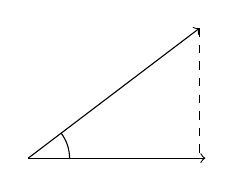
\begin{tikzpicture}[scale=0.75]
\draw[->] (0,0) -- (3,0);
\draw[->] (0,0) -- (2.9,2.2);
\draw[dashed] (2.9,2.2) -- (2.9,0);
\draw (0.7,0) arc (0:37:0.7);
\end{tikzpicture}}\ntag{D}{39}{keph103}{13}{}{Class XI Part 1 \textperiodcentered{} Ch 3}}
{\opt{3:1}{1:2}{4:1}{1:3}}
\numoptstrue
\QQ{\qsrc{2025}{3}In the projectile motion of a particle on a level ground, which of the following remains constant with reference to time and position?\ntag{D}{38}{keph103}{12}{}{Class XI Part 1 \textperiodcentered{} Ch 3}}
{\opt{Vertical component of the velocity of the projectile}{Average velocity between any two points on the path}{Horizontal component of velocity}{Angle between the instantaneous velocity with the horizontal}}
\numoptsfalse
\QQ{\qsrc{2022}{23}Two objects are projected at an angle $\theta^\circ$ and $(90-\theta)^\circ$, to the horizontal with the same speed. The ratio of their maximum vertical heights is\ntag{D}{39}{keph103}{13}{}{Class XI Part 1 \textperiodcentered{} Ch 3}}
{\opt{$1:\tan\theta$}{$1:1$}{$\tan^2\theta:1$}{$\tan\theta:1$}}
\numoptsfalse
\QQ{\qsrc{2021}{3}The maximum range of a gun on horizontal plane is $16\unit{km}$. If $g = 10\unit{m\,s^{-2}}$, then muzzle velocity of a shell is\ntag{D}{40}{keph103}{14}{}{Class XI Part 1 \textperiodcentered{} Ch 3}}
{\opt{$160\unit{m\,s^{-1}}$}{$200\sqrt2\unit{m\,s^{-1}}$}{$400\unit{m\,s^{-1}}$}{$800\unit{m\,s^{-1}}$}}
\numoptsfalse
\QQ{\qsrc{2021}{4}The trajectory of a projectile is\ntag{D}{39}{keph103}{13}{}{Class XI Part 1 \textperiodcentered{} Ch 3}}
{\opt{semicircle}{an ellipse}{a parabola always}{a parabola in the absence of air resistance}}
\numoptsfalse
\QQ{\qsrc{2021}{5}For a projectile motion, the angle between the velocity and acceleration is minimum and acute at\ntag{A}{39}{keph103}{13}{}{Class XI Part 1 \textperiodcentered{} Ch 3}\nsrc{None found in NEET/AIPMT/AIEEE/JEE papers, 2005--2026 (NCERT concept application)}}
{\opt{only one point}{two points}{three points}{four points}}
\numoptsfalse
\QQ{\qsrc{2019}{13}The trajectory of a projectile projected from origin is given by the equation $y = x-\dfrac{2x^2}{5}$. The initial velocity of the projectile is\ntag{A}{39}{keph103}{13}{}{Class XI Part 1 \textperiodcentered{} Ch 3}\nsrc{None found in NEET/AIPMT/AIEEE/JEE papers, 2005--2026 (NCERT concept application)}}
{\opt{$\dfrac25\unit{m\,s^{-1}}$}{$5\unit{m\,s^{-1}}$}{$25\unit{m\,s^{-1}}$}{$\dfrac52\unit{m\,s^{-1}}$}}
\numoptstrue
\QQ{\qsrc{2016}{2}Three projectiles A, B and C are projected at an angle of $30^\circ$, $45^\circ$, $60^\circ$ respectively. If $R_A$, $R_B$ and $R_C$ are ranges of A, B and C respectively, then (velocity of projection is same for A, B \& C)\ntag{D}{40}{keph103}{14}{}{Class XI Part 1 \textperiodcentered{} Ch 3}}
{\opt{$R_A = R_B = R_C$}{$R_A = R_C > R_B$}{$R_A<R_B<R_C$}{$R_A = R_C < R_B$}}
\topichead{Circular motion}{3}
\numoptstrue
\QQ{\qsrc{2025}{4}A particle is in uniform circular motion. The equation of its trajectory is given by $(x-2)^2+y^2 = 25$, where $x$ and $y$ are in meter. The speed of the particle is $2\unit{m\,s^{-1}}$. When the particle attains the lowest `$y$' co-ordinate, the acceleration of the particle is (in $\mathrm{m\,s^{-2}}$)\ntag{D}{41}{keph103}{15}{}{Class XI Part 1 \textperiodcentered{} Ch 3}}
{\opt{$0.4\,\hat i$}{$0.4\,\hat j$}{$0.8\,\hat i$}{$0.8\,\hat j$}}
\numoptsfalse
\QQ{\qsrc{2023}{14}A particle is in uniform circular motion. Related to one complete revolution of the particle, which among the statements is incorrect?\ntag{A}{40}{keph103}{14}{}{Class XI Part 1 \textperiodcentered{} Ch 3}\nsrc{None found in NEET/AIPMT/AIEEE/JEE papers, 2005--2026 (NCERT concept application)}}
{\opt{Displacement of the particle is zero.}{Average speed of the particle is zero.}{Average velocity of the particle is zero.}{Average acceleration of the particle is zero.}}
\numoptsfalse
\QQ{\qsrc{2017}{3}The angle between velocity and acceleration of a particle describing uniform circular motion is\ntag{D}{40}{keph103}{14}{}{Class XI Part 1 \textperiodcentered{} Ch 3}}
{\opt{$45^\circ$}{$60^\circ$}{$90^\circ$}{$180^\circ$}}
\end{multicols}
\par\needspace{12\baselineskip}\vspace{12pt}
\begin{center}{\pgfornament[width=3.2cm,color=gilt]{87}}\par
{\large\color{navy}\scshape Motion in a Plane \textperiodcentered{} Answer Key}\end{center}
{\small\setlength{\tabcolsep}{1pt}\renewcommand{\arraystretch}{1.5}
\begin{tabularx}{\linewidth}{@{}*{8}{>{\centering\arraybackslash}X}@{}}\toprule
\textbf{1}\,(A) & \textbf{2}\,(D) & \textbf{3}\,(B) & \textbf{4}\,(1) & \textbf{5}\,(D) & \textbf{6}\,(C) & \textbf{7}\,(D) & \textbf{8}\,(2)\\
\textbf{9}\,(3) & \textbf{10}\,(C) & \textbf{11}\,(C) & \textbf{12}\,(D) & \textbf{13}\,(A) & \textbf{14}\,(B) & \textbf{15}\,(4) & \textbf{16}\,(4)\\
\textbf{17}\,(B) & \textbf{18}\,(C) &  &  &  &  &  & \\\bottomrule\end{tabularx}}\par\smallskip
{\footnotesize Answers solved by the editor. Option labels are those of the original paper: (1)--(4) for 2016, 2025 and 2026, (A)--(D) for 2017--2024.
}\par
\par\needspace{18\baselineskip}\vspace{14pt}
\begin{center}{\pgfornament[width=3.2cm,color=gilt]{87}}\par
{\large\color{navy}\scshape Chapter Summary \textperiodcentered{} Motion in a Plane}\end{center}
{\small\setlength{\tabcolsep}{3.5pt}
\begin{tabular*}{\linewidth}{@{\extracolsep{\fill}}l*{11}{c}c@{}}\toprule
Year & 2016 & 2017 & 2018 & 2019 & 2020 & 2021 & 2022 & 2023 & 2024 & 2025 & 2026 & Total\\\midrule
Questions & 2 & 2 & 0 & 1 & 2 & 4 & 1 & 1 & 2 & 2 & 1 & \textbf{18}\\\bottomrule\end{tabular*}}\par\medskip
{\small\textbf{\color{crimson}Topic-wise} (in textbook order)\par\smallskip
\begin{tabularx}{\linewidth}{@{}>{\raggedright\arraybackslash}Xrrrl@{}}\toprule
Topic & Qs & Direct & Years & 2016 $\rightarrow$ 2026\\\midrule
Kinematics in one dimension & \textbf{1} & 0 & 1 & {\scriptsize {\color{gray!45}16} {\color{gray!45}17} {\color{gray!45}18} {\color{gray!45}19} {\color{gray!45}20} {\color{gray!45}21} {\color{gray!45}22} {\color{gray!45}23} \textbf{24} {\color{gray!45}25} {\color{gray!45}26}}\\
Vectors & \textbf{3} & 1 & 3 & {\scriptsize \textbf{16} \textbf{17} {\color{gray!45}18} {\color{gray!45}19} {\color{gray!45}20} {\color{gray!45}21} {\color{gray!45}22} {\color{gray!45}23} \textbf{24} {\color{gray!45}25} {\color{gray!45}26}}\\
Motion in a plane (vectors, relative velocity) & \textbf{3} & 2 & 2 & {\scriptsize {\color{gray!45}16} {\color{gray!45}17} {\color{gray!45}18} {\color{gray!45}19} \textbf{20} \textbf{21} {\color{gray!45}22} {\color{gray!45}23} {\color{gray!45}24} {\color{gray!45}25} {\color{gray!45}26}}\\
Projectile motion & \textbf{8} & 6 & 6 & {\scriptsize \textbf{16} {\color{gray!45}17} {\color{gray!45}18} \textbf{19} {\color{gray!45}20} \textbf{21} \textbf{22} {\color{gray!45}23} {\color{gray!45}24} \textbf{25} \textbf{26}}\\
Circular motion & \textbf{3} & 2 & 3 & {\scriptsize {\color{gray!45}16} \textbf{17} {\color{gray!45}18} {\color{gray!45}19} {\color{gray!45}20} {\color{gray!45}21} {\color{gray!45}22} \textbf{23} {\color{gray!45}24} \textbf{25} {\color{gray!45}26}}\\
\bottomrule\end{tabularx}}\par\medskip
\begin{minipage}[t]{0.34\linewidth}{\small\textbf{\color{crimson}Direct vs Applied}\par\smallskip
\begin{tabular}{@{}lrr@{}}\toprule
Direct from NCERT & \textbf{11} & 61\%\\
\quad text, table, figure & 9 &\\
\quad solved Example & 1 &\\
\quad Exercise & 1 &\\
Applied & \textbf{7} & 39\%\\\midrule
Easy / Mod. / Hard & \multicolumn{2}{r}{15 / 3 / 0}\\\bottomrule
\end{tabular}}\end{minipage}\hfill
\begin{minipage}[t]{0.63\linewidth}{\small\textbf{\color{crimson}What to focus on}\par\smallskip
\begin{itemize}[leftmargin=1.1em,itemsep=1pt,topsep=0pt]
\item 18 questions in 11 papers, about 1.6 per paper; rank 12 of 28 chapters by number of questions.
\item Most asked topic: \textbf{Projectile motion} (8 questions, in 6 of the 11 years).
\item 2 questions are NCERT solved Examples or Exercises: Example 3.1 (Q 7), Exercise 3.18 (Q 5). Work these by hand.
\item NCERT pages that gave three or more questions: page 39 (5 questions), page 40 (4 questions). Read these pages line by line.
\item Difficulty: 15 easy, 3 moderate, 0 hard.
\item 7 applied questions; 1 closely resemble a NEET/JEE/AIEEE question (marked in their tags).
\end{itemize}}\end{minipage}\par
\chapterpaper{Class XI \textperiodcentered{} Chapter 4}{Laws of Motion}{16 questions \textperiodcentered{} 5 topics \textperiodcentered{} KCET 2016--2026}{ckeph104}{XI.4 Laws of Motion}
\begin{multicols}{2}
\topichead{Laws of motion (lift, apparent weight)}{5}
\numoptstrue
\QQ{\qsrc{2026}{5}A man weighs $80\unit{kg}$. He stands on a weighing scale in a lift which is moving upwards with a uniform acceleration of $6\unit{m/s^2}$. What would be his weight in kg? ($g = 10\unit{m/s^2}$)\ntag{D}{69}{keph104}{21}{ \textperiodcentered{} Exercise 4.13}{Class XI Part 1 \textperiodcentered{} Ch 4}}
{\opt{Zero}{$48\unit{kg}$}{$120\unit{kg}$}{$128\unit{kg}$}}
\numoptsfalse
\QQ{\qsrc{2022}{20}Two masses of $5\unit{kg}$ and $3\unit{kg}$ are suspended with the help of massless inextensible strings as shown in fig. When whole system is going upwards with acceleration $2\unit{m/s^2}$, the value of $T_1$ is (use $g = 9.8\unit{m/s^2}$)
\fig{\begin{tikzpicture}[scale=0.75]
\fill[pattern=north east lines] (-1,2.6) rectangle (1,2.75); \draw (-1,2.6) -- (1,2.6);
\draw (0,2.6) -- (0,1.7); \draw[->] (0,2.0) -- (0,2.3) node[right,lbl]{$T_1$};
\draw[pattern=north east lines] (-0.3,1.1) rectangle (0.3,1.7); \node[lbl,right] at (0.35,1.4) {5 kg};
\draw (0,1.1) -- (0,0.5); \draw[->] (0,0.7) -- (0,1.0) node[right,lbl]{$T_2$};
\draw[pattern=north east lines] (-0.3,0) rectangle (0.3,0.5); \node[lbl,right] at (0.35,0.25) {3 kg};
\end{tikzpicture}}\ntag{A}{62}{keph104}{14}{}{Class XI Part 1 \textperiodcentered{} Ch 4}\nsrc{None found in NEET/AIPMT/AIEEE/JEE papers, 2005--2026 (NCERT concept application)}}
{\opt{$23.6\unit{N}$}{$94.4\unit{N}$}{$59\unit{N}$}{$35.4\unit{N}$}}
\numoptsfalse
\QQ{\qsrc{2019}{14}An object with mass $5\unit{kg}$ is acted upon by a force, $\vec F = (-3\hat i+4\hat j)\unit{N}$. If its initial velocity at $t = 0$ is $\vec v = (6\hat i-12\hat j)\unit{m\,s^{-1}}$, the time at which it will just have a velocity along $y$-axis is\ntag{A}{53}{keph104}{5}{}{Class XI Part 1 \textperiodcentered{} Ch 4}\nsrc{None found in NEET/AIPMT/AIEEE/JEE papers, 2005--2026 (NCERT concept application)}}
{\opt{$5\unit{s}$}{$10\unit{s}$}{$2\unit{s}$}{$15\unit{s}$}}
\numoptsfalse
\QQ{\qsrc{2018}{13}A man weighing $60\unit{kg}$ is in a lift moving down with an acceleration of $1.8\unit{m\,s^{-2}}$. The force exerted by the floor on him is\ntag{D}{69}{keph104}{21}{ \textperiodcentered{} Exercise 4.13}{Class XI Part 1 \textperiodcentered{} Ch 4}}
{\opt{$588\unit{N}$}{$480\unit{N}$}{Zero}{$696\unit{N}$}}
\numoptsfalse
\QQ{\qsrc{2017}{5}A body of mass $50\unit{kg}$ is suspended using a spring balance inside a lift at rest. If the lift starts falling freely, the reading of the spring balance is\ntag{D}{69}{keph104}{21}{ \textperiodcentered{} Exercise 4.13}{Class XI Part 1 \textperiodcentered{} Ch 4}}
{\opt{$= 50\unit{kg}$}{$> 50\unit{kg}$}{$< 50\unit{kg}$}{$= 0$}}
\topichead{Collisions and momentum conservation}{1}
\numoptstrue
\QQ{\qsrc{2016}{5}A $12\unit{kg}$ bomb at rest explodes into two pieces of $4\unit{kg}$ and $8\unit{kg}$. If the momentum of $4\unit{kg}$ piece is $20\unit{N\,s}$, the kinetic energy of the $8\unit{kg}$ piece is\ntag{A}{57}{keph104}{9}{}{Class XI Part 1 \textperiodcentered{} Ch 4}\nsrc{None found in NEET/AIPMT/AIEEE/JEE papers, 2005--2026 (NCERT concept application)}}
{\opt{$25\unit{J}$}{$20\unit{J}$}{$50\unit{J}$}{$40\unit{J}$}}
\topichead{Equilibrium of forces and tension}{1}
\numoptstrue
\QQ{\qsrc{2026}{6}A mass M is hung with a light inextensible string as shown in figure. Find the tension of the horizontal string.
\fig{\begin{tikzpicture}[scale=0.8]
\fill[pattern=north east lines] (0.9,2.5) rectangle (2.6,2.65);
\draw (0.9,2.5) -- (2.6,2.5);
\fill[pattern=north east lines] (-1.65,-0.8) rectangle (-1.5,1.2);
\draw (-1.5,-0.8) -- (-1.5,1.2);
\draw (0,0) -- (1.8,2.5) node[pos=0.55,sloped]{\tikz\draw[-{Stealth[length=4pt]}] (0,0)--(0.01,0);};
\draw (0,0) -- (-1.5,0) node[pos=0.5]{\tikz\draw[-{Stealth[length=4pt]}] (0.01,0)--(0,0);};
\draw (0,0) -- (0,-1.2) node[pos=0.5]{\tikz\draw[-{Stealth[length=4pt]}] (0,0.01)--(0,0);};
\draw (1.8,2.5) ++(-0.4,0) arc (180:234:0.4);
\node[lbl] at (1.15,2.2) {$45^\circ$};
\node[lbl,right] at (0,0) {O};
\draw[pattern=north east lines] (-0.25,-1.2) rectangle (0.25,-1.55);
\node[lbl,right] at (0.3,-1.38) {M};
\end{tikzpicture}}\ntag{D}{58}{keph104}{10}{ \textperiodcentered{} Example 4.6}{Class XI Part 1 \textperiodcentered{} Ch 4}}
{\opt{$\sqrt2\,Mg$}{$\sqrt3\,Mg$}{$Mg$}{$3\,Mg$}}
\topichead{Friction}{6}
\numoptstrue
\QQ{\qsrc{2025}{5}A wooden block of mass M lies on a rough floor. Another wooden block of the same mass is hanging from the point O through strings as shown in the figure. To achieve equilibrium, the co-efficient of static friction between the block on the floor with the floor itself is
\fig{\begin{tikzpicture}[scale=0.8]
\fill[pattern=north east lines] (-0.3,-0.12) rectangle (1.3,0);
\draw (-0.3,0) -- (1.3,0);
\draw (0,0) rectangle (0.8,0.6) node[midway,lbl]{M};
\draw (0.8,0.3) -- (2.6,0.3);
\fill (2.6,0.3) circle (1.2pt) node[above,lbl]{O};
\draw (2.6,0.3) -- (4.0,1.1);
\fill[pattern=north east lines] (4.0,0.5) rectangle (4.12,1.9); \draw (4.0,0.5)--(4.0,1.9);
\draw[dashed] (2.6,0.3) -- (3.5,0.3);
\draw (3.1,0.3) arc (0:29:0.5); \node[lbl] at (3.3,0.47) {$\theta$};
\draw (2.6,0.3) -- (2.6,-0.6);
\draw (2.3,-0.6) rectangle (2.9,-1.15) node[midway,lbl]{M};
\end{tikzpicture}}\ntag{A}{61}{keph104}{13}{}{Class XI Part 1 \textperiodcentered{} Ch 4}\nsrc{None found in NEET/AIPMT/AIEEE/JEE papers, 2005--2026 (NCERT concept application)}}
{\opt{$\mu = \cos\theta$}{$\mu = \cot\theta$}{$\mu = \sin\theta$}{$\mu = \tan\theta$}}
\numoptstrue
\QQ{\qsrc{2025}{6}A block of certain mass is placed on a rough floor. The coefficients of static and kinetic friction between the block and the floor are 0.4 and 0.25 respectively. A constant horizontal force $F = 20\unit{N}$ acts on it so that the velocity of the block varies with time according to the following graph. The mass of the block is nearly (Take $g\simeq10\unit{m\,s^{-2}}$)
\fig{\begin{tikzpicture}[xscale=0.55,yscale=0.09]
\foreach \x in {1,...,5} \draw[densely dotted] (\x,0) -- (\x,22);
\foreach \y in {5,10,15,20} {\draw[densely dotted] (0,\y) -- (5.5,\y); \node[lbl,left] at (0,\y) {\y};}
\draw[->] (0,0) -- (5.9,0) node[right,lbl]{$t$ (s)};
\draw[->] (0,0) -- (0,25) node[above,lbl]{$v$ (m/s)};
\foreach \x in {0,...,5} \node[lbl,below] at (\x,0) {\x};
\draw[line width=0.9pt] (0,0) -- (3,20);
\end{tikzpicture}}\ntag{A}{61}{keph104}{13}{}{Class XI Part 1 \textperiodcentered{} Ch 4}\nsrc{None found in NEET/AIPMT/AIEEE/JEE papers, 2005--2026 (NCERT concept application)}}
{\opt{$2.2\unit{kg}$}{$4.4\unit{kg}$}{$1.2\unit{kg}$}{$1.0\unit{kg}$}}
\numoptsfalse
\QQ{\qsrc{2024}{16}A block of certain mass is placed on a rough inclined plane. The angle between the plane and the horizontal is $30^\circ$. The coefficients of static and kinetic frictions between the block and the inclined plane are 0.6 and 0.5 respectively. Then the magnitude of the acceleration of the block is [Take $g = 10\unit{m\,s^{-2}}$]
\fig{\begin{tikzpicture}[scale=0.8]
\fill[pattern=north east lines] (0,-0.12) rectangle (3.2,0);
\draw (0,0) -- (3.2,0) -- (3.2,1.85) -- cycle;
\begin{scope}[shift={(1.3,0.75)},rotate=30]
\draw[pattern=north east lines] (0,0) rectangle (0.7,0.5);
\end{scope}
\draw (0.6,0) arc (0:30:0.6); \node[lbl] at (0.85,0.2) {$30^\circ$};
\end{tikzpicture}}\ntag{A}{61}{keph104}{13}{}{Class XI Part 1 \textperiodcentered{} Ch 4}\nsrc{None found in NEET/AIPMT/AIEEE/JEE papers, 2005--2026 (NCERT concept application)}}
{\opt{$2\unit{m\,s^{-2}}$}{zero}{$0.196\unit{m\,s^{-2}}$}{$0.67\unit{m\,s^{-2}}$}}
\numoptsfalse
\QQ{\qsrc{2023}{8}A body of mass $10\unit{kg}$ is kept on a horizontal surface. The coefficient of kinetic friction between the body and the surface is 0.5. A horizontal force of $60\unit{N}$ is applied on the body. The resulting acceleration of the body is about\ntag{A}{60}{keph104}{12}{}{Class XI Part 1 \textperiodcentered{} Ch 4}\nsrc{None found in NEET/AIPMT/AIEEE/JEE papers, 2005--2026 (NCERT concept application)}}
{\opt{$5\unit{m\,s^{-2}}$}{$6\unit{m\,s^{-2}}$}{zero}{$1\unit{m\,s^{-2}}$}}
\numoptsfalse
\QQ{\qsrc{2018}{8}A block rests on a rough inclined plane making an angle of $30^\circ$ with the horizontal. The coefficient of static friction between the block and the plane is 0.8. If the frictional force on the block is $10\unit{N}$, the mass of the block is ($g = 10\unit{m\,s^{-2}}$)\ntag{A}{61}{keph104}{13}{}{Class XI Part 1 \textperiodcentered{} Ch 4}\nsrc{None found in NEET/AIPMT/AIEEE/JEE papers, 2005--2026 (NCERT concept application)}}
{\opt{$1\unit{kg}$}{$2\unit{kg}$}{$3\unit{kg}$}{$4\unit{kg}$}}
\numoptstrue
\QQ{\qsrc{2016}{4}Maximum acceleration of the train in which a $50\unit{kg}$ box lying on its floor will remain stationary (Given: Co-efficient of static friction between the box and the train's floor is 0.3 and $g = 10\unit{m\,s^{-2}}$)\ntag{D}{61}{keph104}{13}{ \textperiodcentered{} Example 4.7}{Class XI Part 1 \textperiodcentered{} Ch 4}}
{\opt{$5.0\unit{m\,s^{-2}}$}{$3.0\unit{m\,s^{-2}}$}{$1.5\unit{m\,s^{-2}}$}{$15\unit{m\,s^{-2}}$}}
\topichead{Circular motion}{3}
\numoptsfalse
\QQ{\qsrc{2022}{24}A car is moving in a circular horizontal track of radius $10\unit{m}$ with a constant speed of $10\unit{m\,s^{-1}}$. A bob is suspended from the roof of the car by a light wire of length $1.0\unit{m}$. The angle made by the wire with the vertical is (in radian)\ntag{A}{63}{keph104}{15}{}{Class XI Part 1 \textperiodcentered{} Ch 4}\nsrc{None found in NEET/AIPMT/AIEEE/JEE papers, 2005--2026 (NCERT concept application)}}
{\opt{0}{$\dfrac\pi6$}{$\dfrac\pi3$}{$\dfrac\pi4$}}
\numoptsfalse
\QQ{\qsrc{2021}{7}A coin placed on a rotating turn table just slips if it is placed at a distance of $4\unit{cm}$ from the centre. If the angular velocity of the turn table is doubled it will just slip at a distance of:\ntag{A}{63}{keph104}{15}{}{Class XI Part 1 \textperiodcentered{} Ch 4}\nsrc{None found in NEET/AIPMT/AIEEE/JEE papers, 2005--2026 (NCERT concept application)}}
{\opt{$1\unit{cm}$}{$2\unit{cm}$}{$4\unit{cm}$}{$8\unit{cm}$}}
\numoptsfalse
\QQ{\qsrc{2020}{58}One end of a string of length `$l$' is connected to a particle of mass `$m$' and the other to a small peg on a smooth horizontal table. If the particle moves in a circle with speed `$v$', the net force on the particle (directed towards the centre) is: ($T$ is the tension in the string)\ntag{D}{69}{keph104}{21}{ \textperiodcentered{} Exercise 4.4}{Class XI Part 1 \textperiodcentered{} Ch 4}}
{\opt{$T$}{$T-\dfrac{mv^2}{l}$}{$T+\dfrac{mv^2}{l}$}{0}}
\end{multicols}
\par\needspace{12\baselineskip}\vspace{12pt}
\begin{center}{\pgfornament[width=3.2cm,color=gilt]{87}}\par
{\large\color{navy}\scshape Laws of Motion \textperiodcentered{} Answer Key}\end{center}
{\small\setlength{\tabcolsep}{1pt}\renewcommand{\arraystretch}{1.5}
\begin{tabularx}{\linewidth}{@{}*{8}{>{\centering\arraybackslash}X}@{}}\toprule
\textbf{1}\,(4) & \textbf{2}\,(B) & \textbf{3}\,(B) & \textbf{4}\,(B) & \textbf{5}\,(D) & \textbf{6}\,(1) & \textbf{7}\,(3) & \textbf{8}\,(2)\\
\textbf{9}\,(1) & \textbf{10}\,(B) & \textbf{11}\,(D) & \textbf{12}\,(B) & \textbf{13}\,(2) & \textbf{14}\,(D) & \textbf{15}\,(A) & \textbf{16}\,(A)\\\bottomrule\end{tabularx}}\par\smallskip
{\footnotesize Answers solved by the editor. Option labels are those of the original paper: (1)--(4) for 2016, 2025 and 2026, (A)--(D) for 2017--2024.
}\par
\par\needspace{18\baselineskip}\vspace{14pt}
\begin{center}{\pgfornament[width=3.2cm,color=gilt]{87}}\par
{\large\color{navy}\scshape Chapter Summary \textperiodcentered{} Laws of Motion}\end{center}
{\small\setlength{\tabcolsep}{3.5pt}
\begin{tabular*}{\linewidth}{@{\extracolsep{\fill}}l*{11}{c}c@{}}\toprule
Year & 2016 & 2017 & 2018 & 2019 & 2020 & 2021 & 2022 & 2023 & 2024 & 2025 & 2026 & Total\\\midrule
Questions & 2 & 1 & 2 & 1 & 1 & 1 & 2 & 1 & 1 & 2 & 2 & \textbf{16}\\\bottomrule\end{tabular*}}\par\medskip
{\small\textbf{\color{crimson}Topic-wise} (in textbook order)\par\smallskip
\begin{tabularx}{\linewidth}{@{}>{\raggedright\arraybackslash}Xrrrl@{}}\toprule
Topic & Qs & Direct & Years & 2016 $\rightarrow$ 2026\\\midrule
Laws of motion (lift, apparent weight) & \textbf{5} & 3 & 5 & {\scriptsize {\color{gray!45}16} \textbf{17} \textbf{18} \textbf{19} {\color{gray!45}20} {\color{gray!45}21} \textbf{22} {\color{gray!45}23} {\color{gray!45}24} {\color{gray!45}25} \textbf{26}}\\
Collisions and momentum conservation & \textbf{1} & 0 & 1 & {\scriptsize \textbf{16} {\color{gray!45}17} {\color{gray!45}18} {\color{gray!45}19} {\color{gray!45}20} {\color{gray!45}21} {\color{gray!45}22} {\color{gray!45}23} {\color{gray!45}24} {\color{gray!45}25} {\color{gray!45}26}}\\
Equilibrium of forces and tension & \textbf{1} & 1 & 1 & {\scriptsize {\color{gray!45}16} {\color{gray!45}17} {\color{gray!45}18} {\color{gray!45}19} {\color{gray!45}20} {\color{gray!45}21} {\color{gray!45}22} {\color{gray!45}23} {\color{gray!45}24} {\color{gray!45}25} \textbf{26}}\\
Friction & \textbf{6} & 1 & 5 & {\scriptsize \textbf{16} {\color{gray!45}17} \textbf{18} {\color{gray!45}19} {\color{gray!45}20} {\color{gray!45}21} {\color{gray!45}22} \textbf{23} \textbf{24} \textbf{25} {\color{gray!45}26}}\\
Circular motion & \textbf{3} & 1 & 3 & {\scriptsize {\color{gray!45}16} {\color{gray!45}17} {\color{gray!45}18} {\color{gray!45}19} \textbf{20} \textbf{21} \textbf{22} {\color{gray!45}23} {\color{gray!45}24} {\color{gray!45}25} {\color{gray!45}26}}\\
\bottomrule\end{tabularx}}\par\medskip
\begin{minipage}[t]{0.34\linewidth}{\small\textbf{\color{crimson}Direct vs Applied}\par\smallskip
\begin{tabular}{@{}lrr@{}}\toprule
Direct from NCERT & \textbf{6} & 38\%\\
\quad text, table, figure & 0 &\\
\quad solved Example & 2 &\\
\quad Exercise & 4 &\\
Applied & \textbf{10} & 62\%\\\midrule
Easy / Mod. / Hard & \multicolumn{2}{r}{7 / 9 / 0}\\\bottomrule
\end{tabular}}\end{minipage}\hfill
\begin{minipage}[t]{0.63\linewidth}{\small\textbf{\color{crimson}What to focus on}\par\smallskip
\begin{itemize}[leftmargin=1.1em,itemsep=1pt,topsep=0pt]
\item 16 questions in 11 papers, about 1.5 per paper; rank 13 of 28 chapters by number of questions.
\item Most asked topic: \textbf{Friction} (6 questions, in 5 of the 11 years).
\item 6 questions are NCERT solved Examples or Exercises: Example 4.6 (Q 7), Example 4.7 (Q 13), Exercise 4.13 (Q 1), Exercise 4.13 (Q 4), Exercise 4.13 (Q 5), Exercise 4.4 (Q 16). Work these by hand.
\item NCERT pages that gave three or more questions: page 61 (5 questions), page 69 (4 questions). Read these pages line by line.
\item Difficulty: 7 easy, 9 moderate, 0 hard.
\item 10 applied questions.
\end{itemize}}\end{minipage}\par
\chapterpaper{Class XI \textperiodcentered{} Chapter 5}{Work, Energy and Power}{14 questions \textperiodcentered{} 4 topics \textperiodcentered{} KCET 2016--2026}{ckeph105}{XI.5 Work, Energy and Power}
\begin{multicols}{2}
\topichead{Kinetic energy and momentum}{2}
\numoptstrue
\QQ{\qsrc{2026}{7}Two bodies with kinetic energies in the ratio of 3:1 are moving with equal linear momentum. The ratio of their masses is\ntag{A}{73}{keph105}{3}{}{Class XI Part 1 \textperiodcentered{} Ch 5}\nsrc{JEE Main 2021 (24 Feb, Shift 2) -- equal momentum, ratio of kinetic energies}}
{\opt{1:4}{1:3}{1:2}{1:1}}
\numoptsfalse
\QQ{\qsrc{2018}{9}Two particles of masses $m_1$ and $m_2$ have equal kinetic energies. The ratio of their momenta is\ntag{A}{74}{keph105}{4}{}{Class XI Part 1 \textperiodcentered{} Ch 5}\nsrc{None found in NEET/AIPMT/AIEEE/JEE papers, 2005--2026 (NCERT concept application)}}
{\opt{$m_1:m_2$}{$m_2:m_1$}{$\sqrt{m_1}:\sqrt{m_2}$}{$m_1^2:m_2^2$}}
\topichead{Work-energy theorem and power}{7}
\numoptstrue
\QQ{\qsrc{2026}{8}A horizontal force of $5\unit{N}$ is applied on a stationary body of mass $5\unit{kg}$, which is initially at rest on a frictionless table. The change in kinetic energy of the body in $10\unit{s}$ is\ntag{A}{73}{keph105}{3}{}{Class XI Part 1 \textperiodcentered{} Ch 5}\nsrc{None found in NEET/AIPMT/AIEEE/JEE papers, 2005--2026 (NCERT concept application)}}
{\opt{$25\unit{J}$}{Zero}{$125\unit{J}$}{$250\unit{J}$}}
\numoptstrue
\QQ{\qsrc{2025}{7}A body of mass $0.25\unit{kg}$ travels along a straight line from $x=0$ to $x=2\unit{m}$ with a speed $v = kx^{3/2}$ where $k = 2$ SI units. The work done by the net force during this displacement is\ntag{D}{73}{keph105}{3}{}{Class XI Part 1 \textperiodcentered{} Ch 5}}
{\opt{$4\unit{J}$}{$8\unit{J}$}{$16\unit{J}$}{$32\unit{J}$}}
\numoptsfalse
\QQ{\qsrc{2024}{17}A particle of mass $500\unit{g}$ is at rest. It is free to move along a straight line. The power delivered to the particle varies with time according to the following graph:
\fig{\begin{tikzpicture}[xscale=0.5,yscale=0.18]
\draw[->] (0,0) -- (6.6,0) node[right,lbl]{$t$ (s)};
\draw[->] (0,0) -- (0,13.5) node[above,lbl]{$P$ (watt)};
\foreach \x in {1,...,6} \node[lbl,below] at (\x,0) {\x};
\foreach \y in {2,4,...,12} {\draw (0.1,\y) -- (-0.1,\y) node[left,lbl]{\y};}
\draw (0,2) -- (6,9.2);
\draw[dashed] (0,8) -- (5,8) -- (5,0);
\fill (5,8) circle (4pt);
\end{tikzpicture}}
The momentum of the particle at $t = 5\unit{s}$ is\ntag{A}{83}{keph105}{13}{}{Class XI Part 1 \textperiodcentered{} Ch 5}\nsrc{None found in NEET/AIPMT/AIEEE/JEE papers, 2005--2026 (NCERT concept application)}}
{\opt{$2\sqrt5\unit{N\,s}$}{$5\sqrt2\unit{N\,s}$}{$5\unit{N\,s}$}{$5.5\unit{N\,s}$}}
\numoptsfalse
\QQ{\qsrc{2023}{9}A ball of mass $0.2\unit{kg}$ is thrown vertically down from a height of $10\unit{m}$. It collides with the floor and loses $50\%$ of its energy and then rises back to the same height. The value of its initial velocity is\ntag{A}{84}{keph105}{14}{}{Class XI Part 1 \textperiodcentered{} Ch 5}\nsrc{AIPMT 2015 (re-exam, Code A) -- ball thrown down, loses 50\% energy on impact and rebounds to the same height}}
{\opt{$14\unit{m\,s^{-1}}$}{$196\unit{m\,s^{-1}}$}{$20\unit{m\,s^{-1}}$}{zero}}
\numoptsfalse
\QQ{\qsrc{2022}{27}A smooth chain of length $2\unit{m}$ is kept on a table such that its length of $60\unit{cm}$ hangs freely from the edge of the table. The total mass of the chain is $4\unit{kg}$. The work done in pulling the entire chain on the table is, (Take $g = 10\unit{m/s^2}$)\ntag{A}{75}{keph105}{5}{}{Class XI Part 1 \textperiodcentered{} Ch 5}\nsrc{None found in NEET/AIPMT/AIEEE/JEE papers, 2005--2026 (NCERT concept application)}}
{\opt{$3.6\unit{J}$}{$12.9\unit{J}$}{$2.0\unit{J}$}{$6.3\unit{J}$}}
\numoptsfalse
\QQ{\qsrc{2020}{59}A body is initially at rest. It undergoes one-dimensional motion with constant acceleration. The power delivered to it at time `$t$' is proportional to\ntag{D}{90}{keph105}{20}{ \textperiodcentered{} Exercise 5.9}{Class XI Part 1 \textperiodcentered{} Ch 5}}
{\opt{$t^{1/2}$}{$t$}{$t^{3/2}$}{$t^2$}}
\numoptsfalse
\QQ{\qsrc{2017}{6}A motor pump lifts 6 tonnes of water from a well of depth $25\unit{m}$ to the first floor of height $35\unit{m}$ from the ground floor in 20 minutes. The power of the pump (in kW) is [$g = 10\unit{m\,s^{-2}}$]\ntag{D}{90}{keph105}{20}{ \textperiodcentered{} Exercise 5.15}{Class XI Part 1 \textperiodcentered{} Ch 5}}
{\opt{3}{6}{1.5}{12}}
\topichead{Collisions and momentum conservation}{4}
\numoptstrue
\QQ{\qsrc{2025}{8}During an elastic collision between two bodies, which of the following statements are correct?
\begin{stmts}
\item The initial kinetic energy is equal to the final kinetic energy of the system.
\item The linear momentum is conserved.
\item The kinetic energy during $\Delta t$ (the collision time) is not conserved.
\end{stmts}\ntag{D}{84}{keph105}{14}{}{Class XI Part 1 \textperiodcentered{} Ch 5}}
{\opt{I and II only}{II and III only}{I and III only}{I, II and III}}
\numoptsfalse
\QQ{\qsrc{2021}{9}A ball hits the floor and rebounds after an inelastic collision. In this case\ntag{A}{84}{keph105}{14}{}{Class XI Part 1 \textperiodcentered{} Ch 5}\nsrc{None found in NEET/AIPMT/AIEEE/JEE papers, 2005--2026 (NCERT concept application)}}
{\opt{the momentum of the ball is conserved}{the mechanical energy of the ball is conserved}{the total momentum of the ball and the earth is conserved}{the total mechanical energy of the ball and the earth is conserved}}
\numoptsfalse
\QQ{\qsrc{2021}{57}In a nuclear reactor heavy nuclei is not used as moderators because\ntag{D}{85}{keph105}{15}{ \textperiodcentered{} Example 5.11}{Class XI Part 1 \textperiodcentered{} Ch 5}}
{\opt{They will break up}{Elastic collision of neutrons with heavy nuclei will not slow them down.}{The net weight of the reactor would be unbearably high}{Substances with heavy nuclei do not occur in liquid or gaseous state at room temperature.}}
\numoptsfalse
\QQ{\qsrc{2019}{15}During inelastic collision between two objects, which of the following quantity always remains conserved?\ntag{D}{84}{keph105}{14}{}{Class XI Part 1 \textperiodcentered{} Ch 5}}
{\opt{Total kinetic energy}{Total mechanical energy}{Total linear momentum}{Speed of each body}}
\topichead{Mass defect, binding energy, fission and fusion}{1}
\numoptsfalse
\QQ{\qsrc{2017}{52}In a nuclear reactor the function of the Moderator is to decrease\ntag{D}{85}{keph105}{15}{ \textperiodcentered{} Example 5.11}{Class XI Part 1 \textperiodcentered{} Ch 5}}
{\opt{number of neutrons}{speed of neutrons}{escape of neutrons}{temperature of the reactor}}
\end{multicols}
\par\needspace{12\baselineskip}\vspace{12pt}
\begin{center}{\pgfornament[width=3.2cm,color=gilt]{87}}\par
{\large\color{navy}\scshape Work, Energy and Power \textperiodcentered{} Answer Key}\end{center}
{\small\setlength{\tabcolsep}{1pt}\renewcommand{\arraystretch}{1.5}
\begin{tabularx}{\linewidth}{@{}*{8}{>{\centering\arraybackslash}X}@{}}\toprule
\textbf{1}\,(2) & \textbf{2}\,(C) & \textbf{3}\,(4) & \textbf{4}\,(1) & \textbf{5}\,(C) & \textbf{6}\,(A) & \textbf{7}\,(A) & \textbf{8}\,(B)\\
\textbf{9}\,(A) & \textbf{10}\,(4) & \textbf{11}\,(C) & \textbf{12}\,(B) & \textbf{13}\,(C) & \textbf{14}\,(B) &  & \\\bottomrule\end{tabularx}}\par\smallskip
{\footnotesize Answers solved by the editor. Option labels are those of the original paper: (1)--(4) for 2016, 2025 and 2026, (A)--(D) for 2017--2024.
}\par
\par\needspace{18\baselineskip}\vspace{14pt}
\begin{center}{\pgfornament[width=3.2cm,color=gilt]{87}}\par
{\large\color{navy}\scshape Chapter Summary \textperiodcentered{} Work, Energy and Power}\end{center}
{\small\setlength{\tabcolsep}{3.5pt}
\begin{tabular*}{\linewidth}{@{\extracolsep{\fill}}l*{11}{c}c@{}}\toprule
Year & 2016 & 2017 & 2018 & 2019 & 2020 & 2021 & 2022 & 2023 & 2024 & 2025 & 2026 & Total\\\midrule
Questions & 0 & 2 & 1 & 1 & 1 & 2 & 1 & 1 & 1 & 2 & 2 & \textbf{14}\\\bottomrule\end{tabular*}}\par\medskip
{\small\textbf{\color{crimson}Topic-wise} (in textbook order)\par\smallskip
\begin{tabularx}{\linewidth}{@{}>{\raggedright\arraybackslash}Xrrrl@{}}\toprule
Topic & Qs & Direct & Years & 2016 $\rightarrow$ 2026\\\midrule
Kinetic energy and momentum & \textbf{2} & 0 & 2 & {\scriptsize {\color{gray!45}16} {\color{gray!45}17} \textbf{18} {\color{gray!45}19} {\color{gray!45}20} {\color{gray!45}21} {\color{gray!45}22} {\color{gray!45}23} {\color{gray!45}24} {\color{gray!45}25} \textbf{26}}\\
Work-energy theorem and power & \textbf{7} & 3 & 7 & {\scriptsize {\color{gray!45}16} \textbf{17} {\color{gray!45}18} {\color{gray!45}19} \textbf{20} {\color{gray!45}21} \textbf{22} \textbf{23} \textbf{24} \textbf{25} \textbf{26}}\\
Collisions and momentum conservation & \textbf{4} & 3 & 3 & {\scriptsize {\color{gray!45}16} {\color{gray!45}17} {\color{gray!45}18} \textbf{19} {\color{gray!45}20} \textbf{21} {\color{gray!45}22} {\color{gray!45}23} {\color{gray!45}24} \textbf{25} {\color{gray!45}26}}\\
Mass defect, binding energy, fission and fusion & \textbf{1} & 1 & 1 & {\scriptsize {\color{gray!45}16} \textbf{17} {\color{gray!45}18} {\color{gray!45}19} {\color{gray!45}20} {\color{gray!45}21} {\color{gray!45}22} {\color{gray!45}23} {\color{gray!45}24} {\color{gray!45}25} {\color{gray!45}26}}\\
\bottomrule\end{tabularx}}\par\medskip
\begin{minipage}[t]{0.34\linewidth}{\small\textbf{\color{crimson}Direct vs Applied}\par\smallskip
\begin{tabular}{@{}lrr@{}}\toprule
Direct from NCERT & \textbf{7} & 50\%\\
\quad text, table, figure & 3 &\\
\quad solved Example & 2 &\\
\quad Exercise & 2 &\\
Applied & \textbf{7} & 50\%\\\midrule
Easy / Mod. / Hard & \multicolumn{2}{r}{10 / 4 / 0}\\\bottomrule
\end{tabular}}\end{minipage}\hfill
\begin{minipage}[t]{0.63\linewidth}{\small\textbf{\color{crimson}What to focus on}\par\smallskip
\begin{itemize}[leftmargin=1.1em,itemsep=1pt,topsep=0pt]
\item 14 questions in 11 papers, about 1.3 per paper; rank 16 of 28 chapters by number of questions.
\item Most asked topic: \textbf{Work-energy theorem and power} (7 questions, in 7 of the 11 years).
\item 4 questions are NCERT solved Examples or Exercises: Example 5.11 (Q 12), Example 5.11 (Q 14), Exercise 5.9 (Q 8), Exercise 5.15 (Q 9). Work these by hand.
\item NCERT pages that gave three or more questions: page 84 (4 questions), page 73 (3 questions). Read these pages line by line.
\item Difficulty: 10 easy, 4 moderate, 0 hard.
\item 7 applied questions; 2 closely resemble a NEET/JEE/AIEEE question (marked in their tags).
\end{itemize}}\end{minipage}\par
\chapterpaper{Class XI \textperiodcentered{} Chapter 6}{System of Particles and Rotational Motion}{14 questions \textperiodcentered{} 3 topics \textperiodcentered{} KCET 2016--2026}{ckeph106}{XI.6 System of Particles and Rotational Motion}
\begin{multicols}{2}
\topichead{Centre of mass}{5}
\numoptstrue
\QQ{\qsrc{2025}{9}Three particles of mass $1\unit{kg}$, $2\unit{kg}$ and $3\unit{kg}$ are placed at the vertices A, B and C respectively of an equilateral triangle ABC of side $1\unit{m}$. The centre of mass of the system from vertex A (located at origin) is\ntag{D}{97}{keph106}{6}{ \textperiodcentered{} Example 6.1}{Class XI Part 1 \textperiodcentered{} Ch 6}}
{\opt{$(0,0)$}{$\left(\dfrac{7}{12},\dfrac{3\sqrt3}{12}\right)$}{$\left(\dfrac{9}{12},\dfrac{3\sqrt3}{12}\right)$}{$\left(\dfrac{7}{12},\dfrac{6+3\sqrt3}{12}\right)$}}
\numoptsfalse
\QQ{\qsrc{2022}{29}The centre of mass of an extended body on the surface of the earth and its centre of gravity\ntag{D}{113}{keph106}{22}{}{Class XI Part 1 \textperiodcentered{} Ch 6}}
{\opt{can never be at the same point.}{are always at the same point for any size of the body.}{centre of mass coincides with the centre of gravity of a body if the size of the body is negligible as compared to the size (or radius) of the earth.}{are always at the same point only for spherical bodies.}}
\numoptsfalse
\QQ{\qsrc{2019}{31}Two particles which are initially at rest move towards each other under the action of their mutual attraction. If their speeds are $v$ and $2v$ at any instant, then the speed of center of mass of the system is,\ntag{D}{99}{keph106}{8}{}{Class XI Part 1 \textperiodcentered{} Ch 6}}
{\opt{$2v$}{Zero}{$1.5v$}{$v$}}
\numoptsfalse
\QQ{\qsrc{2017}{7}Two balls are thrown simultaneously in air. The acceleration of the centre of mass of the two balls when in air,\ntag{D}{98}{keph106}{7}{}{Class XI Part 1 \textperiodcentered{} Ch 6}}
{\opt{depends on the masses of the two balls}{depends on the speeds of the two balls}{is equal to $g$ (Acceleration due to gravity)}{depends on the direction of motion of the two balls.}}
\numoptstrue
\QQ{\qsrc{2016}{6}Which of the points is likely position of the centre of mass of the system shown in the figure?
\fig{\begin{tikzpicture}[scale=0.85]
\fill[pattern=north east lines,pattern color=gray] (0,0) -- (2.4,0) -- (2.4,1.6) -- cycle;
\draw (0,0) rectangle (2.4,1.6); \draw (0,0) -- (2.4,1.6);
\node[lbl,rotate=34] at (0.35,1.3) {Air}; \node[lbl,rotate=34] at (1.9,0.55) {Sand};
\foreach \p/\n in {(0.65,1.25)/A,(0.9,1.05)/B,(1.2,0.82)/C,(1.42,0.6)/D} {\fill \p circle (1.3pt); \node[font=\tiny,above right] at \p {\n};}
\end{tikzpicture}}\ntag{A}{98}{keph106}{7}{}{Class XI Part 1 \textperiodcentered{} Ch 6}\nsrc{None found in NEET/AIPMT/AIEEE/JEE papers, 2005--2026 (NCERT concept application)}}
{\opt{A}{D}{B}{C}}
\topichead{Rotational dynamics (torque, moment of inertia)}{6}
\numoptstrue
\QQ{\qsrc{2025}{10}Two fly wheels are connected by a non-slipping belt as shown in the figure. $I_1 = 4\unit{kg\,m^2}$, $r_1 = 20\unit{cm}$, $I_2 = 20\unit{kg\,m^2}$ and $r_2 = 30\unit{cm}$. A torque of $10\unit{N\,m}$ is applied on the smaller wheel. Then match the entries of column I with appropriate entries of column II.\par\smallskip
{\small\begin{tabular}{@{}|l|p{0.44\linewidth}|l|c|@{}}\hline
I & Quantities & II & Value (SI)\\\hline
(a) & Angular acceleration of smaller wheel & (i) & $\frac53$\\[3pt]\hline
(b) & Torque on the larger wheel & (ii) & $\frac{100}{3}$\\[3pt]\hline
(c) & Angular acceleration of larger wheel & (iii) & $\frac52$\\[3pt]\hline
\end{tabular}}
\fig{\begin{tikzpicture}[scale=0.75]
\draw (0,0) circle (0.8); \draw (2.3,0) circle (1.2);
\draw ($(0,0)+(105:0.8)$) -- ($(2.3,0)+(97:1.2)$);
\draw ($(0,0)+(-105:0.8)$) -- ($(2.3,0)+(-97:1.2)$);
\draw[->] (0,0) -- (55:0.8) node[pos=0.6,right,lbl]{$r_1$};
\draw[->] (2.3,0) -- ($(2.3,0)+(120:1.2)$) node[pos=0.6,right,lbl]{$r_2$};
\fill (0,0) circle (1.5pt) (2.3,0) circle (1.5pt);
\end{tikzpicture}}\ntag{A}{119}{keph106}{28}{}{Class XI Part 1 \textperiodcentered{} Ch 6}\nsrc{None found in NEET/AIPMT/AIEEE/JEE papers, 2005--2026 (NCERT concept application)}}
{\opt{a--iii, b--ii, c--i}{a--ii, b--iii, c--i}{a--iii, b--i, c--ii}{a--ii, b--i, c--iii}}
\numoptsfalse
\QQ{\qsrc{2024}{21}A ceiling fan is rotating around a fixed axle as shown. The direction of angular velocity is along \rule{1.2cm}{0.4pt}.
\fig{\begin{tikzpicture}[scale=0.7]
\draw[densely dashed] (0,-1.6) -- (0,2.4);
\draw (-0.2,0.3) -- (-0.2,2.0) (0.2,0.3) -- (0.2,2.0); \draw (-0.2,2.0) -- (0.2,2.0);
\draw (-0.2,0.3) -- (-0.55,-0.15) -- (0.55,-0.15) -- (0.2,0.3);
\draw (-0.55,-0.15) -- (-0.55,-0.4) arc (180:360:0.55 and 0.15) -- (0.55,-0.15);
\draw[rotate around={-40:(-0.4,-0.3)}] (-0.4,-0.45) rectangle (-2.1,-0.15);
\draw[rotate around={40:(0.4,-0.3)}] (0.4,-0.45) rectangle (2.1,-0.15);
\draw[rotate around={-150:(-0.3,0.0)}] (-0.3,-0.12) rectangle (-1.9,0.18);
\draw[->] (0.28,-1.05) arc (0:-300:0.28 and 0.12);
\draw[densely dashed,->] (2.2,1.0) -- (2.2,2.0) node[right,lbl]{Z};
\draw[densely dashed,->] (2.2,1.0) -- (3.3,1.0) node[right,lbl]{Y};
\draw[densely dashed,->] (2.2,1.0) -- (1.6,0.4) node[below,lbl]{X};
\end{tikzpicture}}\ntag{D}{104}{keph106}{13}{}{Class XI Part 1 \textperiodcentered{} Ch 6}}
{\opt{$+\hat j$}{$-\hat j$}{$+\hat k$}{$-\hat k$}}
\numoptsfalse
\QQ{\qsrc{2024}{22}A body of mass $1\unit{kg}$ is suspended by a weightless string which passes over a frictionless pulley of mass $2\unit{kg}$ as shown in the figure. The mass is released from a height of $1.6\unit{m}$ from the ground. With what velocity does it strike the ground?
\fig{\begin{tikzpicture}[scale=0.75]
\draw (0,2.6) circle (0.55); \fill (0,2.6) circle (1.3pt); \node[lbl] at (0,2.85) {2 kg};
\draw (0,2.6) -- (1.4,2.6); \fill[pattern=north east lines] (1.4,1.9) rectangle (1.52,3.2); \draw (1.4,1.9) -- (1.4,3.2);
\draw (-0.55,2.6) -- (-0.55,0.9);
\draw[pattern=north east lines] (-0.75,0.55) rectangle (-0.35,0.9); \node[lbl,right] at (-0.3,0.72) {1 kg};
\draw[<->] (-0.55,0.55) -- (-0.55,0) node[midway,right,lbl]{1.6 m};
\fill[pattern=north east lines] (-1.4,-0.12) rectangle (1.6,0); \draw (-1.4,0) -- (1.6,0);
\end{tikzpicture}}\ntag{A}{120}{keph106}{29}{}{Class XI Part 1 \textperiodcentered{} Ch 6}\nsrc{None found in NEET/AIPMT/AIEEE/JEE papers, 2005--2026 (NCERT concept application)}}
{\opt{$16\unit{m\,s^{-1}}$}{$8\unit{m\,s^{-1}}$}{$4\sqrt2\unit{m\,s^{-1}}$}{$4\unit{m\,s^{-1}}$}}
\numoptsfalse
\QQ{\qsrc{2023}{10}The moment of inertia of a rigid body about an axis\ntag{D}{115}{keph106}{24}{}{Class XI Part 1 \textperiodcentered{} Ch 6}}
{\opt{does not depend on its shape.}{depends on the position of axis of rotation.}{does not depend on its size.}{does not depend on its mass.}}
\numoptsfalse
\QQ{\qsrc{2022}{28}The angular speed of a motor wheel is increased from $1200\unit{rpm}$ to $3120\unit{rpm}$ in 16 seconds. The angular acceleration of the motor wheel is\ntag{D}{117}{keph106}{26}{ \textperiodcentered{} Example 6.11}{Class XI Part 1 \textperiodcentered{} Ch 6}}
{\opt{$6\pi\unit{rad/s^2}$}{$2\pi\unit{rad/s^2}$}{$8\pi\unit{rad/s^2}$}{$4\pi\unit{rad/s^2}$}}
\numoptsfalse
\QQ{\qsrc{2020}{3}A wheel starting from rest gains an angular velocity of $10\unit{rad/s}$ after uniformly accelerated for $5\unit{sec}$. The total angle through which it has turned is\ntag{D}{117}{keph106}{26}{}{Class XI Part 1 \textperiodcentered{} Ch 6}}
{\opt{$25\unit{rad}$}{$100\unit{rad}$}{$25\pi\unit{rad}$}{$50\pi\unit{rad}$ about a vertical axis}}
\topichead{Angular momentum and its conservation}{3}
\numoptstrue
\QQ{\qsrc{2026}{9}The angular momentum of a moving body remains constant, if\ntag{D}{108}{keph106}{17}{}{Class XI Part 1 \textperiodcentered{} Ch 6}}
{\opt{net external force is applied}{net pressure is applied}{net external torque is applied}{net external torque is not applied}}
\numoptstrue
\QQ{\qsrc{2026}{10}If the earth were to suddenly contract to half of its present radius, what would be the duration of the day?\ntag{A}{122}{keph106}{31}{}{Class XI Part 1 \textperiodcentered{} Ch 6}\nsrc{JEE Main 2024 (6 Apr, Shift 1) -- earth's radius reduced, new length of day}}
{\opt{$6\unit{h}$}{$18\unit{h}$}{$24\unit{h}$}{$30\unit{h}$}}
\numoptsfalse
\QQ{\qsrc{2019}{32}A particle is moving uniformly along a straight line as shown in the figure. During the motion of the particle from A to B, the angular momentum of the particle about `O'
\fig{\begin{tikzpicture}[scale=0.8]
\draw[->] (-1.0,0) -- (2.2,0) node[right,lbl]{$x$}; \draw[->] (0,-0.8) -- (0,1.7) node[above,lbl]{$y$};
\node[lbl,below left] at (0,0) {O};
\draw (-0.9,-0.4) -- (1.0,1.5); \draw[->] (0.4,0.9) -- (0.6,1.1);
\fill (-0.3,0.2) circle (1.5pt) node[left,lbl]{A}; \fill (0.2,0.7) circle (1.5pt) node[below right,lbl]{P}; \node[lbl,left] at (0.75,1.3) {B};
\end{tikzpicture}}\ntag{A}{109}{keph106}{18}{}{Class XI Part 1 \textperiodcentered{} Ch 6}\nsrc{None found in NEET/AIPMT/AIEEE/JEE papers, 2005--2026 (NCERT concept application)}}
{\opt{increases}{decreases}{remains constant}{first increases then decreases}}
\end{multicols}
\par\needspace{12\baselineskip}\vspace{12pt}
\begin{center}{\pgfornament[width=3.2cm,color=gilt]{87}}\par
{\large\color{navy}\scshape System of Particles and Rotational Motion \textperiodcentered{} Answer Key}\end{center}
{\small\setlength{\tabcolsep}{1pt}\renewcommand{\arraystretch}{1.5}
\begin{tabularx}{\linewidth}{@{}*{8}{>{\centering\arraybackslash}X}@{}}\toprule
\textbf{1}\,(2) & \textbf{2}\,(C) & \textbf{3}\,(B) & \textbf{4}\,(C) & \textbf{5}\,(2) & \textbf{6}\,(1)$^{*}$ & \textbf{7}\,(D)$^{*}$ & \textbf{8}\,(D)\\
\textbf{9}\,(B) & \textbf{10}\,(D) & \textbf{11}\,(A) & \textbf{12}\,(4) & \textbf{13}\,(1) & \textbf{14}\,(C) &  & \\\bottomrule\end{tabularx}}\par\smallskip
{\footnotesize Answers solved by the editor. Option labels are those of the original paper: (1)--(4) for 2016, 2025 and 2026, (A)--(D) for 2017--2024. $^{*}$: see note.
\par\smallskip\textbf{6.} (KCET 2025 Q10) Intended answer; the given data treat each wheel separately.
\par\smallskip\textbf{7.} (KCET 2024 Q21) Viewed from above the fan turns clockwise, so the angular velocity points down.
}\par
\par\needspace{18\baselineskip}\vspace{14pt}
\begin{center}{\pgfornament[width=3.2cm,color=gilt]{87}}\par
{\large\color{navy}\scshape Chapter Summary \textperiodcentered{} System of Particles and Rotational Motion}\end{center}
{\small\setlength{\tabcolsep}{3.5pt}
\begin{tabular*}{\linewidth}{@{\extracolsep{\fill}}l*{11}{c}c@{}}\toprule
Year & 2016 & 2017 & 2018 & 2019 & 2020 & 2021 & 2022 & 2023 & 2024 & 2025 & 2026 & Total\\\midrule
Questions & 1 & 1 & 0 & 2 & 1 & 0 & 2 & 1 & 2 & 2 & 2 & \textbf{14}\\\bottomrule\end{tabular*}}\par\medskip
{\small\textbf{\color{crimson}Topic-wise} (in textbook order)\par\smallskip
\begin{tabularx}{\linewidth}{@{}>{\raggedright\arraybackslash}Xrrrl@{}}\toprule
Topic & Qs & Direct & Years & 2016 $\rightarrow$ 2026\\\midrule
Centre of mass & \textbf{5} & 4 & 5 & {\scriptsize \textbf{16} \textbf{17} {\color{gray!45}18} \textbf{19} {\color{gray!45}20} {\color{gray!45}21} \textbf{22} {\color{gray!45}23} {\color{gray!45}24} \textbf{25} {\color{gray!45}26}}\\
Rotational dynamics (torque, moment of inertia) & \textbf{6} & 4 & 5 & {\scriptsize {\color{gray!45}16} {\color{gray!45}17} {\color{gray!45}18} {\color{gray!45}19} \textbf{20} {\color{gray!45}21} \textbf{22} \textbf{23} \textbf{24} \textbf{25} {\color{gray!45}26}}\\
Angular momentum and its conservation & \textbf{3} & 1 & 2 & {\scriptsize {\color{gray!45}16} {\color{gray!45}17} {\color{gray!45}18} \textbf{19} {\color{gray!45}20} {\color{gray!45}21} {\color{gray!45}22} {\color{gray!45}23} {\color{gray!45}24} {\color{gray!45}25} \textbf{26}}\\
\bottomrule\end{tabularx}}\par\medskip
\begin{minipage}[t]{0.34\linewidth}{\small\textbf{\color{crimson}Direct vs Applied}\par\smallskip
\begin{tabular}{@{}lrr@{}}\toprule
Direct from NCERT & \textbf{9} & 64\%\\
\quad text, table, figure & 7 &\\
\quad solved Example & 2 &\\
\quad Exercise & 0 &\\
Applied & \textbf{5} & 36\%\\\midrule
Easy / Mod. / Hard & \multicolumn{2}{r}{10 / 4 / 0}\\\bottomrule
\end{tabular}}\end{minipage}\hfill
\begin{minipage}[t]{0.63\linewidth}{\small\textbf{\color{crimson}What to focus on}\par\smallskip
\begin{itemize}[leftmargin=1.1em,itemsep=1pt,topsep=0pt]
\item 14 questions in 11 papers, about 1.3 per paper; rank 18 of 28 chapters by number of questions.
\item Most asked topic: \textbf{Rotational dynamics (torque, moment of inertia)} (6 questions, in 5 of the 11 years).
\item 2 questions are NCERT solved Examples or Exercises: Example 6.1 (Q 1), Example 6.11 (Q 10). Work these by hand.
\item Difficulty: 10 easy, 4 moderate, 0 hard.
\item 5 applied questions; 1 closely resemble a NEET/JEE/AIEEE question (marked in their tags).
\end{itemize}}\end{minipage}\par
\chapterpaper{Class XI \textperiodcentered{} Chapter 7}{Gravitation}{14 questions \textperiodcentered{} 4 topics \textperiodcentered{} KCET 2016--2026}{ckeph107}{XI.7 Gravitation}
\begin{multicols}{2}
\topichead{Kepler's laws and planetary motion}{2}
\numoptstrue
\QQ{\qsrc{2025}{11}If $r_p, v_p, L_p$ and $r_a, v_a, L_a$ are radii, velocities and angular momenta of a planet at perihelion and aphelion of its elliptical orbit around the Sun respectively, then\ntag{D}{129}{keph107}{3}{ \textperiodcentered{} Example 7.1}{Class XI Part 1 \textperiodcentered{} Ch 7}}
{\opt{$r_p<r_a,\ v_p<v_a,\ L_a<L_p$}{$r_p>r_a,\ v_p>v_a,\ L_a>L_p$}{$r_p<r_a,\ v_p>v_a,\ L_a=L_p$}{$r_p>r_a,\ v_p<v_a,\ L_a=L_p$}}
\numoptsfalse
\QQ{\qsrc{2023}{17}When a planet revolves around the Sun, in general, for the planet\ntag{D}{128}{keph107}{2}{}{Class XI Part 1 \textperiodcentered{} Ch 7}}
{\opt{linear momentum and aerial velocity are constant.}{kinetic and potential energy of the planet are constant.}{angular momentum about the Sun and aerial velocity of the planet are constant.}{linear momentum and linear velocity are constant.}}
\topichead{Gravitation (force, field, energy)}{3}
\numoptstrue
\QQ{\qsrc{2026}{12}Suppose the acceleration due to gravity at the earth's surface is $g\unit{m/s^2}$ and at the surface of moon it is $g'\unit{m/s^2}$. An M kg passenger goes from the earth to the moon in a spaceship moving with a constant velocity (Neglect all other objects in the sky). Which curve best represents the weight (net gravitational force) as a function of time?
\fig{\begin{tikzpicture}[scale=0.9]
\draw[->] (0,0) -- (3.3,0) node[right,lbl]{$t$};
\draw[->] (0,0) -- (0,2.4);
\node[lbl,below left] at (0,0) {O};
\node[lbl,left] at (0,2) {$Mg$};
\node[lbl,left] at (0,1.2) {$Mg'$};
\draw[dashed] (0,1.2) -- (2.6,1.2) -- (2.6,0) node[below,lbl]{$t_0$};
\draw (0,2) -- (2.6,1.2) node[pos=0.35,above,lbl]{A};
\draw (0,2) .. controls (0.6,1.3) and (1.4,1.2) .. (2.6,1.2);
\node[lbl] at (1.0,1.5) {B};
\draw plot[smooth,tension=0.7] coordinates {(0,2)(0.45,0.85)(1.2,0.32)(1.95,0.55)(2.6,1.2)};
\node[lbl] at (1.55,0.62) {C};
\draw plot[smooth,tension=0.7] coordinates {(0,2)(0.35,0.7)(1.2,0.0)(2.0,0.4)(2.6,1.2)};
\node[lbl] at (0.95,-0.18) {D};
\end{tikzpicture}}\ntag{A}{132}{keph107}{6}{}{Class XI Part 1 \textperiodcentered{} Ch 7}\nsrc{None found in NEET/AIPMT/AIEEE/JEE papers, 2005--2026 (NCERT concept application)}}
{\opt{A}{B}{C}{D}}
\numoptsfalse
\QQ{\qsrc{2021}{11}Two bodies of masses $8\unit{kg}$ are placed at the vertices A and B of an equilateral triangle ABC. A third body of mass $2\unit{kg}$ is placed at the centroid G of the triangle. If $AG = BG = CG = 1\unit{m}$, where should a fourth body of mass $4\unit{kg}$ be placed so that the resultant force on the $2\unit{kg}$ body is zero?\ntag{A}{131}{keph107}{5}{}{Class XI Part 1 \textperiodcentered{} Ch 7}\nsrc{None found in NEET/AIPMT/AIEEE/JEE papers, 2005--2026 (NCERT concept application)}}
{\opt{at C}{at a point P on the line CG such that $PG = \dfrac{1}{\sqrt2}\unit{m}$}{at a point P on the line CG such that $PG = 0.5\unit{m}$}{at a point P on the line CG such that $PG = 2\unit{m}$}}
\numoptsfalse
\QQ{\qsrc{2018}{5}A mass `$m$' on the surface of the Earth is shifted to a target equal to the radius of the Earth. If `$R$' is the radius and `$M$' is the mass of the Earth, then work done in this process is\ntag{A}{134}{keph107}{8}{ \textperiodcentered{} Exemplar 8.32}{Class XI Part 1 \textperiodcentered{} Ch 7}\nsrc{None found in NEET/AIPMT/AIEEE/JEE papers, 2005--2026 (NCERT concept application)}}
{\opt{$\dfrac{mgR}{2}$}{$mgR$}{$2mgR$}{$\dfrac{mgR}{4}$}}
\topichead{Acceleration due to gravity (g, variation)}{6}
\numoptstrue
\QQ{\qsrc{2026}{11}Imagine a new planet having the same density as that of the earth, but it is two times bigger than the earth in size. If the acceleration due to gravity on the surface of the earth is $g$ and that on the surface of the new planet is $g'$, then\ntag{A}{132}{keph107}{6}{}{Class XI Part 1 \textperiodcentered{} Ch 7}\nsrc{NEET 2016 (Phase I) -- planet with radius and density twice that of earth}}
{\opt{$g' = \dfrac{g}{4}$}{$g' = 8g$}{$g' = 2g$}{$g' = 4g$}}
\numoptsfalse
\QQ{\qsrc{2024}{23}What is the value of acceleration due to gravity at a height equal to half the radius of the Earth, from its surface?\ntag{D}{133}{keph107}{7}{}{Class XI Part 1 \textperiodcentered{} Ch 7}}
{\opt{$4.4\unit{m\,s^{-2}}$}{$6.5\unit{m\,s^{-2}}$}{zero}{$9.8\unit{m\,s^{-2}}$}}
\numoptsfalse
\QQ{\qsrc{2020}{1}The value of acceleration due to gravity at a height of $10\unit{km}$ from the surface of earth is $x$. At what depth inside the earth is the value of the acceleration due to gravity has the same value $x$?\ntag{D}{134}{keph107}{8}{}{Class XI Part 1 \textperiodcentered{} Ch 7}}
{\opt{$5\unit{km}$}{$20\unit{km}$}{$10\unit{km}$}{$15\unit{km}$}}
\numoptsfalse
\QQ{\qsrc{2018}{2}Which of the following graphs correctly represents the variation of `$g$' on the Earth?\ntag{D}{134}{keph107}{8}{}{Class XI Part 1 \textperiodcentered{} Ch 7}}
{\optfig{\gaxes{$r$}{$g$}{\draw (0,0) -- (0.8,1.2) -- (1.7,0); \draw[densely dashed] (0.8,1.2) -- (0.8,0) node[below,font=\tiny]{R};}}
{\gaxes{$r$}{$g$}{\draw (0,0) -- (0.8,1.2) .. controls (1.0,0.6) and (1.3,0.45) .. (1.8,0.4); \draw[densely dashed] (0.8,1.2) -- (0.8,0) node[below,font=\tiny]{R};}}
{\gaxes{$r$}{$g$}{\draw (0,0) -- (0.8,1.2) -- (1.8,1.2); \draw[densely dashed] (0.8,1.2) -- (0.8,0) node[below,font=\tiny]{R};}}
{\gaxes{$r$}{$g$}{\draw (0,1.2) -- (0.8,1.2) -- (1.7,0); \draw[densely dashed] (0.8,1.2) -- (0.8,0) node[below,font=\tiny]{R};}}}
\numoptsfalse
\QQ{\qsrc{2017}{8}The value of acceleration due to gravity at a depth of $1600\unit{km}$ is equal to [Radius of earth $= 6400\unit{km}$]\ntag{D}{134}{keph107}{8}{}{Class XI Part 1 \textperiodcentered{} Ch 7}}
{\opt{$9.8\unit{m\,s^{-2}}$}{$4.9\unit{m\,s^{-2}}$}{$19.6\unit{m\,s^{-2}}$}{$7.35\unit{m\,s^{-2}}$}}
\numoptstrue
\QQ{\qsrc{2016}{8}Variation of acceleration due to gravity ($g$) with distance $x$ from the centre of the earth is best represented by ($R\to$ Radius of the earth)\ntag{D}{134}{keph107}{8}{}{Class XI Part 1 \textperiodcentered{} Ch 7}}
{\optfig{\gaxes{$x$}{$g$}{\draw (0,1.5) -- (0.8,0.6) .. controls (1.1,1.1) and (1.4,1.25) .. (1.9,1.3); \draw[densely dotted] (0.8,0.6) -- (0.8,0) node[below,font=\tiny]{R};}}
{\gaxes{$x$}{$g$}{\draw (0,0) -- (1.6,1.7); \draw[densely dotted] (0.8,0.85) -- (0.8,0) node[below,font=\tiny]{R};}}
{\gaxes{$x$}{$g$}{\draw (0,1.6) -- (0.8,0.7) .. controls (1.1,0.35) and (1.4,0.25) .. (1.9,0.2); \draw[densely dotted] (0.8,0.7) -- (0.8,0) node[below,font=\tiny]{R};}}
{\gaxes{$x$}{$g$}{\draw (0,0) -- (0.8,1.4) .. controls (1.0,0.6) and (1.3,0.3) .. (1.9,0.2); \draw[densely dotted] (0.8,1.4) -- (0.8,0) node[below,font=\tiny]{R};}}}
\topichead{Satellites, orbital and escape speed}{3}
\numoptstrue
\QQ{\qsrc{2025}{12}The total energy of a satellite in a circular orbit at a distance $(R+h)$ from the center of the Earth varies as [$R$ is the radius of the Earth and $h$ is the height of the orbit from Earth's surface]\ntag{D}{138}{keph107}{12}{}{Class XI Part 1 \textperiodcentered{} Ch 7}}
{\opt{$\dfrac{1}{R+h}$}{$-\dfrac{1}{R+h}$}{$\dfrac{1}{(R+h)^2}$}{$-\dfrac{1}{(R+h)^2}$}}
\numoptsfalse
\QQ{\qsrc{2019}{33}A satellite is orbiting close to the earth and has a kinetic energy K. The minimum extra kinetic energy required by it to just overcome the gravitation pull of the earth is\ntag{A}{135}{keph107}{9}{}{Class XI Part 1 \textperiodcentered{} Ch 7}\nsrc{None found in NEET/AIPMT/AIEEE/JEE papers, 2005--2026 (NCERT concept application)}}
{\opt{K}{2K}{$\sqrt3$K}{$2\sqrt2$K}}
\numoptsfalse
\QQ{\qsrc{2018}{60}A space station is at a height equal to the radius of the Earth. If `$v_E$' is the escape velocity on the surface of the Earth, the same on the space station is \rule{1cm}{0.4pt} times $v_E$.\ntag{A}{135}{keph107}{9}{}{Class XI Part 1 \textperiodcentered{} Ch 7}\nsrc{None found in NEET/AIPMT/AIEEE/JEE papers, 2005--2026 (NCERT concept application)}}
{\opt{$\dfrac12$}{$\dfrac14$}{$\dfrac1{\sqrt2}$}{$\dfrac1{\sqrt3}$}}
\end{multicols}
\par\needspace{12\baselineskip}\vspace{12pt}
\begin{center}{\pgfornament[width=3.2cm,color=gilt]{87}}\par
{\large\color{navy}\scshape Gravitation \textperiodcentered{} Answer Key}\end{center}
{\small\setlength{\tabcolsep}{1pt}\renewcommand{\arraystretch}{1.5}
\begin{tabularx}{\linewidth}{@{}*{8}{>{\centering\arraybackslash}X}@{}}\toprule
\textbf{1}\,(3) & \textbf{2}\,(C) & \textbf{3}\,(4) & \textbf{4}\,(B) & \textbf{5}\,(A) & \textbf{6}\,(3) & \textbf{7}\,(A) & \textbf{8}\,(B)\\
\textbf{9}\,(B) & \textbf{10}\,(D) & \textbf{11}\,(4) & \textbf{12}\,(2) & \textbf{13}\,(A) & \textbf{14}\,(C) &  & \\\bottomrule\end{tabularx}}\par\smallskip
{\footnotesize Answers solved by the editor. Option labels are those of the original paper: (1)--(4) for 2016, 2025 and 2026, (A)--(D) for 2017--2024.
}\par
\par\needspace{18\baselineskip}\vspace{14pt}
\begin{center}{\pgfornament[width=3.2cm,color=gilt]{87}}\par
{\large\color{navy}\scshape Chapter Summary \textperiodcentered{} Gravitation}\end{center}
{\small\setlength{\tabcolsep}{3.5pt}
\begin{tabular*}{\linewidth}{@{\extracolsep{\fill}}l*{11}{c}c@{}}\toprule
Year & 2016 & 2017 & 2018 & 2019 & 2020 & 2021 & 2022 & 2023 & 2024 & 2025 & 2026 & Total\\\midrule
Questions & 1 & 1 & 3 & 1 & 1 & 1 & 0 & 1 & 1 & 2 & 2 & \textbf{14}\\\bottomrule\end{tabular*}}\par\medskip
{\small\textbf{\color{crimson}Topic-wise} (in textbook order)\par\smallskip
\begin{tabularx}{\linewidth}{@{}>{\raggedright\arraybackslash}Xrrrl@{}}\toprule
Topic & Qs & Direct & Years & 2016 $\rightarrow$ 2026\\\midrule
Kepler's laws and planetary motion & \textbf{2} & 2 & 2 & {\scriptsize {\color{gray!45}16} {\color{gray!45}17} {\color{gray!45}18} {\color{gray!45}19} {\color{gray!45}20} {\color{gray!45}21} {\color{gray!45}22} \textbf{23} {\color{gray!45}24} \textbf{25} {\color{gray!45}26}}\\
Gravitation (force, field, energy) & \textbf{3} & 0 & 3 & {\scriptsize {\color{gray!45}16} {\color{gray!45}17} \textbf{18} {\color{gray!45}19} {\color{gray!45}20} \textbf{21} {\color{gray!45}22} {\color{gray!45}23} {\color{gray!45}24} {\color{gray!45}25} \textbf{26}}\\
Acceleration due to gravity (g, variation) & \textbf{6} & 5 & 6 & {\scriptsize \textbf{16} \textbf{17} \textbf{18} {\color{gray!45}19} \textbf{20} {\color{gray!45}21} {\color{gray!45}22} {\color{gray!45}23} \textbf{24} {\color{gray!45}25} \textbf{26}}\\
Satellites, orbital and escape speed & \textbf{3} & 1 & 3 & {\scriptsize {\color{gray!45}16} {\color{gray!45}17} \textbf{18} \textbf{19} {\color{gray!45}20} {\color{gray!45}21} {\color{gray!45}22} {\color{gray!45}23} {\color{gray!45}24} \textbf{25} {\color{gray!45}26}}\\
\bottomrule\end{tabularx}}\par\medskip
\begin{minipage}[t]{0.34\linewidth}{\small\textbf{\color{crimson}Direct vs Applied}\par\smallskip
\begin{tabular}{@{}lrr@{}}\toprule
Direct from NCERT & \textbf{8} & 57\%\\
\quad text, table, figure & 7 &\\
\quad solved Example & 1 &\\
\quad Exercise & 0 &\\
Applied & \textbf{6} & 43\%\\\midrule
Easy / Mod. / Hard & \multicolumn{2}{r}{7 / 7 / 0}\\\bottomrule
\end{tabular}}\end{minipage}\hfill
\begin{minipage}[t]{0.63\linewidth}{\small\textbf{\color{crimson}What to focus on}\par\smallskip
\begin{itemize}[leftmargin=1.1em,itemsep=1pt,topsep=0pt]
\item 14 questions in 11 papers, about 1.3 per paper; rank 15 of 28 chapters by number of questions.
\item Most asked topic: \textbf{Acceleration due to gravity (g, variation)} (6 questions, in 6 of the 11 years).
\item 1 questions are NCERT solved Examples or Exercises: Example 7.1 (Q 1). Work these by hand.
\item NCERT pages that gave three or more questions: page 134 (5 questions). Read these pages line by line.
\item Difficulty: 7 easy, 7 moderate, 0 hard.
\item 6 applied questions; 1 closely resemble a NEET/JEE/AIEEE question (marked in their tags).
\end{itemize}}\end{minipage}\par
\chapterpaper{Class XI \textperiodcentered{} Chapter 8}{Mechanical Properties of Solids}{10 questions \textperiodcentered{} 1 topics \textperiodcentered{} KCET 2016--2026}{ckeph201}{XI.8 Mechanical Properties of Solids}
\begin{multicols}{2}
\topichead{Elasticity (Young's modulus)}{10}
\numoptstrue
\QQ{\qsrc{2026}{14}There are two wires of same material and same length while the diameter of second wire is two times the diameter of the first wire. Then the ratio of extensions produced in the wires by applying same load will be\ntag{D}{170}{keph201}{4}{}{Class XI Part 2 \textperiodcentered{} Ch 8}}
{\opt{1:1}{1:2}{2:1}{4:1}}
\numoptstrue
\QQ{\qsrc{2025}{13}Two wires A and B are made of same material. Their diameters are in the ratio of 1:2 and lengths are in the ratio of 1:3. If they are stretched by the same force, then increase in their lengths will be in the ratio of\ntag{D}{170}{keph201}{4}{}{Class XI Part 2 \textperiodcentered{} Ch 8}}
{\opt{4:3}{3:4}{2:3}{3:2}}
\numoptsfalse
\QQ{\qsrc{2024}{24}A thick metal wire of density $\rho$ and length `$L$' is hung from a rigid support. The increase in length of the wire due to its own weight is ($Y$ = Young's modulus of the material of the wire)\ntag{A}{171}{keph201}{5}{}{Class XI Part 2 \textperiodcentered{} Ch 8}\nsrc{JEE Main 2022 (26 Jul, Shift 2) -- elongation of a hanging rod due to its own weight}}
{\opt{$\dfrac{\rho gL}{Y}$}{$\dfrac12\dfrac{\rho gL^2}{Y}$}{$\dfrac{\rho gL^2}{Y}$}{$\dfrac{1}{4Y}\rho gL^2$}}
\numoptsfalse
\QQ{\qsrc{2023}{18}A stretched wire of a material whose Young's modulus $Y = 2\times10^{11}\unit{N\,m^{-2}}$ has Poisson's ratio 0.25. Its lateral strain $\varepsilon_l = 10^{-3}$. The elastic energy density of the wire is\ntag{A}{174}{keph201}{8}{}{Class XI Part 2 \textperiodcentered{} Ch 8}\nsrc{None found in NEET/AIPMT/AIEEE/JEE papers, 2005--2026 (NCERT concept application)}}
{\opt{$1\times10^5\unit{J\,m^{-3}}$}{$4\times10^5\unit{J\,m^{-3}}$}{$8\times10^5\unit{J\,m^{-3}}$}{$16\times10^5\unit{J\,m^{-3}}$}}
\numoptsfalse
\QQ{\qsrc{2022}{30}A metallic rod breaks when strain produced is 0.2\%. The Young's modulus of the material of the rod is $7\times10^9\unit{N/m^2}$. The area of cross section to support a load of $10^4\unit{N}$ is\ntag{A}{171}{keph201}{5}{}{Class XI Part 2 \textperiodcentered{} Ch 8}\nsrc{None found in NEET/AIPMT/AIEEE/JEE papers, 2005--2026 (NCERT concept application)}}
{\opt{$7.1\times10^{-4}\unit{m^2}$}{$7.1\times10^{-8}\unit{m^2}$}{$7.1\times10^{-2}\unit{m^2}$}{$7.1\times10^{-6}\unit{m^2}$}}
\numoptsfalse
\QQ{\qsrc{2020}{2}Young's modulus of a perfect rigid body is\ntag{A}{170}{keph201}{4}{}{Class XI Part 2 \textperiodcentered{} Ch 8}\nsrc{None found in NEET/AIPMT/AIEEE/JEE papers, 2005--2026 (NCERT concept application)}}
{\opt{zero}{unity}{infinity}{between zero and unity}}
\numoptsfalse
\QQ{\qsrc{2019}{34}A wire is stretched such that its volume remains constant. The Poission's ratio of the material of the wire is\ntag{A}{174}{keph201}{8}{}{Class XI Part 2 \textperiodcentered{} Ch 8}\nsrc{None found in NEET/AIPMT/AIEEE/JEE papers, 2005--2026 (NCERT concept application)}}
{\opt{0.50}{$-0.50$}{0.25}{$-0.25$}}
\numoptsfalse
\QQ{\qsrc{2018}{15}Two wires A and B are stretched by the same load. If the area of cross-section of wire `A' is double that of `B', then the stress on `B' is\ntag{D}{169}{keph201}{3}{}{Class XI Part 2 \textperiodcentered{} Ch 8}}
{\opt{Equal to that on A}{Twice that on A}{Half that on A}{Four times that on A}}
\numoptsfalse
\QQ{\qsrc{2017}{9}`Young's modulus' is defined as the ratio of\ntag{D}{170}{keph201}{4}{}{Class XI Part 2 \textperiodcentered{} Ch 8}}
{\opt{tensile stress and longitudinal strain}{hydraulic stress and hydraulic strain}{shearing stress and shearing strain}{bulk stress and longitudinal strain}}
\numoptstrue
\QQ{\qsrc{2016}{9}A spring is stretched by applying a load to its free end. The strain produced in the spring is\ntag{A}{170}{keph201}{4}{ \textperiodcentered{} Exemplar 9.4}{Class XI Part 2 \textperiodcentered{} Ch 8}\nsrc{None found in NEET/AIPMT/AIEEE/JEE papers, 2005--2026 (NCERT concept application)}}
{\opt{Volumetric}{Shear}{Longitudinal \& Shear}{Longitudinal}}
\end{multicols}
\par\needspace{12\baselineskip}\vspace{12pt}
\begin{center}{\pgfornament[width=3.2cm,color=gilt]{87}}\par
{\large\color{navy}\scshape Mechanical Properties of Solids \textperiodcentered{} Answer Key}\end{center}
{\small\setlength{\tabcolsep}{1pt}\renewcommand{\arraystretch}{1.5}
\begin{tabularx}{\linewidth}{@{}*{8}{>{\centering\arraybackslash}X}@{}}\toprule
\textbf{1}\,(4) & \textbf{2}\,(1) & \textbf{3}\,(B) & \textbf{4}\,(D) & \textbf{5}\,(A) & \textbf{6}\,(C) & \textbf{7}\,(A) & \textbf{8}\,(B)\\
\textbf{9}\,(A) & \textbf{10}\,(2) &  &  &  &  &  & \\\bottomrule\end{tabularx}}\par\smallskip
{\footnotesize Answers solved by the editor. Option labels are those of the original paper: (1)--(4) for 2016, 2025 and 2026, (A)--(D) for 2017--2024.
}\par
\par\needspace{18\baselineskip}\vspace{14pt}
\begin{center}{\pgfornament[width=3.2cm,color=gilt]{87}}\par
{\large\color{navy}\scshape Chapter Summary \textperiodcentered{} Mechanical Properties of Solids}\end{center}
{\small\setlength{\tabcolsep}{3.5pt}
\begin{tabular*}{\linewidth}{@{\extracolsep{\fill}}l*{11}{c}c@{}}\toprule
Year & 2016 & 2017 & 2018 & 2019 & 2020 & 2021 & 2022 & 2023 & 2024 & 2025 & 2026 & Total\\\midrule
Questions & 1 & 1 & 1 & 1 & 1 & 0 & 1 & 1 & 1 & 1 & 1 & \textbf{10}\\\bottomrule\end{tabular*}}\par\medskip
{\small\textbf{\color{crimson}Topic-wise} (in textbook order)\par\smallskip
\begin{tabularx}{\linewidth}{@{}>{\raggedright\arraybackslash}Xrrrl@{}}\toprule
Topic & Qs & Direct & Years & 2016 $\rightarrow$ 2026\\\midrule
Elasticity (Young's modulus) & \textbf{10} & 4 & 10 & {\scriptsize \textbf{16} \textbf{17} \textbf{18} \textbf{19} \textbf{20} {\color{gray!45}21} \textbf{22} \textbf{23} \textbf{24} \textbf{25} \textbf{26}}\\
\bottomrule\end{tabularx}}\par\medskip
\begin{minipage}[t]{0.34\linewidth}{\small\textbf{\color{crimson}Direct vs Applied}\par\smallskip
\begin{tabular}{@{}lrr@{}}\toprule
Direct from NCERT & \textbf{4} & 40\%\\
\quad text, table, figure & 4 &\\
\quad solved Example & 0 &\\
\quad Exercise & 0 &\\
Applied & \textbf{6} & 60\%\\\midrule
Easy / Mod. / Hard & \multicolumn{2}{r}{7 / 3 / 0}\\\bottomrule
\end{tabular}}\end{minipage}\hfill
\begin{minipage}[t]{0.63\linewidth}{\small\textbf{\color{crimson}What to focus on}\par\smallskip
\begin{itemize}[leftmargin=1.1em,itemsep=1pt,topsep=0pt]
\item 10 questions in 11 papers, about 0.9 per paper; rank 23 of 28 chapters by number of questions.
\item Most asked topic: \textbf{Elasticity (Young's modulus)} (10 questions, in 10 of the 11 years).
\item Asked in 8 or more of the 11 years: Elasticity (Young's modulus).
\item NCERT pages that gave three or more questions: page 170 (5 questions). Read these pages line by line.
\item Difficulty: 7 easy, 3 moderate, 0 hard.
\item 6 applied questions; 1 closely resemble a NEET/JEE/AIEEE question (marked in their tags).
\end{itemize}}\end{minipage}\par
\chapterpaper{Class XI \textperiodcentered{} Chapter 9}{Mechanical Properties of Fluids}{13 questions \textperiodcentered{} 3 topics \textperiodcentered{} KCET 2016--2026}{ckeph202}{XI.9 Mechanical Properties of Fluids}
\begin{multicols}{2}
\topichead{Bernoulli's principle and fluid flow}{9}
\numoptstrue
\QQ{\qsrc{2026}{13}Instrument fitted in the carburetor of the automobile to provide the correct mixture of air and fuel necessary for combustion works on\ntag{A}{187}{keph202}{8}{}{Class XI Part 2 \textperiodcentered{} Ch 9}\nsrc{NEET 2023 -- ``The venturi-meter works on: Bernoulli's principle''}}
{\opt{Pascal's Law}{Bernoulli's Principle}{Newton's Law of Cooling}{Archimedes' Principle}}
\numoptstrue
\QQ{\qsrc{2025}{14}A horizontal pipe carries water in a streamlined flow. At a point along the pipe, where the cross-sectional area is $10\unit{cm^2}$, the velocity of water is $1\unit{m\,s^{-1}}$ and the pressure is $2000\unit{Pa}$. What is the pressure of water at another point where the cross-sectional area is $5\unit{cm^2}$? [Density of water $= 1000\unit{kg\,m^{-3}}$]\ntag{A}{188}{keph202}{9}{}{Class XI Part 2 \textperiodcentered{} Ch 9}\nsrc{JEE Main 2025 (23 Jan, Shift 2) -- water in a horizontal pipe, pressure readings (Bernoulli)}}
{\opt{$200\unit{Pa}$}{$300\unit{Pa}$}{$400\unit{Pa}$}{$500\unit{Pa}$}}
\numoptsfalse
\QQ{\qsrc{2024}{25}Water flows through a horizontal pipe of varying cross-section at a rate of $0.314\unit{m^3s^{-1}}$. The velocity of water at a point where the radius of the pipe is $10\unit{cm}$ is\ntag{D}{187}{keph202}{8}{}{Class XI Part 2 \textperiodcentered{} Ch 9}}
{\opt{$0.1\unit{m\,s^{-1}}$}{$1\unit{m\,s^{-1}}$}{$10\unit{m\,s^{-1}}$}{$100\unit{m\,s^{-1}}$}}
\numoptsfalse
\QQ{\qsrc{2023}{19}A closed water tank has cross-sectional area $A$. It has a small hole at a depth of $h$ from the free surface of water. The radius of the hole is $r$ so that $r\ll\sqrt{A/\pi}$. If $P_0$ is the pressure inside the tank above water level, and $P_a$ is the atmospheric pressure, the rate of flow of the water coming out of the hole is [$\rho$ is the density of water]
\fig{\begin{tikzpicture}[scale=0.7]
\draw[line width=1pt] (0,0) rectangle (2.4,2.6);
\fill[pattern=horizontal lines,pattern color=gray] (0.05,0.05) rectangle (2.35,2.1);
\draw (0.05,2.1) -- (2.35,2.1); \node[lbl] at (1.2,2.38) {$P_0$};
\draw (2.4,0.95) -- (2.75,0.95) (2.4,1.3) -- (2.75,1.3); \draw (2.75,1.125) ellipse (0.08 and 0.175);
\draw (2.83,1.2) .. controls (3.4,1.2) and (3.5,0.8) .. (3.6,0.1);
\draw[<->] (2.0,0.95) -- (2.0,1.3) node[midway,left,lbl]{$2r$};
\draw (3.9,2.1) -- (4.3,2.1) (3.9,1.125) -- (4.3,1.125) (3.9,0) -- (4.3,0);
\draw[<->] (4.1,2.1) -- (4.1,1.125) node[midway,right,lbl]{$h$};
\draw[<->] (4.1,1.125) -- (4.1,0) node[midway,right,lbl]{$H$};
\end{tikzpicture}}\ntag{A}{189}{keph202}{10}{}{Class XI Part 2 \textperiodcentered{} Ch 9}\nsrc{None found in NEET/AIPMT/AIEEE/JEE papers, 2005--2026 (NCERT concept application)}}
{\opt{$\pi r^2\sqrt{2gh+\dfrac{2(P_0-P_a)}{\rho}}$}{$\pi r^2\sqrt{2gH}$}{$\pi r^2\sqrt{gh+\dfrac{2(P_0-P_a)}{\rho}}$}{$\pi r^2\sqrt{2gh}$}}
\numoptsfalse
\QQ{\qsrc{2020}{4}Iceberg floats in water with part of it submerged. What is the fraction of the volume of iceberg submerged if the density of ice is $\rho_i = 0.917\unit{g\,cm^{-3}}$?\ntag{A}{181}{keph202}{2}{}{Class XI Part 2 \textperiodcentered{} Ch 9}\nsrc{None found in NEET/AIPMT/AIEEE/JEE papers, 2005--2026 (NCERT concept application)}}
{\opt{0.917}{1}{0.458}{0}}
\numoptsfalse
\QQ{\qsrc{2019}{35}A cylindrical container containing water has a small hole at height of $H = 8\unit{cm}$ from the bottom and at a depth of $2\unit{cm}$ from the top surface of the liquid. The maximum horizontal distance travelled by the water before it hits the ground ($x$) is
\fig{\begin{tikzpicture}[scale=0.7]
\draw (-0.4,0) -- (3.6,0); \draw (0,0) -- (0,2.6) (2.6,0) -- (2.6,2.6);
\fill[gray!45] (0.03,0.03) rectangle (2.57,2.4);
\draw[densely dashed] (0,1.9) -- (2.6,1.9); \draw[->] (2.6,1.9) -- (2.95,1.9);
\draw[<->] (-0.2,1.9) -- (-0.2,2.4) node[midway,left,lbl]{$h$}; \draw[<->] (-0.2,0) -- (-0.2,1.9) node[midway,left,lbl]{$H$};
\end{tikzpicture}}\ntag{A}{189}{keph202}{10}{}{Class XI Part 2 \textperiodcentered{} Ch 9}\nsrc{None found in NEET/AIPMT/AIEEE/JEE papers, 2005--2026 (NCERT concept application)}}
{\opt{$8\unit{cm}$}{$4\sqrt2\unit{cm}$}{$4\unit{cm}$}{$6\unit{cm}$}}
\numoptsfalse
\QQ{\qsrc{2018}{10}The pressure at the bottom of a liquid tank is \textbf{\textit{not}} proportional to the\ntag{D}{183}{keph202}{4}{}{Class XI Part 2 \textperiodcentered{} Ch 9}}
{\opt{Acceleration due to gravity}{Density of the liquid}{Height of the liquid}{Area of the liquid surface}}
\numoptsfalse
\QQ{\qsrc{2017}{10}`Hydraulic lift' works on the basis of\ntag{D}{182}{keph202}{3}{}{Class XI Part 2 \textperiodcentered{} Ch 9}}
{\opt{Stoke's law}{Toricelli's law}{Pascal's Law}{Bernoulli's Law}}
\numoptstrue
\QQ{\qsrc{2016}{10}An ideal fluid flows through a pipe of circular cross section with diameters $5\unit{cm}$ and $10\unit{cm}$ as shown. The ratio of velocities of fluid at A and B is
\fig{\begin{tikzpicture}[scale=0.8]
\draw (0,0.35) -- (2.6,0.7) (0,-0.35) -- (2.6,-0.7);
\draw (0,0) ellipse (0.12 and 0.35); \draw (2.6,0) ellipse (0.2 and 0.7);
\draw[->] (-0.5,0) -- (0.2,0); \draw[->] (2.6,0) -- (3.2,0);
\node[lbl,above] at (-0.3,0.3) {A}; \node[lbl,above right] at (2.6,0.6) {B};
\end{tikzpicture}}\ntag{D}{187}{keph202}{8}{}{Class XI Part 2 \textperiodcentered{} Ch 9}}
{\opt{4:1}{1:4}{2:1}{1:2}}
\topichead{Viscosity and Stokes' law}{2}
\numoptstrue
\QQ{\qsrc{2025}{60}While determining the coefficient of viscosity of the given liquid, a spherical steel ball sinks by a distance $h = 0.9\unit{m}$. The radius of the ball is $r = \sqrt3\times10^{-3}\unit{m}$. The time taken by the ball to sink in three trials are tabulated as follows.\par\smallskip
{\centering\adjustbox{max width=\linewidth}{\begin{tabular}{|c|c|}\hline
Trial No. & Time taken by the ball to fall by $h$ (s)\\\hline
1 & 2.75\\ 2 & 2.65\\ 3 & 2.70\\\hline
\end{tabular}}\par}\smallskip
The difference between the densities of the steel ball and the liquid is $7000\unit{kg\,m^{-3}}$. If $g = 10.0\unit{m\,s^{-2}}$, then the coefficient of viscosity of the given liquid at room temperature is\ntag{A}{192}{keph202}{13}{}{Class XI Part 2 \textperiodcentered{} Ch 9}\nsrc{None found in NEET/AIPMT/AIEEE/JEE papers, 2005--2026 (NCERT concept application)}}
{\opt{$0.28\unit{Pa\,s}$}{$0.14\unit{Pa\,s}$}{$0.14\times10^{-3}\unit{Pa\,s}$}{$14\unit{Pa\,s}$}}
\numoptsfalse
\QQ{\qsrc{2022}{25}A tiny spherical oil drop carrying a net charge $q$ is balanced in still air, with a vertical uniform electric field of strength $\dfrac{81}{7}\pi\times10^5\unit{V/m}$. When the field is switched off, the drop is observed to fall with terminal velocity $2\times10^{-3}\unit{m\,s^{-1}}$. Here $g = 9.8\unit{m/s^2}$, viscosity of air is $1.8\times10^{-5}\unit{N\,s/m^2}$ and the density of oil is $900\unit{kg\,m^{-3}}$. The magnitude of `$q$' is\ntag{A}{192}{keph202}{13}{}{Class XI Part 2 \textperiodcentered{} Ch 9}\nsrc{IIT-JEE 2010 (Paper II) -- same question: oil drop balanced in a field of $\frac{81}{7}\pi\times10^5$ V/m, terminal velocity}}
{\opt{$1.6\times10^{-19}\unit{C}$}{$0.8\times10^{-19}\unit{C}$}{$3.2\times10^{-19}\unit{C}$}{$8\times10^{-19}\unit{C}$}}
\topichead{Surface tension and capillarity}{2}
\numoptstrue
\QQ{\qsrc{2026}{15}In a capillary tube experiment, a vertical $30\unit{cm}$ long capillary tube is dipped in water, water rises upto a height of $10\unit{cm}$ due to capillarity. If this experiment is conducted in a freely falling elevator, then the length of the water column becomes\ntag{A}{197}{keph202}{18}{}{Class XI Part 2 \textperiodcentered{} Ch 9}\nsrc{AIEEE 2005 -- capillary tube in a freely falling elevator (20 cm tube, 8 cm rise)}}
{\opt{$10\unit{cm}$}{$20\unit{cm}$}{$30\unit{cm}$}{Zero}}
\numoptsfalse
\QQ{\qsrc{2021}{12}Two capillary tubes P and Q are dipped vertically in water. The height of water level in capillary tube P is $\frac23$rd of the height in capillary tube Q. The ratio of their diameter is \rule{1.2cm}{0.4pt}.\ntag{D}{197}{keph202}{18}{}{Class XI Part 2 \textperiodcentered{} Ch 9}}
{\opt{2:3}{3:2}{3:4}{4:3}}
\end{multicols}
\par\needspace{12\baselineskip}\vspace{12pt}
\begin{center}{\pgfornament[width=3.2cm,color=gilt]{87}}\par
{\large\color{navy}\scshape Mechanical Properties of Fluids \textperiodcentered{} Answer Key}\end{center}
{\small\setlength{\tabcolsep}{1pt}\renewcommand{\arraystretch}{1.5}
\begin{tabularx}{\linewidth}{@{}*{8}{>{\centering\arraybackslash}X}@{}}\toprule
\textbf{1}\,(2) & \textbf{2}\,(4) & \textbf{3}\,(C) & \textbf{4}\,(A) & \textbf{5}\,(A) & \textbf{6}\,(A) & \textbf{7}\,(D) & \textbf{8}\,(C)\\
\textbf{9}\,(1) & \textbf{10}\,(2) & \textbf{11}\,(D) & \textbf{12}\,(3) & \textbf{13}\,(B) &  &  & \\\bottomrule\end{tabularx}}\par\smallskip
{\footnotesize Answers solved by the editor. Option labels are those of the original paper: (1)--(4) for 2016, 2025 and 2026, (A)--(D) for 2017--2024.
}\par
\par\needspace{18\baselineskip}\vspace{14pt}
\begin{center}{\pgfornament[width=3.2cm,color=gilt]{87}}\par
{\large\color{navy}\scshape Chapter Summary \textperiodcentered{} Mechanical Properties of Fluids}\end{center}
{\small\setlength{\tabcolsep}{3.5pt}
\begin{tabular*}{\linewidth}{@{\extracolsep{\fill}}l*{11}{c}c@{}}\toprule
Year & 2016 & 2017 & 2018 & 2019 & 2020 & 2021 & 2022 & 2023 & 2024 & 2025 & 2026 & Total\\\midrule
Questions & 1 & 1 & 1 & 1 & 1 & 1 & 1 & 1 & 1 & 2 & 2 & \textbf{13}\\\bottomrule\end{tabular*}}\par\medskip
{\small\textbf{\color{crimson}Topic-wise} (in textbook order)\par\smallskip
\begin{tabularx}{\linewidth}{@{}>{\raggedright\arraybackslash}Xrrrl@{}}\toprule
Topic & Qs & Direct & Years & 2016 $\rightarrow$ 2026\\\midrule
Bernoulli's principle and fluid flow & \textbf{9} & 4 & 9 & {\scriptsize \textbf{16} \textbf{17} \textbf{18} \textbf{19} \textbf{20} {\color{gray!45}21} {\color{gray!45}22} \textbf{23} \textbf{24} \textbf{25} \textbf{26}}\\
Viscosity and Stokes' law & \textbf{2} & 0 & 2 & {\scriptsize {\color{gray!45}16} {\color{gray!45}17} {\color{gray!45}18} {\color{gray!45}19} {\color{gray!45}20} {\color{gray!45}21} \textbf{22} {\color{gray!45}23} {\color{gray!45}24} \textbf{25} {\color{gray!45}26}}\\
Surface tension and capillarity & \textbf{2} & 1 & 2 & {\scriptsize {\color{gray!45}16} {\color{gray!45}17} {\color{gray!45}18} {\color{gray!45}19} {\color{gray!45}20} \textbf{21} {\color{gray!45}22} {\color{gray!45}23} {\color{gray!45}24} {\color{gray!45}25} \textbf{26}}\\
\bottomrule\end{tabularx}}\par\medskip
\begin{minipage}[t]{0.34\linewidth}{\small\textbf{\color{crimson}Direct vs Applied}\par\smallskip
\begin{tabular}{@{}lrr@{}}\toprule
Direct from NCERT & \textbf{5} & 38\%\\
\quad text, table, figure & 5 &\\
\quad solved Example & 0 &\\
\quad Exercise & 0 &\\
Applied & \textbf{8} & 62\%\\\midrule
Easy / Mod. / Hard & \multicolumn{2}{r}{7 / 5 / 1}\\\bottomrule
\end{tabular}}\end{minipage}\hfill
\begin{minipage}[t]{0.63\linewidth}{\small\textbf{\color{crimson}What to focus on}\par\smallskip
\begin{itemize}[leftmargin=1.1em,itemsep=1pt,topsep=0pt]
\item 13 questions in 11 papers, about 1.2 per paper; rank 19 of 28 chapters by number of questions.
\item Most asked topic: \textbf{Bernoulli's principle and fluid flow} (9 questions, in 9 of the 11 years).
\item Asked in 8 or more of the 11 years: Bernoulli's principle and fluid flow.
\item NCERT pages that gave three or more questions: page 187 (3 questions). Read these pages line by line.
\item Difficulty: 7 easy, 5 moderate, 1 hard (hard: Q 11).
\item 8 applied questions; 4 closely resemble a NEET/JEE/AIEEE question (marked in their tags).
\end{itemize}}\end{minipage}\par
\chapterpaper{Class XI \textperiodcentered{} Chapter 10}{Thermal Properties of Matter}{10 questions \textperiodcentered{} 3 topics \textperiodcentered{} KCET 2016--2026}{ckeph203}{XI.10 Thermal Properties of Matter}
\begin{multicols}{2}
\topichead{Thermal expansion}{2}
\numoptsfalse
\QQ{\qsrc{2021}{13}Which of the following curves represent the variation of coefficient of volume expansion of an ideal gas at constant pressure?\ntag{D}{206}{keph203}{5}{}{Class XI Part 2 \textperiodcentered{} Ch 10}}
{\optfig{\gaxes{$T$}{$\alpha_v$}{\draw (0.3,0.2) -- (1.6,1.5);}}
{\gaxes{$\frac1T$}{$\alpha_v$}{\draw (0.3,0.2) -- (1.6,1.5);}}
{\gaxes{$\frac1T$}{$\alpha_v$}{\draw (0.2,1.0) -- (1.8,1.0);}}
{\gaxes{$T$}{$\alpha_v$}{\draw (0.4,1.5) -- (1.8,0.3);}}}
\numoptsfalse
\QQ{\qsrc{2019}{41}An aluminium sphere is dipped into water. Which of the following is true?\ntag{A}{206}{keph203}{5}{}{Class XI Part 2 \textperiodcentered{} Ch 10}\nsrc{None found in NEET/AIPMT/AIEEE/JEE papers, 2005--2026 (NCERT concept application)}}
{\opt{Buoyancy will be less in water at $0^\circ$C than that in water at $4^\circ$C}{Buoyancy will be more in water at $0^\circ$C than that in water at $4^\circ$C}{Buoyancy in water at $0^\circ$C will be same as that in water at $4^\circ$C}{Buoyancy may be more or less in water at $4^\circ$C depending on the radius of the sphere}}
\topichead{Calorimetry and latent heat}{3}
\numoptsfalse
\QQ{\qsrc{2024}{26}A solid cube of mass $m$ at a temperature $\theta_0$ is heated at a constant rate. It becomes liquid at temperature $\theta_1$ and vapour at temperature $\theta_2$. Let $s_1$ and $s_2$ be specific heats in its solid and liquid states respectively. If $L_f$ and $L_v$ are latent heats of fusion and vaporisation respectively, then the minimum heat energy supplied to the cube until it vaporises is\ntag{A}{213}{keph203}{12}{}{Class XI Part 2 \textperiodcentered{} Ch 10}\nsrc{None found in NEET/AIPMT/AIEEE/JEE papers, 2005--2026 (NCERT concept application)}}
{\opt{$ms_1(\theta_1-\theta_0)+ms_2(\theta_2-\theta_1)$}{$mL_f+ms_2(\theta_2-\theta_1)+mL_v$}{$ms_1(\theta_1-\theta_0)+mL_f+ms_2(\theta_2-\theta_1)+mL_v$}{$ms_1(\theta_1-\theta_0)+mL_f+ms_2(\theta_2-\theta_0)+mL_v$}}
\numoptsfalse
\QQ{\qsrc{2023}{15}$100\unit{g}$ of ice at $0^\circ$C is mixed with $100\unit{g}$ of water at $100^\circ$C. The final temperature of the mixture is [Take $L_f = 3.36\times10^5\unit{J\,kg^{-1}}$ and $S_w = 4.2\times10^3\unit{J\,kg^{-1}K^{-1}}$]\ntag{A}{209}{keph203}{8}{}{Class XI Part 2 \textperiodcentered{} Ch 10}\nsrc{None found in NEET/AIPMT/AIEEE/JEE papers, 2005--2026 (NCERT concept application)}}
{\opt{$10^\circ$C}{$50^\circ$C}{$1^\circ$C}{$40^\circ$C}}
\numoptsfalse
\QQ{\qsrc{2017}{11}The S.I.\ unit of specific heat capacity is\ntag{D}{208}{keph203}{7}{}{Class XI Part 2 \textperiodcentered{} Ch 10}}
{\opt{$\mathrm{J\,mol^{-1}K^{-1}}$}{$\mathrm{J\,kg^{-1}K^{-1}}$}{$\mathrm{J\,K^{-1}}$}{$\mathrm{J\,kg^{-1}}$}}
\topichead{Heat transfer (conduction, radiation, cooling)}{5}
\numoptstrue
\QQ{\qsrc{2025}{15}Three metal rods of the same material and identical in all respects are joined as shown in the figure. The temperatures at the ends of these rods are maintained as indicated. Assuming no heat energy loss occurs through the curved surfaces of the rods, the temperature at the junction $x$ is
\fig{\begin{tikzpicture}[scale=0.8]
\draw[line width=2.2pt] (0,0) -- (1.8,0); \draw[line width=2.2pt] (1.8,0) -- (3.2,1); \draw[line width=2.2pt] (1.8,0) -- (3.2,-1);
\draw[parchment,line width=1.2pt] (0,0) -- (1.8,0) -- (3.2,1) (1.8,0) -- (3.2,-1);
\node[lbl,left] at (0,0) {$0^\circ$C}; \node[lbl,right] at (3.2,1) {$90^\circ$C}; \node[lbl,right] at (3.2,-1) {$90^\circ$C};
\node[lbl,above] at (1.8,0.05) {$x$};
\end{tikzpicture}}\ntag{A}{214}{keph203}{13}{}{Class XI Part 2 \textperiodcentered{} Ch 10}\nsrc{NEET 2025 -- three heat-conducting rods joined, temperature at the junction}}
{\opt{$45^\circ$C}{$60^\circ$C}{$30^\circ$C}{$20^\circ$C}}
\numoptsfalse
\QQ{\qsrc{2020}{5}A sphere, a cube and a thin circular plate all of same material and same mass initially heated to same high temperature are allowed to cool down under similar conditions. Then the\ntag{D}{221}{keph203}{20}{ \textperiodcentered{} Exemplar 11.8}{Class XI Part 2 \textperiodcentered{} Ch 10}}
{\opt{plate will cool the fastest and cube the slowest.}{sphere will cool the fastest and cube the slowest.}{plate will cool the fastest and sphere the slowest.}{cube will cool the fastest and plate the slowest.}}
\numoptsfalse
\QQ{\qsrc{2018}{3}A cup of tea cools from $65.5^\circ$C to $62.5^\circ$C in 1 minute in a room at $22.5^\circ$C. How long will it take to cool from $46.5^\circ$C to $40.5^\circ$C in the same room?\ntag{D}{221}{keph203}{20}{ \textperiodcentered{} Example 10.8}{Class XI Part 2 \textperiodcentered{} Ch 10}}
{\opt{4 minutes}{2 minutes}{1 minute}{3 minutes}}
\numoptstrue
\QQ{\qsrc{2016}{11}A pan filled with hot food cools from $94^\circ$C to $86^\circ$C in 2 minutes. When the room temperature is $20^\circ$C. How long will it cool from $74^\circ$C to $66^\circ$C?\ntag{D}{221}{keph203}{20}{ \textperiodcentered{} Example 10.8}{Class XI Part 2 \textperiodcentered{} Ch 10}}
{\opt{2 minutes}{2.8 minutes}{2.5 minutes}{1.8 minutes}}
\numoptstrue
\QQ{\qsrc{2016}{12}Four rods with different radii $r$ and length $l$ are used to connect two heat reservoirs at different temperature. Which one will conduct most heat?\ntag{D}{215}{keph203}{14}{}{Class XI Part 2 \textperiodcentered{} Ch 10}}
{\opt{$r = 1\unit{cm}$, $l = 1\unit{m}$}{$r = 1\unit{cm}$, $l = \frac12\unit{m}$}{$r = 2\unit{cm}$, $l = 2\unit{m}$}{$r = 2\unit{cm}$, $l = \frac12\unit{m}$}}
\end{multicols}
\par\needspace{12\baselineskip}\vspace{12pt}
\begin{center}{\pgfornament[width=3.2cm,color=gilt]{87}}\par
{\large\color{navy}\scshape Thermal Properties of Matter \textperiodcentered{} Answer Key}\end{center}
{\small\setlength{\tabcolsep}{1pt}\renewcommand{\arraystretch}{1.5}
\begin{tabularx}{\linewidth}{@{}*{8}{>{\centering\arraybackslash}X}@{}}\toprule
\textbf{1}\,(B) & \textbf{2}\,(A) & \textbf{3}\,(C) & \textbf{4}\,(A) & \textbf{5}\,(B) & \textbf{6}\,(2) & \textbf{7}\,(C) & \textbf{8}\,(A)\\
\textbf{9}\,(2) & \textbf{10}\,(4) &  &  &  &  &  & \\\bottomrule\end{tabularx}}\par\smallskip
{\footnotesize Answers solved by the editor. Option labels are those of the original paper: (1)--(4) for 2016, 2025 and 2026, (A)--(D) for 2017--2024.
}\par
\par\needspace{18\baselineskip}\vspace{14pt}
\begin{center}{\pgfornament[width=3.2cm,color=gilt]{87}}\par
{\large\color{navy}\scshape Chapter Summary \textperiodcentered{} Thermal Properties of Matter}\end{center}
{\small\setlength{\tabcolsep}{3.5pt}
\begin{tabular*}{\linewidth}{@{\extracolsep{\fill}}l*{11}{c}c@{}}\toprule
Year & 2016 & 2017 & 2018 & 2019 & 2020 & 2021 & 2022 & 2023 & 2024 & 2025 & 2026 & Total\\\midrule
Questions & 2 & 1 & 1 & 1 & 1 & 1 & 0 & 1 & 1 & 1 & 0 & \textbf{10}\\\bottomrule\end{tabular*}}\par\medskip
{\small\textbf{\color{crimson}Topic-wise} (in textbook order)\par\smallskip
\begin{tabularx}{\linewidth}{@{}>{\raggedright\arraybackslash}Xrrrl@{}}\toprule
Topic & Qs & Direct & Years & 2016 $\rightarrow$ 2026\\\midrule
Thermal expansion & \textbf{2} & 1 & 2 & {\scriptsize {\color{gray!45}16} {\color{gray!45}17} {\color{gray!45}18} \textbf{19} {\color{gray!45}20} \textbf{21} {\color{gray!45}22} {\color{gray!45}23} {\color{gray!45}24} {\color{gray!45}25} {\color{gray!45}26}}\\
Calorimetry and latent heat & \textbf{3} & 1 & 3 & {\scriptsize {\color{gray!45}16} \textbf{17} {\color{gray!45}18} {\color{gray!45}19} {\color{gray!45}20} {\color{gray!45}21} {\color{gray!45}22} \textbf{23} \textbf{24} {\color{gray!45}25} {\color{gray!45}26}}\\
Heat transfer (conduction, radiation, cooling) & \textbf{5} & 4 & 4 & {\scriptsize \textbf{16} {\color{gray!45}17} \textbf{18} {\color{gray!45}19} \textbf{20} {\color{gray!45}21} {\color{gray!45}22} {\color{gray!45}23} {\color{gray!45}24} \textbf{25} {\color{gray!45}26}}\\
\bottomrule\end{tabularx}}\par\medskip
\begin{minipage}[t]{0.34\linewidth}{\small\textbf{\color{crimson}Direct vs Applied}\par\smallskip
\begin{tabular}{@{}lrr@{}}\toprule
Direct from NCERT & \textbf{6} & 60\%\\
\quad text, table, figure & 4 &\\
\quad solved Example & 2 &\\
\quad Exercise & 0 &\\
Applied & \textbf{4} & 40\%\\\midrule
Easy / Mod. / Hard & \multicolumn{2}{r}{6 / 4 / 0}\\\bottomrule
\end{tabular}}\end{minipage}\hfill
\begin{minipage}[t]{0.63\linewidth}{\small\textbf{\color{crimson}What to focus on}\par\smallskip
\begin{itemize}[leftmargin=1.1em,itemsep=1pt,topsep=0pt]
\item 10 questions in 11 papers, about 0.9 per paper; rank 24 of 28 chapters by number of questions.
\item Most asked topic: \textbf{Heat transfer (conduction, radiation, cooling)} (5 questions, in 4 of the 11 years).
\item 2 questions are NCERT solved Examples or Exercises: Example 10.8 (Q 8), Example 10.8 (Q 9). Work these by hand.
\item NCERT pages that gave three or more questions: page 221 (3 questions). Read these pages line by line.
\item Difficulty: 6 easy, 4 moderate, 0 hard.
\item 4 applied questions; 1 closely resemble a NEET/JEE/AIEEE question (marked in their tags).
\end{itemize}}\end{minipage}\par
\chapterpaper{Class XI \textperiodcentered{} Chapter 11}{Thermodynamics}{15 questions \textperiodcentered{} 3 topics \textperiodcentered{} KCET 2016--2026}{ckeph204}{XI.11 Thermodynamics}
\begin{multicols}{2}
\topichead{First law of thermodynamics}{3}
\numoptstrue
\QQ{\qsrc{2025}{16}A gas is taken from state A to state B along two different paths 1 and 2. The heat absorbed and work done by the system along these two paths are $Q_1$ and $Q_2$ and $W_1$ and $W_2$ respectively. Then\ntag{D}{229}{keph204}{4}{}{Class XI Part 2 \textperiodcentered{} Ch 11}}
{\opt{$Q_1 = Q_2$}{$W_1 = W_2$}{$Q_1-W_1 = Q_2-W_2$}{$Q_1+W_1 = Q_2+W_2$}}
\numoptsfalse
\QQ{\qsrc{2020}{7}A certain amount of heat energy is supplied to a monoatomic ideal gas which expands at constant pressure. What fraction of the heat energy is converted into work?\ntag{A}{233}{keph204}{8}{}{Class XI Part 2 \textperiodcentered{} Ch 11}\nsrc{None found in NEET/AIPMT/AIEEE/JEE papers, 2005--2026 (NCERT concept application)}}
{\opt{1}{$\dfrac23$}{$\dfrac25$}{$\dfrac57$}}
\numoptsfalse
\QQ{\qsrc{2019}{43}One mole of O$_2$ gas is heated at constant pressure starting at $27^\circ$C. How much energy must be added to the gas as heat to double its volume?\ntag{A}{233}{keph204}{8}{}{Class XI Part 2 \textperiodcentered{} Ch 11}\nsrc{None found in NEET/AIPMT/AIEEE/JEE papers, 2005--2026 (NCERT concept application)}}
{\opt{Zero}{450 R}{750 R}{1050 R}}
\topichead{Thermodynamic processes}{5}
\numoptstrue
\QQ{\qsrc{2026}{16}In thermodynamic processes, which of the following statements is not true?\ntag{D}{234}{keph204}{9}{}{Class XI Part 2 \textperiodcentered{} Ch 11}}
{\opt{In an isothermal process, the temperature remains constant}{In an isobaric process, the volume remains constant}{In an adiabatic process, the system is insulated from the surroundings}{In an adiabatic process, $PV^{\gamma} =$ a constant}}
\numoptstrue
\QQ{\qsrc{2026}{17}The graph of pressure $P$ and volume $V$ of 1 mole of an ideal gas at constant temperature is\ntag{D}{234}{keph204}{9}{}{Class XI Part 2 \textperiodcentered{} Ch 11}}
{\optfig{\gaxes{$V$}{$P$}{\draw (0,1.1) -- (1.7,1.1);}}
        {\gaxes{$V$}{$P$}{\draw (0,0) -- (1.5,1.5);}}
        {\gaxes{$V$}{$P$}{\draw (0.3,1.5) -- (1.6,0.25);}}
        {\gaxes{$V$}{$P$}{\draw[domain=0.25:1.9,samples=40] plot (\x,{0.38/\x});}}}
\numoptsfalse
\QQ{\qsrc{2024}{27}One mole of an ideal monoatomic gas is taken round the cyclic process MNOM. The work done by the gas is
\fig{\begin{tikzpicture}[scale=0.7]
\draw[->] (0,0) -- (3.8,0) node[right,lbl]{$V$};
\draw[->] (0,0) -- (0,3.4) node[above,lbl]{$P$};
\coordinate (M) at (1,3); \coordinate (N) at (3,1); \coordinate (O) at (1,1);
\draw[densely dashed] (0,3) node[left,lbl]{$3P_0$} -- (M); \draw[densely dashed] (0,1) node[left,lbl]{$P_0$} -- (O);
\draw[densely dashed] (O) -- (1,0) node[below,lbl]{$V_0$}; \draw[densely dashed] (N) -- (3,0) node[below,lbl]{$3V_0$};
\draw[thick,postaction={decorate},decoration={markings,mark=at position 0.55 with {\arrow{Stealth}}}] (M) -- (N);
\draw[thick,postaction={decorate},decoration={markings,mark=at position 0.55 with {\arrow{Stealth}}}] (N) -- (O);
\draw[thick,postaction={decorate},decoration={markings,mark=at position 0.55 with {\arrow{Stealth}}}] (O) -- (M);
\node[lbl,above] at (M) {M}; \node[lbl,right] at (N) {N}; \node[lbl,below left] at (O) {O};
\end{tikzpicture}}\ntag{A}{235}{keph204}{10}{}{Class XI Part 2 \textperiodcentered{} Ch 11}\nsrc{None found in NEET/AIPMT/AIEEE/JEE papers, 2005--2026 (NCERT concept application)}}
{\opt{$4.5\,P_0V_0$}{$4\,P_0V_0$}{$9\,P_0V_0$}{$2\,P_0V_0$}}
\numoptsfalse
\QQ{\qsrc{2020}{6}In an adiabatic expansion of an ideal gas the product of pressure and volume.\ntag{A}{236}{keph204}{11}{}{Class XI Part 2 \textperiodcentered{} Ch 11}\nsrc{None found in NEET/AIPMT/AIEEE/JEE papers, 2005--2026 (NCERT concept application)}}
{\opt{Decreases}{Increases}{Remains constant}{At first increases and then decreases}}
\numoptsfalse
\QQ{\qsrc{2019}{42}A thermodynamic system undergoes a cyclic process ABC as shown in the diagram. The work done by the system per cycle is
\fig{\begin{tikzpicture}[xscale=0.26,yscale=0.006]
\draw[->] (-1,0) -- (12,0) node[right,lbl]{$V$ (m$^3$)}; \draw[->] (0,-20) -- (0,470) node[above,lbl]{$P$ (N/m$^2$)};
\draw[densely dashed] (0,400) node[left,lbl]{400} -- (5,400) (0,100) node[left,lbl]{100} -- (5,100) (5,100) -- (5,0) node[below,lbl]{5} (10,100) -- (10,0) node[below,lbl]{10};
\draw[thick,postaction={decorate},decoration={markings,mark=at position 0.5 with {\arrow{Stealth}}}] (5,400) -- (5,100);
\draw[thick,postaction={decorate},decoration={markings,mark=at position 0.5 with {\arrow{Stealth}}}] (5,100) -- (10,100);
\draw[thick,postaction={decorate},decoration={markings,mark=at position 0.5 with {\arrow{Stealth}}}] (10,100) -- (5,400);
\node[lbl,above] at (5,400) {A}; \node[lbl,below left] at (5,100) {B}; \node[lbl,right] at (10,100) {C};
\end{tikzpicture}}\ntag{A}{235}{keph204}{10}{}{Class XI Part 2 \textperiodcentered{} Ch 11}\nsrc{NEET 2014 -- thermodynamic system taken round a cyclic process ABC, work done per cycle}}
{\opt{$750\unit{J}$}{$-1250\unit{J}$}{$-750\unit{J}$}{$1250\unit{J}$}}
\topichead{Second law and heat engines}{7}
\numoptstrue
\QQ{\qsrc{2026}{20}Following are statements of a few processes taking place in nature.\par
\begin{stmts}
\item Free expansion of a gas
\item The combustion of a mixture of petrol and air ignited by a spark
\item The leaking of gas from the kitchen cylinder
\item The transfer of heat from one heated part of a liquid to the other colder part
\end{stmts}\par
Which amongst these processes are irreversible in nature?\ntag{D}{236}{keph204}{11}{}{Class XI Part 2 \textperiodcentered{} Ch 11}}
{\opt{I and II}{III and IV}{II, III and IV}{I, II, III and IV}}
\numoptsfalse
\QQ{\qsrc{2023}{16}The P-V diagram of a Carnot's engine is shown in the graph below. The engine uses 1 mole of an ideal gas as working substance. From the graph, the area enclosed by the P-V diagram is [The heat supplied to the gas is $8000\unit{J}$]
\fig{\begin{tikzpicture}[xscale=0.5,yscale=0.72]
\draw[->] (0,0) -- (7.0,0) node[right,lbl]{$V$ (cm$^3$)};
\draw[->] (0,0) -- (0,4.6) node[above,lbl]{$P$ (kPa)};
\foreach \x in {1.25,2.5,3.75,5.0,6.25} \node[font=\tiny,below] at (\x,0) {\x};
\foreach \y/\l in {1/400,2/800,3/1200,4/1600} {\draw (0.1,\y) -- (-0.1,\y) node[left,lbl]{\l};}
\coordinate (A) at (2.5,4); \coordinate (B) at (3.75,3.2); \coordinate (C) at (6.25,1); \coordinate (D) at (2.9,2.6);
\draw[thick] (A) .. controls (3.0,3.6) .. (B) .. controls (5.0,2.0) .. (C) .. controls (4.5,1.6) .. (D) .. controls (2.6,3.1) .. (A);
\draw[densely dotted] (0,4) -- (A) -- (2.5,0) (0,3) -- (3.75,3) (B) -- (3.75,0) (D) -- (2.9,0) (0,1) -- (C) -- (6.25,0);
\node[lbl,above] at (A) {A}; \node[lbl,above right] at (B) {B}; \node[lbl,right] at (C) {C}; \node[lbl,right] at (D) {D};
\end{tikzpicture}}\ntag{A}{237}{keph204}{12}{}{Class XI Part 2 \textperiodcentered{} Ch 11}\nsrc{None found in NEET/AIPMT/AIEEE/JEE papers, 2005--2026 (NCERT concept application)}}
{\opt{$2000\unit{J}$}{$3000\unit{J}$}{$1000\unit{J}$}{$1200\unit{J}$}}
\numoptsfalse
\QQ{\qsrc{2022}{26}``Heat cannot be itself flow from a body at lower temperature to a body at higher temperature''. This statement corresponds to\ntag{D}{236}{keph204}{11}{}{Class XI Part 2 \textperiodcentered{} Ch 11}}
{\opt{Conservation of mass}{Second law of Thermodynamics}{First law of thermodynamics}{Conservation of momentum}}
\numoptsfalse
\QQ{\qsrc{2021}{14}A number of Carnot engines are operated at identical cold reservoir temperatures ($T_L$). However, their hot reservoir temperatures are kept different. A graph of the efficiency of the engines versus hot reservoir temperature ($T_H$) is plotted. The correct graphical representation is\ntag{A}{238}{keph204}{13}{}{Class XI Part 2 \textperiodcentered{} Ch 11}\nsrc{None found in NEET/AIPMT/AIEEE/JEE papers, 2005--2026 (NCERT concept application)}}
{\optfig{\gaxes{$T_H$}{$\eta$}{\draw[densely dotted] (0.5,0) node[below,lbl]{$T_L$} -- (0.5,1.4); \draw (0.5,1.4) .. controls (1.1,1.4) and (1.4,0.7) .. (1.6,0);}}
{\gaxes{$T_H$}{$\eta$}{\draw[densely dotted] (0.5,0) node[below,lbl]{$T_L$} -- (0.5,1.4); \draw (0.5,0) .. controls (0.8,0.9) and (1.2,1.4) .. (1.9,1.5);}}
{\gaxes{$T_H$}{$\eta$}{\draw[densely dotted] (0.5,0) node[below,lbl]{$T_L$} -- (0.5,1.4); \draw (0.5,0) -- (1.8,1.4);}}
{\gaxes{$T_H$}{$\eta$}{\draw[densely dotted] (1.2,0) node[below,lbl]{$T_L$} -- (1.2,1.4); \draw (0,1.5) .. controls (0.6,1.4) and (1.0,0.8) .. (1.2,0);}}}
\numoptsfalse
\QQ{\qsrc{2018}{11}A Carnot engine takes 300 calories of heat from a source at $500\unit{K}$ and rejects 150 calories of heat to the sink. The temperature of the sink is\ntag{D}{238}{keph204}{13}{}{Class XI Part 2 \textperiodcentered{} Ch 11}}
{\opt{$125\unit{K}$}{$250\unit{K}$}{$750\unit{K}$}{$1000\unit{K}$}}
\numoptsfalse
\QQ{\qsrc{2017}{12}For which combination of working temperatures, the efficiency of `Carnot's engine' is the least?\ntag{D}{238}{keph204}{13}{}{Class XI Part 2 \textperiodcentered{} Ch 11}}
{\opt{$60\unit{K}$, $40\unit{K}$}{$40\unit{K}$, $20\unit{K}$}{$80\unit{K}$, $60\unit{K}$}{$100\unit{K}$, $80\unit{K}$}}
\numoptstrue
\QQ{\qsrc{2016}{13}A Carnot engine working between $300\unit{K}$ and $400\unit{K}$ has $800\unit{J}$ of useful work. The amount of heat energy supplied to the engine from the source is\ntag{D}{238}{keph204}{13}{}{Class XI Part 2 \textperiodcentered{} Ch 11}}
{\opt{$2400\unit{J}$}{$3200\unit{J}$}{$1200\unit{J}$}{$3600\unit{J}$}}
\end{multicols}
\par\needspace{12\baselineskip}\vspace{12pt}
\begin{center}{\pgfornament[width=3.2cm,color=gilt]{87}}\par
{\large\color{navy}\scshape Thermodynamics \textperiodcentered{} Answer Key}\end{center}
{\small\setlength{\tabcolsep}{1pt}\renewcommand{\arraystretch}{1.5}
\begin{tabularx}{\linewidth}{@{}*{8}{>{\centering\arraybackslash}X}@{}}\toprule
\textbf{1}\,(3) & \textbf{2}\,(C) & \textbf{3}\,(D) & \textbf{4}\,(2) & \textbf{5}\,(4) & \textbf{6}\,(D) & \textbf{7}\,(A) & \textbf{8}\,(C)\\
\textbf{9}\,(4) & \textbf{10}\,(B)$^{*}$ & \textbf{11}\,(B) & \textbf{12}\,(B) & \textbf{13}\,(B) & \textbf{14}\,(D) & \textbf{15}\,(2) & \\\bottomrule\end{tabularx}}\par\smallskip
{\footnotesize Answers solved by the editor. Option labels are those of the original paper: (1)--(4) for 2016, 2025 and 2026, (A)--(D) for 2017--2024. $^{*}$: see note.
\par\smallskip\textbf{10.} (KCET 2023 Q16) Efficiency $= 1 - 2.5/4 = 0.375$ from $PV$ of the two isotherms.
}\par
\par\needspace{18\baselineskip}\vspace{14pt}
\begin{center}{\pgfornament[width=3.2cm,color=gilt]{87}}\par
{\large\color{navy}\scshape Chapter Summary \textperiodcentered{} Thermodynamics}\end{center}
{\small\setlength{\tabcolsep}{3.5pt}
\begin{tabular*}{\linewidth}{@{\extracolsep{\fill}}l*{11}{c}c@{}}\toprule
Year & 2016 & 2017 & 2018 & 2019 & 2020 & 2021 & 2022 & 2023 & 2024 & 2025 & 2026 & Total\\\midrule
Questions & 1 & 1 & 1 & 2 & 2 & 1 & 1 & 1 & 1 & 1 & 3 & \textbf{15}\\\bottomrule\end{tabular*}}\par\medskip
{\small\textbf{\color{crimson}Topic-wise} (in textbook order)\par\smallskip
\begin{tabularx}{\linewidth}{@{}>{\raggedright\arraybackslash}Xrrrl@{}}\toprule
Topic & Qs & Direct & Years & 2016 $\rightarrow$ 2026\\\midrule
First law of thermodynamics & \textbf{3} & 1 & 3 & {\scriptsize {\color{gray!45}16} {\color{gray!45}17} {\color{gray!45}18} \textbf{19} \textbf{20} {\color{gray!45}21} {\color{gray!45}22} {\color{gray!45}23} {\color{gray!45}24} \textbf{25} {\color{gray!45}26}}\\
Thermodynamic processes & \textbf{5} & 2 & 4 & {\scriptsize {\color{gray!45}16} {\color{gray!45}17} {\color{gray!45}18} \textbf{19} \textbf{20} {\color{gray!45}21} {\color{gray!45}22} {\color{gray!45}23} \textbf{24} {\color{gray!45}25} \textbf{26}}\\
Second law and heat engines & \textbf{7} & 5 & 7 & {\scriptsize \textbf{16} \textbf{17} \textbf{18} {\color{gray!45}19} {\color{gray!45}20} \textbf{21} \textbf{22} \textbf{23} {\color{gray!45}24} {\color{gray!45}25} \textbf{26}}\\
\bottomrule\end{tabularx}}\par\medskip
\begin{minipage}[t]{0.34\linewidth}{\small\textbf{\color{crimson}Direct vs Applied}\par\smallskip
\begin{tabular}{@{}lrr@{}}\toprule
Direct from NCERT & \textbf{8} & 53\%\\
\quad text, table, figure & 8 &\\
\quad solved Example & 0 &\\
\quad Exercise & 0 &\\
Applied & \textbf{7} & 47\%\\\midrule
Easy / Mod. / Hard & \multicolumn{2}{r}{10 / 5 / 0}\\\bottomrule
\end{tabular}}\end{minipage}\hfill
\begin{minipage}[t]{0.63\linewidth}{\small\textbf{\color{crimson}What to focus on}\par\smallskip
\begin{itemize}[leftmargin=1.1em,itemsep=1pt,topsep=0pt]
\item 15 questions in 11 papers, about 1.4 per paper; rank 14 of 28 chapters by number of questions.
\item Most asked topic: \textbf{Second law and heat engines} (7 questions, in 7 of the 11 years).
\item NCERT pages that gave three or more questions: page 238 (4 questions), page 236 (3 questions). Read these pages line by line.
\item Difficulty: 10 easy, 5 moderate, 0 hard.
\item 7 applied questions; 1 closely resemble a NEET/JEE/AIEEE question (marked in their tags).
\end{itemize}}\end{minipage}\par
\chapterpaper{Class XI \textperiodcentered{} Chapter 12}{Kinetic Theory}{6 questions \textperiodcentered{} 1 topics \textperiodcentered{} KCET 2016--2026}{ckeph205}{XI.12 Kinetic Theory}
\begin{multicols}{2}
\topichead{Kinetic theory of gases}{6}
\numoptstrue
\QQ{\qsrc{2025}{17}At $27^\circ$C temperature, the mean kinetic energy of the atoms of an ideal gas is $E_1$. If the temperature is increased to $327^\circ$C, then the mean kinetic energy of the atoms will be\ntag{D}{250}{keph205}{7}{}{Class XI Part 2 \textperiodcentered{} Ch 12}}
{\opt{$\dfrac{E_1}{2}$}{$\dfrac{E_1}{\sqrt2}$}{$\sqrt2\,E_1$}{$2E_1$}}
\numoptsfalse
\QQ{\qsrc{2024}{28}The ratio of molar specific heats of oxygen is\ntag{D}{254}{keph205}{11}{}{Class XI Part 2 \textperiodcentered{} Ch 12}}
{\opt{1.4}{1.67}{1.33}{1.28}}
\numoptsfalse
\QQ{\qsrc{2023}{22}Pressure of ideal gas at constant volume is proportional to \rule{1.2cm}{0.4pt}.\ntag{D}{250}{keph205}{7}{}{Class XI Part 2 \textperiodcentered{} Ch 12}}
{\opt{average potential energy of the molecules}{total energy of the gas}{average kinetic energy of the molecules}{force between the molecules}}
\numoptsfalse
\QQ{\qsrc{2021}{15}A gas mixture contains monoatomic and diatomic molecules of 2 moles each. The mixture has a total internal energy of (symbols have usual meanings)\ntag{A}{253}{keph205}{10}{}{Class XI Part 2 \textperiodcentered{} Ch 12}\nsrc{None found in NEET/AIPMT/AIEEE/JEE papers, 2005--2026 (NCERT concept application)}}
{\opt{$3RT$}{$5RT$}{$8RT$}{$9RT$}}
\numoptsfalse
\QQ{\qsrc{2018}{12}Pressure of an ideal gas is increased by keeping temperature constant. The kinetic energy of molecules\ntag{D}{250}{keph205}{7}{}{Class XI Part 2 \textperiodcentered{} Ch 12}}
{\opt{Decreases}{Increases}{Remains same}{Increases or decreases depending on the nature of gas}}
\numoptsfalse
\QQ{\qsrc{2017}{13}The mean energy of a molecule of an ideal gas is\ntag{D}{250}{keph205}{7}{}{Class XI Part 2 \textperiodcentered{} Ch 12}}
{\opt{$2KT$}{$\dfrac32KT$}{$KT$}{$\dfrac12KT$}}
\end{multicols}
\par\needspace{12\baselineskip}\vspace{12pt}
\begin{center}{\pgfornament[width=3.2cm,color=gilt]{87}}\par
{\large\color{navy}\scshape Kinetic Theory \textperiodcentered{} Answer Key}\end{center}
{\small\setlength{\tabcolsep}{1pt}\renewcommand{\arraystretch}{1.5}
\begin{tabularx}{\linewidth}{@{}*{8}{>{\centering\arraybackslash}X}@{}}\toprule
\textbf{1}\,(4) & \textbf{2}\,(A) & \textbf{3}\,(C) & \textbf{4}\,(C) & \textbf{5}\,(C) & \textbf{6}\,(B) &  & \\\bottomrule\end{tabularx}}\par\smallskip
{\footnotesize Answers solved by the editor. Option labels are those of the original paper: (1)--(4) for 2016, 2025 and 2026, (A)--(D) for 2017--2024.
}\par
\par\needspace{18\baselineskip}\vspace{14pt}
\begin{center}{\pgfornament[width=3.2cm,color=gilt]{87}}\par
{\large\color{navy}\scshape Chapter Summary \textperiodcentered{} Kinetic Theory}\end{center}
{\small\setlength{\tabcolsep}{3.5pt}
\begin{tabular*}{\linewidth}{@{\extracolsep{\fill}}l*{11}{c}c@{}}\toprule
Year & 2016 & 2017 & 2018 & 2019 & 2020 & 2021 & 2022 & 2023 & 2024 & 2025 & 2026 & Total\\\midrule
Questions & 0 & 1 & 1 & 0 & 0 & 1 & 0 & 1 & 1 & 1 & 0 & \textbf{6}\\\bottomrule\end{tabular*}}\par\medskip
{\small\textbf{\color{crimson}Topic-wise} (in textbook order)\par\smallskip
\begin{tabularx}{\linewidth}{@{}>{\raggedright\arraybackslash}Xrrrl@{}}\toprule
Topic & Qs & Direct & Years & 2016 $\rightarrow$ 2026\\\midrule
Kinetic theory of gases & \textbf{6} & 5 & 6 & {\scriptsize {\color{gray!45}16} \textbf{17} \textbf{18} {\color{gray!45}19} {\color{gray!45}20} \textbf{21} {\color{gray!45}22} \textbf{23} \textbf{24} \textbf{25} {\color{gray!45}26}}\\
\bottomrule\end{tabularx}}\par\medskip
\begin{minipage}[t]{0.34\linewidth}{\small\textbf{\color{crimson}Direct vs Applied}\par\smallskip
\begin{tabular}{@{}lrr@{}}\toprule
Direct from NCERT & \textbf{5} & 83\%\\
\quad text, table, figure & 5 &\\
\quad solved Example & 0 &\\
\quad Exercise & 0 &\\
Applied & \textbf{1} & 17\%\\\midrule
Easy / Mod. / Hard & \multicolumn{2}{r}{6 / 0 / 0}\\\bottomrule
\end{tabular}}\end{minipage}\hfill
\begin{minipage}[t]{0.63\linewidth}{\small\textbf{\color{crimson}What to focus on}\par\smallskip
\begin{itemize}[leftmargin=1.1em,itemsep=1pt,topsep=0pt]
\item 6 questions in 11 papers, about 0.5 per paper; rank 28 of 28 chapters by number of questions.
\item Most asked topic: \textbf{Kinetic theory of gases} (6 questions, in 6 of the 11 years).
\item NCERT pages that gave three or more questions: page 250 (4 questions). Read these pages line by line.
\item Difficulty: 6 easy, 0 moderate, 0 hard.
\item 1 applied questions.
\end{itemize}}\end{minipage}\par
\chapterpaper{Class XI \textperiodcentered{} Chapter 13}{Oscillations}{9 questions \textperiodcentered{} 1 topics \textperiodcentered{} KCET 2016--2026}{ckeph206}{XI.13 Oscillations}
\begin{multicols}{2}
\topichead{Simple harmonic motion}{9}
\numoptstrue
\QQ{\qsrc{2026}{18}A mass of $1\unit{kg}$ is executing SHM. Its displacement is given by $x = 6.0\cos(100t + \pi/4)\unit{cm}$. What is the maximum kinetic energy?\ntag{D}{268}{keph206}{10}{}{Class XI Part 2 \textperiodcentered{} Ch 13}}
{\opt{$3\unit{J}$}{$6\unit{J}$}{$9\unit{J}$}{$18\unit{J}$}}
\numoptstrue
\QQ{\qsrc{2025}{18}The variations of kinetic energy $K(x)$, potential energy $U(x)$ and total energy as a function of displacement of a particle in SHM is as shown in the figure. The value of $|x_0|$ is
\fig{\begin{tikzpicture}[scale=0.85]
\draw[->,densely dashed] (-2.4,0) -- (2.6,0) node[right,lbl]{$x$};
\draw[->,densely dashed] (0,0) -- (0,2.2) node[above,lbl]{$E,U,K$};
\draw (-2,1.6) -- (2,1.6); \node[lbl,above right] at (2,1.6) {$E$};
\draw[domain=-2:2,samples=40] plot (\x,{0.4*\x*\x}); \node[lbl,right] at (1.75,1.0) {$U(x)$};
\draw[domain=-2:2,samples=40] plot (\x,{1.6-0.4*\x*\x}); \node[lbl,right] at (1.9,0.35) {$K(x)$};
\draw[densely dotted] (-2,0) -- (-2,1.6) (2,0) -- (2,1.6) (-1.414,0) -- (-1.414,0.8) (1.414,0) -- (1.414,0.8);
\node[lbl,below] at (-2.05,0) {$-A$}; \node[lbl,below] at (-1.35,0) {$-x_0$};
\node[lbl,below] at (1.35,0) {$x_0$}; \node[lbl,below] at (2.05,0) {$+A$};
\end{tikzpicture}}\ntag{A}{268}{keph206}{10}{}{Class XI Part 2 \textperiodcentered{} Ch 13}\nsrc{JEE Main 2021 (17 Mar, Shift 1) -- displacement where KE and PE of SHM are equal}}
{\opt{$\dfrac{A}{2}$}{$2A$}{$\dfrac{A}{\sqrt2}$}{$\sqrt2\,A$}}
\numoptsfalse
\QQ{\qsrc{2024}{29}For a particle executing simple harmonic motion (SHM), at its mean position\ntag{D}{268}{keph206}{10}{}{Class XI Part 2 \textperiodcentered{} Ch 13}}
{\opt{velocity is zero and acceleration is maximum}{velocity is maximum and acceleration is zero}{both velocity and acceleration are maximum}{both velocity and acceleration are zero}}
\numoptsfalse
\QQ{\qsrc{2022}{33}The displacement of a particle executing SHM is given by $x = 3\sin\left[2\pi t+\dfrac\pi4\right]$ where `$x$' is in metres and `$t$' is in seconds. The amplitude and maximum speed of the particle is\ntag{D}{266}{keph206}{8}{}{Class XI Part 2 \textperiodcentered{} Ch 13}}
{\opt{$3\unit{m}$, $6\pi\unit{m\,s^{-1}}$}{$3\unit{m}$, $2\pi\unit{m\,s^{-1}}$}{$3\unit{m}$, $8\pi\unit{m\,s^{-1}}$}{$3\unit{m}$, $4\pi\unit{m\,s^{-1}}$}}
\numoptsfalse
\QQ{\qsrc{2021}{16}A pendulum oscillates simple harmonically if and only if
\begin{stmts}[(\Roman*)]
\item the size of the bob of pendulum is negligible in comparison with the length of the pendulum.
\item the angular amplitude is less than $10^\circ$.
\end{stmts}\ntag{A}{270}{keph206}{12}{}{Class XI Part 2 \textperiodcentered{} Ch 13}\nsrc{None found in NEET/AIPMT/AIEEE/JEE papers, 2005--2026 (NCERT concept application)}}
{\opt{Both (I) and (II) are correct}{Both (I) and (II) are incorrect}{Only (I) is correct}{Only (II) is correct}}
\numoptsfalse
\QQ{\qsrc{2020}{8}A tray of mass $12\unit{kg}$ is supported by two identical springs as shown in figure. When the tray is pressed down slightly and then released, it executes SHM with a time period of $1.5\unit{s}$. The spring constant of each spring is
\fig{\begin{tikzpicture}[scale=0.7]
\fill[gray!60] (-1.8,1.6) rectangle (1.8,1.72); \node[lbl,right] at (1.8,1.66) {12 kg};
\draw[decorate,decoration={coil,aspect=0.5,segment length=3pt,amplitude=4pt}] (-1.1,0.05) -- (-1.1,1.6);
\draw[decorate,decoration={coil,aspect=0.5,segment length=3pt,amplitude=4pt}] (1.1,0.05) -- (1.1,1.6);
\fill[pattern=north east lines] (-1.8,-0.12) rectangle (1.8,0); \draw (-1.8,0) -- (1.8,0);
\end{tikzpicture}}\ntag{A}{269}{keph206}{11}{}{Class XI Part 2 \textperiodcentered{} Ch 13}\nsrc{None found in NEET/AIPMT/AIEEE/JEE papers, 2005--2026 (NCERT concept application)}}
{\opt{$50\unit{N\,m^{-1}}$}{0}{$105\unit{N\,m^{-1}}$}{$\infty$}}
\numoptsfalse
\QQ{\qsrc{2019}{44}A piston is performing S.H.M.\ in the vertical direction with a frequency of $0.5\unit{Hz}$. A block of $10\unit{kg}$ is placed on the piston. The maximum amplitude of the system such that the block remains in contact with the piston is\ntag{A}{266}{keph206}{8}{}{Class XI Part 2 \textperiodcentered{} Ch 13}\nsrc{None found in NEET/AIPMT/AIEEE/JEE papers, 2005--2026 (NCERT concept application)}}
{\opt{$1\unit{m}$}{$0.5\unit{m}$}{$1.5\unit{m}$}{$0.1\unit{m}$}}
\numoptsfalse
\QQ{\qsrc{2017}{14}Two simple pendulums A and B are made to oscillate simultaneously and it is found that A completes 10 oscillations in $20\unit{sec}$ and B completes 8 oscillations in $10\unit{sec}$. The ratio of the lengths of A and B is\ntag{D}{271}{keph206}{13}{}{Class XI Part 2 \textperiodcentered{} Ch 13}}
{\opt{$\dfrac85$}{$\dfrac{64}{25}$}{$\dfrac54$}{$\dfrac{25}{64}$}}
\numoptstrue
\QQ{\qsrc{2016}{14}A particle executing SHM has a maximum speed of $0.5\unit{m\,s^{-1}}$ and maximum acceleration of $1.0\unit{m\,s^{-2}}$. The angular frequency of oscillation is\ntag{D}{266}{keph206}{8}{}{Class XI Part 2 \textperiodcentered{} Ch 13}}
{\opt{$2\unit{rad\,s^{-1}}$}{$0.5\unit{rad\,s^{-1}}$}{$2\pi\unit{rad\,s^{-1}}$}{$0.5\pi\unit{rad\,s^{-1}}$}}
\end{multicols}
\par\needspace{12\baselineskip}\vspace{12pt}
\begin{center}{\pgfornament[width=3.2cm,color=gilt]{87}}\par
{\large\color{navy}\scshape Oscillations \textperiodcentered{} Answer Key}\end{center}
{\small\setlength{\tabcolsep}{1pt}\renewcommand{\arraystretch}{1.5}
\begin{tabularx}{\linewidth}{@{}*{8}{>{\centering\arraybackslash}X}@{}}\toprule
\textbf{1}\,(4) & \textbf{2}\,(3) & \textbf{3}\,(B) & \textbf{4}\,(A) & \textbf{5}\,(A) & \textbf{6}\,(C) & \textbf{7}\,(A) & \textbf{8}\,(B)\\
\textbf{9}\,(1) &  &  &  &  &  &  & \\\bottomrule\end{tabularx}}\par\smallskip
{\footnotesize Answers solved by the editor. Option labels are those of the original paper: (1)--(4) for 2016, 2025 and 2026, (A)--(D) for 2017--2024.
}\par
\par\needspace{18\baselineskip}\vspace{14pt}
\begin{center}{\pgfornament[width=3.2cm,color=gilt]{87}}\par
{\large\color{navy}\scshape Chapter Summary \textperiodcentered{} Oscillations}\end{center}
{\small\setlength{\tabcolsep}{3.5pt}
\begin{tabular*}{\linewidth}{@{\extracolsep{\fill}}l*{11}{c}c@{}}\toprule
Year & 2016 & 2017 & 2018 & 2019 & 2020 & 2021 & 2022 & 2023 & 2024 & 2025 & 2026 & Total\\\midrule
Questions & 1 & 1 & 0 & 1 & 1 & 1 & 1 & 0 & 1 & 1 & 1 & \textbf{9}\\\bottomrule\end{tabular*}}\par\medskip
{\small\textbf{\color{crimson}Topic-wise} (in textbook order)\par\smallskip
\begin{tabularx}{\linewidth}{@{}>{\raggedright\arraybackslash}Xrrrl@{}}\toprule
Topic & Qs & Direct & Years & 2016 $\rightarrow$ 2026\\\midrule
Simple harmonic motion & \textbf{9} & 5 & 9 & {\scriptsize \textbf{16} \textbf{17} {\color{gray!45}18} \textbf{19} \textbf{20} \textbf{21} \textbf{22} {\color{gray!45}23} \textbf{24} \textbf{25} \textbf{26}}\\
\bottomrule\end{tabularx}}\par\medskip
\begin{minipage}[t]{0.34\linewidth}{\small\textbf{\color{crimson}Direct vs Applied}\par\smallskip
\begin{tabular}{@{}lrr@{}}\toprule
Direct from NCERT & \textbf{5} & 56\%\\
\quad text, table, figure & 5 &\\
\quad solved Example & 0 &\\
\quad Exercise & 0 &\\
Applied & \textbf{4} & 44\%\\\midrule
Easy / Mod. / Hard & \multicolumn{2}{r}{5 / 4 / 0}\\\bottomrule
\end{tabular}}\end{minipage}\hfill
\begin{minipage}[t]{0.63\linewidth}{\small\textbf{\color{crimson}What to focus on}\par\smallskip
\begin{itemize}[leftmargin=1.1em,itemsep=1pt,topsep=0pt]
\item 9 questions in 11 papers, about 0.8 per paper; rank 25 of 28 chapters by number of questions.
\item Most asked topic: \textbf{Simple harmonic motion} (9 questions, in 9 of the 11 years).
\item Asked in 8 or more of the 11 years: Simple harmonic motion.
\item NCERT pages that gave three or more questions: page 268 (3 questions), page 266 (3 questions). Read these pages line by line.
\item Difficulty: 5 easy, 4 moderate, 0 hard.
\item 4 applied questions; 1 closely resemble a NEET/JEE/AIEEE question (marked in their tags).
\end{itemize}}\end{minipage}\par
\chapterpaper{Class XI \textperiodcentered{} Chapter 14}{Waves}{7 questions \textperiodcentered{} 3 topics \textperiodcentered{} KCET 2016--2026}{ckeph207}{XI.14 Waves}
\begin{multicols}{2}
\topichead{Wave motion and speed of waves}{2}
\numoptstrue
\QQ{\qsrc{2025}{19}The angle between the particle velocity and wave velocity in a transverse wave is [except when the particle passes through the mean position]\ntag{D}{280}{keph207}{3}{}{Class XI Part 2 \textperiodcentered{} Ch 14}}
{\opt{Zero radian}{$\dfrac{\pi}{4}$ radian}{$\dfrac{\pi}{2}$ radian}{$\pi$ radian}}
\numoptsfalse
\QQ{\qsrc{2021}{17}To propagate both longitudinal and transverse waves, a material must have\ntag{D}{281}{keph207}{4}{}{Class XI Part 2 \textperiodcentered{} Ch 14}}
{\opt{Bulk and shear moduli}{Only bulk modulus}{Only shear modulus}{Young's and Bulk modulus}}
\topichead{Kinetic theory of gases}{1}
\numoptsfalse
\QQ{\qsrc{2023}{24}The speed of sound in an ideal gas at a given temperature $T$ is $v$. The rms speed of gas molecules at that temperature is $v_{rms}$. The ratio of the velocities $v$ and $v_{rms}$ for helium and oxygen gases are $X$ and $X'$ respectively. Then $\dfrac{X}{X'}$ is equal to\ntag{A}{287}{keph207}{10}{}{Class XI Part 2 \textperiodcentered{} Ch 14}\nsrc{JEE Main 2022 (25 Jul, Shift 2) -- rms speed of gas molecules compared with the speed of sound}}
{\opt{$\dfrac{5}{\sqrt{21}}$}{$\sqrt{\dfrac{5}{21}}$}{$\dfrac{21}{5}$}{$\dfrac{21}{\sqrt5}$}}
\topichead{Beats, organ pipes and strings}{4}
\numoptstrue
\QQ{\qsrc{2026}{19}A source of frequency $\nu$ gives 6 beats/second when sounded with a source of frequency $200\unit{Hz}$. The second harmonic of frequency $2\nu$ of the source gives 8 beats/second when sounded with a source of frequency $420\unit{Hz}$. The value of $\nu$ is\ntag{A}{294}{keph207}{17}{}{Class XI Part 2 \textperiodcentered{} Ch 14}\nsrc{NEET 2013 -- beats with 250 Hz; second harmonic gives beats with 513 Hz}}
{\opt{$205\unit{Hz}$}{$206\unit{Hz}$}{$195\unit{Hz}$}{$210\unit{Hz}$}}
\numoptsfalse
\QQ{\qsrc{2019}{45}The equation of a stationary wave is $y = 2\sin\left(\dfrac{\pi x}{15}\right)\cos(48\pi t)$. The distance between a node and its next antinode is\ntag{D}{290}{keph207}{13}{}{Class XI Part 2 \textperiodcentered{} Ch 14}}
{\opt{7.5 units}{1.5 units}{22.5 units}{30 units}}
\numoptsfalse
\QQ{\qsrc{2018}{6}First overtone frequency of a closed pipe of length `$l_1$' is equal to the $2^{\text{nd}}$ harmonic frequency of an open pipe of length `$l_2$'. The ratio $\dfrac{l_1}{l_2} =$\ntag{A}{292}{keph207}{15}{}{Class XI Part 2 \textperiodcentered{} Ch 14}\nsrc{NEET 2016 (Phase II) -- overtone of an open pipe equal to an overtone of a closed pipe, ratio of lengths}}
{\opt{$\dfrac34$}{$\dfrac43$}{$\dfrac32$}{$\dfrac23$}}
\numoptsfalse
\QQ{\qsrc{2017}{15}The waves set up in a closed pipe are\ntag{D}{290}{keph207}{13}{}{Class XI Part 2 \textperiodcentered{} Ch 14}}
{\opt{Transverse and Progressive}{Longitudinal and Stationary}{Transverse and Stationary}{Longitudinal and Progressive}}
\end{multicols}
\par\needspace{12\baselineskip}\vspace{12pt}
\begin{center}{\pgfornament[width=3.2cm,color=gilt]{87}}\par
{\large\color{navy}\scshape Waves \textperiodcentered{} Answer Key}\end{center}
{\small\setlength{\tabcolsep}{1pt}\renewcommand{\arraystretch}{1.5}
\begin{tabularx}{\linewidth}{@{}*{8}{>{\centering\arraybackslash}X}@{}}\toprule
\textbf{1}\,(3) & \textbf{2}\,(A) & \textbf{3}\,(A) & \textbf{4}\,(2) & \textbf{5}\,(A) & \textbf{6}\,(A) & \textbf{7}\,(B) & \\\bottomrule\end{tabularx}}\par\smallskip
{\footnotesize Answers solved by the editor. Option labels are those of the original paper: (1)--(4) for 2016, 2025 and 2026, (A)--(D) for 2017--2024.
}\par
\par\needspace{18\baselineskip}\vspace{14pt}
\begin{center}{\pgfornament[width=3.2cm,color=gilt]{87}}\par
{\large\color{navy}\scshape Chapter Summary \textperiodcentered{} Waves}\end{center}
{\small\setlength{\tabcolsep}{3.5pt}
\begin{tabular*}{\linewidth}{@{\extracolsep{\fill}}l*{11}{c}c@{}}\toprule
Year & 2016 & 2017 & 2018 & 2019 & 2020 & 2021 & 2022 & 2023 & 2024 & 2025 & 2026 & Total\\\midrule
Questions & 0 & 1 & 1 & 1 & 0 & 1 & 0 & 1 & 0 & 1 & 1 & \textbf{7}\\\bottomrule\end{tabular*}}\par\medskip
{\small\textbf{\color{crimson}Topic-wise} (in textbook order)\par\smallskip
\begin{tabularx}{\linewidth}{@{}>{\raggedright\arraybackslash}Xrrrl@{}}\toprule
Topic & Qs & Direct & Years & 2016 $\rightarrow$ 2026\\\midrule
Wave motion and speed of waves & \textbf{2} & 2 & 2 & {\scriptsize {\color{gray!45}16} {\color{gray!45}17} {\color{gray!45}18} {\color{gray!45}19} {\color{gray!45}20} \textbf{21} {\color{gray!45}22} {\color{gray!45}23} {\color{gray!45}24} \textbf{25} {\color{gray!45}26}}\\
Kinetic theory of gases & \textbf{1} & 0 & 1 & {\scriptsize {\color{gray!45}16} {\color{gray!45}17} {\color{gray!45}18} {\color{gray!45}19} {\color{gray!45}20} {\color{gray!45}21} {\color{gray!45}22} \textbf{23} {\color{gray!45}24} {\color{gray!45}25} {\color{gray!45}26}}\\
Beats, organ pipes and strings & \textbf{4} & 2 & 4 & {\scriptsize {\color{gray!45}16} \textbf{17} \textbf{18} \textbf{19} {\color{gray!45}20} {\color{gray!45}21} {\color{gray!45}22} {\color{gray!45}23} {\color{gray!45}24} {\color{gray!45}25} \textbf{26}}\\
\bottomrule\end{tabularx}}\par\medskip
\begin{minipage}[t]{0.34\linewidth}{\small\textbf{\color{crimson}Direct vs Applied}\par\smallskip
\begin{tabular}{@{}lrr@{}}\toprule
Direct from NCERT & \textbf{4} & 57\%\\
\quad text, table, figure & 4 &\\
\quad solved Example & 0 &\\
\quad Exercise & 0 &\\
Applied & \textbf{3} & 43\%\\\midrule
Easy / Mod. / Hard & \multicolumn{2}{r}{4 / 3 / 0}\\\bottomrule
\end{tabular}}\end{minipage}\hfill
\begin{minipage}[t]{0.63\linewidth}{\small\textbf{\color{crimson}What to focus on}\par\smallskip
\begin{itemize}[leftmargin=1.1em,itemsep=1pt,topsep=0pt]
\item 7 questions in 11 papers, about 0.6 per paper; rank 27 of 28 chapters by number of questions.
\item Most asked topic: \textbf{Beats, organ pipes and strings} (4 questions, in 4 of the 11 years).
\item Difficulty: 4 easy, 3 moderate, 0 hard.
\item 3 applied questions; 3 closely resemble a NEET/JEE/AIEEE question (marked in their tags).
\end{itemize}}\end{minipage}\par
\chapterpaper{Class XII \textperiodcentered{} Chapter 1}{Electric Charges and Fields}{34 questions \textperiodcentered{} 5 topics \textperiodcentered{} KCET 2016--2026}{cleph101}{XII.1 Electric Charges and Fields}
\begin{multicols}{2}
\topichead{Electric charge and Coulomb's law}{5}
\numoptsfalse
\QQ{\qsrc{2024}{31}A body has a charge of $-3.2\unit{\mu C}$. The number of excess electrons it has is\ntag{D}{5}{leph101}{5}{}{Class XII Part 1 \textperiodcentered{} Ch 1}}
{\opt{$5.12\times10^{25}$}{$5\times10^{12}$}{$2\times10^{13}$}{$5.12\times10^{13}$}}
\numoptsfalse
\QQ{\qsrc{2024}{32}A point charge A of $+10\unit{\mu C}$ and another point charge B of $+20\unit{\mu C}$ are kept $1\unit{m}$ apart in free space. The electrostatic force on A due to B is $\vec F_1$ and the electrostatic force on B due to A is $\vec F_2$. Then\ntag{D}{9}{leph101}{9}{}{Class XII Part 1 \textperiodcentered{} Ch 1}}
{\opt{$\vec F_1 = -2\vec F_2$}{$\vec F_1 = -\vec F_2$}{$2\vec F_1 = -\vec F_2$}{$\vec F_1 = \vec F_2$}}
\numoptsfalse
\QQ{\qsrc{2019}{56}A certain charge 2Q is divided at first into two parts $q_1$ and $q_2$. Later the charges are placed at a certain distance. If the force of interaction between two charges is maximum then $\dfrac Q{q_1} =$ \rule{1cm}{0.4pt}.\ntag{A}{8}{leph101}{8}{}{Class XII Part 1 \textperiodcentered{} Ch 1}\nsrc{None found in NEET/AIPMT/AIEEE/JEE papers, 2005--2026 (NCERT concept application)}}
{\opt{4}{2}{1}{0.5}}
\numoptsfalse
\QQ{\qsrc{2018}{18}The force of repulsion between two identical positive charges when kept with a separation `$r$' in air is `$F$'. Half the gap between the two charges is filled by a dielectric slab of dielectric constant $= 4$. Then the new force of repulsion between those two charges becomes\ntag{A}{8}{leph101}{8}{}{Class XII Part 1 \textperiodcentered{} Ch 1}\nsrc{None found in NEET/AIPMT/AIEEE/JEE papers, 2005--2026 (NCERT concept application)}}
{\opt{$\dfrac F3$}{$\dfrac F2$}{$\dfrac F4$}{$\dfrac{4F}9$}}
\numoptsfalse
\QQ{\qsrc{2017}{16}Two spheres of electric charges $+2\unit{nC}$ and $-8\unit{nC}$ are placed at a distance `$d$' apart. If they are allowed to touch each other, what is the new distance between them to get a repulsive force of same magnitude as before?\ntag{D}{11}{leph101}{11}{ \textperiodcentered{} Example 1.4}{Class XII Part 1 \textperiodcentered{} Ch 1}}
{\opt{$\dfrac{4d}3$}{$\dfrac{3d}4$}{$d$}{$\dfrac d2$}}
\topichead{Coulomb force and electric field}{9}
\numoptstrue
\QQ{\qsrc{2026}{21}An electron falls through a distance of $1.5\unit{cm}$ in a uniform electric field of magnitude $2.0\times10^{4}\unit{N/C}$ from rest. The time taken to cover this distance in second is \rule{1.2cm}{0.4pt} ($e = 1.6\times10^{-19}\unit{C}$, $m_e = 9.11\times10^{-31}\unit{kg}$)\ntag{D}{17}{leph101}{17}{ \textperiodcentered{} Example 1.7}{Class XII Part 1 \textperiodcentered{} Ch 1}}
{\opt{$2.9\times10^{-9}$}{$2.9\times10^{9}$}{$4\times10^{-6}$}{$4\times10^{6}$}}
\numoptsfalse
\QQ{\qsrc{2023}{28}Electric field at a distance `$r$' from an infinitely long uniformly charged straight conductor, having linear charge density $\lambda$ is $E_1$. Another uniformly charged conductor having same linear charge density $\lambda$ is bent into a semicircle of radius `$r$'. The electric field at its centre is $E_2$. Then\ntag{A}{33}{leph101}{33}{}{Class XII Part 1 \textperiodcentered{} Ch 1}\nsrc{None found in NEET/AIPMT/AIEEE/JEE papers, 2005--2026 (NCERT concept application)}}
{\opt{$E_2 = \dfrac{E_1}{r}$}{$E_1 = E_2$}{$E_1 = \pi rE_2$}{$E_2 = \pi rE_1$}}
\numoptsfalse
\QQ{\qsrc{2022}{31}A charged particle of mass `$m$' and charge `$q$' is released from rest in an uniform electric field $\vec E$. Neglecting the effect of gravity, the kinetic energy of the charged particle after `$t$' second is\ntag{A}{16}{leph101}{16}{}{Class XII Part 1 \textperiodcentered{} Ch 1}\nsrc{None found in NEET/AIPMT/AIEEE/JEE papers, 2005--2026 (NCERT concept application)}}
{\opt{$\dfrac{Eqm}{t}$}{$\dfrac{2E^2t^2}{mq}$}{$\dfrac{E^2q^2t^2}{2m}$}{$\dfrac{Eq^2m}{2t^2}$}}
\numoptsfalse
\QQ{\qsrc{2022}{34}Electrical as well as gravitational affects can be thought to be caused by fields. Which of the following is true for an electrical or gravitational field?\ntag{D}{16}{leph101}{16}{}{Class XII Part 1 \textperiodcentered{} Ch 1}}
{\opt{Fields are useful for understanding forces acting through a distance.}{The field concept is often used to describe contact forces.}{There is no way to verify the existence of a force field since it is just a concept.}{Gravitational or Electric field does not exist in the space around an object.}}
\numoptsfalse
\QQ{\qsrc{2022}{35}Four charges $+q$, $+2q$, $+q$ and $-2q$ are placed at the corners of a square ABCD respectively. The force on a unit positive charge kept at the centre `O' is\ntag{D}{42}{leph101}{42}{ \textperiodcentered{} Exercise 1.6}{Class XII Part 1 \textperiodcentered{} Ch 1}}
{\opt{along the diagonal AC}{zero}{perpendicular to AD}{along the diagonal BD}}
\numoptsfalse
\QQ{\qsrc{2021}{18}A copper rod AB of length $l$ is rotated about end A with a constant angular velocity $\omega$. The electric field at a distance $x$ from the axis of rotation is\ntag{A}{16}{leph101}{16}{}{Class XII Part 1 \textperiodcentered{} Ch 1}\nsrc{None found in NEET/AIPMT/AIEEE/JEE papers, 2005--2026 (NCERT concept application)}}
{\opt{$\dfrac{m\omega^2x}{e}$}{$\dfrac{m\omega x}{el}$}{$\dfrac{mx}{\omega^2l}$}{$\dfrac{me}{\omega^2x}$}}
\numoptsfalse
\QQ{\qsrc{2020}{11}The electric field lines on the left have twice the separation on those on the right as shown in figure. If the magnitude of the field at A is $40\unit{V\,m^{-1}}$, what is the force on $20\unit{\mu C}$ charge kept at B?
\fig{\begin{tikzpicture}[scale=0.8]
\foreach \y/\yy in {0/0.15,0.6/0.45,1.2/0.75}{\draw[->] (0,\y) -- (1.5,\y) .. controls (1.9,\y) and (1.9,\yy) .. (2.3,\yy) -- (3.4,\yy);}
\fill (0.5,0.9) circle (1.4pt) node[left,lbl]{B}; \fill (2.9,0.3) circle (1.4pt) node[below,lbl]{A};
\end{tikzpicture}}\ntag{A}{20}{leph101}{20}{}{Class XII Part 1 \textperiodcentered{} Ch 1}\nsrc{None found in NEET/AIPMT/AIEEE/JEE papers, 2005--2026 (NCERT concept application)}}
{\opt{$4\times10^{-4}\unit{V\,m^{-1}}$}{$8\times10^{-4}\unit{V\,m^{-1}}$}{$16\times10^{-4}\unit{V\,m^{-1}}$}{$1\times10^{-4}\unit{V\,m^{-1}}$}}
\numoptsfalse
\QQ{\qsrc{2018}{16}The magnitude of point charge due to which the electric field $30\unit{cm}$ away has the magnitude $2\unit{N\,C^{-1}}$ will be\ntag{D}{15}{leph101}{15}{}{Class XII Part 1 \textperiodcentered{} Ch 1}}
{\opt{$2\times10^{-11}\unit{C}$}{$3\times10^{-11}\unit{C}$}{$5\times10^{-11}\unit{C}$}{$9\times10^{-11}\unit{C}$}}
\numoptstrue
\QQ{\qsrc{2016}{17}An electron of mass $m$, charge $e$ falls through a distance $h$ meter in a uniform electric field E. Then time of fall\ntag{D}{17}{leph101}{17}{ \textperiodcentered{} Example 1.7}{Class XII Part 1 \textperiodcentered{} Ch 1}}
{\opt{$t = \sqrt{\dfrac{2hm}{eE}}$}{$t = \dfrac{2hm}{eE}$}{$t = \sqrt{\dfrac{2eE}{hm}}$}{$t = \dfrac{2eE}{hm}$}}
\topichead{Electric potential and potential energy}{1}
\numoptsfalse
\QQ{\qsrc{2021}{20}A 2-gram object, located in a region of uniform electric field $\vec E = (300\unit{N\,C^{-1}})\,\hat i$ carries a charge $Q$. The object released from rest at $x = 0$, has a kinetic energy of $0.12\unit{J}$ at $x = 0.5\unit{m}$. Then $Q$ is\ntag{A}{16}{leph101}{16}{}{Class XII Part 1 \textperiodcentered{} Ch 1}\nsrc{None found in NEET/AIPMT/AIEEE/JEE papers, 2005--2026 (NCERT concept application)}}
{\opt{$400\unit{\mu C}$}{$-400\unit{\mu C}$}{$800\unit{\mu C}$}{$-800\unit{\mu C}$}}
\topichead{Gauss's law and electric flux}{13}
\numoptstrue
\QQ{\qsrc{2026}{22}What will be the total electric flux through the faces of the cube as given in the figure with side of length `$a$' if a charge $Q$ is placed at B, midpoint of an edge of the cube (see figure)?
\fig{\begin{tikzpicture}[scale=0.85]
\draw (0,0) rectangle (1.6,1.6);
\draw (0,1.6) -- (0.75,2.35) -- (2.35,2.35) -- (1.6,1.6);
\draw (2.35,2.35) -- (2.35,0.75) -- (1.6,0);
\fill (1.975,0.375) circle (1.6pt);
\node[lbl,above left] at (1.975,0.375) {$Q$};
\node[lbl,right] at (1.975,0.3) {B};
\node[lbl,below] at (0.8,0) {$a$};
\end{tikzpicture}}\ntag{A}{29}{leph101}{29}{ \textperiodcentered{} Exemplar 1.19}{Class XII Part 1 \textperiodcentered{} Ch 1}\nsrc{None found in NEET/AIPMT/AIEEE/JEE papers, 2005--2026 (NCERT concept application)}}
{\opt{$\dfrac{Q}{8\varepsilon_0}$}{$\dfrac{Q}{3\varepsilon_0}$}{$\dfrac{Q}{4\varepsilon_0}$}{$\dfrac{Q}{2\varepsilon_0}$}}
\numoptstrue
\QQ{\qsrc{2026}{23}Consider three point charges $-2Q$, $Q$ and $-Q$ and three surfaces $S_1$, $S_2$ and $S_3$ as shown in the figure. Match the entries of List-I with that of List-II.\par\smallskip
\begin{matchtab}
\multicolumn{2}{@{}l}{\textit{List-I}} & \multicolumn{2}{l}{\textit{List-II}}\\[2pt]
(a) & Net flux through $S_1$ & (i) & $-2Q/\varepsilon_0$\\[2pt]
(b) & Net flux through $S_2$ & (ii) & $-Q/\varepsilon_0$\\[2pt]
(c) & Net flux through $S_3$ & (iii) & Zero
\end{matchtab}
\fig{\begin{tikzpicture}[scale=0.62]
\draw (0,0) ellipse (1.55 and 2.0);
\draw (0,0.75) circle (1.0);
\draw (0,-0.75) circle (1.0);
\fill (-0.25,1.25) circle (2pt) node[right,lbl]{$-2Q$};
\fill (-0.25,0) circle (2pt) node[right,lbl]{$Q$};
\fill (-0.25,-1.2) circle (2pt) node[right,lbl]{$-Q$};
\node[lbl] at (0.85,1.55) {$S_1$};
\node[lbl] at (0.95,-0.15) {$S_2$};
\node[lbl] at (1.3,-1.45) {$S_3$};
\end{tikzpicture}}\par Codes:\ntag{D}{29}{leph101}{29}{}{Class XII Part 1 \textperiodcentered{} Ch 1}}
{\opt{a--ii, b--i, c--iii}{a--iii, b--ii, c--i}{a--i, b--ii, c--iii}{a--ii, b--iii, c--i}}
\numoptstrue
\QQ{\qsrc{2025}{21}You are given a dipole of charge $+q$ and $-q$ separated by a distance $2R$. A sphere `A' of radius `$R$' passes through the centre of the dipole as shown below and another sphere `B' of radius `$2R$' passes through the charge $+q$. Then the electric flux through the sphere A is
\fig{\begin{tikzpicture}[scale=0.55]
\draw (0,0) circle (1); \draw (0,0) circle (2);
\fill (0,0) circle (2pt) node[above left,lbl]{$-q$};
\fill (2,0) circle (2pt) node[above left,lbl]{$+q$};
\draw[densely dashed] (0,0) -- (2,0);
\draw[<->] (0,-0.3) -- (2,-0.3) node[midway,below,lbl]{$2R$};
\node[lbl] at (0.75,1.0) {A}; \node[lbl] at (1.6,1.6) {B};
\end{tikzpicture}}\ntag{A}{29}{leph101}{29}{}{Class XII Part 1 \textperiodcentered{} Ch 1}\nsrc{NEET 2019 -- sphere enclosing an electric dipole, total flux; also JEE Main 2021 (26 Feb, Shift 2)}}
{\opt{$-q/\varepsilon_0$}{$q/\varepsilon_0$}{Zero}{$2q/\varepsilon_0$}}
\numoptstrue
\QQ{\qsrc{2025}{23}Charges are uniformly spread on the surface of a conducting sphere. The electric field from the centre of sphere to a point outside the sphere varies with distance $r$ from the centre as\ntag{D}{35}{leph101}{35}{}{Class XII Part 1 \textperiodcentered{} Ch 1}}
{\optfig{\gaxes{$r$}{$E$}{\draw (0,0) -- (0.9,1.6) .. controls (1.0,0.6) and (1.3,0.4) .. (2,0.35); \draw[densely dashed] (0.9,1.6) -- (0.9,0);}}
{\gaxes{$r$}{$E$}{\draw (0,0) -- (0.9,0); \draw (0.9,1.6) .. controls (1.0,0.6) and (1.3,0.4) .. (2,0.35); \draw[densely dashed] (0.9,1.6) -- (0.9,0);}}
{\gaxes{$r$}{$E$}{\draw (0,1.5) -- (1.9,0);}}
{\gaxes{$r$}{$E$}{\draw (0.1,1.6) .. controls (0.5,0.4) and (1.1,0.3) .. (2,0.3);}}}
\numoptstrue
\QQ{\qsrc{2025}{26}Which of the following is a correct statement?\ntag{D}{30}{leph101}{30}{}{Class XII Part 1 \textperiodcentered{} Ch 1}}
{\opt{Gauss's law is true for any closed surface}{Gauss's law is true for any open surface}{Gauss's law is not applicable when charges are not symmetrically distributed over a closed surface.}{Gauss's law does not hold good for a charge situated outside the Gaussian surface.}}
\numoptsfalse
\QQ{\qsrc{2024}{33}A uniform electric field $E = 3\times10^5\unit{N\,C^{-1}}$ is acting along the positive Y-axis. The electric flux through a rectangle of area $10\unit{cm}\times30\unit{cm}$ whose plane is parallel to the Z-X plane is\ntag{D}{21}{leph101}{21}{}{Class XII Part 1 \textperiodcentered{} Ch 1}}
{\opt{$12\times10^3\unit{V\,m}$}{$9\times10^3\unit{V\,m}$}{$15\times10^3\unit{V\,m}$}{$18\times10^3\unit{V\,m}$}}
\numoptsfalse
\QQ{\qsrc{2024}{34}The total electric flux through a closed spherical surface of radius `$r$' enclosing an electric dipole of dipole moment $2aq$ is (Given $\varepsilon_0$ = permittivity of free space)\ntag{D}{30}{leph101}{30}{}{Class XII Part 1 \textperiodcentered{} Ch 1}}
{\opt{zero}{$\dfrac{q}{\varepsilon_0}$}{$\dfrac{2q}{\varepsilon_0}$}{$\dfrac{8\pi r^2q}{\varepsilon_0}$}}
\numoptsfalse
\QQ{\qsrc{2023}{27}A cubical Gaussian surface has side of length $a = 10\unit{cm}$. Electric field lines are parallel to $x$-axis as shown. The magnitudes of electric fields through surfaces ABCD and EFGH are $6\unit{kN\,C^{-1}}$ and $9\unit{kN\,C^{-1}}$ respectively. Then the total charge enclosed by the cube is [Take $\varepsilon_0 = 9\times10^{-12}\unit{F\,m^{-1}}$]
\fig{\begin{tikzpicture}[scale=0.85]
\coordinate (B) at (0,0); \coordinate (C) at (-0.5,-0.4); \coordinate (G) at (1.1,-0.4); \coordinate (F) at (1.6,0);
\coordinate (A) at (0,1.2); \coordinate (D) at (-0.5,0.8); \coordinate (H) at (1.1,0.8); \coordinate (E) at (1.6,1.2);
\draw (D) -- (A) -- (E) -- (H) -- cycle; \draw (D) -- (C) -- (G) -- (H); \draw (G) -- (F) -- (E);
\draw[densely dashed] (A) -- (B) -- (C) (B) -- (F);
\foreach \y in {0.15,0.45,0.75} \draw[->] (-0.9,\y) -- (2.4,\y);
\node[lbl,above] at (A) {A}; \node[lbl,below right] at (B) {B}; \node[lbl,below] at (C) {C}; \node[lbl,left] at (D) {D};
\node[lbl,above right] at (E) {E}; \node[lbl,right] at (F) {F}; \node[lbl,below] at (G) {G}; \node[lbl,above] at (H) {H};
\draw[->] (-0.6,0) -- (-0.6,1.9) node[above,lbl]{$Y$}; \node[lbl,right] at (2.4,0.15) {$X$};
\draw[->] (-0.6,0) -- (-1.2,-0.6) node[left,lbl]{$Z$};
\end{tikzpicture}}\ntag{A}{30}{leph101}{30}{}{Class XII Part 1 \textperiodcentered{} Ch 1}\nsrc{None found in NEET/AIPMT/AIEEE/JEE papers, 2005--2026 (NCERT concept application)}}
{\opt{$1.35\unit{nC}$}{$-1.35\unit{nC}$}{$0.27\unit{nC}$}{$-0.27\unit{nC}$}}
\numoptsfalse
\QQ{\qsrc{2021}{19}Electric field due to infinite, straight uniformly charged wire varies with distance `$r$' as\ntag{D}{33}{leph101}{33}{}{Class XII Part 1 \textperiodcentered{} Ch 1}}
{\opt{$r$}{$\dfrac1r$}{$\dfrac1{r^2}$}{$r^2$}}
\numoptsfalse
\QQ{\qsrc{2020}{10}A point charge `$q$' is placed at the corner of a cube of side `$a$' as shown in the figure. What is the electric flux through the face ABCD?
\fig{\begin{tikzpicture}[scale=0.8]
\coordinate (A) at (0,1.2); \coordinate (B) at (1.2,1.2); \coordinate (G) at (1.2,0); \coordinate (H) at (0,0);
\coordinate (D) at (0.6,1.8); \coordinate (C) at (1.8,1.8); \coordinate (F) at (1.8,0.6); \coordinate (E) at (0.6,0.6);
\draw (A) -- (B) -- (G) -- (H) -- cycle; \draw (A) -- (D) -- (C) -- (B) (C) -- (F) -- (G);
\draw[densely dashed] (D) -- (E) -- (F) (E) -- (H);
\fill (A) circle (1.6pt); \node[lbl,left] at (A) {$q$};
\foreach \p/\a in {A/below right,B/below left,C/above right,D/above,E/above right,F/right,G/below,H/below} \node[font=\tiny,\a] at (\p) {\p};
\end{tikzpicture}}\ntag{A}{30}{leph101}{30}{}{Class XII Part 1 \textperiodcentered{} Ch 1}\nsrc{JEE Main 2021 (25 Feb, Shift 2) -- charge at one corner of a cube, flux through a face}}
{\opt{0}{$\dfrac{q}{24\varepsilon_0}$}{$\dfrac{q}{6\varepsilon_0}$}{$\dfrac{q}{72\varepsilon_0}$}}
\numoptsfalse
\QQ{\qsrc{2020}{12}An infinitely long thin straight wire has uniform charge density of $\frac14\times10^{-2}\unit{C\,m^{-1}}$. What is the magnitude of electric field at a distance $20\unit{cm}$ from the axis of the wire?\ntag{D}{33}{leph101}{33}{}{Class XII Part 1 \textperiodcentered{} Ch 1}}
{\opt{$1.12\times10^8\unit{N\,C^{-1}}$}{$4.5\times10^8\unit{N\,C^{-1}}$}{$2.25\times10^8\unit{N\,C^{-1}}$}{$9\times10^8\unit{N\,C^{-1}}$}}
\numoptsfalse
\QQ{\qsrc{2017}{18}$4\times10^{10}$ electrons are removed from a neutral metal sphere of diameter $20\unit{cm}$ placed in air. The magnitude of the electric field (in $\mathrm{N\,C^{-1}}$) at a distance of $20\unit{cm}$ from its center is\ntag{A}{16}{leph101}{16}{}{Class XII Part 1 \textperiodcentered{} Ch 1}\nsrc{None found in NEET/AIPMT/AIEEE/JEE papers, 2005--2026 (NCERT concept application)}}
{\opt{5760}{1440}{640}{Zero}}
\numoptstrue
\QQ{\qsrc{2016}{16}If there are only one type of charge in the universe, then ($\vec E\to$ Electric field, $\vec{ds}\to$ Area vector)\ntag{D}{30}{leph101}{30}{ \textperiodcentered{} Exemplar 1.10}{Class XII Part 1 \textperiodcentered{} Ch 1}}
{\opt{$\oint\vec E\cdot\vec{ds}\ne0$ on any surface}{$\oint\vec E\cdot\vec{ds}$ could not be defined}{$\oint\vec E\cdot\vec{ds} = \infty$ if charge is inside}{$\oint\vec E\cdot\vec{ds} = 0$ if charge is outside, $= \dfrac{q}{\varepsilon_0}$ if charge is inside}}
\topichead{Electric dipole}{6}
\numoptsfalse
\QQ{\qsrc{2023}{21}In the situation shown in the diagram, magnitude of $q\ll|Q|$ and $r\gg a$. The net force on the free charge $-q$ and net torque on it about O at the instant shown are respectively [$p = 2aQ$ is the dipole moment]
\fig{\begin{tikzpicture}[scale=0.75]
\draw (-1.5,0) -- (1.5,0);
\draw[fill=parchment] (-1.5,0) circle (0.15) node{\tiny$-$}; \draw[fill=parchment] (1.5,0) circle (0.15) node{\tiny$+$};
\node[lbl,above left] at (-1.5,0.1) {A}; \node[lbl,above right] at (1.5,0.1) {B};
\node[lbl,below] at (-1.5,-0.15) {$-Q$}; \node[lbl,below] at (1.5,-0.15) {$+Q$};
\fill (0,0) circle (1.5pt) node[below,lbl]{O};
\draw[densely dashed] (0,0) -- (0,2.4); \fill (0,2.4) circle (2pt) node[left,lbl]{P} node[above,lbl]{$-q$};
\draw (0,0.2) -| (0.2,0);
\draw[|<->|] (2.0,0) -- (2.0,2.4) node[midway,right,lbl]{$r$};
\draw[|<->|] (-1.5,-0.75) -- (0,-0.75) node[midway,below,lbl]{$a$}; \draw[|<->|] (0,-0.75) -- (1.5,-0.75) node[midway,below,lbl]{$a$};
\end{tikzpicture}}\ntag{A}{23}{leph101}{23}{}{Class XII Part 1 \textperiodcentered{} Ch 1}\nsrc{None found in NEET/AIPMT/AIEEE/JEE papers, 2005--2026 (NCERT concept application)}}
{\opt{$\dfrac{1}{4\pi\varepsilon_0}\dfrac{pq}{r^2}\hat k,\ \dfrac{1}{4\pi\varepsilon_0}\dfrac{pq}{r^3}\hat i$}{$-\dfrac{1}{4\pi\varepsilon_0}\dfrac{pq}{r^2}\hat k,\ -\dfrac{1}{4\pi\varepsilon_0}\dfrac{pq}{r^3}\hat i$}{$\dfrac{1}{4\pi\varepsilon_0}\dfrac{pq}{r^3}\hat i,\ +\dfrac{1}{4\pi\varepsilon_0}\dfrac{pq}{r^2}\hat k$}{$\dfrac{1}{4\pi\varepsilon_0}\dfrac{pq}{r^3}\hat i,\ -\dfrac{1}{4\pi\varepsilon_0}\dfrac{pq}{r^2}\hat k$}}
\numoptsfalse
\QQ{\qsrc{2022}{36}An electric dipole with dipole moment $4\times10^{-9}\unit{C\,m}$ is aligned at $30^\circ$ with the direction of a uniform electric field of magnitude $5\times10^4\unit{N\,C^{-1}}$, the magnitude of the torque acting on the dipole is\ntag{D}{42}{leph101}{42}{ \textperiodcentered{} Exercise 1.10}{Class XII Part 1 \textperiodcentered{} Ch 1}}
{\opt{$10^{-5}\unit{N\,m}$}{$10^{-4}\unit{N\,m}$}{$10\times10^{-3}\unit{N\,m}$}{$\sqrt3\times10^{-4}\unit{N\,m}$}}
\numoptsfalse
\QQ{\qsrc{2020}{13}A dipole of dipole moment `$P$' and moment of inertia $I$ is placed in a uniform electric field $\vec E$. If it is displaced slightly from its stable equilibrium position, the period of oscillation of dipole is\ntag{A}{27}{leph101}{27}{}{Class XII Part 1 \textperiodcentered{} Ch 1}\nsrc{None found in NEET/AIPMT/AIEEE/JEE papers, 2005--2026 (NCERT concept application)}}
{\opt{$\sqrt{\dfrac{PE}{I}}$}{$2\pi\sqrt{\dfrac{I}{PE}}$}{$\dfrac1{2\pi}\sqrt{\dfrac{PE}{I}}$}{$\pi\sqrt{\dfrac{I}{PE}}$}}
\numoptsfalse
\QQ{\qsrc{2019}{58}An electric dipole is kept in non-uniform electric field. It generally experiences\ntag{D}{28}{leph101}{28}{}{Class XII Part 1 \textperiodcentered{} Ch 1}}
{\opt{A force and torque}{A force but not a torque}{A torque but not a force}{Neither a force nor a torque}}
\numoptsfalse
\QQ{\qsrc{2017}{17}Three point charges of $+2q$, $+2q$ and $-4q$ are placed at the corners A, B and C of an equilateral triangle ABC of side `$x$'. The magnitude of the electric dipole moment of this system is\ntag{A}{22}{leph101}{22}{}{Class XII Part 1 \textperiodcentered{} Ch 1}\nsrc{None found in NEET/AIPMT/AIEEE/JEE papers, 2005--2026 (NCERT concept application)}}
{\opt{$2qx$}{$2\sqrt3\,qx$}{$3\sqrt2\,qx$}{$3qx$}}
\numoptstrue
\QQ{\qsrc{2016}{18}If $\vec E_{ax}$ and $\vec E_{eq}$ represents electric field at a point on the axial and equatorial line of a dipole. If points are at a distance $r$ from the centre of the dipole, for $r\gg a$\ntag{D}{24}{leph101}{24}{}{Class XII Part 1 \textperiodcentered{} Ch 1}}
{\opt{$\vec E_{ax} = \vec E_{eq}$}{$\vec E_{ax} = -\vec E_{eq}$}{$\vec E_{ax} = -2\vec E_{eq}$}{$\vec E_{eq} = 2\vec E_{ax}$}}
\end{multicols}
\par\needspace{12\baselineskip}\vspace{12pt}
\begin{center}{\pgfornament[width=3.2cm,color=gilt]{87}}\par
{\large\color{navy}\scshape Electric Charges and Fields \textperiodcentered{} Answer Key}\end{center}
{\small\setlength{\tabcolsep}{1pt}\renewcommand{\arraystretch}{1.5}
\begin{tabularx}{\linewidth}{@{}*{8}{>{\centering\arraybackslash}X}@{}}\toprule
\textbf{1}\,(C) & \textbf{2}\,(B) & \textbf{3}\,(C) & \textbf{4}\,(D) & \textbf{5}\,(B) & \textbf{6}\,(1) & \textbf{7}\,(B) & \textbf{8}\,(C)\\
\textbf{9}\,(A) & \textbf{10}\,(D) & \textbf{11}\,(A) & \textbf{12}\,(A) & \textbf{13}\,(A) & \textbf{14}\,(1) & \textbf{15}\,(C) & \textbf{16}\,(3)\\
\textbf{17}\,(4) & \textbf{18}\,(1) & \textbf{19}\,(2) & \textbf{20}\,(1) & \textbf{21}\,(B) & \textbf{22}\,(A) & \textbf{23}\,(C) & \textbf{24}\,(B)\\
\textbf{25}\,(A) & \textbf{26}\,(C) & \textbf{27}\,(B) & \textbf{28}\,(4) & \textbf{29}\,(D) & \textbf{30}\,(B) & \textbf{31}\,(B) & \textbf{32}\,(A)\\
\textbf{33}\,(B) & \textbf{34}\,(3) &  &  &  &  &  & \\\bottomrule\end{tabularx}}\par\smallskip
{\footnotesize Answers solved by the editor. Option labels are those of the original paper: (1)--(4) for 2016, 2025 and 2026, (A)--(D) for 2017--2024.
}\par
\par\needspace{18\baselineskip}\vspace{14pt}
\begin{center}{\pgfornament[width=3.2cm,color=gilt]{87}}\par
{\large\color{navy}\scshape Chapter Summary \textperiodcentered{} Electric Charges and Fields}\end{center}
{\small\setlength{\tabcolsep}{3.5pt}
\begin{tabular*}{\linewidth}{@{\extracolsep{\fill}}l*{11}{c}c@{}}\toprule
Year & 2016 & 2017 & 2018 & 2019 & 2020 & 2021 & 2022 & 2023 & 2024 & 2025 & 2026 & Total\\\midrule
Questions & 3 & 3 & 2 & 2 & 4 & 3 & 4 & 3 & 4 & 3 & 3 & \textbf{34}\\\bottomrule\end{tabular*}}\par\medskip
{\small\textbf{\color{crimson}Topic-wise} (in textbook order)\par\smallskip
\begin{tabularx}{\linewidth}{@{}>{\raggedright\arraybackslash}Xrrrl@{}}\toprule
Topic & Qs & Direct & Years & 2016 $\rightarrow$ 2026\\\midrule
Electric charge and Coulomb's law & \textbf{5} & 3 & 4 & {\scriptsize {\color{gray!45}16} \textbf{17} \textbf{18} \textbf{19} {\color{gray!45}20} {\color{gray!45}21} {\color{gray!45}22} {\color{gray!45}23} \textbf{24} {\color{gray!45}25} {\color{gray!45}26}}\\
Coulomb force and electric field & \textbf{9} & 5 & 7 & {\scriptsize \textbf{16} {\color{gray!45}17} \textbf{18} {\color{gray!45}19} \textbf{20} \textbf{21} \textbf{22} \textbf{23} {\color{gray!45}24} {\color{gray!45}25} \textbf{26}}\\
Electric potential and potential energy & \textbf{1} & 0 & 1 & {\scriptsize {\color{gray!45}16} {\color{gray!45}17} {\color{gray!45}18} {\color{gray!45}19} {\color{gray!45}20} \textbf{21} {\color{gray!45}22} {\color{gray!45}23} {\color{gray!45}24} {\color{gray!45}25} {\color{gray!45}26}}\\
Gauss's law and electric flux & \textbf{13} & 8 & 8 & {\scriptsize \textbf{16} \textbf{17} {\color{gray!45}18} {\color{gray!45}19} \textbf{20} \textbf{21} {\color{gray!45}22} \textbf{23} \textbf{24} \textbf{25} \textbf{26}}\\
Electric dipole & \textbf{6} & 3 & 6 & {\scriptsize \textbf{16} \textbf{17} {\color{gray!45}18} \textbf{19} \textbf{20} {\color{gray!45}21} \textbf{22} \textbf{23} {\color{gray!45}24} {\color{gray!45}25} {\color{gray!45}26}}\\
\bottomrule\end{tabularx}}\par\medskip
\begin{minipage}[t]{0.34\linewidth}{\small\textbf{\color{crimson}Direct vs Applied}\par\smallskip
\begin{tabular}{@{}lrr@{}}\toprule
Direct from NCERT & \textbf{19} & 56\%\\
\quad text, table, figure & 14 &\\
\quad solved Example & 3 &\\
\quad Exercise & 2 &\\
Applied & \textbf{15} & 44\%\\\midrule
Easy / Mod. / Hard & \multicolumn{2}{r}{17 / 16 / 1}\\\bottomrule
\end{tabular}}\end{minipage}\hfill
\begin{minipage}[t]{0.63\linewidth}{\small\textbf{\color{crimson}What to focus on}\par\smallskip
\begin{itemize}[leftmargin=1.1em,itemsep=1pt,topsep=0pt]
\item 34 questions in 11 papers, about 3.1 per paper; rank 5 of 28 chapters by number of questions.
\item Most asked topic: \textbf{Gauss's law and electric flux} (13 questions, in 8 of the 11 years).
\item Asked in 8 or more of the 11 years: Gauss's law and electric flux.
\item 5 questions are NCERT solved Examples or Exercises: Example 1.4 (Q 5), Example 1.7 (Q 6), Example 1.7 (Q 14), Exercise 1.6 (Q 10), Exercise 1.10 (Q 30). Work these by hand.
\item NCERT pages that gave three or more questions: page 16 (5 questions), page 30 (5 questions), page 33 (3 questions), page 29 (3 questions). Read these pages line by line.
\item Difficulty: 17 easy, 16 moderate, 1 hard (hard: Q 29).
\item 15 applied questions; 2 closely resemble a NEET/JEE/AIEEE question (marked in their tags).
\end{itemize}}\end{minipage}\par
\chapterpaper{Class XII \textperiodcentered{} Chapter 2}{Electrostatic Potential and Capacitance}{43 questions \textperiodcentered{} 6 topics \textperiodcentered{} KCET 2016--2026}{cleph102}{XII.2 Electrostatic Potential and Capacitance}
\begin{multicols}{2}
\topichead{Electric potential and potential energy}{10}
\numoptstrue
\QQ{\qsrc{2026}{27}A $200\unit{J}$ of work is done in moving a charge $5\unit{C}$ from a point A where the potential is $-20\unit{V}$ to another point B where potential is $V$ volt. The value of $V$ at B is\ntag{D}{46}{leph102}{2}{}{Class XII Part 1 \textperiodcentered{} Ch 2}}
{\opt{$10\unit{V}$}{$20\unit{V}$}{$40\unit{V}$}{$60\unit{V}$}}
\numoptstrue
\QQ{\qsrc{2025}{22}A potential at a point A is $-3\unit{V}$ and that at another point B is $5\unit{V}$. What is the work done in carrying a charge of $5\unit{mC}$ from B to A?\ntag{D}{46}{leph102}{2}{}{Class XII Part 1 \textperiodcentered{} Ch 2}}
{\opt{$-40\unit{J}$}{$-0.04\unit{J}$}{$-0.4\unit{J}$}{$-4\unit{J}$}}
\numoptsfalse
\QQ{\qsrc{2023}{25}A uniform electric field vector $\vec E$ exists along horizontal direction as shown. The electric potential at A is $V_A$. A small point charge $q$ is slowly taken from A to B along the curved path as shown. The potential energy of the charge when it is at point B is
\fig{\begin{tikzpicture}[scale=0.8]
\foreach \y in {0,0.45,0.9,1.35} \draw[densely dashed,->] (0,\y) -- (3.2,\y);
\node[lbl,right] at (3.2,0) {$\vec E$};
\fill (0.6,0.6) circle (1.5pt) node[above left,lbl]{A}; \fill (2.4,0.6) circle (1.5pt) node[above right,lbl]{B};
\draw (0.6,0.6) .. controls (0.9,0.0) and (1.3,0.4) .. (1.5,0.1) .. controls (1.8,-0.2) and (2.0,0.5) .. (2.4,0.6);
\draw (0.6,0.6) -- (0.6,1.7); \draw (2.4,0.6) -- (2.4,1.7);
\draw[<->] (0.6,1.6) -- (2.4,1.6) node[midway,above,lbl]{$x$};
\end{tikzpicture}}\ntag{A}{55}{leph102}{11}{}{Class XII Part 1 \textperiodcentered{} Ch 2}\nsrc{None found in NEET/AIPMT/AIEEE/JEE papers, 2005--2026 (NCERT concept application)}}
{\opt{$q[V_A+Ex]$}{$q[Ex-V_A]$}{$qEx$}{$q[V_A-Ex]$}}
\numoptsfalse
\QQ{\qsrc{2022}{40}Two tiny spheres carrying charges $1.8\unit{\mu C}$ and $2.8\unit{\mu C}$ are located at $40\unit{cm}$ apart. The potential at the mid-point of the line joining the two charges is\ntag{D}{51}{leph102}{7}{}{Class XII Part 1 \textperiodcentered{} Ch 2}}
{\opt{$4.3\times10^4\unit{V}$}{$3.8\times10^4\unit{V}$}{$3.6\times10^5\unit{V}$}{$2.1\times10^5\unit{V}$}}
\numoptsfalse
\QQ{\qsrc{2020}{17}A hot filament liberates an electron with zero initial velocity. The anode potential is $1200\unit{V}$. The speed of the electron when it strikes the anode is\ntag{D}{59}{leph102}{15}{}{Class XII Part 1 \textperiodcentered{} Ch 2}}
{\opt{$1.5\times10^5\unit{m\,s^{-1}}$}{$2.5\times10^6\unit{m\,s^{-1}}$}{$2.1\times10^7\unit{m\,s^{-1}}$}{$2.5\times10^8\unit{m\,s^{-1}}$}}
\numoptsfalse
\QQ{\qsrc{2019}{57}A particle of mass $m$ and charge $q$ is placed at rest in uniform electric field $E$ and then released. The kinetic energy attained by the particle after moving a distance $y$ is\ntag{D}{59}{leph102}{15}{}{Class XII Part 1 \textperiodcentered{} Ch 2}}
{\opt{$qEy^2$}{$qE^2y$}{$qEy$}{$q^2Ey$}}
\numoptsfalse
\QQ{\qsrc{2019}{60}A system of two charges separated by a certain distance apart stores electrical potential energy. If the distance between them is increased, the potential energy of the system,\ntag{D}{56}{leph102}{12}{}{Class XII Part 1 \textperiodcentered{} Ch 2}}
{\opt{increases in any case}{decreases in any case}{may increase or decrease}{remains the same}}
\numoptsfalse
\QQ{\qsrc{2018}{17}A mass of $1\unit{kg}$ carrying a charge of $2\unit{C}$ is accelerated through a potential of $1\unit{V}$. The velocity acquired by it is\ntag{D}{59}{leph102}{15}{}{Class XII Part 1 \textperiodcentered{} Ch 2}}
{\opt{$\sqrt2\unit{m\,s^{-1}}$}{$2\unit{m\,s^{-1}}$}{$\dfrac1{\sqrt2}\unit{m\,s^{-1}}$}{$\dfrac12\unit{m\,s^{-1}}$}}
\numoptsfalse
\QQ{\qsrc{2017}{19}Two point charges $A = +3\unit{nC}$ and $B = +1\unit{nC}$ are placed $5\unit{cm}$ apart in air. The work done to move charge B towards A by $1\unit{cm}$ is\ntag{A}{56}{leph102}{12}{}{Class XII Part 1 \textperiodcentered{} Ch 2}\nsrc{None found in NEET/AIPMT/AIEEE/JEE papers, 2005--2026 (NCERT concept application)}}
{\opt{$1.35\times10^{-7}\unit{J}$}{$2.7\times10^{-7}\unit{J}$}{$2.0\times10^{-7}\unit{J}$}{$12.1\times10^{-7}\unit{J}$}}
\numoptstrue
\QQ{\qsrc{2016}{20}A particle of mass $1\unit{g}$ and charge $1\unit{\mu C}$ is held at rest on a frictionless horizontal surface at distance $1\unit{m}$ from the fixed charge $2\unit{mC}$. If the particle is released, it will be repelled. The speed of the particle when it is at a distance of $10\unit{m}$ from the fixed charge\ntag{A}{56}{leph102}{12}{}{Class XII Part 1 \textperiodcentered{} Ch 2}\nsrc{None found in NEET/AIPMT/AIEEE/JEE papers, 2005--2026 (NCERT concept application)}}
{\opt{$60\unit{m\,s^{-1}}$}{$100\unit{m\,s^{-1}}$}{$90\unit{m\,s^{-1}}$}{$180\unit{m\,s^{-1}}$}}
\topichead{Electric dipole}{4}
\numoptstrue
\QQ{\qsrc{2026}{26}An electric dipole of dipole moment $\vec P$ is placed in the uniform electric field $\vec E$. Then which of the following statements are correct?\par
Statement I: The torque on the dipole is $\vec P\times\vec E$\par
Statement II: The potential energy of the dipole is $-\vec P\cdot\vec E$\par
Statement III: The net force on the dipole is non zero\ntag{D}{60}{leph102}{16}{}{Class XII Part 1 \textperiodcentered{} Ch 2}}
{\opt{I, II and III}{I and II only}{II and III only}{I and III only}}
\numoptstrue
\QQ{\qsrc{2025}{24}Match Column-I with Column-II related to an electric dipole of dipole moment $\vec p$ that is placed in a uniform electric field $\vec E$.\par\smallskip
\begin{adjustbox}{max width=\linewidth}\begin{tabular}{@{}ll@{\quad}ll@{}}
\multicolumn{2}{@{}l}{\textit{Column-I} (angle between $\vec p$ and $\vec E$)} & \multicolumn{2}{l}{\textit{Column-II} (P.E.)}\\[2pt]
(a) & $180^\circ$ & (i) & $-pE$\\
(b) & $120^\circ$ & (ii) & $pE$\\
(c) & $90^\circ$ & (iii) & $\frac12pE$\\
 & & (iv) & Zero
\end{tabular}\end{adjustbox}\ntag{D}{60}{leph102}{16}{}{Class XII Part 1 \textperiodcentered{} Ch 2}}
{\opt{a--ii, b--iii, c--iv}{a--i, b--ii, c--iii}{a--ii, b--iii, c--i}{a--ii, b--i, c--iv}}
\numoptsfalse
\QQ{\qsrc{2022}{32}The electric field and the potential of an electric dipole vary with distance $r$ as\ntag{D}{51}{leph102}{7}{}{Class XII Part 1 \textperiodcentered{} Ch 2}}
{\opt{$\dfrac1{r^2}$ and $\dfrac1{r^3}$}{$\dfrac1r$ and $\dfrac1{r^2}$}{$\dfrac1{r^3}$ and $\dfrac1{r^2}$}{$\dfrac1{r^2}$ and $\dfrac1r$}}
\numoptsfalse
\QQ{\qsrc{2021}{23}Which of the statements is false in the case of polar molecules?\ntag{D}{65}{leph102}{21}{}{Class XII Part 1 \textperiodcentered{} Ch 2}}
{\opt{Centers of positive and negative charges are separated in the absence of external electric field.}{Centers of positive and negative charges are separated in the presence of external electric field.}{Do not possess permanent dipole moments.}{Ionic molecule HCl is the example of polar molecule.}}
\topichead{Equipotential surfaces and potential gradient}{6}
\numoptstrue
\QQ{\qsrc{2025}{25}Which of the following statements is not true?\ntag{D}{54}{leph102}{10}{}{Class XII Part 1 \textperiodcentered{} Ch 2}}
{\opt{Electric field is always perpendicular to an equipotential surface.}{Work done to move a charge on an equipotential surface is not zero}{Equipotential surfaces are the surfaces where the potential is constant}{Equipotential surfaces for a uniform electric field are parallel and equidistant from each other.}}
\numoptsfalse
\QQ{\qsrc{2020}{15}Figure shows three points A, B and C in a region of uniform electric field $\vec E$. The line AB is perpendicular and BC is parallel to the field lines. Then which of the following holds good? ($V_A$, $V_B$ and $V_C$ represent the electric potential at points A, B and C respectively)
\fig{\begin{tikzpicture}[scale=0.8]
\foreach \y in {0,0.5,1.0,1.5,2.0} \draw[->] (0,\y) -- (3.2,\y);
\fill (0.5,1.75) circle (1.4pt) node[above,lbl]{A}; \draw (0.5,1.75) -- (0.5,0.25);
\fill (0.5,0.25) circle (1.2pt) node[left,lbl]{B}; \draw[densely dashed] (0.5,0.25) -- (2.3,0.25); \fill (2.3,0.25) circle (1.4pt) node[right,lbl]{C};
\end{tikzpicture}}\ntag{D}{55}{leph102}{11}{}{Class XII Part 1 \textperiodcentered{} Ch 2}}
{\opt{$V_A = V_B = V_C$}{$V_A = V_B > V_C$}{$V_A = V_B < V_C$}{$V_A > V_B = V_C$}}
\numoptsfalse
\QQ{\qsrc{2019}{51}Two metal plates are separated by $2\unit{cm}$. The potentials of the plates are $-10\unit{V}$ and $+30\unit{V}$. The electric field between the two plates is\ntag{D}{55}{leph102}{11}{}{Class XII Part 1 \textperiodcentered{} Ch 2}}
{\opt{$500\unit{V/m}$}{$1000\unit{V/m}$}{$2000\unit{V/m}$}{$3000\unit{V/m}$}}
\numoptsfalse
\QQ{\qsrc{2019}{59}The figure gives the electric potential $V$ as a function of distance through four regions on $x$-axis. Which of the following is true for the magnitude of the electric field E in these regions?
\fig{\begin{tikzpicture}[xscale=0.6,yscale=0.5]
\draw[->] (-0.3,0) -- (5.8,0) node[right,lbl]{$x$ (m)}; \draw[->] (0,-0.3) -- (0,4.8) node[above,lbl]{$V$ (volt)};
\foreach \x in {1,...,5} \node[lbl,below] at (\x,0) {\x}; \node[lbl,left] at (0,2) {2}; \node[lbl,left] at (0,4) {4};
\draw[thick] (0,2) -- (1,2) -- (2,4) -- (4,4) -- (4.6,0);
\foreach \x in {1,2,4} \draw[densely dashed] (\x,0) -- (\x,4);
\node[font=\scriptsize] at (0.5,1.0) {\textcircled{\tiny A}}; \node[font=\scriptsize] at (1.5,1.0) {\textcircled{\tiny B}}; \node[font=\scriptsize] at (3,1.0) {\textcircled{\tiny C}}; \node[font=\scriptsize] at (4.75,0.6) {\textcircled{\tiny D}};
\end{tikzpicture}}\ntag{D}{55}{leph102}{11}{}{Class XII Part 1 \textperiodcentered{} Ch 2}}
{\opt{$E_A>E_B>E_C>E_D$}{$E_A = E_C$ and $E_B<E_D$}{$E_B = E_D$ and $E_A<E_C$}{$E_A<E_B<E_C<E_D$}}
\numoptsfalse
\QQ{\qsrc{2018}{20}The work done to move a charge on an equipotential surface is\ntag{D}{54}{leph102}{10}{}{Class XII Part 1 \textperiodcentered{} Ch 2}}
{\opt{Infinity}{Less than 1}{Greater than 1}{Zero}}
\numoptstrue
\QQ{\qsrc{2016}{19}Nature of equipotential surface for a point charge is\ntag{D}{54}{leph102}{10}{}{Class XII Part 1 \textperiodcentered{} Ch 2}}
{\opt{Ellipsoid with charge at foci.}{Sphere with charge at the centre of the sphere.}{Sphere with charge on the surface of the sphere.}{Plane with charge on the surface.}}
\topichead{Gauss's law and electric flux}{3}
\numoptstrue
\QQ{\qsrc{2025}{20}A metallic sphere of radius $R$ carrying a charge $q$ is kept at certain distance from another metallic sphere of radius $R/4$ carrying a charge $Q$. What is the electric flux at any point inside the metallic sphere of radius $R$ due to the sphere of radius $R/4$?
\fig{\begin{tikzpicture}[scale=0.7]
\draw (0,0) circle (0.8); \draw[->] (0,0) -- (30:0.8) node[pos=0.5,above,lbl]{$R$}; \fill (0,0) circle (1.2pt);
\foreach \a in {0,30,...,330} \node[font=\tiny] at (\a:0.98) {$\times$};
\node[lbl] at (0,1.25) {$q$};
\draw (2.6,0) circle (0.45); \draw[->] (2.6,0) -- ($(2.6,0)+(-20:0.45)$); \fill (2.6,0) circle (1.2pt);
\node[lbl] at (3.45,-0.25) {$\frac R4$};
\foreach \a in {0,36,...,324} \node[font=\tiny] at ($(2.6,0)+(\a:0.62)$) {$\times$};
\node[lbl] at (2.6,0.9) {$Q$};
\end{tikzpicture}}\ntag{A}{62}{leph102}{18}{}{Class XII Part 1 \textperiodcentered{} Ch 2}\nsrc{None found in NEET/AIPMT/AIEEE/JEE papers, 2005--2026 (NCERT concept application)}}
{\opt{$\dfrac{Q}{\varepsilon_0}$}{$\dfrac{Q}{\varepsilon_0}-\dfrac{q}{\varepsilon_0}$}{Zero}{$\dfrac{q}{\varepsilon_0}-\dfrac{Q}{\varepsilon_0}$}}
\numoptsfalse
\QQ{\qsrc{2024}{35}Under electrostatic condition of a charged conductor, which among the following statements is true?\ntag{D}{62}{leph102}{18}{}{Class XII Part 1 \textperiodcentered{} Ch 2}}
{\opt{The electric field on the surface of a charged conductor is $\dfrac{\sigma}{2\varepsilon_0}$, where $\sigma$ is the surface charge density.}{The electric potential inside a charged conductor is always zero.}{Any excess charge resides on the surface of the conductor.}{The net electric field is tangential to the surface of the conductor.}}
\numoptsfalse
\QQ{\qsrc{2020}{16}When a soap bubble is charged?\ntag{A}{64}{leph102}{20}{}{Class XII Part 1 \textperiodcentered{} Ch 2}\nsrc{None found in NEET/AIPMT/AIEEE/JEE papers, 2005--2026 (NCERT concept application)}}
{\opt{Its radius increases.}{Its radius decreases.}{The radius remains the same.}{Its radius may increase or decrease.}}
\topichead{Capacitors (energy, dielectrics)}{12}
\numoptstrue
\QQ{\qsrc{2026}{24}A parallel plate capacitor has a uniform electric field `$E$' in the space between the plates. If the distance between the plates is `$d$' and area of each plate is `$A$', the energy stored in the capacitor is\ntag{D}{74}{leph102}{30}{}{Class XII Part 1 \textperiodcentered{} Ch 2}}
{\opt{$\dfrac12\epsilon_0E^2$}{$\epsilon_0EAd$}{$\dfrac12\epsilon_0E^2Ad$}{$\dfrac{E^2Ad}{\epsilon_0}$}}
\numoptsfalse
\QQ{\qsrc{2024}{36}A cube of side $1\unit{cm}$ contains 100 molecules each having an induced dipole moment of $0.2\times10^{-6}\unit{C\,m}$ in an external electric field of $4\unit{N\,C^{-1}}$. The electric susceptibility of the material is \rule{1.2cm}{0.4pt} $\mathrm{C^2N^{-1}m^{-2}}$.\ntag{A}{66}{leph102}{22}{}{Class XII Part 1 \textperiodcentered{} Ch 2}\nsrc{None found in NEET/AIPMT/AIEEE/JEE papers, 2005--2026 (NCERT concept application)}}
{\opt{50}{5}{0.5}{0.05}}
\numoptsfalse
\QQ{\qsrc{2024}{37}A capacitor of capacitance $5\unit{\mu F}$ is charged by a battery of emf $10\unit{V}$. At an instant of time, the potential difference across the capacitor is $4\unit{V}$ and the time rate of change of potential difference across the capacitor is $0.6\unit{V\,s^{-1}}$. Then the time rate at which energy is stored in the capacitor at that instant is\ntag{A}{73}{leph102}{29}{}{Class XII Part 1 \textperiodcentered{} Ch 2}\nsrc{None found in NEET/AIPMT/AIEEE/JEE papers, 2005--2026 (NCERT concept application)}}
{\opt{$12\unit{\mu W}$}{$3\unit{\mu W}$}{zero}{$30\unit{\mu W}$}}
\numoptsfalse
\QQ{\qsrc{2023}{26}A parallel plate capacitor of capacitance $C_1$ with a dielectric slab in between its plates is connected to a battery. It has a potential difference $V_1$ across its plates. When the dielectric slab is removed, keeping the capacitor connected to the battery, the new capacitance and potential difference are $C_2$ and $V_2$ respectively. Then,\ntag{D}{80}{leph102}{36}{ \textperiodcentered{} Exercise 2.9}{Class XII Part 1 \textperiodcentered{} Ch 2}}
{\opt{$V_1>V_2,\ C_1>C_2$}{$V_1<V_2,\ C_1>C_2$}{$V_1=V_2,\ C_1>C_2$}{$V_1=V_2,\ C_1<C_2$}}
\numoptsfalse
\QQ{\qsrc{2022}{41}A parallel plate capacitor is charged by connecting a $2\unit{V}$ battery across it. It is then disconnected from the battery and a glass slab is introduced between plates. Which of the following pairs of quantities decrease?\ntag{D}{80}{leph102}{36}{ \textperiodcentered{} Exercise 2.9}{Class XII Part 1 \textperiodcentered{} Ch 2}}
{\opt{Energy stored and capacitance.}{Charge and potential difference.}{Capacitance and charge.}{Potential difference and energy stored.}}
\numoptsfalse
\QQ{\qsrc{2021}{21}If a slab of insulating material (conceptual) $4\times10^{-3}\unit{m}$ thick is introduced between the plates of a parallel plate capacitor, the separation between the plates has to be increased by $3.5\times10^{-3}\unit{m}$ to restore the capacity to original value. The dielectric constant of the material will be\ntag{A}{71}{leph102}{27}{}{Class XII Part 1 \textperiodcentered{} Ch 2}\nsrc{None found in NEET/AIPMT/AIEEE/JEE papers, 2005--2026 (NCERT concept application)}}
{\opt{6}{8}{10}{12}}
\numoptsfalse
\QQ{\qsrc{2021}{22}Eight drops of mercury of equal radii combine to form a big drop. The capacitance of a bigger drop as compared to each smaller drop is\ntag{A}{68}{leph102}{24}{}{Class XII Part 1 \textperiodcentered{} Ch 2}\nsrc{None found in NEET/AIPMT/AIEEE/JEE papers, 2005--2026 (NCERT concept application)}}
{\opt{2 times}{8 times}{4 times}{16 times}}
\numoptsfalse
\QQ{\qsrc{2021}{25}In figure, charge on the capacitor is plotted against potential difference across the capacitor. The capacitance and energy stored in the capacitor are respectively.
\fig{\begin{tikzpicture}[scale=0.75]
\draw[->] (0,0) -- (2.8,0) node[right,lbl]{$V$ (volt)};
\draw[->] (0,0) -- (0,2.3) node[above,lbl]{$Q$ ($\mu$C)};
\draw (0,0) -- (1.5,1.6);
\draw[densely dotted] (0,1.6) node[left,lbl]{120} -- (1.5,1.6) -- (1.5,0) node[below,lbl]{10 V};
\node[lbl,below left] at (0,0) {0};
\end{tikzpicture}}\ntag{D}{73}{leph102}{29}{}{Class XII Part 1 \textperiodcentered{} Ch 2}}
{\opt{$12\unit{\mu F}$, $1200\unit{\mu J}$}{$12\unit{\mu F}$, $600\unit{\mu J}$}{$24\unit{\mu F}$, $600\unit{\mu J}$}{$24\unit{\mu F}$, $1200\unit{\mu J}$}}
\numoptsfalse
\QQ{\qsrc{2019}{53}A capacitor of capacitance C charged by an amount Q is connected in parallel with an uncharged capacitor of capacitance 2C. The final charges on the capacitors are\ntag{A}{73}{leph102}{29}{}{Class XII Part 1 \textperiodcentered{} Ch 2}\nsrc{None found in NEET/AIPMT/AIEEE/JEE papers, 2005--2026 (NCERT concept application)}}
{\opt{$\dfrac Q2,\ \dfrac Q2$}{$\dfrac Q4,\ \dfrac{3Q}4$}{$\dfrac Q3,\ \dfrac{2Q}3$}{$\dfrac Q5,\ \dfrac{4Q}5$}}
\numoptsfalse
\QQ{\qsrc{2018}{21}Two capacitors of $3\unit{\mu F}$ and $6\unit{\mu F}$ are connected in series and a potential difference of $900\unit{V}$ is applied across the combination. They are then disconnected and reconnected in parallel. The potential difference across the combination is\ntag{A}{73}{leph102}{29}{}{Class XII Part 1 \textperiodcentered{} Ch 2}\nsrc{None found in NEET/AIPMT/AIEEE/JEE papers, 2005--2026 (NCERT concept application)}}
{\opt{Zero}{$100\unit{V}$}{$200\unit{V}$}{$400\unit{V}$}}
\numoptsfalse
\QQ{\qsrc{2017}{20}A system of 2 capacitors of capacitance $2\unit{\mu F}$ and $4\unit{\mu F}$ is connected in series across a potential difference of $6\unit{V}$. The electric charge and energy stored in the system are\ntag{A}{73}{leph102}{29}{}{Class XII Part 1 \textperiodcentered{} Ch 2}\nsrc{None found in NEET/AIPMT/AIEEE/JEE papers, 2005--2026 (NCERT concept application)}}
{\opt{$10\unit{\mu C}$ and $30\unit{\mu J}$}{$36\unit{\mu C}$ and $108\unit{\mu J}$}{$8\unit{\mu C}$ and $24\unit{\mu J}$}{$1\unit{\mu C}$ and $3\unit{\mu J}$}}
\numoptstrue
\QQ{\qsrc{2016}{21}A capacitor of $8\unit{F}$ is connected as shown. Charge on the plates of the capacitor
\fig{\begin{circuitikz}[scale=0.6,transform shape,font=\Large]
\draw (0,4) to[C,l=$8\,\mathrm F$] (2.5,4) to[R,l=$20\,\Omega$] (5,4) -- (5,0);
\draw (0,4) -- (0,0);
\draw (0,2.2) to[R,l=$4\,\Omega$] (5,2.2);
\draw (0,0) -- (1.6,0) to[battery1,l_=$5\,\mathrm V$] (2.4,0) to[R,l_=$1\,\Omega$] (5,0);
\end{circuitikz}}\ntag{A}{72}{leph102}{28}{}{Class XII Part 1 \textperiodcentered{} Ch 2}\nsrc{None found in NEET/AIPMT/AIEEE/JEE papers, 2005--2026 (NCERT concept application)}}
{\opt{$32\unit{C}$}{$40\unit{C}$}{$0\unit{C}$}{$80\unit{C}$}}
\topichead{Capacitors (combination)}{8}
\numoptstrue
\QQ{\qsrc{2026}{25}In the circuit shown in the figure, the potential difference across the $4\,\mu\mathrm{F}$ capacitor is
\fig{\begin{circuitikz}[scale=0.62,transform shape]

\draw (0,2) to[C,l=$4\,\mu\mathrm{F}$] (2.6,2);
\draw (2.6,2) -- (2.6,3) to[C,l=$9\,\mu\mathrm{F}$] (5,3) -- (5,2);
\draw (2.6,2) -- (2.6,1) to[C,l=$3\,\mu\mathrm{F}$] (5,1) -- (5,2);
\draw (5,2) -- (6,2) -- (6,0) to[battery1,l=$12\,\mathrm{V}$] (0,0) -- (0,2);
\end{circuitikz}}\ntag{A}{71}{leph102}{27}{}{Class XII Part 1 \textperiodcentered{} Ch 2}\nsrc{None found in NEET/AIPMT/AIEEE/JEE papers, 2005--2026 (NCERT concept application)}}
{\opt{$3\unit{V}$}{$4\unit{V}$}{$9\unit{V}$}{$12\unit{V}$}}
\numoptsfalse
\QQ{\qsrc{2023}{29}Five capacitors each of value $1\unit{\mu F}$ are connected as shown in the figure. The equivalent capacitance between A and B is
\fig{\begin{circuitikz}[scale=0.55,transform shape,font=\Large]
\draw (0,0) -- (6,0) (0,3) -- (6,3);
\draw (0,3) to[C,l_=$1\,\mu\mathrm F$] (0,1.5) to[C,l_=$1\,\mu\mathrm F$] (0,0);
\draw (3,3) to[C,l=$1\,\mu\mathrm F$] (3,0);
\draw (6,3) to[C,l=$1\,\mu\mathrm F$] (6,1.5) to[C,l=$1\,\mu\mathrm F$] (6,0);
\draw (0,1.5) -- (0.6,1.5) node[circ]{} node[right]{A};
\draw (6,1.5) -- (5.4,1.5) node[circ]{} node[left]{B};
\end{circuitikz}}\ntag{A}{71}{leph102}{27}{}{Class XII Part 1 \textperiodcentered{} Ch 2}\nsrc{None found in NEET/AIPMT/AIEEE/JEE papers, 2005--2026 (NCERT concept application)}}
{\opt{$1\unit{\mu F}$}{$2\unit{\mu F}$}{$5\unit{\mu F}$}{$3\unit{\mu F}$}}
\numoptsfalse
\QQ{\qsrc{2021}{24}An electrician requires a capacitance of $6\unit{\mu F}$ in a circuit across a potential difference of $1.5\unit{kV}$. A large number of $2\unit{\mu F}$ capacitors which can withstand a potential difference of not more than $500\unit{V}$ are available. The minimum number of capacitors required for the purpose is\ntag{A}{72}{leph102}{28}{}{Class XII Part 1 \textperiodcentered{} Ch 2}\nsrc{JEE Main 2017 -- electrician needs a capacitance across a high voltage from low-rated capacitors, minimum number}}
{\opt{3}{9}{6}{27}}
\numoptsfalse
\QQ{\qsrc{2020}{14}The difference between equivalent capacitances of two identical capacitors connected in parallel to that in series is $6\unit{\mu F}$. The value of capacitance of each capacitor is\ntag{A}{72}{leph102}{28}{}{Class XII Part 1 \textperiodcentered{} Ch 2}\nsrc{None found in NEET/AIPMT/AIEEE/JEE papers, 2005--2026 (NCERT concept application)}}
{\opt{$2\unit{\mu F}$}{$3\unit{\mu F}$}{$4\unit{\mu F}$}{$6\unit{\mu F}$}}
\numoptsfalse
\QQ{\qsrc{2019}{52}The equivalent capacitance between A and B is,
\fig{\begin{circuitikz}[scale=0.6,transform shape,font=\Large]
\draw (0,2.6) to[C,l=$50\,\mathrm{pF}$] (4.4,2.6) -- (4.4,1.4) node[circ]{} node[right]{A};
\draw (0,2.6) -- (0,0) to[C,l_=$50\,\mathrm{pF}$] (4.4,0) -- (4.4,0.6) node[circ]{} node[right]{B};
\draw (0,1.4) to[C,l_=$100\,\mathrm{pF}$] (2.2,1.4) to[C,l_=$100\,\mathrm{pF}$] (4.4,1.4);
\end{circuitikz}}\ntag{A}{72}{leph102}{28}{}{Class XII Part 1 \textperiodcentered{} Ch 2}\nsrc{None found in NEET/AIPMT/AIEEE/JEE papers, 2005--2026 (NCERT concept application)}}
{\opt{$50\unit{pF}$}{$\dfrac{100}3\unit{pF}$}{$150\unit{pF}$}{$300\unit{pF}$}}
\numoptsfalse
\QQ{\qsrc{2018}{19}For the arrangement of capacitors as shown in the circuit, the effective capacitance between the points A and B is (capacitance of each capacitor is $4\unit{\mu F}$)
\fig{\begin{circuitikz}[scale=0.6,transform shape,font=\Large]
\draw (0,1.5) node[circ]{} node[left]{A} -- (1,1.5);
\draw (1,3) to[C,l=$4\,\mu\mathrm F$] (1,1.5) to[C,l_=$4\,\mu\mathrm F$] (1,0);
\draw (3,3) to[C,l=$4\,\mu\mathrm F$] (3,1.5) to[C,l_=$4\,\mu\mathrm F$] (3,0);
\draw (1,3) -- (5,3) to[C,l=$4\,\mu\mathrm F$] (5,0) -- (1,0);
\draw (3,1.5) -- (4.2,1.5) node[circ]{} node[right]{B};
\end{circuitikz}}\ntag{A}{72}{leph102}{28}{}{Class XII Part 1 \textperiodcentered{} Ch 2}\nsrc{None found in NEET/AIPMT/AIEEE/JEE papers, 2005--2026 (NCERT concept application)}}
{\opt{$4\unit{\mu F}$}{$2\unit{\mu F}$}{$1\unit{\mu F}$}{$8\unit{\mu F}$}}
\numoptsfalse
\QQ{\qsrc{2017}{21}The minimum value of effective capacitance that can be obtained by combining 3 capacitors of capacitances $1\unit{pF}$, $2\unit{pF}$ and $4\unit{pF}$ is\ntag{D}{72}{leph102}{28}{}{Class XII Part 1 \textperiodcentered{} Ch 2}}
{\opt{$\dfrac47\unit{pF}$}{$1\unit{pF}$}{$\dfrac74\unit{pF}$}{$2\unit{pF}$}}
\numoptstrue
\QQ{\qsrc{2016}{22}Four metal plates are arranged as shown. Capacitance between X and Y ($A\to$ Area of each plate, $d\to$ distance between the plates)
\fig{\begin{tikzpicture}[scale=0.8]
\draw[line width=1pt] (0,2.2) -- (2.4,2.2) node[pos=0.5,above,font=\tiny]{1}; \draw (2.4,2.2) -- (3.0,2.2) node[circ]{} node[right,lbl]{X};
\draw[line width=1pt] (0,1.5) -- (2.4,1.5) node[pos=0.5,above,font=\tiny]{2};
\draw[line width=1pt] (0,0.8) -- (2.4,0.8) node[pos=0.5,above,font=\tiny]{3}; \draw (2.4,0.8) -- (3.0,0.8) node[circ]{} node[right,lbl]{Y};
\draw[line width=1pt] (0,0.1) -- (2.4,0.1) node[pos=0.5,below,font=\tiny]{4};
\draw (0,1.5) arc (90:270:0.7);
\end{tikzpicture}}\ntag{A}{69}{leph102}{25}{}{Class XII Part 1 \textperiodcentered{} Ch 2}\nsrc{None found in NEET/AIPMT/AIEEE/JEE papers, 2005--2026 (NCERT concept application)}}
{\opt{$\dfrac32\dfrac{\varepsilon_0A}{d}$}{$\dfrac{2\varepsilon_0A}{d}$}{$\dfrac23\dfrac{\varepsilon_0A}{d}$}{$\dfrac{3\varepsilon_0A}{d}$}}
\end{multicols}
\par\needspace{12\baselineskip}\vspace{12pt}
\begin{center}{\pgfornament[width=3.2cm,color=gilt]{87}}\par
{\large\color{navy}\scshape Electrostatic Potential and Capacitance \textperiodcentered{} Answer Key}\end{center}
{\small\setlength{\tabcolsep}{1pt}\renewcommand{\arraystretch}{1.5}
\begin{tabularx}{\linewidth}{@{}*{8}{>{\centering\arraybackslash}X}@{}}\toprule
\textbf{1}\,(2) & \textbf{2}\,(2) & \textbf{3}\,(D) & \textbf{4}\,(D) & \textbf{5}\,(C) & \textbf{6}\,(C) & \textbf{7}\,(C) & \textbf{8}\,(B)\\
\textbf{9}\,(A) & \textbf{10}\,(4) & \textbf{11}\,(2) & \textbf{12}\,(1) & \textbf{13}\,(C) & \textbf{14}\,(C) & \textbf{15}\,(2) & \textbf{16}\,(B)\\
\textbf{17}\,(C) & \textbf{18}\,(B) & \textbf{19}\,(D) & \textbf{20}\,(2) & \textbf{21}\,(3)$^{*}$ & \textbf{22}\,(C) & \textbf{23}\,(A) & \textbf{24}\,(3)\\
\textbf{25}\,(B) & \textbf{26}\,(A) & \textbf{27}\,(C) & \textbf{28}\,(D) & \textbf{29}\,(B) & \textbf{30}\,(A) & \textbf{31}\,(B) & \textbf{32}\,(C)\\
\textbf{33}\,(D) & \textbf{34}\,(C) & \textbf{35}\,(1) & \textbf{36}\,(3) & \textbf{37}\,(A) & \textbf{38}\,(D) & \textbf{39}\,(C) & \textbf{40}\,(B)\\
\textbf{41}\,(A) & \textbf{42}\,(A) & \textbf{43}\,(3) &  &  &  &  & \\\bottomrule\end{tabularx}}\par\smallskip
{\footnotesize Answers solved by the editor. Option labels are those of the original paper: (1)--(4) for 2016, 2025 and 2026, (A)--(D) for 2017--2024. $^{*}$: see note.
\par\smallskip\textbf{21.} (KCET 2025 Q20) Field inside a conductor is zero.
}\par
\par\needspace{18\baselineskip}\vspace{14pt}
\begin{center}{\pgfornament[width=3.2cm,color=gilt]{87}}\par
{\large\color{navy}\scshape Chapter Summary \textperiodcentered{} Electrostatic Potential and Capacitance}\end{center}
{\small\setlength{\tabcolsep}{3.5pt}
\begin{tabular*}{\linewidth}{@{\extracolsep{\fill}}l*{11}{c}c@{}}\toprule
Year & 2016 & 2017 & 2018 & 2019 & 2020 & 2021 & 2022 & 2023 & 2024 & 2025 & 2026 & Total\\\midrule
Questions & 4 & 3 & 4 & 6 & 4 & 5 & 3 & 3 & 3 & 4 & 4 & \textbf{43}\\\bottomrule\end{tabular*}}\par\medskip
{\small\textbf{\color{crimson}Topic-wise} (in textbook order)\par\smallskip
\begin{tabularx}{\linewidth}{@{}>{\raggedright\arraybackslash}Xrrrl@{}}\toprule
Topic & Qs & Direct & Years & 2016 $\rightarrow$ 2026\\\midrule
Electric potential and potential energy & \textbf{10} & 7 & 9 & {\scriptsize \textbf{16} \textbf{17} \textbf{18} \textbf{19} \textbf{20} {\color{gray!45}21} \textbf{22} \textbf{23} {\color{gray!45}24} \textbf{25} \textbf{26}}\\
Electric dipole & \textbf{4} & 4 & 4 & {\scriptsize {\color{gray!45}16} {\color{gray!45}17} {\color{gray!45}18} {\color{gray!45}19} {\color{gray!45}20} \textbf{21} \textbf{22} {\color{gray!45}23} {\color{gray!45}24} \textbf{25} \textbf{26}}\\
Equipotential surfaces and potential gradient & \textbf{6} & 6 & 5 & {\scriptsize \textbf{16} {\color{gray!45}17} \textbf{18} \textbf{19} \textbf{20} {\color{gray!45}21} {\color{gray!45}22} {\color{gray!45}23} {\color{gray!45}24} \textbf{25} {\color{gray!45}26}}\\
Gauss's law and electric flux & \textbf{3} & 1 & 3 & {\scriptsize {\color{gray!45}16} {\color{gray!45}17} {\color{gray!45}18} {\color{gray!45}19} \textbf{20} {\color{gray!45}21} {\color{gray!45}22} {\color{gray!45}23} \textbf{24} \textbf{25} {\color{gray!45}26}}\\
Capacitors (energy, dielectrics) & \textbf{12} & 4 & 9 & {\scriptsize \textbf{16} \textbf{17} \textbf{18} \textbf{19} {\color{gray!45}20} \textbf{21} \textbf{22} \textbf{23} \textbf{24} {\color{gray!45}25} \textbf{26}}\\
Capacitors (combination) & \textbf{8} & 1 & 8 & {\scriptsize \textbf{16} \textbf{17} \textbf{18} \textbf{19} \textbf{20} \textbf{21} {\color{gray!45}22} \textbf{23} {\color{gray!45}24} {\color{gray!45}25} \textbf{26}}\\
\bottomrule\end{tabularx}}\par\medskip
\begin{minipage}[t]{0.34\linewidth}{\small\textbf{\color{crimson}Direct vs Applied}\par\smallskip
\begin{tabular}{@{}lrr@{}}\toprule
Direct from NCERT & \textbf{23} & 53\%\\
\quad text, table, figure & 21 &\\
\quad solved Example & 0 &\\
\quad Exercise & 2 &\\
Applied & \textbf{20} & 47\%\\\midrule
Easy / Mod. / Hard & \multicolumn{2}{r}{25 / 18 / 0}\\\bottomrule
\end{tabular}}\end{minipage}\hfill
\begin{minipage}[t]{0.63\linewidth}{\small\textbf{\color{crimson}What to focus on}\par\smallskip
\begin{itemize}[leftmargin=1.1em,itemsep=1pt,topsep=0pt]
\item 43 questions in 11 papers, about 3.9 per paper; rank 2 of 28 chapters by number of questions.
\item Most asked topic: \textbf{Capacitors (energy, dielectrics)} (12 questions, in 9 of the 11 years).
\item Asked in 8 or more of the 11 years: Electric potential and potential energy, Capacitors (energy, dielectrics), Capacitors (combination).
\item 2 questions are NCERT solved Examples or Exercises: Exercise 2.9 (Q 27), Exercise 2.9 (Q 28). Work these by hand.
\item NCERT pages that gave three or more questions: page 72 (6 questions), page 73 (5 questions), page 55 (4 questions), page 59 (3 questions), page 56 (3 questions), page 54 (3 questions). Read these pages line by line.
\item Difficulty: 25 easy, 18 moderate, 0 hard.
\item 20 applied questions; 1 closely resemble a NEET/JEE/AIEEE question (marked in their tags).
\end{itemize}}\end{minipage}\par
\chapterpaper{Class XII \textperiodcentered{} Chapter 3}{Current Electricity}{61 questions \textperiodcentered{} 10 topics \textperiodcentered{} KCET 2016--2026}{cleph103}{XII.3 Current Electricity}
\begin{multicols}{2}
\topichead{Current, drift velocity and mobility}{14}
\numoptstrue
\QQ{\qsrc{2026}{29}The number of electrons moving per second through the filament of a lamp of $60\unit{W}$ operating at $120\unit{V}$ is nearly ($e = 1.6\times10^{-19}\unit{C}$) \rule{1cm}{0.4pt}\ntag{A}{82}{leph103}{2}{}{Class XII Part 1 \textperiodcentered{} Ch 3}\nsrc{JEE Main 2024 (6 Apr, Shift 2) -- electrons per second in a 110 W, 220 V filament}}
{\opt{$6.2\times10^{18}$}{$6.2\times10^{19}$}{$3.1\times10^{18}$}{$3.1\times10^{19}$}}
\numoptstrue
\QQ{\qsrc{2026}{31}Current flowing through a wire decreases linearly from $10\unit{A}$ to zero in $4\unit{s}$ as shown in the graph. Find the total charge flowing through the wire in the given time interval.
\fig{\begin{tikzpicture}[scale=0.55]
\draw[->] (0,0) -- (4.2,0) node[right,lbl]{$t$ (s)};
\draw[->] (0,0) -- (0,3.6) node[above,lbl]{$I$ (A)};
\draw (0,3) -- (2.8,0);
\draw (-0.1,3) -- (0.1,3) node[left=3pt,lbl]{10};
\node[lbl,below] at (2.8,0) {4};
\node[lbl,below left] at (0,0) {0};
\end{tikzpicture}}\ntag{A}{82}{leph103}{2}{}{Class XII Part 1 \textperiodcentered{} Ch 3}\nsrc{None found in NEET/AIPMT/AIEEE/JEE papers, 2005--2026 (NCERT concept application)}}
{\opt{$40\unit{C}$}{$20\unit{C}$}{$10\unit{C}$}{$80\unit{C}$}}
\numoptstrue
\QQ{\qsrc{2026}{32}In a conducting region, $10^{19}$ electrons and $10^{19}$ protons move to the left, while $10^{19}$ $\alpha$-particles move to the right per second. The resulting electric current is ($e = 1.6\times10^{-19}\unit{C}$) \rule{1cm}{0.4pt}\ntag{D}{81}{leph103}{1}{}{Class XII Part 1 \textperiodcentered{} Ch 3}}
{\opt{$3.2\unit{A}$ towards left}{$3.2\unit{A}$ towards right}{$1.6\unit{A}$ towards left}{$1.6\unit{A}$ towards right}}
\numoptstrue
\QQ{\qsrc{2025}{30}Given, a current carrying wire of non-uniform cross-section, which of the following is constant throughout the length of wire?\ntag{A}{82}{leph103}{2}{}{Class XII Part 1 \textperiodcentered{} Ch 3}\nsrc{AIPMT 2015 -- conductor of non-uniform cross-section, quantity that remains constant}}
{\opt{Current, electric field and drift speed}{Drift speed}{Current and drift speed}{Current only}}
\numoptsfalse
\QQ{\qsrc{2024}{38}$\vec E$ is the electric field inside a conductor whose material has conductivity $\sigma$ and resistivity $\rho$. The current density inside the conductor is $\vec j$. The correct form of Ohm's law is\ntag{D}{85}{leph103}{5}{}{Class XII Part 1 \textperiodcentered{} Ch 3}}
{\opt{$\vec E = \sigma\vec j$}{$\vec j = \rho\vec E$}{$\vec E = \rho\vec j$}{$\vec E\cdot\vec j = \rho$}}
\numoptsfalse
\QQ{\qsrc{2024}{40}The electric current flowing through a given conductor varies with time as shown in the graph below. The number of free electrons which flow through a given cross-section of the conductor in the time interval $0\le t\le20\unit{s}$ is
\fig{\begin{tikzpicture}[xscale=0.11,yscale=0.0055]
\foreach \x in {5,10,...,30} \draw[densely dashed,gray] (\x,0) -- (\x,500);
\foreach \y in {100,200,...,500} \draw[densely dashed,gray] (0,\y) -- (30,\y);
\draw[->] (0,0) -- (33,0) node[right,lbl]{$t$ (s)};
\draw[->] (0,0) -- (0,560) node[above,lbl]{$I$ (in mA)};
\foreach \x in {5,10,15,20,25} \node[lbl,below] at (\x,0) {\x};
\node[lbl,left] at (0,200) {200}; \node[lbl,left] at (0,400) {400};
\draw[line width=0.9pt] (0,100) -- (10,300) -- (30,300);
\fill (0,100) circle (25pt and 500pt);
\end{tikzpicture}}\ntag{A}{82}{leph103}{2}{}{Class XII Part 1 \textperiodcentered{} Ch 3}\nsrc{None found in NEET/AIPMT/AIEEE/JEE papers, 2005--2026 (NCERT concept application)}}
{\opt{$3.125\times10^{19}$}{$1.6\times10^{19}$}{$6.25\times10^{18}$}{$1.625\times10^{18}$}}
\numoptsfalse
\QQ{\qsrc{2023}{30}For a given electric current the drift velocity of conduction electrons in a copper wire is $v_d$ and their mobility is $\mu$. When the current is increased at constant temperature\ntag{A}{88}{leph103}{8}{}{Class XII Part 1 \textperiodcentered{} Ch 3}\nsrc{None found in NEET/AIPMT/AIEEE/JEE papers, 2005--2026 (NCERT concept application)}}
{\opt{$v_d$ remains the same, $\mu$ increases}{$v_d$ decreases, $\mu$ remains the same}{$v_d$ remains the same, $\mu$ decreases}{$v_d$ increases, $\mu$ remains the same}}
\numoptsfalse
\QQ{\qsrc{2022}{38}In an atom electrons revolve around the nucleus along a path of radius $0.72\unit{\text{\AA}}$ making $9.4\times10^{18}$ revolutions per second. The equivalent current is -- [given $e = 1.6\times10^{-19}\unit{C}$]\ntag{D}{82}{leph103}{2}{}{Class XII Part 1 \textperiodcentered{} Ch 3}}
{\opt{$1.4\unit{A}$}{$1.2\unit{A}$}{$1.8\unit{A}$}{$1.5\unit{A}$}}
\numoptsfalse
\QQ{\qsrc{2022}{42}A charged particle is moving in an electric field of $3\times10^{-10}\unit{V\,m^{-1}}$ with mobility $2.5\times10^6\unit{m^2/V/s}$, its drift velocity is\ntag{D}{88}{leph103}{8}{}{Class XII Part 1 \textperiodcentered{} Ch 3}}
{\opt{$2.5\times10^4\unit{m/s}$}{$7.5\times10^{-4}\unit{m/s}$}{$1.2\times10^{-4}\unit{m/s}$}{$8.33\times10^{-4}\unit{m/s}$}}
\numoptsfalse
\QQ{\qsrc{2021}{28}A copper wire of length $1\unit{m}$ and uniform cross-sectional area $5\times10^{-7}\unit{m^2}$ carries a current of $1\unit{A}$. Assuming that there are $8\times10^{28}$ free electrons per $\mathrm{m^3}$ in copper, how long will an electron take to drift from one end of the wire to the other?\ntag{D}{106}{leph103}{26}{ \textperiodcentered{} Exercise 3.9}{Class XII Part 1 \textperiodcentered{} Ch 3}}
{\opt{$0.8\times10^3\unit{s}$}{$1.6\times10^3\unit{s}$}{$3.2\times10^3\unit{s}$}{$6.4\times10^3\unit{s}$}}
\numoptsfalse
\QQ{\qsrc{2019}{54}Though the electron drift velocity is small and electron charge is very small, a conductor can carry an appreciably large current because\ntag{D}{88}{leph103}{8}{ \textperiodcentered{} Example 3.2}{Class XII Part 1 \textperiodcentered{} Ch 3}}
{\opt{electron number density is very large}{drift velocity of electron is very large}{electron number density depends on temperature}{relaxation time is small}}
\numoptsfalse
\QQ{\qsrc{2017}{22}A cylindrical conductor of diameter $0.1\unit{mm}$ carries a current of $90\unit{mA}$. The current density (in $\mathrm{A\,m^{-2}}$) is ($\pi\simeq3$)\ntag{D}{84}{leph103}{4}{}{Class XII Part 1 \textperiodcentered{} Ch 3}}
{\opt{$1.2\times10^7$}{$2.4\times10^7$}{$3\times10^6$}{$6\times10^6$}}
\numoptstrue
\QQ{\qsrc{2016}{23}Mobility of free electrons in a conductor is\ntag{D}{89}{leph103}{9}{}{Class XII Part 1 \textperiodcentered{} Ch 3}}
{\opt{directly proportional to electron density.}{directly proportional to relaxation time.}{inversely proportional to electron density.}{inversely proportional to relaxation time.}}
\numoptstrue
\QQ{\qsrc{2016}{32}The quantity of a charge that will be transferred by a current flow of $20\unit{A}$ over 1 hour 30 minutes period is\ntag{D}{82}{leph103}{2}{}{Class XII Part 1 \textperiodcentered{} Ch 3}}
{\opt{$10.8\times10^3\unit{C}$}{$10.8\times10^4\unit{C}$}{$5.4\times10^3\unit{C}$}{$1.8\times10^4\unit{C}$}}
\topichead{Ohm's law and measuring instruments}{4}
\numoptstrue
\QQ{\qsrc{2026}{60}Which of the following circuits is correct for verification of Ohm's law?\ntag{A}{83}{leph103}{3}{}{Class XII Part 1 \textperiodcentered{} Ch 3}\nsrc{None found in NEET/AIPMT/AIEEE/JEE papers, 2005--2026 (NCERT concept application)}}
{\optfig{\ohmckt{V}{-}{+}{A}{-}{+}}{\ohmckt{V}{+}{-}{A}{-}{+}}{\ohmckt{A}{+}{-}{V}{-}{+}}{\ohmckt{A}{-}{+}{V}{-}{+}}}
\numoptsfalse
\QQ{\qsrc{2018}{22}Ohm's Law is applicable to\ntag{D}{89}{leph103}{9}{}{Class XII Part 1 \textperiodcentered{} Ch 3}}
{\opt{Diode}{Transistor}{Electrolyte}{Conductor}}
\numoptsfalse
\QQ{\qsrc{2018}{27}The I-V graphs for two different electrical appliances P and Q are shown in the diagram. If $R_P$ and $R_Q$ be the resistances of the devices, then
\fig{\gaxes{$V$}{$I$}{\draw (0,0) -- (1.3,1.7) node[right,lbl]{Q}; \draw (0,0) -- (1.9,1.0) node[right,lbl]{P}; \node[lbl,below left] at (0,0) {O};}}\ntag{D}{83}{leph103}{3}{}{Class XII Part 1 \textperiodcentered{} Ch 3}}
{\opt{$R_P = R_Q$}{$R_P>R_Q$}{$R_P<R_Q$}{$R_P = \dfrac{R_Q}{2}$}}
\numoptsfalse
\QQ{\qsrc{2017}{24}Of the following graphs, the one that correctly represents the I-V characteristics of a `Ohmic device' is\ntag{D}{89}{leph103}{9}{}{Class XII Part 1 \textperiodcentered{} Ch 3}}
{\optfig{\gaxes{$V$}{$I$}{\draw (0.2,0) .. controls (0.5,1.2) and (1.2,1.2) .. (1.5,0);}}
{\gaxes{$V$}{$I$}{\draw (0.1,0.1) .. controls (0.9,0.2) and (1.4,0.6) .. (1.6,1.5);}}
{\gaxes{$V$}{$I$}{\draw (0,0) -- (1.5,1.4);}}
{\gaxes{$V$}{$I$}{\draw (0.3,1.6) .. controls (0.4,0.5) and (0.9,0.3) .. (1.7,0.3);}}}
\topichead{Resistance and resistivity}{7}
\numoptstrue
\QQ{\qsrc{2025}{31}The graph between variation of resistance of a metal wire as a function of its diameter keeping other parameters like length and temperature constant is\ntag{D}{84}{leph103}{4}{}{Class XII Part 1 \textperiodcentered{} Ch 3}}
{\optfig{\gaxes{$D$}{$R$}{\draw (0,0) -- (1.5,1.5);}}
{\gaxes{$D$}{$R$}{\draw (0,1.5) -- (1.4,0.1);}}
{\gaxes{$D$}{$R$}{\draw[domain=0:1.7] plot (\x,{0.5*\x*\x});}}
{\gaxes{$D$}{$R$}{\draw[domain=0.3:1.9,samples=40] plot (\x,{0.14/(\x*\x)});}}}
\numoptsfalse
\QQ{\qsrc{2022}{47}A wire of a certain material is stretched slowly by 10\%. Its new resistance and specific resistance becomes respectively\ntag{A}{84}{leph103}{4}{}{Class XII Part 1 \textperiodcentered{} Ch 3}\nsrc{None found in NEET/AIPMT/AIEEE/JEE papers, 2005--2026 (NCERT concept application)}}
{\opt{1.21 times, same}{1.1 times, 1.1 times}{both remains the same}{1.2 times, 1.1 times}}
\numoptsfalse
\QQ{\qsrc{2021}{26}A wire of resistance $3\unit{\Omega}$ is stretched to twice its original length. The resistance of the new wire will be\ntag{A}{84}{leph103}{4}{}{Class XII Part 1 \textperiodcentered{} Ch 3}\nsrc{NEET 2013 -- same idea: wire of resistance 4\,$\Omega$ stretched to twice its length}}
{\opt{$1.5\unit{\Omega}$}{$3\unit{\Omega}$}{$6\unit{\Omega}$}{$12\unit{\Omega}$}}
\numoptsfalse
\QQ{\qsrc{2020}{18}A metal rod of length $10\unit{cm}$ and a rectangular cross-section of $1\unit{cm}\times\frac12\unit{cm}$ is connected to a battery across opposite faces. The resistance will be\ntag{D}{84}{leph103}{4}{}{Class XII Part 1 \textperiodcentered{} Ch 3}}
{\opt{maximum when the battery is connected across $1\unit{cm}\times\frac12\unit{cm}$ faces.}{maximum when the battery is connected across $10\unit{cm}\times\frac12\unit{cm}$ faces.}{maximum when the battery is connected across $10\unit{cm}\times1\unit{cm}$ faces.}{same irrespective of the three faces.}}
\numoptsfalse
\QQ{\qsrc{2020}{23}I-V characteristic of a copper wire of length $L$ and area of cross-section $A$ is shown in figure. The slope of the curve becomes
\fig{\gaxes{$V$}{$I$}{\draw (0.2,0.2) -- (1.6,1.5); \node[lbl,below left] at (0,0) {O};}}\ntag{A}{90}{leph103}{10}{}{Class XII Part 1 \textperiodcentered{} Ch 3}\nsrc{None found in NEET/AIPMT/AIEEE/JEE papers, 2005--2026 (NCERT concept application)}}
{\opt{More if experiment is performed at higher temperature.}{More if a wire of steel of same dimension is used.}{Less if the area of the wire is increased.}{Less if the length of the wire is increased.}}
\numoptsfalse
\QQ{\qsrc{2019}{55}Masses of three wires of copper are in the ratio 1:3:5 and their lengths are in the ratio 5:3:1. The ratio of their electrical resistance are\ntag{A}{84}{leph103}{4}{}{Class XII Part 1 \textperiodcentered{} Ch 3}\nsrc{None found in NEET/AIPMT/AIEEE/JEE papers, 2005--2026 (NCERT concept application)}}
{\opt{1:3:5}{5:3:1}{1:15:125}{125:15:1}}
\numoptsfalse
\QQ{\qsrc{2017}{23}A piece of copper is to be shaped into a conducting wire of maximum resistance. The suitable length and diameter are \rule{1cm}{0.4pt} and \rule{1cm}{0.4pt} respectively.\ntag{A}{84}{leph103}{4}{}{Class XII Part 1 \textperiodcentered{} Ch 3}\nsrc{None found in NEET/AIPMT/AIEEE/JEE papers, 2005--2026 (NCERT concept application)}}
{\opt{L and d}{2L and d}{L/2 and 2d}{2L and d/2}}
\topichead{Resistivity and temperature}{5}
\numoptstrue
\QQ{\qsrc{2026}{30}Given below are two statements:\par
Statement I: The resistivity of a conductor is independent of its temperature\par
Statement II: The resistivity of a semiconductor decreases with increase in temperature\par
Select the correct option.\ntag{D}{90}{leph103}{10}{}{Class XII Part 1 \textperiodcentered{} Ch 3}}
{\opt{Both Statement I and Statement II are false}{Both Statement I and Statement II are true}{Statement I is true but Statement II is false}{Statement I is false but Statement II is true}}
\numoptstrue
\QQ{\qsrc{2025}{29}The variations of resistivity $\rho$ with absolute temperature $T$ for three different materials X, Y and Z are shown in the graph below. Identify the materials X, Y and Z.
\fig{\begin{tikzpicture}[scale=0.8]
\draw[->] (-0.2,0) -- (3.3,0) node[right,lbl]{$T$};
\draw[->] (0,-0.2) -- (0,2.8) node[above,lbl]{$\rho$};
\draw (0,1.0) -- (2.9,1.8) node[right,lbl]{Y};
\draw (0,0.55) .. controls (1.5,0.55) and (2.0,1.2) .. (2.25,2.5) node[above,lbl]{X};
\draw (0.3,2.5) node[above,lbl]{Z} .. controls (0.8,0.5) and (1.5,0.2) .. (2.7,0.2);
\end{tikzpicture}}\ntag{D}{90}{leph103}{10}{}{Class XII Part 1 \textperiodcentered{} Ch 3}}
{\opt{X -- copper, Y -- nichrome, Z -- semiconductor}{X -- copper, Y -- semiconductor, Z -- nichrome}{X -- semiconductor, Y -- nichrome, Z -- copper}{X -- nichrome, Y -- copper, Z -- semiconductor}}
\numoptsfalse
\QQ{\qsrc{2024}{41}The $I$--$V$ graph for a conductor at two different temperatures $100^\circ$C and $400^\circ$C is as shown in the figure. The temperature coefficient of resistance of the conductor is about (in per degree Celsius)
\fig{\begin{tikzpicture}[scale=0.8]
\draw[->] (0,0) -- (2.8,0) node[right,lbl]{$V$};
\draw[->] (0,0) -- (0,2.2) node[above,lbl]{$I$};
\node[lbl,below left] at (0,0) {O};
\draw (0,0) -- (45:2.4); \draw (0,0) -- (30:2.6);
\draw (0.75,0) arc (0:30:0.75); \node[lbl] at (1.0,0.22) {$30^\circ$};
\draw (30:1.35) arc (30:45:1.35); \node[lbl] at (37:1.65) {$45^\circ$};
\end{tikzpicture}}\ntag{A}{90}{leph103}{10}{}{Class XII Part 1 \textperiodcentered{} Ch 3}\nsrc{None found in NEET/AIPMT/AIEEE/JEE papers, 2005--2026 (NCERT concept application)}}
{\opt{$3\times10^{-3}$}{$6\times10^{-3}$}{$9\times10^{-3}$}{$12\times10^{-3}$}}
\numoptsfalse
\QQ{\qsrc{2022}{43}Wire bound resistors are made by\ntag{D}{90}{leph103}{10}{}{Class XII Part 1 \textperiodcentered{} Ch 3}}
{\opt{winding the wires of an alloy of Ge, Au, Ga}{winding the wires of an alloy of Cu, Al, Ag}{winding the wires of an alloy of manganin, constantan, nichrome}{winding the wires of an alloy of Si, Tu, Fe}}
\numoptstrue
\QQ{\qsrc{2016}{24}Variation of resistance of the conductor with temperature is as shown
\fig{\begin{tikzpicture}[scale=0.8]
\draw[->] (-0.3,0) -- (3.4,0) node[right,lbl]{$T$}; \draw[->] (0,-0.2) -- (0,2.4) node[above,lbl]{$R$};
\node[lbl,below] at (0,-0.1) {$T_0$};
\draw (0,0.8) -- (2.8,2.3); \node[lbl] at (1.9,1.1) {Slope $= m$};
\draw[decorate,decoration={brace,amplitude=3pt}] (0.12,0.8) -- (0.12,0) node[midway,right=3pt,lbl]{$R_0$};
\end{tikzpicture}}
The temperature co-efficient ($\alpha$) of the conductor is\ntag{D}{90}{leph103}{10}{}{Class XII Part 1 \textperiodcentered{} Ch 3}}
{\opt{$\dfrac{R_0}{m}$}{$mR_0$}{$m^2R_0$}{$\dfrac{m}{R_0}$}}
\topichead{Semiconductors (intrinsic, extrinsic, bands)}{1}
\numoptsfalse
\QQ{\qsrc{2019}{7}The conductivity of semiconductor increases with increase in temperature because\ntag{D}{91}{leph103}{11}{ \textperiodcentered{} Exemplar 14.1}{Class XII Part 1 \textperiodcentered{} Ch 3}}
{\opt{number density of charge carriers increases}{relaxation time increases}{both number density of charge carriers and relaxation time increase}{number density of current carriers increases, relaxation time decreases but effect of decrease in relaxation time is much less than increase in number density}}
\topichead{Electric power and heating}{5}
\numoptsfalse
\QQ{\qsrc{2024}{42}An electric bulb of $60\unit{W}$, $120\unit{V}$ is to be connected to $220\unit{V}$ source. What resistance should be connected in series with the bulb, so that the bulb glows properly?\ntag{A}{93}{leph103}{13}{}{Class XII Part 1 \textperiodcentered{} Ch 3}\nsrc{None found in NEET/AIPMT/AIEEE/JEE papers, 2005--2026 (NCERT concept application)}}
{\opt{$50\unit{\Omega}$}{$100\unit{\Omega}$}{$200\unit{\Omega}$}{$288\unit{\Omega}$}}
\numoptsfalse
\QQ{\qsrc{2023}{36}A wire of resistance $R$ is connected across a cell of emf $\varepsilon$ and internal resistance $r$. The current through the circuit is $I$. In time $t$, the work done by the battery to establish the current $I$ is\ntag{D}{102}{leph103}{22}{}{Class XII Part 1 \textperiodcentered{} Ch 3}}
{\opt{$\dfrac{\varepsilon^2t}{R}$}{$IRt$}{$I^2Rt$}{$\varepsilon It$}}
\numoptsfalse
\QQ{\qsrc{2022}{46}If voltage across a bulb rated $220\unit{V}$, $100\unit{W}$ drops by 2.5\% of its rated value, the percentage of the rated value by which the power would decrease is\ntag{A}{93}{leph103}{13}{}{Class XII Part 1 \textperiodcentered{} Ch 3}\nsrc{AIPMT 2012 (Prelims) -- same question: 220 V, 100 W bulb, voltage drops by 2.5\%}}
{\opt{5\%}{20\%}{10\%}{2.5\%}}
\numoptsfalse
\QQ{\qsrc{2021}{29}Consider an electrical conductor connected across a potential difference $V$. Let $\Delta q$ be a small charge moving through it in time $\Delta t$. If $I$ is the electric current through it,
\begin{stmts}[(\Roman*)]
\item the kinetic energy of the charge increases by $IV\Delta t$.
\item the electric potential energy of the charge decreases by $IV\Delta t$.
\item the thermal energy of the conductor increases by $IV\Delta t$.
\end{stmts}
Then the correct statement/s is / are\ntag{D}{92}{leph103}{12}{}{Class XII Part 1 \textperiodcentered{} Ch 3}}
{\opt{(I)}{(I), (II)}{(I) and (III)}{(II), (III)}}
\numoptstrue
\QQ{\qsrc{2016}{28}Two heating coils of resistances $10\unit{\Omega}$ and $20\unit{\Omega}$ are connected in parallel and connected to a battery of emf $12\unit{V}$ and internal resistance $1\unit{\Omega}$. The power consumed by them are in the ratio\ntag{A}{93}{leph103}{13}{}{Class XII Part 1 \textperiodcentered{} Ch 3}\nsrc{None found in NEET/AIPMT/AIEEE/JEE papers, 2005--2026 (NCERT concept application)}}
{\opt{1:4}{1:3}{2:1}{4:1}}
\topichead{Kirchhoff's rules and DC circuits}{12}
\numoptstrue
\QQ{\qsrc{2026}{28}In the figure, the values of currents $I_1$, $I_2$ and $I_3$ respectively are
\fig{\begin{circuitikz}[scale=0.72,transform shape,font=\large]
\draw (0,3) to[R,i>^=$5\,\mathrm{A}$] (2.2,3) to[R,i>^=$I_1$] (4.4,3) to[R,i>^=$1.5\,\mathrm{A}$] (6.6,3);
\draw (2.2,3) -- (2.2,1.3) to[R,i>_=$1\,\mathrm{A}$] (0,1.3);
\draw (4.4,3) to[R,i>^=$I_2$] (4.4,1.3) to[R,i>^=$1.5\,\mathrm{A}$] (6.6,1.3);
\draw (4.4,1.3) to[R,i>^=$I_3$] (4.4,-0.4);
\fill (2.2,3) circle (2pt) (4.4,3) circle (2pt) (4.4,1.3) circle (2pt);
\end{circuitikz}}\ntag{A}{97}{leph103}{17}{}{Class XII Part 1 \textperiodcentered{} Ch 3}\nsrc{None found in NEET/AIPMT/AIEEE/JEE papers, 2005--2026 (NCERT concept application)}}
{\opt{6\,A, 1.5\,A and 1\,A}{4\,A, 2.5\,A and 2\,A}{4\,A, 2.5\,A and 1\,A}{6\,A, 4.5\,A and 1.5\,A}}
\numoptsfalse
\QQ{\qsrc{2024}{39}In the circuit shown, the end A is at potential $V_0$ and end B is grounded. The electric current $I$ indicated in the circuit is
\fig{\begin{circuitikz}[scale=0.5,transform shape,font=\Large]
\draw (0,1) node[circ]{} node[above]{$+V_0$} node[below=4pt]{A} -- (0.4,1) to[R,l=$R$] (2.2,1) to[R,l=$R$] (4.0,1) to[R,l=$R$] (5.8,1) to[short,i=$I$] (7.2,1);
\draw (0.4,1) -- (0.4,-0.2) to[R,l_=$R$] (4.0,-0.2) -- (4.0,1);
\draw (2.2,1) -- (2.2,2.2) to[R,l=$R$] (5.8,2.2) -- (5.8,1);
\draw (7.2,1) to[R,l=$2R$] (9.0,1) to[R,l=$2R$] (10.8,1) to[R,l=$2R$] (12.6,1) -- (13.2,1) node[circ]{} node[above]{B} -- (13.2,0) node[ground]{};
\draw (7.2,1) -- (7.2,-0.2) to[R,l_=$2R$] (10.8,-0.2) -- (10.8,1);
\draw (9.0,1) -- (9.0,2.2) to[R,l=$2R$] (12.6,2.2) -- (12.6,1);
\foreach \x in {0.4,2.2,4.0,5.8,7.2,9.0,10.8,12.6} \fill (\x,1) circle (2.5pt);
\end{circuitikz}}\ntag{A}{97}{leph103}{17}{}{Class XII Part 1 \textperiodcentered{} Ch 3}\nsrc{None found in NEET/AIPMT/AIEEE/JEE papers, 2005--2026 (NCERT concept application)}}
{\opt{$\dfrac{V_0}{R}$}{$\dfrac{2V_0}{R}$}{$\dfrac{3V_0}{R}$}{$\dfrac{V_0}{3R}$}}
\numoptsfalse
\QQ{\qsrc{2023}{32}The equivalent resistance between the points A and B in the following circuit is
\fig{\begin{circuitikz}[scale=0.55,transform shape,font=\Large]
\draw (0,2.4) node[circ]{} node[left]{A} to[R,l=$2\,\Omega$] (2,2.4) to[R,l=$2\,\Omega$] (4.4,2.4) to[R,l=$2\,\Omega$] (6.8,2.4);
\draw (0,0) node[circ]{} node[left]{B} to[R,l_=$2\,\Omega$] (2,0) to[R,l_=$2\,\Omega$] (4.4,0) to[R,l_=$2\,\Omega$] (6.8,0);
\draw (2,2.4) to[R,l=$2\,\Omega$] (2,0); \draw (4.4,2.4) to[R,l=$2\,\Omega$] (4.4,0); \draw (6.8,2.4) to[R,l=$2\,\Omega$] (6.8,0);
\draw[densely dotted] (6.8,2.4) -- (7.8,2.4) (6.8,0) -- (7.8,0);
\end{circuitikz}}\ntag{A}{97}{leph103}{17}{}{Class XII Part 1 \textperiodcentered{} Ch 3}\nsrc{None found in NEET/AIPMT/AIEEE/JEE papers, 2005--2026 (NCERT concept application)}}
{\opt{$5.5\unit{\Omega}$}{$0.05\unit{\Omega}$}{$5\unit{\Omega}$}{$0.5\unit{\Omega}$}}
\numoptsfalse
\QQ{\qsrc{2020}{22}Each resistance in the given cubical network has resistance of $1\unit{\Omega}$ and equivalent resistance between A and B is
\fig{\begin{tikzpicture}[scale=0.85]
\coordinate (a) at (0,0); \coordinate (b) at (1.8,0); \coordinate (c) at (1.8,1.8); \coordinate (d) at (0,1.8);
\coordinate (e) at (0.8,0.8); \coordinate (f) at (2.6,0.8); \coordinate (g) at (2.6,2.6); \coordinate (h) at (0.8,2.6);
\foreach \u/\v in {a/b,b/c,c/d,d/a,e/f,f/g,g/h,h/e,a/e,b/f,c/g,d/h} \draw[decorate,decoration={zigzag,segment length=3pt,amplitude=1.5pt,pre length=6pt,post length=6pt}] (\u) -- (\v);
\node[lbl,below left] at (a) {A}; \node[lbl,above right] at (g) {B};
\end{tikzpicture}}\ntag{D}{98}{leph103}{18}{ \textperiodcentered{} Example 3.5}{Class XII Part 1 \textperiodcentered{} Ch 3}}
{\opt{$\dfrac56\unit{\Omega}$}{$\dfrac65\unit{\Omega}$}{$\dfrac5{12}\unit{\Omega}$}{$\dfrac{12}5\unit{\Omega}$}}
\numoptsfalse
\QQ{\qsrc{2019}{46}In the given circuit, the current through $2\unit{\Omega}$ resistor is
\fig{\begin{circuitikz}[scale=0.55,transform shape,font=\Large]
\draw (0,0) to[battery1,l=$1.2\,\mathrm V$,invert] (0,2.4) to[R,l=$1\,\Omega$] (2.2,2.4) -- (4.4,2.4) to[R,l=$1\,\Omega$] (6.6,2.4) to[R,l=$1\,\Omega$] (6.6,0) to[R,l=$1\,\Omega$] (4.4,0) -- (3.2,0) -- (2.2,0) to[R,l=$2\,\Omega$] (0,0);
\draw (1.6,2.4) to[R,l_=$3\,\Omega$] (1.6,0);
\draw (2.2,2.4) -- (2.2,0); \draw (4.4,2.4) -- (4.4,0);
\draw (2.2,0) to[R,l=$1\,\Omega$] (4.4,2.4); \draw (4.4,0) to[R,l_=$1\,\Omega$] (6.6,2.4);
\end{circuitikz}}\ntag{A}{97}{leph103}{17}{}{Class XII Part 1 \textperiodcentered{} Ch 3}\nsrc{None found in NEET/AIPMT/AIEEE/JEE papers, 2005--2026 (NCERT concept application)}}
{\opt{$0.2\unit{A}$}{$0.3\unit{A}$}{$0.4\unit{A}$}{$0.1\unit{A}$}}
\numoptsfalse
\QQ{\qsrc{2019}{47}Kirchhoff's junction rule is a reflection of\ntag{D}{105}{leph103}{25}{}{Class XII Part 1 \textperiodcentered{} Ch 3}}
{\opt{Conservation of current density vector}{Conservation of energy}{Conservation of momentum}{Conservation of charges}}
\numoptsfalse
\QQ{\qsrc{2018}{24}The effective resistance between P and Q for the following network is
\fig{\begin{circuitikz}[scale=0.55,transform shape,font=\Large]
\draw (2.5,4.5) node[circ]{} node[above]{R} to[R,l_=$3\,\Omega$] (1.25,2.25) to[R,l_=$4\,\Omega$] (0,0) node[circ]{} node[below]{P};
\draw (2.5,4.5) to[R,l=$3\,\Omega$] (3.75,2.25) to[R,l=$5\,\Omega$] (5,0) node[circ]{} node[below]{Q};
\draw (1.25,2.25) to[R,l=$6\,\Omega$] (3.75,2.25);
\end{circuitikz}}\ntag{A}{97}{leph103}{17}{}{Class XII Part 1 \textperiodcentered{} Ch 3}\nsrc{None found in NEET/AIPMT/AIEEE/JEE papers, 2005--2026 (NCERT concept application)}}
{\opt{$\dfrac1{12}\unit{\Omega}$}{$21\unit{\Omega}$}{$12\unit{\Omega}$}{$\dfrac1{21}\unit{\Omega}$}}
\numoptsfalse
\QQ{\qsrc{2018}{25}Five identical resistors each of resistance $R = 1500\unit{\Omega}$ are connected to a $300\unit{V}$ battery as shown in the circuit. The reading of the ideal ammeter A is
\fig{\begin{circuitikz}[scale=0.55,transform shape,font=\Large]
\draw (0,0) to[battery1,l=$300\,\mathrm V$,invert] (0,2.4) -- (7.6,2.4);
\foreach \x in {1.2,2.4,4.4,5.6,6.8} {\draw (\x,2.4) to[R,l=R] (\x,0); \fill (\x,2.4) circle (2.5pt);}
\draw (0,0) -- (3.0,0) to[rmeter,t=A] (3.8,0) -- (6.8,0);

\end{circuitikz}}\ntag{A}{97}{leph103}{17}{}{Class XII Part 1 \textperiodcentered{} Ch 3}\nsrc{None found in NEET/AIPMT/AIEEE/JEE papers, 2005--2026 (NCERT concept application)}}
{\opt{$\dfrac15\unit{A}$}{$\dfrac35\unit{A}$}{$\dfrac25\unit{A}$}{$\dfrac45\unit{A}$}}
\numoptsfalse
\QQ{\qsrc{2017}{25}The value of I in the figure shown below is
\fig{\begin{tikzpicture}[scale=0.75]
\draw (0,0) rectangle (2,2);
\draw[->] (-0.6,2.6) -- (0,2) node[pos=0,left,lbl]{20 A};
\draw[->] (2.6,2.6) -- (2,2) node[pos=0,right,lbl]{4 A};
\draw[->] (0,0) -- (-0.6,-0.6) node[left,lbl]{3 A};
\draw[->] (2,0) -- (2.6,-0.6) node[right,lbl]{I};
\draw[->] (0,1.2) -- (0,0.8) node[right,lbl]{5 A};
\end{tikzpicture}}\ntag{D}{97}{leph103}{17}{}{Class XII Part 1 \textperiodcentered{} Ch 3}}
{\opt{8\,A}{21\,A}{19\,A}{4\,A}}
\numoptsfalse
\QQ{\qsrc{2017}{26}The power dissipated in $3\unit{\Omega}$ resistance in the following circuit is
\fig{\begin{circuitikz}[scale=0.55,transform shape,font=\Large]
\draw (0,0) circle (2.4);
\draw (150:2.4) to[battery1,l={4.5 V, $1\,\Omega$}] (115:2.4);
\draw (190:2.4) to[R,l_=$2\,\Omega$] (0,-0.2) to[R,l_=$6\,\Omega$] (10:2.4);
\draw (0,-0.2) to[R,l=$3\,\Omega$] (80:2.4);
\draw (-30:2.4) to[R,l_=$4\,\Omega$] (-80:2.4);
\end{circuitikz}}\ntag{A}{93}{leph103}{13}{}{Class XII Part 1 \textperiodcentered{} Ch 3}\nsrc{None found in NEET/AIPMT/AIEEE/JEE papers, 2005--2026 (NCERT concept application)}}
{\opt{$0.75\unit{W}$}{$0.25\unit{W}$}{$1\unit{W}$}{$0.5\unit{W}$}}
\numoptstrue
\QQ{\qsrc{2016}{26}In the following network potential at `O'
\fig{\begin{circuitikz}[scale=0.6,transform shape,font=\Large]
\draw (0,0) node[circ]{} node[above]{A} node[below]{8 V} to[R,l_=$2\,\Omega$] (3,0) node[circ]{} node[above]{O};
\draw (3,0) to[R,l=$4\,\Omega$] (5,2) node[circ]{} node[right]{B, 4 V};
\draw (3,0) to[R,l_=$2\,\Omega$] (5,-2) node[circ]{} node[right]{C, 2 V};
\end{circuitikz}}\ntag{A}{97}{leph103}{17}{}{Class XII Part 1 \textperiodcentered{} Ch 3}\nsrc{None found in NEET/AIPMT/AIEEE/JEE papers, 2005--2026 (NCERT concept application)}}
{\opt{$4\unit{V}$}{$3\unit{V}$}{$6\unit{V}$}{$4.8\unit{V}$}}
\numoptstrue
\QQ{\qsrc{2016}{27}Effective resistance between A and B in the following circuit
\fig{\begin{circuitikz}[scale=0.55,transform shape,font=\Large]
\draw (0,3) to[R,l=$10\,\Omega$] (3,3) -- (6,3);
\draw (0,3) to[R,l_=$10\,\Omega$] (0,1.5) to[R,l_=$10\,\Omega$] (3,1.5) -- (4.6,1.5) node[circ]{} node[above]{A};
\draw (3,3) to[R,l=$10\,\Omega$] (3,1.5);
\draw (6,3) to[R,l=$10\,\Omega$] (6,1.5) -- (5.2,1.5) node[circ]{} node[above]{B};
\draw (0,1.5) -- (0,0) to[R,l_=$10\,\Omega$] (6,0) -- (6,1.5);
\end{circuitikz}}\ntag{A}{97}{leph103}{17}{}{Class XII Part 1 \textperiodcentered{} Ch 3}\nsrc{None found in NEET/AIPMT/AIEEE/JEE papers, 2005--2026 (NCERT concept application)}}
{\opt{$10\unit{\Omega}$}{$20\unit{\Omega}$}{$5\unit{\Omega}$}{$\dfrac{20}3\unit{\Omega}$}}
\topichead{Transformer and power transmission}{1}
\numoptstrue
\QQ{\qsrc{2026}{45}A small town with a demand of $900\unit{kW}$ of electric power at $220\unit{V}$ is situated $20\unit{km}$ away from an electric power generating station. The two-wire line has resistance per unit length of $5\times10^{-4}\unit{\Omega\,m^{-1}}$. The town gets power from the line through $45000\unit{V}$ to $220\unit{V}$ step-down transformer at a substation in the town. The line power loss in the form of heat is\ntag{A}{93}{leph103}{13}{}{Class XII Part 1 \textperiodcentered{} Ch 3}\nsrc{None found in NEET/AIPMT/AIEEE/JEE papers, 2005--2026 (NCERT concept application)}}
{\opt{$4\unit{kW}$}{$8\unit{kW}$}{$40\unit{kW}$}{$80\unit{kW}$}}
\topichead{Cells, emf and internal resistance}{8}
\numoptstrue
\QQ{\qsrc{2025}{27}In the following circuit, the terminal voltage across the cell is
\fig{\begin{circuitikz}[scale=0.7,transform shape]
\draw (0,1.6) to[battery1,l=$2\,\mathrm{V}$] (2,1.6) to[R,l=$0.1\,\Omega$] (4,1.6) -- (4,0) to[R,l=$3.9\,\Omega$] (0,0) -- (0,1.6);
\end{circuitikz}}\ntag{A}{95}{leph103}{15}{}{Class XII Part 1 \textperiodcentered{} Ch 3}\nsrc{NEET 2024 -- terminal voltage of a battery with internal resistance}}
{\opt{$0.52\unit{V}$}{$1.68\unit{V}$}{$1.95\unit{V}$}{$2.71\unit{V}$}}
\numoptstrue
\QQ{\qsrc{2025}{28}Two cells of emfs $E_1$ and $E_2$ and internal resistances $r_1$ and $r_2$ ($E_2>E_1$ and $r_2>r_1$) respectively, are connected in parallel as shown in figure. The equivalent emf of the combination is $E_{eq}$. Then
\fig{\begin{circuitikz}[scale=0.7,transform shape]
\draw (-0.8,1) node[circ]{} node[left]{A} -- (0,1);
\draw (0,1) -- (0,2) to[battery1,l=$E_1$] (1.8,2) to[R,l=$r_1$] (3.6,2) -- (3.6,1);
\draw (0,1) -- (0,0) to[battery1,l_=$E_2$] (1.8,0) to[R,l_=$r_2$] (3.6,0) -- (3.6,1);
\draw (3.6,1) -- (4.4,1) node[circ]{} node[right]{B};
\end{circuitikz}}\ntag{A}{96}{leph103}{16}{}{Class XII Part 1 \textperiodcentered{} Ch 3}\nsrc{None found in NEET/AIPMT/AIEEE/JEE papers, 2005--2026 (NCERT concept application)}}
{\opt{$E_1<E_{eq}<E_2$ and $E_{eq}$ is nearer $E_1$}{$E_1<E_{eq}<E_2$ and $E_{eq}$ is nearer $E_2$}{$E_{eq}>E_2$}{$E_{eq}<E_1$}}
\numoptsfalse
\QQ{\qsrc{2023}{31}Ten identical cells each emf $2\unit{V}$ and internal resistance $1\unit{\Omega}$ are connected in series with two cells wrongly connected. A resistor of $10\unit{\Omega}$ is connected to the combination. What is the current through the resistor?\ntag{A}{96}{leph103}{16}{}{Class XII Part 1 \textperiodcentered{} Ch 3}\nsrc{None found in NEET/AIPMT/AIEEE/JEE papers, 2005--2026 (NCERT concept application)}}
{\opt{$2.4\unit{A}$}{$0.6\unit{A}$}{$1.2\unit{A}$}{$1.8\unit{A}$}}
\numoptsfalse
\QQ{\qsrc{2022}{37}Ten identical cells each of potential `$E$' and internal resistance `$r$', are connected in series to form a closed circuit. An ideal voltmeter connected across three cells, will read\ntag{A}{96}{leph103}{16}{}{Class XII Part 1 \textperiodcentered{} Ch 3}\nsrc{None found in NEET/AIPMT/AIEEE/JEE papers, 2005--2026 (NCERT concept application)}}
{\opt{$13E$}{$10E$}{$7E$}{$3E$}}
\numoptsfalse
\QQ{\qsrc{2020}{19}A car has a fresh storage battery of e.m.f.\ $12\unit{V}$ and internal resistance $2\times10^{-2}\unit{\Omega}$. If the starter motor draws a current of $80\unit{A}$. Then the terminal voltage when the starter is on is\ntag{D}{94}{leph103}{14}{}{Class XII Part 1 \textperiodcentered{} Ch 3}}
{\opt{$12\unit{V}$}{$8.4\unit{V}$}{$10.4\unit{V}$}{$9.3\unit{V}$}}
\numoptsfalse
\QQ{\qsrc{2019}{48}The variation of terminal potential difference ($V$) with current flowing through a cell is as shown
\fig{\gaxes{$I$ (A)}{$V$ (volt)}{\draw (0,1.5) node[left,lbl]{3 V} -- (1.6,0) node[below,lbl]{6 A};}}
The emf and internal resistance of the cell are\ntag{D}{94}{leph103}{14}{}{Class XII Part 1 \textperiodcentered{} Ch 3}}
{\opt{3\,V, $2\unit{\Omega}$}{3\,V, $0.5\unit{\Omega}$}{6\,V, $2\unit{\Omega}$}{6\,V, $0.5\unit{\Omega}$}}
\numoptsfalse
\QQ{\qsrc{2018}{26}Two cells of internal resistances $r_1$ and $r_2$ and of same emf are connected in series, across a resistor of resistance R. If the terminal potential difference across the cells of internal resistance $r_1$ is zero, then the value of R is\ntag{A}{95}{leph103}{15}{}{Class XII Part 1 \textperiodcentered{} Ch 3}\nsrc{None found in NEET/AIPMT/AIEEE/JEE papers, 2005--2026 (NCERT concept application)}}
{\opt{$R = 2(r_1+r_2)$}{$R = r_2-r_1$}{$R = r_1-r_2$}{$R = 2(r_1-r_2)$}}
\numoptstrue
\QQ{\qsrc{2016}{25}Potential difference between A and B in the following circuit
\fig{\begin{circuitikz}[scale=0.6,transform shape,font=\Large]
\draw (0,1.6) to[battery1,l_=$6\,\mathrm V$] (1,1.6) to[R,l_=$2\,\Omega$] (3,1.6) node[circ]{} node[above]{A} to[battery1,l_=$4\,\mathrm V$] (4.2,1.6) to[R,l_=$8\,\Omega$] (6.4,1.6) node[circ]{} node[above]{B};
\draw (0,1.6) -- (0,0) -- (6.4,0) -- (6.4,1.6);
\end{circuitikz}}\ntag{A}{97}{leph103}{17}{}{Class XII Part 1 \textperiodcentered{} Ch 3}\nsrc{None found in NEET/AIPMT/AIEEE/JEE papers, 2005--2026 (NCERT concept application)}}
{\opt{$4\unit{V}$}{$5.6\unit{V}$}{$2.8\unit{V}$}{$6\unit{V}$}}
\topichead{Wheatstone bridge and meter bridge}{4}
\numoptsfalse
\QQ{\qsrc{2024}{43}In an experiment to determine the temperature coefficient of resistance of a conductor, a coil of wire X is immersed in a liquid. It is heated by an external agent. A meter bridge set up is used to determine resistance of the coil X at different temperatures. The balancing points measured at temperatures $t_1 = 0^\circ$C and $t_2 = 100^\circ$C are $50\unit{cm}$ and $60\unit{cm}$ respectively. If the standard resistance taken out is $S = 4\unit{\Omega}$ in both trials, the temperature coefficient of the coil is
\fig{\begin{circuitikz}[scale=0.55,transform shape,font=\Large]
\draw[line width=1.2pt] (0,1.6) -- (0,2.4) -- (2.5,2.4) (3.5,2.4) -- (6.3,2.4) (7.3,2.4) -- (9.6,2.4) -- (9.6,1.6);
\draw (0,1.6) -- (9.6,1.6);
\draw (1.0,2.4) -- (1.0,4.4) -- (1.5,4.4); \draw (3.0,4.4) -- (3.5,4.4) -- (3.5,2.4);
\draw (1.4,3.3) -- (1.4,4.6) (3.1,3.3) -- (3.1,4.6) (1.4,3.3) -- (3.1,3.3);
\fill[pattern=dots] (1.45,3.35) rectangle (3.05,4.2);
\draw (1.6,4.4) -- (1.9,4.4) to[L] (2.6,4.4) -- (2.9,4.4); \node at (2.25,4.85) {X};
\draw (2.25,3.3) -- (2.25,2.9) node[ground]{};
\draw (6.3,2.4) -- (6.3,3.8) to[R,l={$S=4\,\Omega$}] (8.3,3.8) -- (8.3,2.4) (7.3,2.4) -- (8.3,2.4);
\draw (4.9,2.4) to[rmeter,t=G] (5.6,1.6);
\draw[<->] (0,1.2) -- (5.6,1.2) node[midway,below]{$l$};
\draw (0,1.6) -- (0,0) to[battery1] (5,0) to[switch] (9.6,0) -- (9.6,1.6);
\end{circuitikz}}\ntag{A}{101}{leph103}{21}{}{Class XII Part 1 \textperiodcentered{} Ch 3}\nsrc{None found in NEET/AIPMT/AIEEE/JEE papers, 2005--2026 (NCERT concept application)}}
{\opt{$0.05^\circ\mathrm{C^{-1}}$}{$0.02^\circ\mathrm{C^{-1}}$}{$0.005^\circ\mathrm{C^{-1}}$}{$2.0^\circ\mathrm{C^{-1}}$}}
\numoptsfalse
\QQ{\qsrc{2022}{39}When a metal conductor connected to left gap of a meter bridge is heated, the balancing point\ntag{A}{101}{leph103}{21}{}{Class XII Part 1 \textperiodcentered{} Ch 3}\nsrc{None found in NEET/AIPMT/AIEEE/JEE papers, 2005--2026 (NCERT concept application)}}
{\opt{remains unchanged}{shifts towards right}{shifts to the center}{shifts towards left}}
\numoptsfalse
\QQ{\qsrc{2021}{27}In the given arrangement of experiment on metre bridge, if AD corresponding to null deflection of the galvanometer is X, what would be its value if the radius of the wire AB is doubled?
\fig{\begin{circuitikz}[scale=0.6,transform shape,font=\Large]
\draw (0,0) node[below]{A} -- (6,0) node[below]{B};
\draw (0,0) -- (0,2.2) to[R,l=$R_1$] (3,2.2) to[R,l=$R_2$] (6,2.2) -- (6,0);
\draw (0,2.2) -- (0,3.6) -- (2.5,3.6) to[battery1] (3.5,3.6) -- (6,3.6) -- (6,2.2);
\draw (3,2.2) to[rmeter,t=G] (2.6,0);
\node[below] at (2.6,0) {D};
\draw[<->] (0.2,-0.6) -- (2.4,-0.6) node[midway,below]{$x$};
\end{circuitikz}}\ntag{A}{101}{leph103}{21}{}{Class XII Part 1 \textperiodcentered{} Ch 3}\nsrc{None found in NEET/AIPMT/AIEEE/JEE papers, 2005--2026 (NCERT concept application)}}
{\opt{X}{$\dfrac X4$}{4X}{2X}}
\numoptsfalse
\QQ{\qsrc{2017}{27}In metre bridge experiment, with a standard resistance in the right gap and a resistance coil dipped in water (in a beaker) in the left gap, the balancing length obtained is `$l$'. If the temperature of water is increased, the new balancing length is\ntag{A}{101}{leph103}{21}{}{Class XII Part 1 \textperiodcentered{} Ch 3}\nsrc{None found in NEET/AIPMT/AIEEE/JEE papers, 2005--2026 (NCERT concept application)}}
{\opt{$>l$}{$<l$}{$=l$}{$=0$}}
\end{multicols}
\par\needspace{12\baselineskip}\vspace{12pt}
\begin{center}{\pgfornament[width=3.2cm,color=gilt]{87}}\par
{\large\color{navy}\scshape Current Electricity \textperiodcentered{} Answer Key}\end{center}
{\small\setlength{\tabcolsep}{1pt}\renewcommand{\arraystretch}{1.5}
\begin{tabularx}{\linewidth}{@{}*{8}{>{\centering\arraybackslash}X}@{}}\toprule
\textbf{1}\,(3) & \textbf{2}\,(2) & \textbf{3}\,(2) & \textbf{4}\,(4) & \textbf{5}\,(C) & \textbf{6}\,(A) & \textbf{7}\,(D) & \textbf{8}\,(D)\\
\textbf{9}\,(B) & \textbf{10}\,(D) & \textbf{11}\,(A) & \textbf{12}\,(A) & \textbf{13}\,(2) & \textbf{14}\,(2) & \textbf{15}\,(2) & \textbf{16}\,(D)\\
\textbf{17}\,(B) & \textbf{18}\,(C) & \textbf{19}\,(4) & \textbf{20}\,(A) & \textbf{21}\,(D) & \textbf{22}\,(A) & \textbf{23}\,(D) & \textbf{24}\,(D)\\
\textbf{25}\,(D) & \textbf{26}\,(4) & \textbf{27}\,(1) & \textbf{28}\,(A)$^{*}$ & \textbf{29}\,(C) & \textbf{30}\,(4) & \textbf{31}\,(D) & \textbf{32}\,(C)\\
\textbf{33}\,(D) & \textbf{34}\,(A) & \textbf{35}\,(D) & \textbf{36}\,(3) & \textbf{37}\,(3) & \textbf{38}\,(D) & \textbf{39}\,(A)$^{*}$ & \textbf{40}\,(A)\\
\textbf{41}\,(C) & \textbf{42}\,(D) & \textbf{43}\,(C) & \textbf{44}\,(B) & \textbf{45}\,(B) & \textbf{46}\,(A) & \textbf{47}\,(4) & \textbf{48}\,(1)\\
\textbf{49}\,(2) & \textbf{50}\,(3) & \textbf{51}\,(1) & \textbf{52}\,(B) & \textbf{53}\,(--)$^{*}$ & \textbf{54}\,(C) & \textbf{55}\,(B) & \textbf{56}\,(C)\\
\textbf{57}\,(2) & \textbf{58}\,(C) & \textbf{59}\,(B) & \textbf{60}\,(A) & \textbf{61}\,(A) &  &  & \\\bottomrule\end{tabularx}}\par\smallskip
{\footnotesize Answers solved by the editor. Option labels are those of the original paper: (1)--(4) for 2016, 2025 and 2026, (A)--(D) for 2017--2024. --: no option is correct. $^{*}$: see note.
\par\smallskip\textbf{28.} (KCET 2024 Q41) $(R_{400}-R_{100})/(R_{100}\times300) = 2.4\times10^{-3}$ per $^\circ$C; nearest option.
\par\smallskip\textbf{39.} (KCET 2023 Q32) Infinite ladder: $R = 2 + \sqrt{12} = 5.46\,\Omega$.
\par\smallskip\textbf{53.} (KCET 2022 Q37) In the closed loop $I = E/r$, so the voltmeter reads $3E - 3Ir = 0$; no option is correct.
}\par
\par\needspace{18\baselineskip}\vspace{14pt}
\begin{center}{\pgfornament[width=3.2cm,color=gilt]{87}}\par
{\large\color{navy}\scshape Chapter Summary \textperiodcentered{} Current Electricity}\end{center}
{\small\setlength{\tabcolsep}{3.5pt}
\begin{tabular*}{\linewidth}{@{\extracolsep{\fill}}l*{11}{c}c@{}}\toprule
Year & 2016 & 2017 & 2018 & 2019 & 2020 & 2021 & 2022 & 2023 & 2024 & 2025 & 2026 & Total\\\midrule
Questions & 7 & 6 & 5 & 6 & 4 & 4 & 7 & 4 & 6 & 5 & 7 & \textbf{61}\\\bottomrule\end{tabular*}}\par\medskip
{\small\textbf{\color{crimson}Topic-wise} (in textbook order)\par\smallskip
\begin{tabularx}{\linewidth}{@{}>{\raggedright\arraybackslash}Xrrrl@{}}\toprule
Topic & Qs & Direct & Years & 2016 $\rightarrow$ 2026\\\midrule
Current, drift velocity and mobility & \textbf{14} & 9 & 9 & {\scriptsize \textbf{16} \textbf{17} {\color{gray!45}18} \textbf{19} {\color{gray!45}20} \textbf{21} \textbf{22} \textbf{23} \textbf{24} \textbf{25} \textbf{26}}\\
Ohm's law and measuring instruments & \textbf{4} & 3 & 3 & {\scriptsize {\color{gray!45}16} \textbf{17} \textbf{18} {\color{gray!45}19} {\color{gray!45}20} {\color{gray!45}21} {\color{gray!45}22} {\color{gray!45}23} {\color{gray!45}24} {\color{gray!45}25} \textbf{26}}\\
Resistance and resistivity & \textbf{7} & 2 & 6 & {\scriptsize {\color{gray!45}16} \textbf{17} {\color{gray!45}18} \textbf{19} \textbf{20} \textbf{21} \textbf{22} {\color{gray!45}23} {\color{gray!45}24} \textbf{25} {\color{gray!45}26}}\\
Resistivity and temperature & \textbf{5} & 4 & 5 & {\scriptsize \textbf{16} {\color{gray!45}17} {\color{gray!45}18} {\color{gray!45}19} {\color{gray!45}20} {\color{gray!45}21} \textbf{22} {\color{gray!45}23} \textbf{24} \textbf{25} \textbf{26}}\\
Semiconductors (intrinsic, extrinsic, bands) & \textbf{1} & 1 & 1 & {\scriptsize {\color{gray!45}16} {\color{gray!45}17} {\color{gray!45}18} \textbf{19} {\color{gray!45}20} {\color{gray!45}21} {\color{gray!45}22} {\color{gray!45}23} {\color{gray!45}24} {\color{gray!45}25} {\color{gray!45}26}}\\
Electric power and heating & \textbf{5} & 2 & 5 & {\scriptsize \textbf{16} {\color{gray!45}17} {\color{gray!45}18} {\color{gray!45}19} {\color{gray!45}20} \textbf{21} \textbf{22} \textbf{23} \textbf{24} {\color{gray!45}25} {\color{gray!45}26}}\\
Kirchhoff's rules and DC circuits & \textbf{12} & 3 & 8 & {\scriptsize \textbf{16} \textbf{17} \textbf{18} \textbf{19} \textbf{20} {\color{gray!45}21} {\color{gray!45}22} \textbf{23} \textbf{24} {\color{gray!45}25} \textbf{26}}\\
Transformer and power transmission & \textbf{1} & 0 & 1 & {\scriptsize {\color{gray!45}16} {\color{gray!45}17} {\color{gray!45}18} {\color{gray!45}19} {\color{gray!45}20} {\color{gray!45}21} {\color{gray!45}22} {\color{gray!45}23} {\color{gray!45}24} {\color{gray!45}25} \textbf{26}}\\
Cells, emf and internal resistance & \textbf{8} & 2 & 7 & {\scriptsize \textbf{16} {\color{gray!45}17} \textbf{18} \textbf{19} \textbf{20} {\color{gray!45}21} \textbf{22} \textbf{23} {\color{gray!45}24} \textbf{25} {\color{gray!45}26}}\\
Wheatstone bridge and meter bridge & \textbf{4} & 0 & 4 & {\scriptsize {\color{gray!45}16} \textbf{17} {\color{gray!45}18} {\color{gray!45}19} {\color{gray!45}20} \textbf{21} \textbf{22} {\color{gray!45}23} \textbf{24} {\color{gray!45}25} {\color{gray!45}26}}\\
\bottomrule\end{tabularx}}\par\medskip
\begin{minipage}[t]{0.34\linewidth}{\small\textbf{\color{crimson}Direct vs Applied}\par\smallskip
\begin{tabular}{@{}lrr@{}}\toprule
Direct from NCERT & \textbf{26} & 43\%\\
\quad text, table, figure & 23 &\\
\quad solved Example & 2 &\\
\quad Exercise & 1 &\\
Applied & \textbf{35} & 57\%\\\midrule
Easy / Mod. / Hard & \multicolumn{2}{r}{39 / 21 / 1}\\\bottomrule
\end{tabular}}\end{minipage}\hfill
\begin{minipage}[t]{0.63\linewidth}{\small\textbf{\color{crimson}What to focus on}\par\smallskip
\begin{itemize}[leftmargin=1.1em,itemsep=1pt,topsep=0pt]
\item 61 questions in 11 papers, about 5.5 per paper; rank 1 of 28 chapters by number of questions.
\item Most asked topic: \textbf{Current, drift velocity and mobility} (14 questions, in 9 of the 11 years).
\item Asked in 8 or more of the 11 years: Current, drift velocity and mobility, Kirchhoff's rules and DC circuits.
\item 3 questions are NCERT solved Examples or Exercises: Example 3.2 (Q 11), Example 3.5 (Q 40), Exercise 3.9 (Q 10). Work these by hand.
\item NCERT pages that gave three or more questions: page 97 (10 questions), page 84 (7 questions), page 82 (6 questions), page 90 (6 questions), page 93 (5 questions), page 101 (4 questions). Read these pages line by line.
\item Difficulty: 39 easy, 21 moderate, 1 hard (hard: Q 49).
\item 35 applied questions; 5 closely resemble a NEET/JEE/AIEEE question (marked in their tags).
\end{itemize}}\end{minipage}\par
\chapterpaper{Class XII \textperiodcentered{} Chapter 4}{Moving Charges and Magnetism}{42 questions \textperiodcentered{} 7 topics \textperiodcentered{} KCET 2016--2026}{cleph104}{XII.4 Moving Charges and Magnetism}
\begin{multicols}{2}
\topichead{Biot-Savart law and magnetic fields}{16}
\numoptstrue
\QQ{\qsrc{2026}{33}A point charge is placed in a moving train. A passenger A sitting in the train and person B on the ground observe the fields due to this charge. Then\ntag{A}{108}{leph104}{2}{}{Class XII Part 1 \textperiodcentered{} Ch 4}\nsrc{None found in NEET/AIPMT/AIEEE/JEE papers, 2005--2026 (NCERT concept application)}}
{\opt{A observes both electric and magnetic fields}{B observes both electric and magnetic fields}{A observes only magnetic field}{B observes only electric field}}
\numoptstrue
\QQ{\qsrc{2026}{35}Biot--Savart law indicates that an electron moving with a velocity $\vec V$ produces a magnetic field $\vec B$ around it such that\ntag{D}{113}{leph104}{7}{}{Class XII Part 1 \textperiodcentered{} Ch 4}}
{\opt{$\vec B$ is parallel to $\vec V$}{$\vec B$ is perpendicular to $\vec V$}{$\vec B$ is anti-parallel to $\vec V$}{$\vec B$ is inclined to $\vec V$ by $45^\circ$}}
\numoptstrue
\QQ{\qsrc{2026}{36}Two identical circular current loops carrying equal currents are placed with their axes inclined at $45^\circ$ to each other as shown in the figure. The resultant magnetic field at P is
\fig{\begin{tikzpicture}[scale=0.9]
\coordinate (P) at (2.2,0);
\coordinate (C1) at (0,0);
\coordinate (C2) at ($(P)+(-135:2.2)$);
\draw[dashed] (C1) -- (P) node[pos=0.55,above,lbl]{$\sqrt3R$};
\draw[dashed] (C2) -- (P) node[pos=0.5,below right,lbl]{$\sqrt3R$};
\draw (C1) ellipse (0.35 and 0.85);
\draw[->] (-0.33,-0.3) -- (-0.3,-0.45);
\node[lbl] at (-0.6,-0.6) {$I$};
\draw (C1) -- (0,0.85) node[pos=0.5,right,lbl,inner sep=1pt]{$R$};
\draw[rotate around={45:(C2)}] (C2) ellipse (0.35 and 0.85);
\node[lbl] at ($(C2)+(-0.85,-0.55)$) {$I$};
\draw ($(P)+(-0.55,0)$) arc (180:225:0.55);
\node[lbl] at ($(P)+(-0.95,-0.32)$) {$45^\circ$};
\node[lbl,right] at (P) {P};
\draw[->] (3.6,0.2) -- (3.6,1.3) node[above,lbl]{Y};
\draw[->] (3.6,0.2) -- (4.7,0.2) node[right,lbl]{X};
\end{tikzpicture}}\ntag{A}{115}{leph104}{9}{}{Class XII Part 1 \textperiodcentered{} Ch 4}\nsrc{None found in NEET/AIPMT/AIEEE/JEE papers, 2005--2026 (NCERT concept application)}}
{\opt{$\dfrac{\mu_0I}{16\sqrt2R}\big[(\sqrt2+1)\hat i+\hat j\big]$}{$\dfrac{\mu_0I}{16\sqrt2R}\big[\sqrt2\,\hat i+\hat j\big]$}{$\dfrac{\mu_0I}{16R}\big[(\sqrt2+1)\hat i+\hat j\big]$}{$\dfrac{\mu_0I}{16R}\big[\sqrt2\,\hat i+\hat j\big]$}}
\numoptstrue
\QQ{\qsrc{2025}{37}Which of the following graphs represents the variation of magnetic field $B$ with perpendicular distance `$r$' from an infinitely long, straight conductor carrying current?\ntag{D}{118}{leph104}{12}{}{Class XII Part 1 \textperiodcentered{} Ch 4}}
{\optfig{\gaxes{$r$}{$B$}{\draw (0,1.6) -- (1.5,0);}}
{\gaxes{$r$}{$B$}{\draw (0,0) -- (1.6,1.5);}}
{\gaxes{$r$}{$B$}{\draw[domain=0.18:1.9,samples=40] plot (\x,{0.28/\x});}}
{\gaxes{$r$}{$B$}{\draw (0,0) .. controls (0.4,1.2) and (1.2,1.7) .. (1.9,0.9);}}}
\numoptsfalse
\QQ{\qsrc{2024}{44}A moving electron produces\ntag{D}{108}{leph104}{2}{}{Class XII Part 1 \textperiodcentered{} Ch 4}}
{\opt{only electric field}{both electric and magnetic field}{only magnetic field}{neither electric nor magnetic field}}
\numoptsfalse
\QQ{\qsrc{2024}{45}A coil having 9 turns carrying a current produces magnetic field $B_1$ at the centre. Now the coil is rewounded into 3 turns carrying same current. Then the magnetic field at the centre $B_2 =$ \rule{1.2cm}{0.4pt}.\ntag{A}{117}{leph104}{11}{}{Class XII Part 1 \textperiodcentered{} Ch 4}\nsrc{JEE Main 2023 (31 Jan, Shift 2) -- same wire wound into $N$ turns and then $n$ turns, field at centre}}
{\opt{$\dfrac{B_1}{9}$}{$9B_1$}{$3B_1$}{$\dfrac{B_1}{3}$}}
\numoptsfalse
\QQ{\qsrc{2024}{47}The magnetic field at the centre of a circular coil of radius $R$ carrying current $I$ is 64 times the magnetic field at a distance $x$ on its axis from the centre of the coil. Then the value of $x$ is\ntag{A}{115}{leph104}{9}{}{Class XII Part 1 \textperiodcentered{} Ch 4}\nsrc{None found in NEET/AIPMT/AIEEE/JEE papers, 2005--2026 (NCERT concept application)}}
{\opt{$\dfrac R4\sqrt{15}$}{$R\sqrt3$}{$\dfrac R4$}{$R\sqrt{15}$}}
\numoptsfalse
\QQ{\qsrc{2022}{45}A circular coil of wire of radius `$r$' has `$n$' turns and carries a current `$I$'. The magnetic induction `$B$' at a point on the axis of the coil at a distance $\sqrt3\,r$ from its centre is\ntag{D}{116}{leph104}{10}{}{Class XII Part 1 \textperiodcentered{} Ch 4}}
{\opt{$\dfrac{\mu_0nI}{16r}$}{$\dfrac{\mu_0nI}{32r}$}{$\dfrac{\mu_0nI}{4r}$}{$\dfrac{\mu_0nI}{8r}$}}
\numoptsfalse
\QQ{\qsrc{2020}{24}In the given figure, the magnetic field at `O'.
\fig{\begin{tikzpicture}[scale=0.8]
\draw (3.2,-0.75) -- (0,-0.75) arc[start angle=-90,end angle=-360,radius=0.75] -- (3.2,0);
\draw[->] (1.6,0) -- (2.4,0); \draw[->] (2.4,-0.75) -- (1.6,-0.75);
\fill (0,0) circle (1.3pt) node[above,lbl]{O}; \draw (0,0) -- (0,-0.75) node[midway,right,lbl]{$r$};
\node[lbl] at (-1.0,-0.2) {$I$};
\end{tikzpicture}}\ntag{A}{114}{leph104}{8}{}{Class XII Part 1 \textperiodcentered{} Ch 4}\nsrc{None found in NEET/AIPMT/AIEEE/JEE papers, 2005--2026 (NCERT concept application)}}
{\opt{$\dfrac34\dfrac{\mu_0I}{r}+\dfrac{\mu_0I}{4\pi r}$}{$\dfrac3{10}\dfrac{\mu_0I}{r}-\dfrac{\mu_0I}{4\pi r}$}{$\dfrac38\dfrac{\mu_0I}{r}+\dfrac{\mu_0I}{4\pi r}$}{$\dfrac38\dfrac{\mu_0I}{r}-\dfrac{\mu_0I}{4\pi r}$}}
\numoptsfalse
\QQ{\qsrc{2020}{25}The magnetic field at the origin due to a current element $i\,\vec{dl}$ placed at a point with vector position $\vec r$ is\ntag{D}{113}{leph104}{7}{}{Class XII Part 1 \textperiodcentered{} Ch 4}}
{\opt{$\dfrac{\mu_0i}{4\pi}\dfrac{\vec{dl}\times\vec r}{r^3}$}{$\dfrac{\mu_0i}{4\pi}\dfrac{\vec r\times\vec{dl}}{r^3}$}{$\dfrac{\mu_0i}{4\pi}\dfrac{\vec{dl}\times\vec r}{r^2}$}{$\dfrac{\mu_0i}{4\pi}\dfrac{\vec r\times\vec{dl}}{r^2}$}}
\numoptsfalse
\QQ{\qsrc{2020}{29}The ratio of magnetic field at the centre of a current carrying circular coil to its magnetic moment is `$x$'. If the current and the radius both are doubled. The new ratio will become\ntag{A}{127}{leph104}{21}{}{Class XII Part 1 \textperiodcentered{} Ch 4}\nsrc{None found in NEET/AIPMT/AIEEE/JEE papers, 2005--2026 (NCERT concept application)}}
{\opt{$2x$}{$4x$}{$\dfrac x4$}{$\dfrac x8$}}
\numoptsfalse
\QQ{\qsrc{2020}{54}Two long straight parallel wires are a distance $2d$ apart. They carry steady equal currents flowing out of the plane of the paper. The variation of magnetic field B along the line $xx'$ is given by\ntag{A}{123}{leph104}{17}{}{Class XII Part 1 \textperiodcentered{} Ch 4}\nsrc{None found in NEET/AIPMT/AIEEE/JEE papers, 2005--2026 (NCERT concept application)}}
{\optfig{\bwires{1}{1}{-1}{-1}}{\bwires{-1}{1}{-1}{1}}{\bwires{-1}{1}{1}{-1}}{\bwires{-1}{-1}{-1}{-1}}}
\numoptsfalse
\QQ{\qsrc{2019}{50}The magnetic field at the centre `O' in the given figure is
\fig{\begin{tikzpicture}[scale=0.8]
\draw (60:1) arc (60:360:1); \draw[->] (180:1) ++(0,0.05) -- ++(0,-0.15);
\fill (0,0) circle (1.4pt) node[below,lbl]{O};
\draw[densely dashed] (0,0) -- (60:1.25) node[pos=0.55,left,lbl]{$R$}; \draw[densely dashed] (0,0) -- (1.25,0);
\draw (0.35,0) arc (0:60:0.35); \node[lbl] at (0.6,0.32) {$60^\circ$};
\node[lbl] at (-1.25,-0.1) {$I$};
\end{tikzpicture}}\ntag{A}{114}{leph104}{8}{}{Class XII Part 1 \textperiodcentered{} Ch 4}\nsrc{None found in NEET/AIPMT/AIEEE/JEE papers, 2005--2026 (NCERT concept application)}}
{\opt{$\dfrac7{14}\dfrac{\mu_0I}{R}$}{$\dfrac5{12}\dfrac{\mu_0I}{R}$}{$\dfrac3{10}\dfrac{\mu_0I}{R}$}{$\dfrac{\mu_0I}{12R}$}}
\numoptsfalse
\QQ{\qsrc{2018}{28}The correct Biot-Savart law in vector form is\ntag{D}{113}{leph104}{7}{}{Class XII Part 1 \textperiodcentered{} Ch 4}}
{\opt{$d\vec B = \dfrac{\mu_0}{4\pi}\dfrac{I(\vec{dl}\times\vec r)}{r^2}$}{$d\vec B = \dfrac{\mu_0}{4\pi}\dfrac{I(\vec{dl}\times\vec r)}{r^3}$}{$d\vec B = \dfrac{\mu_0}{4\pi}\dfrac{I\,\vec{dl}}{r^2}$}{$d\vec B = \dfrac{\mu_0}{4\pi}\cdot\dfrac{I\,\vec{dl}}{r^3}$}}
\numoptsfalse
\QQ{\qsrc{2017}{30}The magnetic field at the center of a current carrying loop of radius $0.1\unit{m}$ is $5\sqrt5$ times that at a point along its axis. The distance of this point from the centre of the loop is\ntag{A}{115}{leph104}{9}{}{Class XII Part 1 \textperiodcentered{} Ch 4}\nsrc{None found in NEET/AIPMT/AIEEE/JEE papers, 2005--2026 (NCERT concept application)}}
{\opt{$0.2\unit{m}$}{$0.1\unit{m}$}{$0.05\unit{m}$}{$0.25\unit{m}$}}
\numoptstrue
\QQ{\qsrc{2016}{31}A conducting wire carrying current is arranged as shown. The magnetic field at `O'
\fig{\begin{tikzpicture}[scale=0.85]
\coordinate (O) at (0,0);
\draw[->] (O) -- (30:1.6) node[pos=0.55,above,lbl]{$R_1$}; \draw[->] (30:2.8) -- (30:1.6);
\draw[->] (O) -- (-30:2.8); \draw (-30:2.8) -- (-30:1.6) node[pos=0.5,below,lbl]{$R_2$};
\draw[->] (-30:1.6) arc (-30:30:1.6); \draw[->] (30:2.8) arc (30:-30:2.8);
\draw (0.45,0) ++(-30:0) arc (0:0:0); \draw (-30:0.5) arc (-30:30:0.5); \node[lbl] at (0.8,0) {$60^\circ$};
\node[lbl,left] at (O) {O}; \node[lbl] at (30:3.0) {$I$};
\end{tikzpicture}}\ntag{A}{114}{leph104}{8}{}{Class XII Part 1 \textperiodcentered{} Ch 4}\nsrc{None found in NEET/AIPMT/AIEEE/JEE papers, 2005--2026 (NCERT concept application)}}
{\opt{$\dfrac{\mu_0i}{12}\left[\dfrac1{R_1}-\dfrac1{R_2}\right]$}{$\dfrac{\mu_0i}{12}\left[\dfrac1{R_1}+\dfrac1{R_2}\right]$}{$\dfrac{\mu_0i}{6}\left[\dfrac1{R_1}-\dfrac1{R_2}\right]$}{$\dfrac{\mu_0i}{6}\left[\dfrac1{R_1}+\dfrac1{R_2}\right]$}}
\topichead{Charged particle in a magnetic field}{10}
\numoptstrue
\QQ{\qsrc{2026}{34}A proton, an electron and an $\alpha$-particle enter at right angles to a uniform magnetic field with the same velocity. If $R_p$, $R_e$ and $R_\alpha$ are the radii of circular paths of these particles, then\ntag{D}{112}{leph104}{6}{}{Class XII Part 1 \textperiodcentered{} Ch 4}}
{\opt{$R_\alpha = R_p = R_e$}{$R_\alpha > R_p > R_e$}{$R_\alpha < R_p < R_e$}{$R_\alpha > R_p = R_e$}}
\numoptsfalse
\QQ{\qsrc{2024}{46}A particle of specific charge $\dfrac qm = \pi\unit{C\,kg^{-1}}$ is projected from the origin towards positive $x$-axis with the velocity $10\unit{m\,s^{-1}}$ in a uniform magnetic field $\vec B = -2\hat k\unit{T}$. The velocity $\vec v$ of particle after time $t = \dfrac1{12}\unit{s}$ will be (in $\mathrm{m\,s^{-1}}$)\ntag{A}{112}{leph104}{6}{}{Class XII Part 1 \textperiodcentered{} Ch 4}\nsrc{None found in NEET/AIPMT/AIEEE/JEE papers, 2005--2026 (NCERT concept application)}}
{\opt{$5(\hat i+\hat j)$}{$5(\hat i+\sqrt3\,\hat j)$}{$5(\sqrt3\,\hat i-\hat j)$}{$5(\sqrt3\,\hat i+\hat j)$}}
\numoptsfalse
\QQ{\qsrc{2023}{40}A proton and an alpha-particle moving with the same velocity enter a uniform magnetic field with their velocities perpendicular to the magnetic field. The ratio of radii of their circular paths is\ntag{D}{112}{leph104}{6}{}{Class XII Part 1 \textperiodcentered{} Ch 4}}
{\opt{1:4}{4:1}{1:2}{2:1}}
\numoptsfalse
\QQ{\qsrc{2022}{48}A proton moves with a velocity of $5\times10^6\,\hat j\unit{m\,s^{-1}}$ through the uniform electric field, $\vec E = 4\times10^6\,[2\hat i+0.2\hat j+0.1\hat k]\unit{V\,m^{-1}}$ and the uniform magnetic field $\vec B = 0.2\,[\hat i+0.2\hat j+\hat k]\unit{T}$. The approximate net force acting on the proton is\ntag{A}{109}{leph104}{3}{}{Class XII Part 1 \textperiodcentered{} Ch 4}\nsrc{None found in NEET/AIPMT/AIEEE/JEE papers, 2005--2026 (NCERT concept application)}}
{\opt{$2.2\times10^{-13}\unit{N}$}{$5\times10^{-13}\unit{N}$}{$20\times10^{-13}\unit{N}$}{$25\times10^{-13}\unit{N}$}}
\numoptsfalse
\QQ{\qsrc{2021}{30}A strong magnetic field is applied on a stationary electron. Then the electron\ntag{D}{110}{leph104}{4}{}{Class XII Part 1 \textperiodcentered{} Ch 4}}
{\opt{Moves in the direction of the field}{Moves in an opposite direction of the field}{Remains stationary}{Starts spinning}}
\numoptsfalse
\QQ{\qsrc{2021}{33}A tightly wound long solenoid has `$n$' turns per unit length, a radius `$r$' and carries a current $I$. A particle having charge `$q$' and mass `$m$' is projected from a point on the axis in a direction perpendicular to the axis. The maximum speed of the particle for which the particle does not strike the solenoid is\ntag{A}{121}{leph104}{15}{}{Class XII Part 1 \textperiodcentered{} Ch 4}\nsrc{None found in NEET/AIPMT/AIEEE/JEE papers, 2005--2026 (NCERT concept application)}}
{\opt{$\dfrac{\mu_0nIqr}{m}$}{$\dfrac{\mu_0nIqr}{2m}$}{$\dfrac{\mu_0nIqr}{4m}$}{$\dfrac{\mu_0nIqr}{8m}$}}
\numoptsfalse
\QQ{\qsrc{2018}{29}An electron is moving in a circle of radius $r$ in a uniform magnetic field B. Suddenly the field is reduced to $\dfrac B2$. The radius of the circular path now becomes\ntag{D}{112}{leph104}{6}{}{Class XII Part 1 \textperiodcentered{} Ch 4}}
{\opt{$\dfrac r2$}{$2r$}{$\dfrac r4$}{$4r$}}
\numoptsfalse
\QQ{\qsrc{2018}{30}A charge $q$ is accelerated through a potential difference V. It is then passed normally through a uniform magnetic field, where it moves in a circle of radius $r$. The potential difference required to move it in a circle of radius $2r$ is\ntag{A}{112}{leph104}{6}{}{Class XII Part 1 \textperiodcentered{} Ch 4}\nsrc{None found in NEET/AIPMT/AIEEE/JEE papers, 2005--2026 (NCERT concept application)}}
{\opt{2\,V}{4\,V}{1\,V}{3\,V}}
\numoptsfalse
\QQ{\qsrc{2017}{28}A proton, a deuteron and an $\alpha$-particle are projected perpendicular to the direction of a uniform magnetic field with same kinetic energy. The ratio of the radii of the circular paths described by them is\ntag{A}{112}{leph104}{6}{}{Class XII Part 1 \textperiodcentered{} Ch 4}\nsrc{None found in NEET/AIPMT/AIEEE/JEE papers, 2005--2026 (NCERT concept application)}}
{\opt{$1:\sqrt2:1$}{$1:\sqrt2:\sqrt2$}{$\sqrt2:1:1$}{$\sqrt2:\sqrt2:1$}}
\numoptstrue
\QQ{\qsrc{2016}{29}A proton is projected with a uniform velocity `$v$' along the axis of a current carrying solenoid, then\ntag{D}{109}{leph104}{3}{ \textperiodcentered{} Exemplar 4.4}{Class XII Part 1 \textperiodcentered{} Ch 4}}
{\opt{the proton will be accelerated along the axis.}{the proton path will be circular about the axis.}{the proton move along helical path.}{the proton will continue to move with velocity `$v$' along the axis.}}
\topichead{Force on a current-carrying conductor}{2}
\numoptsfalse
\QQ{\qsrc{2022}{15}A metallic rod of mass per unit length $0.5\unit{kg\,m^{-1}}$ is lying horizontally on a smooth inclined plane which makes an angle of $30^\circ$ with the horizontal. A magnetic field of strength $0.25\unit{T}$ is acting on it in the vertical direction. When a current `$I$' is flowing through it, the rod is not allowed to slide down. The quantity of current required to keep the rod stationary is\ntag{A}{110}{leph104}{4}{}{Class XII Part 1 \textperiodcentered{} Ch 4}\nsrc{None found in NEET/AIPMT/AIEEE/JEE papers, 2005--2026 (NCERT concept application)}}
{\opt{$14.76\unit{A}$}{$7.14\unit{A}$}{$11.32\unit{A}$}{$5.98\unit{A}$}}
\numoptsfalse
\QQ{\qsrc{2017}{31}A straight wire of length $50\unit{cm}$ carrying a current of $2.5\unit{A}$ is suspended in mid-air by a uniform magnetic field of $0.5\unit{T}$ (as shown in figure). The mass of the wire is ($g = 10\unit{m\,s^{-2}}$)
\fig{\begin{tikzpicture}[scale=0.8]
\draw[->] (0,0) -- (3,0) node[midway,below,lbl]{$I$}; \node[lbl] at (2.2,-0.6) {$\otimes$ B};
\end{tikzpicture}}\ntag{D}{111}{leph104}{5}{ \textperiodcentered{} Example 4.1}{Class XII Part 1 \textperiodcentered{} Ch 4}}
{\opt{$62.5\unit{g}$}{$250\unit{g}$}{$125\unit{g}$}{$100\unit{g}$}}
\topichead{Ampere's law and solenoid}{4}
\numoptstrue
\QQ{\qsrc{2025}{33}A solenoid is $1\unit{m}$ long and $4\unit{cm}$ in diameter. It has five layers of windings of 1000 turns each and carries a current of $7\unit{A}$. The magnetic field at the centre of the solenoid is\ntag{D}{135}{leph104}{29}{ \textperiodcentered{} Exercise 4.8}{Class XII Part 1 \textperiodcentered{} Ch 4}}
{\opt{$439.6\unit{T}$}{$0.4396\times10^{-5}\unit{T}$}{$4.396\times10^{-2}\unit{T}$}{$43.96\times10^{-2}\unit{T}$}}
\numoptstrue
\QQ{\qsrc{2025}{36}Identify the correct statement\ntag{D}{119}{leph104}{13}{}{Class XII Part 1 \textperiodcentered{} Ch 4}}
{\opt{The magnetic field inside a solenoid is non-uniform}{A current carrying conductor produces an electric field around it.}{A straight current carrying conductor has circular magnetic field lines around it.}{The direction of magnetic field due to a current element is given by Fleming's Left Hand Rule}}
\numoptsfalse
\QQ{\qsrc{2022}{49}A solenoid of length $50\unit{cm}$ having 100 turns carries a current of $2.5\unit{A}$. The magnetic field at one end of the solenoid is\ntag{A}{121}{leph104}{15}{}{Class XII Part 1 \textperiodcentered{} Ch 4}\nsrc{NEET 2020 -- long solenoid of length 50 cm, 100 turns, current 2.5 A}}
{\opt{$1.57\times10^{-4}\unit{T}$}{$3.14\times10^{-4}\unit{T}$}{$9.42\times10^{-4}\unit{T}$}{$6.28\times10^{-4}\unit{T}$}}
\numoptsfalse
\QQ{\qsrc{2020}{26}A long cylindrical wire of radius $R$ carries a uniform current $I$ flowing through it. The variation of magnetic field with distance `$r$' from the axis of the wire is shown by\ntag{D}{120}{leph104}{14}{ \textperiodcentered{} Example 4.7}{Class XII Part 1 \textperiodcentered{} Ch 4}}
{\optfig{\gaxes{$r$}{$B$}{\draw (0,1.2) -- (0.8,1.2) .. controls (1.0,0.6) and (1.3,0.4) .. (1.8,0.35); \draw[densely dashed] (0.8,1.2) -- (0.8,0) node[below,font=\tiny]{$r=R$};}}
{\gaxes{$r$}{$B$}{\draw[domain=0.4:1.9,samples=30] plot (\x,{0.45/\x}); \draw[densely dashed] (0.8,0.56) -- (0.8,0) node[below,font=\tiny]{$r=R$};}}
{\gaxes{$r$}{$B$}{\draw (0,0) -- (0.8,1.2) -- (1.8,0.4); \draw[densely dashed] (0.8,1.2) -- (0.8,0) node[below,font=\tiny]{$r=R$};}}
{\gaxes{$r$}{$B$}{\draw (0,0) -- (0.8,1.2) .. controls (1.0,0.6) and (1.3,0.4) .. (1.8,0.35); \draw[densely dashed] (0.8,1.2) -- (0.8,0) node[below,font=\tiny]{$r=R$};}}}
\topichead{Force between parallel currents}{2}
\numoptstrue
\QQ{\qsrc{2025}{32}Two thin long parallel wires separated by a distance `$r$' from each other in vacuum carry a current of $I$ ampere in opposite directions. Then, they will\ntag{D}{123}{leph104}{17}{}{Class XII Part 1 \textperiodcentered{} Ch 4}}
{\opt{Attract each other with a force per unit length of $\dfrac{\mu_0I^2}{2\pi r^2}$}{Attract each other with a force per unit length of $\dfrac{\mu_0I^2}{2\pi r}$}{Repel each other with a force per unit length of $\dfrac{\mu_0I^2}{2\pi r}$}{Repel each other with a force per unit length of $\dfrac{\mu_0I^2}{2\pi r^2}$}}
\numoptsfalse
\QQ{\qsrc{2021}{31}Two parallel wires in free space are $10\unit{cm}$ apart and each carries a current of $10\unit{A}$ in the same direction. The force exerted by one wire on the other [per unit length] is\ntag{D}{123}{leph104}{17}{}{Class XII Part 1 \textperiodcentered{} Ch 4}}
{\opt{$2\times10^{-4}\unit{N\,m^{-1}}$ [attractive]}{$2\times10^{-7}\unit{N\,m^{-1}}$ [attractive]}{$2\times10^{-4}\unit{N\,m^{-1}}$ [repulsive]}{$2\times10^{-7}\unit{N\,m^{-1}}$ [repulsive]}}
\topichead{Magnetic dipole and bar magnet}{1}
\numoptsfalse
\QQ{\qsrc{2019}{3}A circular current loop of magnetic moment M is in an arbitrary orientation in an external uniform magnetic field $\vec B$. The work done to rotate the loop by $30^\circ$ about an axis perpendicular to its plane is\ntag{A}{126}{leph104}{20}{ \textperiodcentered{} Exemplar 4.6}{Class XII Part 1 \textperiodcentered{} Ch 4}\nsrc{None found in NEET/AIPMT/AIEEE/JEE papers, 2005--2026 (NCERT concept application)}}
{\opt{MB}{$\sqrt3\,\dfrac{MB}{2}$}{$\dfrac{MB}{2}$}{Zero}}
\topichead{Moving coil galvanometer, ammeter, voltmeter}{7}
\numoptstrue
\QQ{\qsrc{2025}{34}Two similar galvanometers are converted into an ammeter and a milliammeter. The shunt resistance of ammeter as compared to the shunt resistance of milliammeter will be\ntag{A}{130}{leph104}{24}{}{Class XII Part 1 \textperiodcentered{} Ch 4}\nsrc{None found in NEET/AIPMT/AIEEE/JEE papers, 2005--2026 (NCERT concept application)}}
{\opt{Equal}{Zero}{More}{Less}}
\numoptstrue
\QQ{\qsrc{2025}{59}In an experiment to determine the figure of merit of a galvanometer by half deflection method, a student constructed the following circuit.
\fig{\begin{circuitikz}[scale=0.65,transform shape]
\draw (0,1.2) to[generic,l=$R$] (0,3) to[battery1] (2,3) to[switch,l=$K_1$] (4,3) -- (4,1.2) -- (3.0,1.2) to[rmeter,t=G] (1.0,1.2) -- (0,1.2);
\draw (1.0,1.2) -- (1.0,0) to[generic,l_=$S$] (2.4,0) to[switch,l_=$K_2$] (3.0,0) -- (3.0,1.2);
\fill (1.0,1.2) circle (2pt) (3.0,1.2) circle (2pt);
\end{circuitikz}}
He unplugged a resistance of $5200\unit{\Omega}$ in R. When $K_1$ is closed and $K_2$ is open, the deflection observed in the galvanometer is 26 div. When $K_2$ is also closed and a resistance of $90\unit{\Omega}$ is removed in S, the deflection becomes 13 div. The resistance of galvanometer is nearly\ntag{A}{130}{leph104}{24}{}{Class XII Part 1 \textperiodcentered{} Ch 4}\nsrc{JEE Main 2014 (11 Apr, online) -- half-deflection method for resistance and figure of merit of a galvanometer}}
{\opt{$116.0\unit{\Omega}$}{$45.0\unit{\Omega}$}{$103.0\unit{\Omega}$}{$91.6\unit{\Omega}$}}
\numoptsfalse
\QQ{\qsrc{2023}{41}A moving coil galvanometer is converted into an ammeter of range 0 to $5\unit{mA}$. The galvanometer resistance is $90\unit{\Omega}$ and the shunt resistance has a value of $10\unit{\Omega}$. If there are 50 divisions in the galvanometer-turned-ammeter on either sides of zero, its current sensitivity is\ntag{A}{131}{leph104}{25}{}{Class XII Part 1 \textperiodcentered{} Ch 4}\nsrc{NEET 2018 -- current sensitivity of a moving-coil galvanometer}}
{\opt{$1\times10^5\unit{A/div}$}{$2\times10^4\unit{A/div}$}{$1\times10^5\unit{div/A}$}{$2\times10^4\unit{div/A}$}}
\numoptsfalse
\QQ{\qsrc{2022}{44}A galvanometer of resistance $50\unit{\Omega}$ is connected to a battery of $3\unit{V}$ along with a resistance $2950\unit{\Omega}$ in series. A full scale deflection of 30 divisions is obtained in the galvanometer. In order to reduce this deflection to 20 divisions, the resistance in series should be\ntag{A}{130}{leph104}{24}{}{Class XII Part 1 \textperiodcentered{} Ch 4}\nsrc{AIPMT 2008 -- same question: galvanometer with 2950\,$\Omega$, 30 divisions reduced to 20}}
{\opt{$5050\unit{\Omega}$}{$6050\unit{\Omega}$}{$4450\unit{\Omega}$}{$5550\unit{\Omega}$}}
\numoptsfalse
\QQ{\qsrc{2019}{2}The number of turns in a coil of Galvanometer is tripled, then\ntag{D}{131}{leph104}{25}{}{Class XII Part 1 \textperiodcentered{} Ch 4}}
{\opt{Voltage sensitivity increases 3 times and current sensitivity remains constant}{Voltage sensitivity remains constant and current sensitivity increases 3 times}{Both voltage and current sensitivity remains constant}{Both voltage and current sensitivity decreases by 33\%}}
\numoptsfalse
\QQ{\qsrc{2017}{29}A galvanometer of resistance $50\unit{\Omega}$ is connected to a battery of $3\unit{V}$ along with a resistance of $2950\unit{\Omega}$ in series shows full-scale deflection of 30 divisions. The additional series resistance required to reduce the deflection to 20 divisions is\ntag{A}{130}{leph104}{24}{}{Class XII Part 1 \textperiodcentered{} Ch 4}\nsrc{AIPMT 2008 -- same question: galvanometer of 50\,$\Omega$ with 2950\,$\Omega$ in series, 30 divisions}}
{\opt{$1500\unit{\Omega}$}{$4440\unit{\Omega}$}{$7400\unit{\Omega}$}{$2950\unit{\Omega}$}}
\numoptstrue
\QQ{\qsrc{2016}{33}A galvanometer coil has a resistance of $50\unit{\Omega}$ and the meter shows full scale deflection for a current of $5\unit{mA}$. This galvanometer is converted into voltmeter of range $0$--$20\unit{V}$ by connecting\ntag{A}{131}{leph104}{25}{}{Class XII Part 1 \textperiodcentered{} Ch 4}\nsrc{None found in NEET/AIPMT/AIEEE/JEE papers, 2005--2026 (NCERT concept application)}}
{\opt{$3950\unit{\Omega}$ in series with galvanometer}{$4050\unit{\Omega}$ in series with galvanometer}{$3950\unit{\Omega}$ in parallel with galvanometer}{$4050\unit{\Omega}$ in parallel with galvanometer}}
\end{multicols}
\par\needspace{12\baselineskip}\vspace{12pt}
\begin{center}{\pgfornament[width=3.2cm,color=gilt]{87}}\par
{\large\color{navy}\scshape Moving Charges and Magnetism \textperiodcentered{} Answer Key}\end{center}
{\small\setlength{\tabcolsep}{1pt}\renewcommand{\arraystretch}{1.5}
\begin{tabularx}{\linewidth}{@{}*{8}{>{\centering\arraybackslash}X}@{}}\toprule
\textbf{1}\,(2) & \textbf{2}\,(2) & \textbf{3}\,(1) & \textbf{4}\,(3) & \textbf{5}\,(B) & \textbf{6}\,(A) & \textbf{7}\,(D) & \textbf{8}\,(A)\\
\textbf{9}\,(C) & \textbf{10}\,(B) & \textbf{11}\,(D) & \textbf{12}\,(B) & \textbf{13}\,(B) & \textbf{14}\,(B) & \textbf{15}\,(A) & \textbf{16}\,(1)\\
\textbf{17}\,(2) & \textbf{18}\,(D) & \textbf{19}\,(C) & \textbf{20}\,(A)$^{*}$ & \textbf{21}\,(C) & \textbf{22}\,(B) & \textbf{23}\,(B) & \textbf{24}\,(B)\\
\textbf{25}\,(A) & \textbf{26}\,(4) & \textbf{27}\,(C) & \textbf{28}\,(A) & \textbf{29}\,(3) & \textbf{30}\,(3) & \textbf{31}\,(B) & \textbf{32}\,(D)\\
\textbf{33}\,(3) & \textbf{34}\,(A) & \textbf{35}\,(D) & \textbf{36}\,(4) & \textbf{37}\,(4)$^{*}$ & \textbf{38}\,(C)$^{*}$ & \textbf{39}\,(C) & \textbf{40}\,(B)\\
\textbf{41}\,(A) & \textbf{42}\,(1) &  &  &  &  &  & \\\bottomrule\end{tabularx}}\par\smallskip
{\footnotesize Answers solved by the editor. Option labels are those of the original paper: (1)--(4) for 2016, 2025 and 2026, (A)--(D) for 2017--2024. $^{*}$: see note.
\par\smallskip\textbf{20.} (KCET 2022 Q48) Option (A) is the magnetic force alone ($2.3\times10^{-13}$\,N); with $E$ as printed the net force is about $1.5\times10^{-12}$\,N.
\par\smallskip\textbf{37.} (KCET 2025 Q59) Lab manual: $G = RS/(R-S)$.
\par\smallskip\textbf{38.} (KCET 2023 Q41) Galvanometer current at full scale is 0.5\,mA for 50 divisions.
}\par
\par\needspace{18\baselineskip}\vspace{14pt}
\begin{center}{\pgfornament[width=3.2cm,color=gilt]{87}}\par
{\large\color{navy}\scshape Chapter Summary \textperiodcentered{} Moving Charges and Magnetism}\end{center}
{\small\setlength{\tabcolsep}{3.5pt}
\begin{tabular*}{\linewidth}{@{\extracolsep{\fill}}l*{11}{c}c@{}}\toprule
Year & 2016 & 2017 & 2018 & 2019 & 2020 & 2021 & 2022 & 2023 & 2024 & 2025 & 2026 & Total\\\midrule
Questions & 3 & 4 & 3 & 3 & 5 & 3 & 5 & 2 & 4 & 6 & 4 & \textbf{42}\\\bottomrule\end{tabular*}}\par\medskip
{\small\textbf{\color{crimson}Topic-wise} (in textbook order)\par\smallskip
\begin{tabularx}{\linewidth}{@{}>{\raggedright\arraybackslash}Xrrrl@{}}\toprule
Topic & Qs & Direct & Years & 2016 $\rightarrow$ 2026\\\midrule
Biot-Savart law and magnetic fields & \textbf{16} & 6 & 9 & {\scriptsize \textbf{16} \textbf{17} \textbf{18} \textbf{19} \textbf{20} {\color{gray!45}21} \textbf{22} {\color{gray!45}23} \textbf{24} \textbf{25} \textbf{26}}\\
Charged particle in a magnetic field & \textbf{10} & 5 & 8 & {\scriptsize \textbf{16} \textbf{17} \textbf{18} {\color{gray!45}19} {\color{gray!45}20} \textbf{21} \textbf{22} \textbf{23} \textbf{24} {\color{gray!45}25} \textbf{26}}\\
Force on a current-carrying conductor & \textbf{2} & 1 & 2 & {\scriptsize {\color{gray!45}16} \textbf{17} {\color{gray!45}18} {\color{gray!45}19} {\color{gray!45}20} {\color{gray!45}21} \textbf{22} {\color{gray!45}23} {\color{gray!45}24} {\color{gray!45}25} {\color{gray!45}26}}\\
Ampere's law and solenoid & \textbf{4} & 3 & 3 & {\scriptsize {\color{gray!45}16} {\color{gray!45}17} {\color{gray!45}18} {\color{gray!45}19} \textbf{20} {\color{gray!45}21} \textbf{22} {\color{gray!45}23} {\color{gray!45}24} \textbf{25} {\color{gray!45}26}}\\
Force between parallel currents & \textbf{2} & 2 & 2 & {\scriptsize {\color{gray!45}16} {\color{gray!45}17} {\color{gray!45}18} {\color{gray!45}19} {\color{gray!45}20} \textbf{21} {\color{gray!45}22} {\color{gray!45}23} {\color{gray!45}24} \textbf{25} {\color{gray!45}26}}\\
Magnetic dipole and bar magnet & \textbf{1} & 0 & 1 & {\scriptsize {\color{gray!45}16} {\color{gray!45}17} {\color{gray!45}18} \textbf{19} {\color{gray!45}20} {\color{gray!45}21} {\color{gray!45}22} {\color{gray!45}23} {\color{gray!45}24} {\color{gray!45}25} {\color{gray!45}26}}\\
Moving coil galvanometer, ammeter, voltmeter & \textbf{7} & 1 & 6 & {\scriptsize \textbf{16} \textbf{17} {\color{gray!45}18} \textbf{19} {\color{gray!45}20} {\color{gray!45}21} \textbf{22} \textbf{23} {\color{gray!45}24} \textbf{25} {\color{gray!45}26}}\\
\bottomrule\end{tabularx}}\par\medskip
\begin{minipage}[t]{0.34\linewidth}{\small\textbf{\color{crimson}Direct vs Applied}\par\smallskip
\begin{tabular}{@{}lrr@{}}\toprule
Direct from NCERT & \textbf{18} & 43\%\\
\quad text, table, figure & 15 &\\
\quad solved Example & 2 &\\
\quad Exercise & 1 &\\
Applied & \textbf{24} & 57\%\\\midrule
Easy / Mod. / Hard & \multicolumn{2}{r}{21 / 18 / 3}\\\bottomrule
\end{tabular}}\end{minipage}\hfill
\begin{minipage}[t]{0.63\linewidth}{\small\textbf{\color{crimson}What to focus on}\par\smallskip
\begin{itemize}[leftmargin=1.1em,itemsep=1pt,topsep=0pt]
\item 42 questions in 11 papers, about 3.8 per paper; rank 3 of 28 chapters by number of questions.
\item Most asked topic: \textbf{Biot-Savart law and magnetic fields} (16 questions, in 9 of the 11 years).
\item Asked in 8 or more of the 11 years: Biot-Savart law and magnetic fields, Charged particle in a magnetic field.
\item 3 questions are NCERT solved Examples or Exercises: Example 4.1 (Q 28), Example 4.7 (Q 32), Exercise 4.8 (Q 29). Work these by hand.
\item NCERT pages that gave three or more questions: page 112 (6 questions), page 130 (4 questions), page 113 (3 questions), page 115 (3 questions), page 114 (3 questions), page 123 (3 questions). Read these pages line by line.
\item Difficulty: 21 easy, 18 moderate, 3 hard (hard: Q 3, 9, 22).
\item 24 applied questions; 6 closely resemble a NEET/JEE/AIEEE question (marked in their tags).
\end{itemize}}\end{minipage}\par
\chapterpaper{Class XII \textperiodcentered{} Chapter 5}{Magnetism and Matter}{11 questions \textperiodcentered{} 4 topics \textperiodcentered{} KCET 2016--2026}{cleph105}{XII.5 Magnetism and Matter}
\begin{multicols}{2}
\topichead{Magnetic dipole and bar magnet}{2}
\numoptsfalse
\QQ{\qsrc{2023}{38}The torque acting on a magnetic dipole placed in uniform magnetic field is zero, when the angle between the dipole axis and the magnetic field is \rule{1.2cm}{0.4pt}.\ntag{D}{139}{leph105}{4}{}{Class XII Part 1 \textperiodcentered{} Ch 5}}
{\opt{$45^\circ$}{$60^\circ$}{$90^\circ$}{zero}}
\numoptsfalse
\QQ{\qsrc{2017}{32}Which of the following properties is `False' for a bar magnet?\ntag{D}{137}{leph105}{2}{}{Class XII Part 1 \textperiodcentered{} Ch 5}}
{\opt{Its poles cannot be separated.}{It points in North-South direction when suspended.}{Its like poles repel and unlike poles attract.}{It doesn't produce magnetic field.}}
\topichead{Magnetic field lines and Gauss's law for magnetism}{1}
\numoptsfalse
\QQ{\qsrc{2021}{35}Which of the field pattern given below is valid for electric field as well as for magnetic field?\ntag{D}{143}{leph105}{8}{ \textperiodcentered{} Example 5.3}{Class XII Part 1 \textperiodcentered{} Ch 5}}
{\optfig{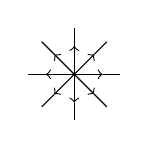
\begin{tikzpicture}[scale=0.45]\foreach \a in {0,45,...,315} \draw[->] (0,0) -- (\a:0.8); \foreach \a in {0,45,...,315} \draw (\a:0.8) -- (\a:1.3);\end{tikzpicture}}
{\begin{tikzpicture}[scale=0.45]\foreach \a in {0,45,...,315} \draw[<-] (0,0) -- (\a:0.8); \foreach \a in {0,45,...,315} \draw (\a:0.8) -- (\a:1.3);\end{tikzpicture}}
{\begin{tikzpicture}[scale=0.45]\foreach \r in {0.45,0.85,1.25} {\draw (0,0) circle (\r); \draw[->] (\r,0.02) -- (\r,-0.02);}\end{tikzpicture}}
{\begin{tikzpicture}[scale=0.45]\foreach \s in {0.5,0.9,1.3} {\draw (0,0) .. controls (\s,1.4*\s) and (2*\s,0.6*\s) .. (2*\s,0) .. controls (2*\s,-0.6*\s) and (\s,-1.4*\s) .. (0,0); \draw (0,0) .. controls (-\s,1.4*\s) and (-2*\s,0.6*\s) .. (-2*\s,0) .. controls (-2*\s,-0.6*\s) and (-\s,-1.4*\s) .. (0,0);} \draw (0,-1.4) -- (0,1.4); \draw[->] (2.6,0.05) -- (2.6,-0.05); \draw[->] (-2.6,0.05) -- (-2.6,-0.05);\end{tikzpicture}}}
\topichead{Magnetic flux}{1}
\numoptsfalse
\QQ{\qsrc{2024}{50}A uniform magnetic field of strength $B = 2\unit{mT}$ exists vertically downwards. These magnetic field lines pass through a closed surface as shown in the figure. The closed surface consists of a hemisphere $S_1$, a right circular cone $S_2$ and a circular surface $S_3$. The magnetic flux through $S_1$ and $S_2$ are respectively
\fig{\begin{tikzpicture}[scale=0.8]
\draw (-1.3,0) arc (180:0:1.3);
\draw (-1.3,0) arc (180:360:1.3 and 0.25); \draw[dashed] (1.3,0) arc (0:180:1.3 and 0.25);
\draw (-1.3,0) -- (0,-2.0) -- (1.3,0);
\fill (0,0) circle (1.2pt); \draw[dashed,->] (0,0) -- (1.3,0);
\node[lbl,right] at (1.4,0) {$R = \dfrac{10}{\sqrt\pi}$};
\foreach \x in {-0.55,0.55} \draw[->] (\x,2.0) -- (\x,-2.3);
\node[lbl] at (1.15,1.15) {$S_1$}; \node[lbl] at (-0.35,0.45) {$S_3$}; \node[lbl] at (1.0,-0.95) {$S_2$};
\node[lbl] at (0.85,-2.1) {$\vec B$};
\end{tikzpicture}}\ntag{A}{143}{leph105}{8}{}{Class XII Part 1 \textperiodcentered{} Ch 5}\nsrc{None found in NEET/AIPMT/AIEEE/JEE papers, 2005--2026 (NCERT concept application)}}
{\opt{$\Phi_{S_1} = -20\unit{\mu Wb}$, $\Phi_{S_2} = +20\unit{\mu Wb}$}{$\Phi_{S_1} = +20\unit{\mu Wb}$, $\Phi_{S_2} = -20\unit{\mu Wb}$}{$\Phi_{S_1} = -40\unit{\mu Wb}$, $\Phi_{S_2} = +40\unit{\mu Wb}$}{$\Phi_{S_1} = +40\unit{\mu Wb}$, $\Phi_{S_2} = -40\unit{\mu Wb}$}}
\topichead{Magnetic materials}{7}
\numoptstrue
\QQ{\qsrc{2026}{37}If a paramagnetic bar is brought near a bar magnet, then it is\ntag{D}{148}{leph105}{13}{}{Class XII Part 1 \textperiodcentered{} Ch 5}}
{\opt{Attracted by both the poles of the bar magnet}{Repelled by both the poles of the bar magnet}{Attracted by the South-pole and repelled by the North-pole of the bar magnet}{Attracted by the North-pole and repelled by the South-pole of the bar magnet}}
\numoptstrue
\QQ{\qsrc{2026}{38}Pick out the WRONG statements about magnetic substances ($\chi$ = magnetic susceptibility) ($\mu_r$ = relative permeability).
\begin{stmts}
\item Substances with $-1\le\chi<0$ are diamagnetic
\item Substances with $\chi\gg1$ are paramagnetic
\item Substances with $\chi\ll1$ are ferromagnetic
\item Substances with $\mu_r\gg1$ are ferromagnetic
\end{stmts}\ntag{D}{147}{leph105}{12}{}{Class XII Part 1 \textperiodcentered{} Ch 5}}
{\opt{I and II}{III and IV}{II and III}{II and IV}}
\numoptstrue
\QQ{\qsrc{2025}{35}Which of the following statements is true in respect of diamagnetic substances?\ntag{D}{147}{leph105}{12}{}{Class XII Part 1 \textperiodcentered{} Ch 5}}
{\opt{Susceptibility is small and negative}{They are feebly attracted by magnets}{Permeability is greater than 1000}{Susceptibility decreases with temperature.}}
\numoptsfalse
\QQ{\qsrc{2020}{30}In a permanent magnet at room temperature\ntag{D}{149}{leph105}{14}{ \textperiodcentered{} Exemplar 5.3}{Class XII Part 1 \textperiodcentered{} Ch 5}}
{\opt{Magnetic moment of each molecule is zero.}{The individual molecules have non-zero magnetic moment which are all perfectly aligned.}{Domains are partially aligned.}{Domains are all perfectly aligned.}}
\numoptsfalse
\QQ{\qsrc{2019}{4}In a permanent magnet at room temperature\ntag{D}{149}{leph105}{14}{ \textperiodcentered{} Exemplar 5.3}{Class XII Part 1 \textperiodcentered{} Ch 5}}
{\opt{magnetic moment of each molecule is zero.}{the individual molecules have non zero magnetic moment which are all perfectly aligned.}{domains are partially aligned.}{domains are all perfectly aligned.}}
\numoptsfalse
\QQ{\qsrc{2018}{32}Needles $N_1$, $N_2$ and $N_3$ are made of a ferromagnetic, a paramagnetic and a diamagnetic substance respectively. A magnet when brought close to them will\ntag{D}{147}{leph105}{12}{}{Class XII Part 1 \textperiodcentered{} Ch 5}}
{\opt{Attract all three of them}{Attract $N_1$ strongly, $N_2$ weakly and repel $N_3$ weakly}{Attract $N_1$ strongly but repel $N_2$ and $N_3$ weakly}{Attract $N_1$ and $N_2$ strongly but repel $N_3$}}
\numoptsfalse
\QQ{\qsrc{2017}{34}The susceptibility of a ferromagnetic substance is\ntag{D}{147}{leph105}{12}{}{Class XII Part 1 \textperiodcentered{} Ch 5}}
{\opt{$\gg1$}{$>1$}{$<1$}{Zero}}
\end{multicols}
\par\needspace{12\baselineskip}\vspace{12pt}
\begin{center}{\pgfornament[width=3.2cm,color=gilt]{87}}\par
{\large\color{navy}\scshape Magnetism and Matter \textperiodcentered{} Answer Key}\end{center}
{\small\setlength{\tabcolsep}{1pt}\renewcommand{\arraystretch}{1.5}
\begin{tabularx}{\linewidth}{@{}*{8}{>{\centering\arraybackslash}X}@{}}\toprule
\textbf{1}\,(D) & \textbf{2}\,(D) & \textbf{3}\,(C) & \textbf{4}\,(A) & \textbf{5}\,(1) & \textbf{6}\,(3) & \textbf{7}\,(1) & \textbf{8}\,(C)\\
\textbf{9}\,(C) & \textbf{10}\,(B) & \textbf{11}\,(A) &  &  &  &  & \\\bottomrule\end{tabularx}}\par\smallskip
{\footnotesize Answers solved by the editor. Option labels are those of the original paper: (1)--(4) for 2016, 2025 and 2026, (A)--(D) for 2017--2024.
}\par
\par\needspace{18\baselineskip}\vspace{14pt}
\begin{center}{\pgfornament[width=3.2cm,color=gilt]{87}}\par
{\large\color{navy}\scshape Chapter Summary \textperiodcentered{} Magnetism and Matter}\end{center}
{\small\setlength{\tabcolsep}{3.5pt}
\begin{tabular*}{\linewidth}{@{\extracolsep{\fill}}l*{11}{c}c@{}}\toprule
Year & 2016 & 2017 & 2018 & 2019 & 2020 & 2021 & 2022 & 2023 & 2024 & 2025 & 2026 & Total\\\midrule
Questions & 0 & 2 & 1 & 1 & 1 & 1 & 0 & 1 & 1 & 1 & 2 & \textbf{11}\\\bottomrule\end{tabular*}}\par\medskip
{\small\textbf{\color{crimson}Topic-wise} (in textbook order)\par\smallskip
\begin{tabularx}{\linewidth}{@{}>{\raggedright\arraybackslash}Xrrrl@{}}\toprule
Topic & Qs & Direct & Years & 2016 $\rightarrow$ 2026\\\midrule
Magnetic dipole and bar magnet & \textbf{2} & 2 & 2 & {\scriptsize {\color{gray!45}16} \textbf{17} {\color{gray!45}18} {\color{gray!45}19} {\color{gray!45}20} {\color{gray!45}21} {\color{gray!45}22} \textbf{23} {\color{gray!45}24} {\color{gray!45}25} {\color{gray!45}26}}\\
Magnetic field lines and Gauss's law for magnetism & \textbf{1} & 1 & 1 & {\scriptsize {\color{gray!45}16} {\color{gray!45}17} {\color{gray!45}18} {\color{gray!45}19} {\color{gray!45}20} \textbf{21} {\color{gray!45}22} {\color{gray!45}23} {\color{gray!45}24} {\color{gray!45}25} {\color{gray!45}26}}\\
Magnetic flux & \textbf{1} & 0 & 1 & {\scriptsize {\color{gray!45}16} {\color{gray!45}17} {\color{gray!45}18} {\color{gray!45}19} {\color{gray!45}20} {\color{gray!45}21} {\color{gray!45}22} {\color{gray!45}23} \textbf{24} {\color{gray!45}25} {\color{gray!45}26}}\\
Magnetic materials & \textbf{7} & 7 & 6 & {\scriptsize {\color{gray!45}16} \textbf{17} \textbf{18} \textbf{19} \textbf{20} {\color{gray!45}21} {\color{gray!45}22} {\color{gray!45}23} {\color{gray!45}24} \textbf{25} \textbf{26}}\\
\bottomrule\end{tabularx}}\par\medskip
\begin{minipage}[t]{0.34\linewidth}{\small\textbf{\color{crimson}Direct vs Applied}\par\smallskip
\begin{tabular}{@{}lrr@{}}\toprule
Direct from NCERT & \textbf{10} & 91\%\\
\quad text, table, figure & 9 &\\
\quad solved Example & 1 &\\
\quad Exercise & 0 &\\
Applied & \textbf{1} & 9\%\\\midrule
Easy / Mod. / Hard & \multicolumn{2}{r}{10 / 1 / 0}\\\bottomrule
\end{tabular}}\end{minipage}\hfill
\begin{minipage}[t]{0.63\linewidth}{\small\textbf{\color{crimson}What to focus on}\par\smallskip
\begin{itemize}[leftmargin=1.1em,itemsep=1pt,topsep=0pt]
\item 11 questions in 11 papers, about 1.0 per paper; rank 20 of 28 chapters by number of questions.
\item Most asked topic: \textbf{Magnetic materials} (7 questions, in 6 of the 11 years).
\item 1 questions are NCERT solved Examples or Exercises: Example 5.3 (Q 3). Work these by hand.
\item NCERT pages that gave three or more questions: page 147 (4 questions). Read these pages line by line.
\item Difficulty: 10 easy, 1 moderate, 0 hard.
\item 1 applied questions.
\end{itemize}}\end{minipage}\par
\chapterpaper{Class XII \textperiodcentered{} Chapter 6}{Electromagnetic Induction}{21 questions \textperiodcentered{} 5 topics \textperiodcentered{} KCET 2016--2026}{cleph106}{XII.6 Electromagnetic Induction}
\begin{multicols}{2}
\topichead{Faraday's law and Lenz's law}{8}
\numoptstrue
\QQ{\qsrc{2026}{41}In Faraday--Henry's experiment, a coil is connected to a galvanometer. For the deflection of pointer in the galvanometer, which of the following statement/s is/are WRONG?\par
The pointer in the galvanometer deflects --
\begin{stmts}[(\alph*)]
\item When the bar magnet is moved towards the stationary coil along its axis
\item When the bar magnet is moved away from the stationary coil along its axis
\item When the coil is moved towards the stationary bar magnet along its axis
\item When the coil and the magnet are moved without relative motion between them
\end{stmts}\ntag{D}{155}{leph106}{2}{}{Class XII Part 1 \textperiodcentered{} Ch 6}}
{\opt{a and b}{b and c}{a, b and c}{Only d}}
\numoptstrue
\QQ{\qsrc{2025}{40}When a bar magnet is pushed towards the coil, along its axis, as shown in the figure, the galvanometer pointer deflects towards X. When this magnet is pulled away from the coil, the galvanometer pointer
\fig{\begin{tikzpicture}[scale=0.7]
\draw (0,0) rectangle (2.6,1.1);
\draw (1.0,1.1) .. controls (0.6,2.0) and (0.4,3.0) .. (1.2,3.1) .. controls (2.0,3.0) and (1.8,2.0) .. (1.4,1.1);
\draw (2.9,1.9) rectangle (4.6,2.5); \node[lbl] at (3.2,2.2) {N}; \node[lbl] at (4.3,2.2) {S};
\draw[fill=parchment] (1.3,0) circle (0.22); \draw[->] (1.3,-0.12) -- (1.3,0.15); \node[lbl,below] at (1.3,-0.25) {G};
\node[lbl] at (-0.3,-0.25) {X$'$}; \node[lbl] at (2.9,-0.25) {X};
\end{tikzpicture}}\ntag{D}{155}{leph106}{2}{}{Class XII Part 1 \textperiodcentered{} Ch 6}}
{\opt{deflects towards X}{deflects towards X$'$}{does not deflect}{oscillates}}
\numoptsfalse
\QQ{\qsrc{2024}{51}In the figure, a conducting ring of certain resistance is falling towards a current carrying straight long conductor. The ring and conductor are in the same plane. Then the
\fig{\begin{tikzpicture}[scale=0.8]
\draw (0.6,1.3) circle (0.5); \node[lbl] at (1.15,1.9) {A};
\draw[->] (-0.2,1.7) -- (-0.2,0.9);
\draw[densely dashed] (-1.6,0) -- (2.6,0);
\fill[gray!70] (-0.9,-0.07) rectangle (1.7,0.07); \node[lbl,above] at (1.3,0.1) {B};
\draw[->] (0.8,-0.35) -- (1.6,-0.35) node[midway,below,lbl]{$I$};
\end{tikzpicture}}\ntag{A}{160}{leph106}{7}{}{Class XII Part 1 \textperiodcentered{} Ch 6}\nsrc{None found in NEET/AIPMT/AIEEE/JEE papers, 2005--2026 (NCERT concept application)}}
{\opt{induced electric current is zero}{induced electric current is anticlockwise}{induced electric current is clockwise}{ring will come to rest}}
\numoptsfalse
\QQ{\qsrc{2024}{52}An induced current of $2\unit{A}$ flows through a coil. The resistance of the coil is $10\unit{\Omega}$. What is the change in magnetic flux associated with the coil in $1\unit{ms}$?\ntag{A}{157}{leph106}{4}{}{Class XII Part 1 \textperiodcentered{} Ch 6}\nsrc{None found in NEET/AIPMT/AIEEE/JEE papers, 2005--2026 (NCERT concept application)}}
{\opt{$0.2\times10^{-2}\unit{Wb}$}{$2\times10^{-2}\unit{Wb}$}{$22\times10^{-2}\unit{Wb}$}{$0.22\times10^{-2}\unit{Wb}$}}
\numoptsfalse
\QQ{\qsrc{2023}{47}A square loop of side $2\unit{cm}$ enters a magnetic field with a constant speed of $2\unit{cm\,s^{-1}}$ as shown. The front edge enters the field at $t = 0\unit{s}$. Which of the following graph correctly depicts the induced emf in the loop? (Take clockwise direction positive)
\fig{\begin{tikzpicture}[scale=0.55]
\draw (0,0) rectangle (1.6,1.6); \node[lbl,above] at (0.8,1.6) {2 cm}; \draw[->] (1.6,0.8) -- (2.4,0.8);
\foreach \x in {2.1,3.0,3.9} \foreach \y in {-0.6,0.1,0.8,1.5,2.2} \node[font=\scriptsize] at (\x,\y) {$\times$};
\node[lbl,right] at (4.1,0.8) {$B = 0.5\unit{T}$};
\draw[<->] (2.1,-1.1) -- (3.9,-1.1) node[midway,below,lbl]{10 cm};
\end{tikzpicture}}\ntag{A}{163}{leph106}{10}{}{Class XII Part 1 \textperiodcentered{} Ch 6}\nsrc{JEE Main 2024 (9 Apr, Shift 2) -- square loop entering a magnetic field at constant speed, induced emf}}
{\optfig{\emfg{\draw (0,0) -- (0,1) -- (1,0) -- (5,0) -- (5,-1) -- (6,0);}}
{\emfg{\draw (0,0) -- (0,-1) -- (1,0) -- (5,0) -- (5,1) -- (6,0);}}
{\emfg{\draw (0,0) -- (0,-1) -- (1,-1) -- (1,0) -- (5,0) -- (5,1) -- (6,1) -- (6,0);}}
{\emfg{\draw (0,0) -- (0,1) -- (1,1) -- (1,0) -- (5,0) -- (5,-1) -- (6,-1) -- (6,0);}}}
\numoptsfalse
\QQ{\qsrc{2022}{54}A magnetic field of flux density $1.0\unit{Wb\,m^{-2}}$ acts normal to a 80 turn coil of $0.01\unit{m^2}$ area. If this coil is removed from the field in 0.2 second, the emf induced in it is\ntag{D}{158}{leph106}{5}{}{Class XII Part 1 \textperiodcentered{} Ch 6}}
{\opt{$0.8\unit{V}$}{$4\unit{V}$}{$5\unit{V}$}{$8\unit{V}$}}
\numoptsfalse
\QQ{\qsrc{2018}{36}The magnetic flux linked with a coil varies as $\phi = 3t^2+4t+9$. The magnitude of the emf induced at $t = 2$ seconds is\ntag{D}{158}{leph106}{5}{}{Class XII Part 1 \textperiodcentered{} Ch 6}}
{\opt{$8\unit{V}$}{$16\unit{V}$}{$32\unit{V}$}{$64\unit{V}$}}
\numoptsfalse
\QQ{\qsrc{2017}{35}A bar magnet is allowed to fall vertically through a copper coil placed in a horizontal plane. The magnet falls with a net acceleration
\fig{\begin{tikzpicture}[scale=0.7]
\draw (-0.25,1.0) rectangle (0.25,2.4); \node[lbl] at (0,2.1) {S}; \node[lbl] at (0,1.3) {N};
\draw[densely dashed,->] (0,1.0) -- (0,0.05); \draw (0,0) ellipse (1.2 and 0.45);
\end{tikzpicture}}\ntag{A}{160}{leph106}{7}{}{Class XII Part 1 \textperiodcentered{} Ch 6}\nsrc{None found in NEET/AIPMT/AIEEE/JEE papers, 2005--2026 (NCERT concept application)}}
{\opt{$= g$}{$> g$}{$< g$}{Zero}}
\topichead{Magnetic flux}{1}
\numoptstrue
\QQ{\qsrc{2025}{41}A square loop of side $2\unit{m}$ lies in the Y-Z plane in a region having a magnetic field $\vec B = (5\hat i+3\hat j-4\hat k)\unit{T}$. The magnitude of magnetic flux through the square loop is\ntag{D}{157}{leph106}{4}{}{Class XII Part 1 \textperiodcentered{} Ch 6}}
{\opt{$10\unit{Wb}$}{$20\unit{Wb}$}{$12\unit{Wb}$}{$16\unit{Wb}$}}
\topichead{Motional emf}{5}
\numoptstrue
\QQ{\qsrc{2026}{42}In the figure shown, the conductor PQ of length $l$ is moved from $x=0$ to $x=b$ and then up to $x=2b$ with a constant velocity $\vec v$. A uniform magnetic field $\vec B$ is perpendicular to the plane of the paper and extends from $x=0$ to $x=b$ and it is zero from $x>b$. The magnitude of emf induced in the conductor is
\fig{\begin{tikzpicture}[scale=0.75]
\foreach \x in {0,0.7,1.4}{\foreach \y in {-0.2,0.6,1.2,1.8,2.6}{\fill (\x,\y) circle (1.3pt);}}
\foreach \y in {-0.2,0.6,1.2,1.8,2.6}{\fill (2.2,\y) circle (1.3pt);}
\node[lbl] at (0.25,2.85) {$\vec B$};
\draw (5.2,2.4) -- (-0.1,2.4) -- (-0.1,0) -- (5.2,0);
\draw (5.2,2.2) -- (0.1,2.2) -- (0.1,0.2) -- (5.2,0.2);
\fill[pattern=north east lines] (1.85,-0.15) rectangle (2.0,2.75);
\node[lbl,above] at (1.92,2.75) {P}; \node[lbl,below] at (1.92,-0.15) {Q};
\draw[<->] (1.6,0.25) -- (1.6,2.15) node[midway,left,lbl,inner sep=1pt]{$l$};
\draw[->] (2.05,1.2) -- (2.8,1.2) node[right,lbl]{$\vec v$};
\draw[densely dashed] (2.2,-0.6) -- (2.2,3.0);
\draw[densely dashed] (4.4,-0.6) -- (4.4,3.0);
\node[lbl] at (0,-0.85) {$x=0$}; \node[lbl] at (2.2,-0.85) {$x=b$}; \node[lbl] at (4.4,-0.85) {$x=2b$};
\end{tikzpicture}}\ntag{D}{162}{leph106}{9}{}{Class XII Part 1 \textperiodcentered{} Ch 6}}
{\opt{$Blx$ ; $0\le x<b$}{Zero ; $0\le x<b$}{$Blv$ ; $0\le x\le b$}{$Blv$ ; $b\le x<2b$}}
\numoptsfalse
\QQ{\qsrc{2023}{46}A metallic rod of length $1\unit{m}$ held along east-west direction is allowed to fall down freely. Given horizontal component of earth's magnetic field $B_H = 3\times10^{-5}\unit{T}$. The emf induced in the rod at an instant $t = 2\unit{s}$ after it is released is (Take $g = 10\unit{m\,s^{-2}}$)\ntag{D}{176}{leph106}{23}{ \textperiodcentered{} Exercise 6.6}{Class XII Part 1 \textperiodcentered{} Ch 6}}
{\opt{$3\times10^{-3}\unit{V}$}{$3\times10^{-4}\unit{V}$}{$6\times10^{-3}\unit{V}$}{$6\times10^{-4}\unit{V}$}}
\numoptsfalse
\QQ{\qsrc{2020}{31}A rod of length $2\unit{m}$ slides with a speed of $5\unit{m\,s^{-1}}$ on a rectangular conducting frame as shown in figure. There exists a uniform magnetic field of $0.04\unit{T}$ perpendicular to the plane of the figure. If the resistance of the rod is $3\unit{\Omega}$. The current through the rod is
\fig{\begin{tikzpicture}[scale=0.6]
\foreach \x in {0,1,...,5} \foreach \y in {0,1,2,3} \node[font=\scriptsize] at (\x,\y) {$\times$};
\draw (3.6,0.6) -- (0.5,0.6) -- (0.5,2.4) -- (3.6,2.4);
\fill[gray!70] (2.9,0.45) rectangle (3.1,2.55);
\draw[<->] (3.35,0.7) -- (3.35,2.3) node[midway,right,lbl]{2 m};
\draw[->] (2.85,1.5) -- (2.1,1.5) node[left,lbl]{$V$};
\end{tikzpicture}}\ntag{A}{163}{leph106}{10}{}{Class XII Part 1 \textperiodcentered{} Ch 6}\nsrc{None found in NEET/AIPMT/AIEEE/JEE papers, 2005--2026 (NCERT concept application)}}
{\opt{$75\unit{mA}$}{$133\unit{mA}$}{$0.75\unit{A}$}{$1.33\unit{A}$}}
\numoptsfalse
\QQ{\qsrc{2019}{28}Consider the situation given in figure. The wire AB is slid on the fixed rails with a constant velocity. If the wire AB is replaced by a semicircular wire, the magnitude of the induced current will
\fig{\begin{tikzpicture}[scale=0.55]
\foreach \x in {0,1,...,6} \foreach \y in {0,1,...,5} \node[font=\scriptsize] at (\x,\y) {$\times$};
\draw (2.5,4.4) -- (6.6,4.4) -- (6.6,0.6) -- (2.5,0.6);
\draw[line width=1pt] (2.5,4.6) -- (2.5,0.4); \node[lbl] at (2.85,4.75) {A}; \node[lbl] at (2.85,0.25) {B};
\draw[->] (2.3,3.0) -- (1.2,3.0) node[above,lbl]{$v$};
\draw[decorate,decoration={zigzag,segment length=3pt,amplitude=2pt}] (6.6,3.2) -- (6.6,1.8);
\end{tikzpicture}}\ntag{A}{163}{leph106}{10}{}{Class XII Part 1 \textperiodcentered{} Ch 6}\nsrc{None found in NEET/AIPMT/AIEEE/JEE papers, 2005--2026 (NCERT concept application)}}
{\opt{increase}{remain same}{decrease}{increase or decrease depending on whether the semicircle bulges towards the resistance or away from it}}
\numoptstrue
\QQ{\qsrc{2016}{38}A wheel with 10 spokes each of length `$L$' m is rotated with a uniform angular velocity `$\omega$' in a plane normal to the magnetic field `$B$'. The emf induced between the axle and the rim of the wheel.\ntag{D}{165}{leph106}{12}{ \textperiodcentered{} Example 6.7}{Class XII Part 1 \textperiodcentered{} Ch 6}}
{\opt{$\dfrac12N\omega BL^2$}{$\dfrac12\omega BL^2$}{$\omega bL^2$}{$N\omega BL^2$}}
\topichead{Self and mutual inductance}{6}
\numoptsfalse
\QQ{\qsrc{2024}{53}A square loop of side length `$a$' is moving away from an infinitely long current carrying conductor at a constant speed `$v$' as shown. Let `$x$' be the instantaneous distance between the long conductor and side AB. The mutual inductance (M) of the square loop -- long conductor pair changes with time ($t$) according to which of the following graphs?
\fig{\begin{tikzpicture}[scale=0.75]
\fill[gray!70] (-0.08,-0.6) rectangle (0.08,2.0); \draw[densely dashed] (0,-1.2) -- (0,-0.6) (0,2.0) -- (0,2.6);
\draw[->] (0.3,1.6) -- (0.3,2.3) node[right,lbl]{$I$};
\draw (1.0,0) rectangle (2.2,1.2);
\node[lbl,left] at (1.0,1.2) {A}; \node[lbl,left] at (1.0,0) {B}; \node[lbl,right] at (2.2,0) {C}; \node[lbl,right] at (2.2,1.2) {D};
\node[lbl,above] at (1.6,1.2) {$a$}; \node[lbl,below] at (1.6,0) {$a$}; \node[lbl,right] at (1.0,0.6) {$a$}; \node[lbl,left] at (2.2,0.6) {$a$};
\draw[->] (1.9,0.9) -- (2.7,0.9) node[right,lbl]{$v$};
\draw[<->] (0.08,-0.2) -- (1.0,-0.2) node[midway,below,lbl]{$x$};
\end{tikzpicture}}\ntag{A}{165}{leph106}{12}{}{Class XII Part 1 \textperiodcentered{} Ch 6}\nsrc{None found in NEET/AIPMT/AIEEE/JEE papers, 2005--2026 (NCERT concept application)}}
{\optfig{\gaxes{$t$}{$M$}{\draw (0.2,1.6) .. controls (0.5,0.5) and (1.0,0.25) .. (1.7,0.15);}}
{\gaxes{$t$}{$M$}{\draw (0,0) -- (1.8,1.1);}}
{\gaxes{$t$}{$M$}{\draw (0,1.1) -- (1.7,1.1);}}
{\gaxes{$t$}{$M$}{\draw (0,1.6) -- (1.2,0);}}}
\numoptsfalse
\QQ{\qsrc{2023}{45}The current in a coil changes from $2\unit{A}$ to $5\unit{A}$ in $0.3\unit{s}$. The magnitude of emf induced in the coil is $1.0\unit{V}$. The value of self-inductance of the coil is\ntag{D}{176}{leph106}{23}{ \textperiodcentered{} Exercise 6.7}{Class XII Part 1 \textperiodcentered{} Ch 6}}
{\opt{$100\unit{mH}$}{$0.1\unit{mH}$}{$10\unit{mH}$}{$1.0\unit{mH}$}}
\numoptsfalse
\QQ{\qsrc{2022}{52}A long solenoid has 500 turns, when a current of $2\unit{A}$ is passed through it, the resulting magnetic flux linked with each turn of the solenoid is $4\times10^{-3}\unit{Wb}$, then self induction of the solenoid is\ntag{D}{168}{leph106}{15}{}{Class XII Part 1 \textperiodcentered{} Ch 6}}
{\opt{2.0 henry}{4.0 henry}{1.0 henry}{2.5 henry}}
\numoptsfalse
\QQ{\qsrc{2021}{36}The current flowing through an inductance coil of self inductance $6\unit{mH}$ at different time instants is as shown. The emf induced between $t = 20\unit{s}$ and $t = 40\unit{s}$ is nearly
\fig{\begin{tikzpicture}[xscale=0.045,yscale=0.42]
\draw[->] (0,0) -- (55,0) node[right,lbl]{$t$ (s)};
\draw[->] (0,0) -- (0,5.2) node[above,lbl]{$I$ (A)};
\draw (0,0) -- (20,4.6) -- (40,3.6) -- (50,0);
\draw (20,0) -- (20,4.6) (40,0) -- (40,3.6);
\foreach \y in {2,4} {\draw (0.8,\y) -- (-0.8,\y) node[left,lbl]{\y};}
\node[lbl,below] at (20,0) {20}; \node[lbl,below] at (40,0) {40};
\end{tikzpicture}}\ntag{D}{168}{leph106}{15}{}{Class XII Part 1 \textperiodcentered{} Ch 6}}
{\opt{$2\times10^{-2}\unit{V}$}{$3\times10^{-2}\unit{V}$}{$4\times10^{-3}\unit{V}$}{$30\times10^{2}\unit{V}$}}
\numoptsfalse
\QQ{\qsrc{2021}{37}The physical quantity which is measured in the unit of $\mathrm{Wb\,A^{-1}}$ is\ntag{D}{165}{leph106}{12}{}{Class XII Part 1 \textperiodcentered{} Ch 6}}
{\opt{Self inductance}{Mutual inductance}{Magnetic flux}{Both (A) and (B)}}
\numoptsfalse
\QQ{\qsrc{2020}{32}The current in a coil of inductance $0.2\unit{H}$ changes from $5\unit{A}$ to $2\unit{A}$ in $0.5\unit{sec}$. The magnitude of the average induced emf in the coil is\ntag{D}{168}{leph106}{15}{}{Class XII Part 1 \textperiodcentered{} Ch 6}}
{\opt{$0.6\unit{V}$}{$1.2\unit{V}$}{$30\unit{V}$}{$0.3\unit{V}$}}
\topichead{Ampere's law and solenoid}{1}
\numoptstrue
\QQ{\qsrc{2016}{37}A long solenoid with 40 turns per cm carries a current of $1\unit{A}$. The magnetic energy stored per unit volume is \rule{1cm}{0.4pt} $\mathrm{J/m^3}$.\ntag{A}{169}{leph106}{16}{}{Class XII Part 1 \textperiodcentered{} Ch 6}\nsrc{None found in NEET/AIPMT/AIEEE/JEE papers, 2005--2026 (NCERT concept application)}}
{\opt{$3.2\pi$}{$32\pi$}{$1.6\pi$}{$6.4\pi$}}
\end{multicols}
\par\needspace{12\baselineskip}\vspace{12pt}
\begin{center}{\pgfornament[width=3.2cm,color=gilt]{87}}\par
{\large\color{navy}\scshape Electromagnetic Induction \textperiodcentered{} Answer Key}\end{center}
{\small\setlength{\tabcolsep}{1pt}\renewcommand{\arraystretch}{1.5}
\begin{tabularx}{\linewidth}{@{}*{8}{>{\centering\arraybackslash}X}@{}}\toprule
\textbf{1}\,(4) & \textbf{2}\,(2) & \textbf{3}\,(C) & \textbf{4}\,(B) & \textbf{5}\,(C) & \textbf{6}\,(B) & \textbf{7}\,(B) & \textbf{8}\,(C)\\
\textbf{9}\,(2) & \textbf{10}\,(3) & \textbf{11}\,(D) & \textbf{12}\,(B) & \textbf{13}\,(B) & \textbf{14}\,(2) & \textbf{15}\,(A) & \textbf{16}\,(A)\\
\textbf{17}\,(C) & \textbf{18}\,(C)$^{*}$ & \textbf{19}\,(D) & \textbf{20}\,(B) & \textbf{21}\,(1) &  &  & \\\bottomrule\end{tabularx}}\par\smallskip
{\footnotesize Answers solved by the editor. Option labels are those of the original paper: (1)--(4) for 2016, 2025 and 2026, (A)--(D) for 2017--2024. $^{*}$: see note.
\par\smallskip\textbf{18.} (KCET 2021 Q36) From the graph the slope is about 0.07\,A/s, giving about $4\times10^{-4}$\,V; option (C) is the nearest.
}\par
\par\needspace{18\baselineskip}\vspace{14pt}
\begin{center}{\pgfornament[width=3.2cm,color=gilt]{87}}\par
{\large\color{navy}\scshape Chapter Summary \textperiodcentered{} Electromagnetic Induction}\end{center}
{\small\setlength{\tabcolsep}{3.5pt}
\begin{tabular*}{\linewidth}{@{\extracolsep{\fill}}l*{11}{c}c@{}}\toprule
Year & 2016 & 2017 & 2018 & 2019 & 2020 & 2021 & 2022 & 2023 & 2024 & 2025 & 2026 & Total\\\midrule
Questions & 2 & 1 & 1 & 1 & 2 & 2 & 2 & 3 & 3 & 2 & 2 & \textbf{21}\\\bottomrule\end{tabular*}}\par\medskip
{\small\textbf{\color{crimson}Topic-wise} (in textbook order)\par\smallskip
\begin{tabularx}{\linewidth}{@{}>{\raggedright\arraybackslash}Xrrrl@{}}\toprule
Topic & Qs & Direct & Years & 2016 $\rightarrow$ 2026\\\midrule
Faraday's law and Lenz's law & \textbf{8} & 4 & 7 & {\scriptsize {\color{gray!45}16} \textbf{17} \textbf{18} {\color{gray!45}19} {\color{gray!45}20} {\color{gray!45}21} \textbf{22} \textbf{23} \textbf{24} \textbf{25} \textbf{26}}\\
Magnetic flux & \textbf{1} & 1 & 1 & {\scriptsize {\color{gray!45}16} {\color{gray!45}17} {\color{gray!45}18} {\color{gray!45}19} {\color{gray!45}20} {\color{gray!45}21} {\color{gray!45}22} {\color{gray!45}23} {\color{gray!45}24} \textbf{25} {\color{gray!45}26}}\\
Motional emf & \textbf{5} & 3 & 5 & {\scriptsize \textbf{16} {\color{gray!45}17} {\color{gray!45}18} \textbf{19} \textbf{20} {\color{gray!45}21} {\color{gray!45}22} \textbf{23} {\color{gray!45}24} {\color{gray!45}25} \textbf{26}}\\
Self and mutual inductance & \textbf{6} & 5 & 5 & {\scriptsize {\color{gray!45}16} {\color{gray!45}17} {\color{gray!45}18} {\color{gray!45}19} \textbf{20} \textbf{21} \textbf{22} \textbf{23} \textbf{24} {\color{gray!45}25} {\color{gray!45}26}}\\
Ampere's law and solenoid & \textbf{1} & 0 & 1 & {\scriptsize \textbf{16} {\color{gray!45}17} {\color{gray!45}18} {\color{gray!45}19} {\color{gray!45}20} {\color{gray!45}21} {\color{gray!45}22} {\color{gray!45}23} {\color{gray!45}24} {\color{gray!45}25} {\color{gray!45}26}}\\
\bottomrule\end{tabularx}}\par\medskip
\begin{minipage}[t]{0.34\linewidth}{\small\textbf{\color{crimson}Direct vs Applied}\par\smallskip
\begin{tabular}{@{}lrr@{}}\toprule
Direct from NCERT & \textbf{13} & 62\%\\
\quad text, table, figure & 10 &\\
\quad solved Example & 1 &\\
\quad Exercise & 2 &\\
Applied & \textbf{8} & 38\%\\\midrule
Easy / Mod. / Hard & \multicolumn{2}{r}{14 / 7 / 0}\\\bottomrule
\end{tabular}}\end{minipage}\hfill
\begin{minipage}[t]{0.63\linewidth}{\small\textbf{\color{crimson}What to focus on}\par\smallskip
\begin{itemize}[leftmargin=1.1em,itemsep=1pt,topsep=0pt]
\item 21 questions in 11 papers, about 1.9 per paper; rank 10 of 28 chapters by number of questions.
\item Most asked topic: \textbf{Faraday's law and Lenz's law} (8 questions, in 7 of the 11 years).
\item 3 questions are NCERT solved Examples or Exercises: Example 6.7 (Q 14), Exercise 6.6 (Q 11), Exercise 6.7 (Q 16). Work these by hand.
\item NCERT pages that gave three or more questions: page 163 (3 questions), page 165 (3 questions), page 168 (3 questions). Read these pages line by line.
\item Difficulty: 14 easy, 7 moderate, 0 hard.
\item 8 applied questions; 1 closely resemble a NEET/JEE/AIEEE question (marked in their tags).
\end{itemize}}\end{minipage}\par
\chapterpaper{Class XII \textperiodcentered{} Chapter 7}{Alternating Current}{31 questions \textperiodcentered{} 4 topics \textperiodcentered{} KCET 2016--2026}{cleph107}{XII.7 Alternating Current}
\begin{multicols}{2}
\topichead{AC power and rms values}{11}
\numoptstrue
\QQ{\qsrc{2026}{44}A light bulb rated $100\unit{W}$ is connected to an AC source of $220\unit{V}$, $50\unit{Hz}$. The rms current through the bulb is\ntag{D}{180}{leph107}{4}{ \textperiodcentered{} Example 7.1}{Class XII Part 1 \textperiodcentered{} Ch 7}}
{\opt{$0.454\unit{A}$}{$0.545\unit{A}$}{$2.20\unit{A}$}{$0.22\unit{A}$}}
\numoptstrue
\QQ{\qsrc{2025}{42}In domestic electric mains supply, the voltage and the current are\ntag{D}{177}{leph107}{1}{}{Class XII Part 1 \textperiodcentered{} Ch 7}}
{\opt{AC voltage and AC current}{AC voltage and DC current}{DC voltage and DC current}{DC voltage and AC current}}
\numoptstrue
\QQ{\qsrc{2025}{43}A sinusoidal voltage produced by an AC generator at any instant $t$ is given by an equation $V = 311\sin314t$. The rms value of voltage and frequency are respectively\ntag{D}{180}{leph107}{4}{}{Class XII Part 1 \textperiodcentered{} Ch 7}}
{\opt{$200\unit{V}$, $100\unit{Hz}$}{$200\unit{V}$, $50\unit{Hz}$}{$220\unit{V}$, $100\unit{Hz}$}{$220\unit{V}$, $50\unit{Hz}$}}
\numoptsfalse
\QQ{\qsrc{2022}{50}An alternating current is given by $i = i_1\sin\omega t+i_2\cos\omega t$. The r.m.s.\ current is given by\ntag{A}{179}{leph107}{3}{}{Class XII Part 1 \textperiodcentered{} Ch 7}\nsrc{None found in NEET/AIPMT/AIEEE/JEE papers, 2005--2026 (NCERT concept application)}}
{\opt{$\sqrt{\dfrac{i_1^2+i_2^2}{2}}$}{$\dfrac{i_1+i_2}{\sqrt2}$}{$\sqrt{\dfrac{i_1^2+i_2^2}{\sqrt2}}$}{$\dfrac{i_1-i_2}{\sqrt2}$}}
\numoptsfalse
\QQ{\qsrc{2019}{29}The frequency of an alternating current is $50\unit{Hz}$. What is the minimum time taken by current to reach its peak value from rms value?\ntag{A}{180}{leph107}{4}{}{Class XII Part 1 \textperiodcentered{} Ch 7}\nsrc{None found in NEET/AIPMT/AIEEE/JEE papers, 2005--2026 (NCERT concept application)}}
{\opt{$5\times10^{-3}\unit{s}$}{$2.5\times10^{-3}\unit{s}$}{$0.02\unit{s}$}{$10\times10^{-3}\unit{s}$}}
\numoptsfalse
\QQ{\qsrc{2019}{36}An inductor of inductance L and resistor R are joined together in series and connected by a source of frequency $\omega$. The power dissipated in the circuit is\ntag{A}{191}{leph107}{15}{}{Class XII Part 1 \textperiodcentered{} Ch 7}\nsrc{None found in NEET/AIPMT/AIEEE/JEE papers, 2005--2026 (NCERT concept application)}}
{\opt{$\dfrac{R^2+\omega^2L^2}{V}$}{$\dfrac{V^2R}{R^2+\omega^2L^2}$}{$\dfrac{V}{R^2+\omega^2L^2}$}{$\dfrac{V^2R}{\sqrt{R^2+\omega^2L^2}}$}}
\numoptsfalse
\QQ{\qsrc{2018}{37}A $100\unit{W}$ bulb is connected to an AC source of $220\unit{V}$, $50\unit{Hz}$. Then the current flowing through the bulb is\ntag{D}{180}{leph107}{4}{ \textperiodcentered{} Example 7.1}{Class XII Part 1 \textperiodcentered{} Ch 7}}
{\opt{$\dfrac5{11}\unit{A}$}{$\dfrac12\unit{A}$}{$2\unit{A}$}{$\dfrac34\unit{A}$}}
\numoptsfalse
\QQ{\qsrc{2018}{38}In the series LCR circuit, the power dissipation is through\ntag{D}{191}{leph107}{15}{}{Class XII Part 1 \textperiodcentered{} Ch 7}}
{\opt{R}{L}{C}{Both L and C}}
\numoptsfalse
\QQ{\qsrc{2018}{39}In Karnataka, the normal domestic power supply AC is $220\unit{V}$, $50\unit{Hz}$. Here $220\unit{V}$ and $50\unit{Hz}$ refer to\ntag{D}{180}{leph107}{4}{}{Class XII Part 1 \textperiodcentered{} Ch 7}}
{\opt{Peak value of voltage and frequency}{rms value of voltage and frequency}{Mean value of voltage and frequency}{Peak value of voltage and angular frequency}}
\numoptstrue
\QQ{\qsrc{2016}{39}The rms value of current in a $50\unit{Hz}$ AC circuit is $6\unit{A}$. The average value of AC current over a cycle is\ntag{D}{178}{leph107}{2}{}{Class XII Part 1 \textperiodcentered{} Ch 7}}
{\opt{$6\sqrt2$}{$\dfrac{3}{\pi\sqrt2}$}{Zero}{$\dfrac{6}{\pi\sqrt2}$}}
\numoptstrue
\QQ{\qsrc{2016}{42}In a series L.C.R.\ circuit an alternating emf ($v$) and current ($i$) are given by the equation $v = v_0\sin\omega t$, $i = i_0\sin\left(\omega t+\dfrac\pi3\right)$. The average power dissipated in the circuit over a cycle of AC is\ntag{D}{191}{leph107}{15}{}{Class XII Part 1 \textperiodcentered{} Ch 7}}
{\opt{$\dfrac{v_0i_0}{2}$}{$\dfrac{v_0i_0}{4}$}{$\dfrac{\sqrt3}{2}v_0i_0$}{Zero}}
\topichead{AC circuits (reactance, LCR, phase)}{16}
\numoptstrue
\QQ{\qsrc{2026}{43}In a circuit containing a pure resistor connected to an AC source,\ntag{D}{178}{leph107}{2}{}{Class XII Part 1 \textperiodcentered{} Ch 7}}
{\opt{Voltage leads the current by $90^\circ$}{Current leads the voltage by $90^\circ$}{Voltage and current are in same phase with each other}{Current leads the voltage by $180^\circ$}}
\numoptstrue
\QQ{\qsrc{2025}{44}A series LCR circuit containing an AC source of $100\unit{V}$ has an inductor and a capacitor of reactances $24\unit{\Omega}$ and $16\unit{\Omega}$ respectively. If a resistance of $6\unit{\Omega}$ is connected in series, then the potential difference across the series combination of inductor and capacitor only is\ntag{A}{186}{leph107}{10}{}{Class XII Part 1 \textperiodcentered{} Ch 7}\nsrc{None found in NEET/AIPMT/AIEEE/JEE papers, 2005--2026 (NCERT concept application)}}
{\opt{$40\unit{V}$}{$80\unit{V}$}{$400\unit{V}$}{$8\unit{V}$}}
\numoptsfalse
\QQ{\qsrc{2024}{55}In an LCR series circuit, the value of only capacitance $C$ is varied. The resulting variation of resonance frequency ($f_0$) as a function of $C$ can be represented as\ntag{D}{189}{leph107}{13}{}{Class XII Part 1 \textperiodcentered{} Ch 7}}
{\optfig{\gaxes{$C$}{$f_0$}{\draw (0.1,0.1) .. controls (0.6,0.1) and (0.6,1.5) .. (0.9,1.5) .. controls (1.2,1.5) and (1.2,0.1) .. (1.7,0.1);}}
{\gaxes{$C$}{$f_0$}{\draw (0,0) -- (1.6,1.6);}}
{\gaxes{$C$}{$f_0$}{\draw[domain=0.12:1.9,samples=40] plot (\x,{0.5/sqrt(\x)-0.15});}}
{\gaxes{$C$}{$f_0$}{\draw[domain=0:1.9,samples=40] plot (\x,{1.2*sqrt(\x)});}}}
\numoptsfalse
\QQ{\qsrc{2024}{56}The figure shows variation of $R$, $X_L$ and $X_C$ with frequency `$f$' in a series LCR circuit. Then for what frequency point is the circuit capacitive?
\fig{\begin{tikzpicture}[scale=0.8]
\draw[->] (0,0) -- (4.3,0) node[right,lbl]{$f$};
\draw[->] (0,0) -- (0,2.8);
\draw (0,0.9) -- (3.6,0.9) node[above,lbl]{$R$};
\draw (0,0) -- (2.3,2.4) node[above,lbl]{$X_L$};
\draw[domain=0.3:2.8,samples=40] plot (\x,{0.75/\x+0.15}) ; \node[lbl,above] at (0.32,2.5) {$X_C$};
\draw[densely dashed] (0.86,0.9) -- (0.86,0) node[below,lbl]{A};
\draw[densely dashed] (1.12,1.17) -- (1.12,0) node[below,lbl]{B};
\draw[densely dashed] (1.25,0.9) -- (1.25,0) node[below,lbl]{C};
\draw[densely dashed] (2.0,0.53) -- (2.0,0) node[below,lbl]{D};
\end{tikzpicture}}\ntag{D}{188}{leph107}{12}{}{Class XII Part 1 \textperiodcentered{} Ch 7}}
{\opt{B}{D}{A}{C}}
\numoptsfalse
\QQ{\qsrc{2023}{43}In series LCR circuit at resonance, the phase difference between voltage and current is\ntag{D}{191}{leph107}{15}{}{Class XII Part 1 \textperiodcentered{} Ch 7}}
{\opt{$\pi$}{$\dfrac\pi4$}{$\dfrac\pi2$}{zero}}
\numoptsfalse
\QQ{\qsrc{2022}{57}A series resonant ac circuit contains a capacitance $10^{-6}\unit{F}$ and an inductor of $10^{-4}\unit{H}$. The frequency of electrical oscillations will be\ntag{D}{189}{leph107}{13}{}{Class XII Part 1 \textperiodcentered{} Ch 7}}
{\opt{$\dfrac{10^5}{2\pi}\unit{Hz}$}{$10^5\unit{Hz}$}{$\dfrac{10}{2\pi}\unit{Hz}$}{$10\unit{Hz}$}}
\numoptsfalse
\QQ{\qsrc{2022}{58}In a series LCR circuit $R = 300\unit{\Omega}$, $L = 0.9\unit{H}$, $C = 2.0\unit{\mu F}$ and $\omega = 1000\unit{rad/sec}$, then impedance of the circuit is\ntag{D}{187}{leph107}{11}{}{Class XII Part 1 \textperiodcentered{} Ch 7}}
{\opt{$500\unit{\Omega}$}{$1300\unit{\Omega}$}{$400\unit{\Omega}$}{$900\unit{\Omega}$}}
\numoptsfalse
\QQ{\qsrc{2021}{38}What will be the reading in the voltmeter and ammeter of the circuit shown?
\fig{\begin{circuitikz}[scale=0.6,transform shape,font=\Large]
\draw (0,3) -- (3,3) to[rmeter,t=A] (6,3) to[sV,l=$90\,\mathrm{V}$] (6,0) to[R,l={$R=45\,\Omega$}] (3,0) to[L,l={$X_L=4\,\Omega$}] (0,0) to[C,l={$X_C=4\,\Omega$}] (0,3);
\draw (3,3) to[rmeter,t=V] (3,0);
\end{circuitikz}}\ntag{A}{188}{leph107}{12}{}{Class XII Part 1 \textperiodcentered{} Ch 7}\nsrc{None found in NEET/AIPMT/AIEEE/JEE papers, 2005--2026 (NCERT concept application)}}
{\opt{90\,V, 2\,A}{0\,V, 2\,A}{90\,V, 1\,A}{0\,V, 1\,A}}
\numoptsfalse
\QQ{\qsrc{2020}{33}In the given circuit the peak voltages across C, L and R are $30\unit{V}$, $110\unit{V}$ and $60\unit{V}$ respectively. The rms value of the applied voltage is
\fig{\begin{circuitikz}[scale=0.62,transform shape,font=\Large]
\draw (0,2) to[C,l=C] (2,2) to[L,l=L] (4.2,2) to[R,l=R] (6.2,2) -- (6.2,0) to[sV] (0,0) -- (0,2);
\draw[<->] (0.2,1.2) -- (1.8,1.2) node[midway,below]{30 V}; \draw[<->] (2.1,1.2) -- (4.1,1.2) node[midway,below]{110 V}; \draw[<->] (4.3,1.2) -- (6.0,1.2) node[midway,below]{60 V};
\end{circuitikz}}\ntag{A}{187}{leph107}{11}{}{Class XII Part 1 \textperiodcentered{} Ch 7}\nsrc{None found in NEET/AIPMT/AIEEE/JEE papers, 2005--2026 (NCERT concept application)}}
{\opt{$100\unit{V}$}{$200\unit{V}$}{$70.7\unit{V}$}{$141\unit{V}$}}
\numoptsfalse
\QQ{\qsrc{2020}{34}The power factor of R-L circuit is $\dfrac1{\sqrt3}$. If the inductive reactance is $2\unit{\Omega}$. The value of resistance is\ntag{A}{191}{leph107}{15}{}{Class XII Part 1 \textperiodcentered{} Ch 7}\nsrc{None found in NEET/AIPMT/AIEEE/JEE papers, 2005--2026 (NCERT concept application)}}
{\opt{$2\unit{\Omega}$}{$\sqrt2\unit{\Omega}$}{$0.5\unit{\Omega}$}{$\dfrac1{\sqrt2}\unit{\Omega}$}}
\numoptsfalse
\QQ{\qsrc{2020}{35}In the given circuit, the resonant frequency is
\fig{\begin{circuitikz}[scale=0.62,transform shape,font=\Large]
\draw (0,0) to[L,l=$0.5\,\mathrm{mH}$] (0,2.2) -- (3.6,2.2) to[C,l=$20\,\mu\mathrm{F}$] (3.6,0) -- (0,0);
\end{circuitikz}}\ntag{D}{189}{leph107}{13}{}{Class XII Part 1 \textperiodcentered{} Ch 7}}
{\opt{$15.92\unit{Hz}$}{$159.2\unit{Hz}$}{$1592\unit{Hz}$}{$15910\unit{Hz}$}}
\numoptsfalse
\QQ{\qsrc{2019}{30}The readings of ammeter and voltmeter in the following circuit are respectively
\fig{\begin{circuitikz}[scale=0.6,transform shape,font=\Large]
\draw (0,2.4) to[L,l=L,a={$V_L=50\,\mathrm V$}] (2.6,2.4) to[C,l=C,a={$V_C=50\,\mathrm V$}] (4.8,2.4) to[R,l={$R=100\,\Omega$}] (7.2,2.4) -- (7.2,0) to[sV,l={220 V, 50 Hz}] (0,0) to[rmeter,t=A] (0,2.4);
\draw (4.8,2.4) -- (4.8,1.4) to[rmeter,t=V] (7.2,1.4) -- (7.2,2.4);
\end{circuitikz}}\ntag{A}{188}{leph107}{12}{}{Class XII Part 1 \textperiodcentered{} Ch 7}\nsrc{None found in NEET/AIPMT/AIEEE/JEE papers, 2005--2026 (NCERT concept application)}}
{\opt{1.2\,A, 120\,V}{1.5\,A, 100\,V}{2.7\,A, 220\,V}{2.2\,A, 220\,V}}
\numoptsfalse
\QQ{\qsrc{2018}{35}Which of the following, represents the variation of inductive reactance ($X_L$) with the frequency of voltage source ($\nu$)?\ntag{D}{182}{leph107}{6}{}{Class XII Part 1 \textperiodcentered{} Ch 7}}
{\optfig{\gaxes{$\nu$}{$X_L$}{\draw (0,0) -- (1.5,1.5);}}{\gaxes{$\nu$}{$X_L$}{\draw (0.1,0.1) .. controls (0.9,0.15) and (1.4,0.6) .. (1.6,1.5);}}{\gaxes{$\nu$}{$X_L$}{\draw (0.1,0.1) .. controls (0.2,1.0) and (0.7,1.4) .. (1.6,1.5);}}{\gaxes{$\nu$}{$X_L$}{\draw (0.15,1.6) .. controls (0.3,0.4) and (0.8,0.2) .. (1.7,0.15);}}}
\numoptsfalse
\QQ{\qsrc{2017}{40}A coil of inductive reactance $1/\sqrt3\unit{\Omega}$ and resistance $1\unit{\Omega}$ is connected to a $200\unit{V}$, $50\unit{Hz}$ A.C.\ supply. The time lag between maximum voltage and current is\ntag{A}{188}{leph107}{12}{}{Class XII Part 1 \textperiodcentered{} Ch 7}\nsrc{None found in NEET/AIPMT/AIEEE/JEE papers, 2005--2026 (NCERT concept application)}}
{\opt{$\dfrac1{300}\unit{s}$}{$\dfrac1{600}\unit{s}$}{$\dfrac1{500}\unit{s}$}{$\dfrac1{200}\unit{s}$}}
\numoptstrue
\QQ{\qsrc{2016}{40}A capacitor of capacitance $10\unit{\mu F}$ is connected to an AC source and an AC Ammeter. If the source voltage varies as $V = 50\sqrt2\sin100t$, the reading of the ammeter is\ntag{D}{185}{leph107}{9}{}{Class XII Part 1 \textperiodcentered{} Ch 7}}
{\opt{$50\unit{mA}$}{$70.7\unit{mA}$}{$5.0\unit{mA}$}{$7.07\unit{mA}$}}
\numoptstrue
\QQ{\qsrc{2016}{41}In a series L.C.R circuit, the potential drop across L, C and R respectively are $40\unit{V}$, $120\unit{V}$ and $60\unit{V}$. Then the source voltage is\ntag{D}{187}{leph107}{11}{}{Class XII Part 1 \textperiodcentered{} Ch 7}}
{\opt{$220\unit{V}$}{$160\unit{V}$}{$180\unit{V}$}{$100\unit{V}$}}
\topichead{Self and mutual inductance}{1}
\numoptsfalse
\QQ{\qsrc{2017}{38}In the A.C.\ circuit shown, keeping `K' pressed, if an iron rod is inserted into the coil, the bulb in the circuit,
\fig{\begin{circuitikz}[scale=0.6,transform shape,font=\Large]
\draw (0,0) to[sV,l_=A.C] (0,2.2) to[lamp,l=Bulb] (2.4,2.2) to[L,l=Coil] (5,2.2) -- (6,2.2) -- (6,0) to[push button,l_=K] (3.6,0) -- (0,0);
\fill[pattern=north east lines] (5.4,2.6) rectangle (7.2,2.85); \node at (6.3,3.2) {Rod};
\end{circuitikz}}\ntag{D}{186}{leph107}{10}{ \textperiodcentered{} Example 7.5}{Class XII Part 1 \textperiodcentered{} Ch 7}}
{\opt{glows more brightly}{glows less brightly}{glows with same brightness (as before the rod is inserted)}{gets damaged}}
\topichead{Transformer and power transmission}{3}
\numoptsfalse
\QQ{\qsrc{2023}{44}An ideal transformer has a turns ratio of 10. When the primary is connected to $220\unit{V}$, $50\unit{Hz}$ ac source, the power output is\ntag{D}{195}{leph107}{19}{}{Class XII Part 1 \textperiodcentered{} Ch 7}}
{\opt{$\frac{1}{10}$th the power input}{equal to power input}{zero}{10 times the power input}}
\numoptsfalse
\QQ{\qsrc{2018}{40}A step-up transformer operates on a $230\unit{V}$ line and a load current of $2\unit{A}$. The ratio of primary and secondary windings is 1:25. Then the current in the primary is\ntag{D}{195}{leph107}{19}{}{Class XII Part 1 \textperiodcentered{} Ch 7}}
{\opt{$25\unit{A}$}{$50\unit{A}$}{$15\unit{A}$}{$12.5\unit{A}$}}
\numoptsfalse
\QQ{\qsrc{2017}{39}The output of a step down transformer is measured to be $48\unit{V}$ when connected to a $12\unit{W}$ bulb. The value of peak current is\ntag{A}{195}{leph107}{19}{}{Class XII Part 1 \textperiodcentered{} Ch 7}\nsrc{None found in NEET/AIPMT/AIEEE/JEE papers, 2005--2026 (NCERT concept application)}}
{\opt{$\dfrac1{\sqrt2}\unit{A}$}{$\sqrt2\unit{A}$}{$\dfrac1{2\sqrt2}\unit{A}$}{$\dfrac14\unit{A}$}}
\end{multicols}
\par\needspace{12\baselineskip}\vspace{12pt}
\begin{center}{\pgfornament[width=3.2cm,color=gilt]{87}}\par
{\large\color{navy}\scshape Alternating Current \textperiodcentered{} Answer Key}\end{center}
{\small\setlength{\tabcolsep}{1pt}\renewcommand{\arraystretch}{1.5}
\begin{tabularx}{\linewidth}{@{}*{8}{>{\centering\arraybackslash}X}@{}}\toprule
\textbf{1}\,(1) & \textbf{2}\,(1) & \textbf{3}\,(4) & \textbf{4}\,(A) & \textbf{5}\,(B) & \textbf{6}\,(B) & \textbf{7}\,(A) & \textbf{8}\,(A)\\
\textbf{9}\,(B) & \textbf{10}\,(3) & \textbf{11}\,(2) & \textbf{12}\,(3) & \textbf{13}\,(2) & \textbf{14}\,(C) & \textbf{15}\,(C) & \textbf{16}\,(D)\\
\textbf{17}\,(A) & \textbf{18}\,(A) & \textbf{19}\,(B) & \textbf{20}\,(C) & \textbf{21}\,(B) & \textbf{22}\,(C) & \textbf{23}\,(D) & \textbf{24}\,(A)\\
\textbf{25}\,(B) & \textbf{26}\,(1) & \textbf{27}\,(4) & \textbf{28}\,(B) & \textbf{29}\,(B) & \textbf{30}\,(B) & \textbf{31}\,(C) & \\\bottomrule\end{tabularx}}\par\smallskip
{\footnotesize Answers solved by the editor. Option labels are those of the original paper: (1)--(4) for 2016, 2025 and 2026, (A)--(D) for 2017--2024.
}\par
\par\needspace{18\baselineskip}\vspace{14pt}
\begin{center}{\pgfornament[width=3.2cm,color=gilt]{87}}\par
{\large\color{navy}\scshape Chapter Summary \textperiodcentered{} Alternating Current}\end{center}
{\small\setlength{\tabcolsep}{3.5pt}
\begin{tabular*}{\linewidth}{@{\extracolsep{\fill}}l*{11}{c}c@{}}\toprule
Year & 2016 & 2017 & 2018 & 2019 & 2020 & 2021 & 2022 & 2023 & 2024 & 2025 & 2026 & Total\\\midrule
Questions & 4 & 3 & 5 & 3 & 3 & 1 & 3 & 2 & 2 & 3 & 2 & \textbf{31}\\\bottomrule\end{tabular*}}\par\medskip
{\small\textbf{\color{crimson}Topic-wise} (in textbook order)\par\smallskip
\begin{tabularx}{\linewidth}{@{}>{\raggedright\arraybackslash}Xrrrl@{}}\toprule
Topic & Qs & Direct & Years & 2016 $\rightarrow$ 2026\\\midrule
AC power and rms values & \textbf{11} & 8 & 6 & {\scriptsize \textbf{16} {\color{gray!45}17} \textbf{18} \textbf{19} {\color{gray!45}20} {\color{gray!45}21} \textbf{22} {\color{gray!45}23} {\color{gray!45}24} \textbf{25} \textbf{26}}\\
AC circuits (reactance, LCR, phase) & \textbf{16} & 10 & 11 & {\scriptsize \textbf{16} \textbf{17} \textbf{18} \textbf{19} \textbf{20} \textbf{21} \textbf{22} \textbf{23} \textbf{24} \textbf{25} \textbf{26}}\\
Self and mutual inductance & \textbf{1} & 1 & 1 & {\scriptsize {\color{gray!45}16} \textbf{17} {\color{gray!45}18} {\color{gray!45}19} {\color{gray!45}20} {\color{gray!45}21} {\color{gray!45}22} {\color{gray!45}23} {\color{gray!45}24} {\color{gray!45}25} {\color{gray!45}26}}\\
Transformer and power transmission & \textbf{3} & 2 & 3 & {\scriptsize {\color{gray!45}16} \textbf{17} \textbf{18} {\color{gray!45}19} {\color{gray!45}20} {\color{gray!45}21} {\color{gray!45}22} \textbf{23} {\color{gray!45}24} {\color{gray!45}25} {\color{gray!45}26}}\\
\bottomrule\end{tabularx}}\par\medskip
\begin{minipage}[t]{0.34\linewidth}{\small\textbf{\color{crimson}Direct vs Applied}\par\smallskip
\begin{tabular}{@{}lrr@{}}\toprule
Direct from NCERT & \textbf{21} & 68\%\\
\quad text, table, figure & 18 &\\
\quad solved Example & 3 &\\
\quad Exercise & 0 &\\
Applied & \textbf{10} & 32\%\\\midrule
Easy / Mod. / Hard & \multicolumn{2}{r}{22 / 9 / 0}\\\bottomrule
\end{tabular}}\end{minipage}\hfill
\begin{minipage}[t]{0.63\linewidth}{\small\textbf{\color{crimson}What to focus on}\par\smallskip
\begin{itemize}[leftmargin=1.1em,itemsep=1pt,topsep=0pt]
\item 31 questions in 11 papers, about 2.8 per paper; rank 6 of 28 chapters by number of questions.
\item Most asked topic: \textbf{AC circuits (reactance, LCR, phase)} (16 questions, in 11 of the 11 years).
\item Asked in 8 or more of the 11 years: AC circuits (reactance, LCR, phase).
\item 3 questions are NCERT solved Examples or Exercises: Example 7.1 (Q 1), Example 7.1 (Q 7), Example 7.5 (Q 28). Work these by hand.
\item NCERT pages that gave three or more questions: page 180 (5 questions), page 191 (5 questions), page 188 (4 questions), page 189 (3 questions), page 187 (3 questions), page 195 (3 questions). Read these pages line by line.
\item Difficulty: 22 easy, 9 moderate, 0 hard.
\item 10 applied questions.
\end{itemize}}\end{minipage}\par
\chapterpaper{Class XII \textperiodcentered{} Chapter 8}{Electromagnetic Waves}{10 questions \textperiodcentered{} 3 topics \textperiodcentered{} KCET 2016--2026}{cleph108}{XII.8 Electromagnetic Waves}
\begin{multicols}{2}
\topichead{Displacement current and Maxwell's equations}{1}
\numoptstrue
\QQ{\qsrc{2026}{46}Match the following Maxwell's equations: (The symbols used here have their usual meanings)\par\smallskip
\textit{List-I}\par
\begin{tabular}{@{}ll@{}}
(a) & Gauss' law for electrostatics\\ (b) & Gauss' law for magnetism\\
(c) & Faraday's law\\ (d) & Ampere--Maxwell's law
\end{tabular}\par\smallskip
\textit{List-II}\par
\begin{tabular}{@{}ll@{}}
(i) & $\oint\vec E\cdot d\vec A = \dfrac{Q}{\varepsilon_0}$\\[8pt]
(ii) & $\oint\vec B\cdot d\vec l = \mu_0\left[i_c+\varepsilon_0\dfrac{d\phi_E}{dt}\right]$\\[8pt]
(iii) & $\oint\vec B\cdot d\vec A = 0$\\[4pt]
(iv) & $\oint\vec E\cdot d\vec l = -\dfrac{d\phi_B}{dt}$
\end{tabular}\par\smallskip
Codes:\ntag{D}{205}{leph108}{5}{}{Class XII Part 1 \textperiodcentered{} Ch 8}}
{\opt{a--i, b--iii, c--iv, d--ii}{a--ii, b--iii, c--i, d--iv}{a--i, b--ii, c--iii, d--iv}{a--ii, b--iii, c--iv, d--i}}
\topichead{Electromagnetic waves (nature, E/B = c)}{5}
\numoptsfalse
\QQ{\qsrc{2023}{53}The ratio of the magnitudes of electric field to the magnetic field of an electromagnetic wave is of the order of\ntag{D}{207}{leph108}{7}{}{Class XII Part 1 \textperiodcentered{} Ch 8}}
{\opt{$10^5\unit{m\,s^{-1}}$}{$10^{-5}\unit{m\,s^{-1}}$}{$10^8\unit{m\,s^{-1}}$}{$10^{-8}\unit{m\,s^{-1}}$}}
\numoptsfalse
\QQ{\qsrc{2021}{41}Suppose that the electric field amplitude of electromagnetic wave is $E_0 = 120\unit{N\,C^{-1}}$ and its frequency is $f = 50\unit{MHz}$. Then which of the following value is incorrectly computed?\ntag{D}{214}{leph108}{14}{ \textperiodcentered{} Exercise 8.8}{Class XII Part 1 \textperiodcentered{} Ch 8}}
{\opt{Magnetic field amplitude is $400\unit{nT}$.}{Angular frequency of EM wave is $\pi\times10^8\unit{rad/s}$}{Propagation constant (angular wave number) is $2.1\unit{rad/m}$}{Wavelength of the EM wave is $6\unit{m}$.}}
\numoptsfalse
\QQ{\qsrc{2021}{42}The source of electromagnetic waves can be a charge.\ntag{D}{205}{leph108}{5}{}{Class XII Part 1 \textperiodcentered{} Ch 8}}
{\opt{Moving with a constant velocity}{Moving in a circular orbit.}{At rest}{Moving parallel to the magnetic field}}
\numoptsfalse
\QQ{\qsrc{2019}{37}An electromagnetic wave is travelling in $x$-direction with electric field vector given by, $\vec E_y = E_0\sin(kx-\omega t)\,\hat j$. The correct expression for magnetic field vector is\ntag{D}{206}{leph108}{6}{}{Class XII Part 1 \textperiodcentered{} Ch 8}}
{\opt{$\vec B_y = E_0C\sin(kx-\omega t)\,\hat j$}{$\vec B_z = E_0C\sin(kx-\omega t)\,\hat k$}{$\vec B_y = \dfrac{E_0}{C}\sin(kx-\omega t)\,\hat j$}{$\vec B_z = \dfrac{E_0}{C}\sin(kx-\omega t)\,\hat k$}}
\numoptsfalse
\QQ{\qsrc{2017}{41}If $\vec E$ and $\vec B$ represent electric and magnetic field vectors of an electromagnetic wave, the direction of propagation of the wave is along\ntag{D}{206}{leph108}{6}{}{Class XII Part 1 \textperiodcentered{} Ch 8}}
{\opt{$\vec E$}{$\vec B$}{$\vec E\times\vec B$}{$\vec B\times\vec E$}}
\topichead{Electromagnetic spectrum}{4}
\numoptstrue
\QQ{\qsrc{2026}{51}What range of electromagnetic spectrum is considered as light?\ntag{D}{210}{leph108}{10}{}{Class XII Part 1 \textperiodcentered{} Ch 8}}
{\opt{$1\unit{mm}$ to $700\unit{nm}$}{$400\unit{nm}$ to $1\unit{nm}$}{$400\unit{nm}$ to $700\unit{nm}$}{$1\unit{nm}$ to $10^{-3}\unit{nm}$}}
\numoptstrue
\QQ{\qsrc{2025}{45}Match the following types of waves with their wavelength ranges\par\smallskip
\begin{tabular}{@{}ll@{\quad}ll@{}}
\multicolumn{2}{@{}l}{\textit{Waves}} & \multicolumn{2}{l}{\textit{Wavelength ranges}}\\[2pt]
i. & Microwave & (a) & $700\unit{nm}$ to $400\unit{nm}$\\
ii. & Visible light & (b) & $1\unit{nm}$ to $10^{-3}\unit{nm}$\\
iii. & Ultraviolet & (c) & $0.1\unit{m}$ to $1\unit{mm}$\\
iv. & X-rays & (d) & $400\unit{nm}$ to $1\unit{nm}$
\end{tabular}\ntag{D}{211}{leph108}{11}{}{Class XII Part 1 \textperiodcentered{} Ch 8}}
{\opt{i--a, ii--d, iii--b, iv--c}{i--c, ii--a, iii--d, iv--b}{i--d, ii--b, iii--c, iv--a}{i--b, ii--c, iii--a, iv--d}}
\numoptsfalse
\QQ{\qsrc{2022}{59}Which of the following radiations of electromagnetic waves has the highest wavelength?\ntag{D}{209}{leph108}{9}{}{Class XII Part 1 \textperiodcentered{} Ch 8}}
{\opt{IR-rays}{X-rays}{Microwaves}{UV-rays}}
\numoptstrue
\QQ{\qsrc{2016}{43}Electromagnetic radiation used to sterilise milk is\ntag{D}{210}{leph108}{10}{}{Class XII Part 1 \textperiodcentered{} Ch 8}}
{\opt{X-ray}{$\gamma$-ray}{UV rays}{Radiowaves}}
\end{multicols}
\par\needspace{12\baselineskip}\vspace{12pt}
\begin{center}{\pgfornament[width=3.2cm,color=gilt]{87}}\par
{\large\color{navy}\scshape Electromagnetic Waves \textperiodcentered{} Answer Key}\end{center}
{\small\setlength{\tabcolsep}{1pt}\renewcommand{\arraystretch}{1.5}
\begin{tabularx}{\linewidth}{@{}*{8}{>{\centering\arraybackslash}X}@{}}\toprule
\textbf{1}\,(1) & \textbf{2}\,(C) & \textbf{3}\,(C) & \textbf{4}\,(B) & \textbf{5}\,(D) & \textbf{6}\,(C) & \textbf{7}\,(3) & \textbf{8}\,(2)\\
\textbf{9}\,(C) & \textbf{10}\,(3) &  &  &  &  &  & \\\bottomrule\end{tabularx}}\par\smallskip
{\footnotesize Answers solved by the editor. Option labels are those of the original paper: (1)--(4) for 2016, 2025 and 2026, (A)--(D) for 2017--2024.
}\par
\par\needspace{18\baselineskip}\vspace{14pt}
\begin{center}{\pgfornament[width=3.2cm,color=gilt]{87}}\par
{\large\color{navy}\scshape Chapter Summary \textperiodcentered{} Electromagnetic Waves}\end{center}
{\small\setlength{\tabcolsep}{3.5pt}
\begin{tabular*}{\linewidth}{@{\extracolsep{\fill}}l*{11}{c}c@{}}\toprule
Year & 2016 & 2017 & 2018 & 2019 & 2020 & 2021 & 2022 & 2023 & 2024 & 2025 & 2026 & Total\\\midrule
Questions & 1 & 1 & 0 & 1 & 0 & 2 & 1 & 1 & 0 & 1 & 2 & \textbf{10}\\\bottomrule\end{tabular*}}\par\medskip
{\small\textbf{\color{crimson}Topic-wise} (in textbook order)\par\smallskip
\begin{tabularx}{\linewidth}{@{}>{\raggedright\arraybackslash}Xrrrl@{}}\toprule
Topic & Qs & Direct & Years & 2016 $\rightarrow$ 2026\\\midrule
Displacement current and Maxwell's equations & \textbf{1} & 1 & 1 & {\scriptsize {\color{gray!45}16} {\color{gray!45}17} {\color{gray!45}18} {\color{gray!45}19} {\color{gray!45}20} {\color{gray!45}21} {\color{gray!45}22} {\color{gray!45}23} {\color{gray!45}24} {\color{gray!45}25} \textbf{26}}\\
Electromagnetic waves (nature, E/B = c) & \textbf{5} & 5 & 4 & {\scriptsize {\color{gray!45}16} \textbf{17} {\color{gray!45}18} \textbf{19} {\color{gray!45}20} \textbf{21} {\color{gray!45}22} \textbf{23} {\color{gray!45}24} {\color{gray!45}25} {\color{gray!45}26}}\\
Electromagnetic spectrum & \textbf{4} & 4 & 4 & {\scriptsize \textbf{16} {\color{gray!45}17} {\color{gray!45}18} {\color{gray!45}19} {\color{gray!45}20} {\color{gray!45}21} \textbf{22} {\color{gray!45}23} {\color{gray!45}24} \textbf{25} \textbf{26}}\\
\bottomrule\end{tabularx}}\par\medskip
\begin{minipage}[t]{0.34\linewidth}{\small\textbf{\color{crimson}Direct vs Applied}\par\smallskip
\begin{tabular}{@{}lrr@{}}\toprule
Direct from NCERT & \textbf{10} & 100\%\\
\quad text, table, figure & 9 &\\
\quad solved Example & 0 &\\
\quad Exercise & 1 &\\
Applied & \textbf{0} & 0\%\\\midrule
Easy / Mod. / Hard & \multicolumn{2}{r}{9 / 1 / 0}\\\bottomrule
\end{tabular}}\end{minipage}\hfill
\begin{minipage}[t]{0.63\linewidth}{\small\textbf{\color{crimson}What to focus on}\par\smallskip
\begin{itemize}[leftmargin=1.1em,itemsep=1pt,topsep=0pt]
\item 10 questions in 11 papers, about 0.9 per paper; rank 22 of 28 chapters by number of questions.
\item Most asked topic: \textbf{Electromagnetic waves (nature, E/B = c)} (5 questions, in 4 of the 11 years).
\item 1 questions are NCERT solved Examples or Exercises: Exercise 8.8 (Q 3). Work these by hand.
\item Difficulty: 9 easy, 1 moderate, 0 hard.
\end{itemize}}\end{minipage}\par
\chapterpaper{Class XII \textperiodcentered{} Chapter 9}{Ray Optics and Optical Instruments}{41 questions \textperiodcentered{} 6 topics \textperiodcentered{} KCET 2016--2026}{cleph201}{XII.9 Ray Optics and Optical Instruments}
\begin{multicols}{2}
\topichead{Reflection and spherical mirrors}{9}
\numoptstrue
\QQ{\qsrc{2026}{47}With reference to the figure shown below, match the following:
\fig{\begin{tikzpicture}[scale=0.7]
\fill[pattern=north east lines] (-2,-0.15) rectangle (2,0);
\draw (-2,0) -- (2,0);
\draw[dashed] (0,0) -- (0,2.3) node[above,lbl]{Normal};
\draw (-1.2,2.08) -- (0,0) node[pos=0.45,sloped]{\tikz\draw[-{Stealth[length=4pt]}](0,0)--(0.01,0);};
\node[lbl,left] at (-1.2,2.08) {Incident ray};
\draw (0,0) -- (1.2,2.08) node[pos=0.55,sloped]{\tikz\draw[-{Stealth[length=4pt]}](0,0)--(0.01,0);};
\node[lbl,right] at (1.2,2.08) {Reflected ray};
\draw (0,0.75) arc (90:120:0.75); \node[lbl] at (-0.28,1.05) {$30^\circ$};
\draw (0.55,0) arc (0:60:0.55); \node[lbl] at (0.78,0.32) {$\alpha$};
\end{tikzpicture}}
\begin{matchtab}[0.45]
\multicolumn{2}{@{}l}{\textit{List-I}} & \multicolumn{2}{l}{\textit{List-II}}\\[2pt]
(a) & Angle of reflection & (i) & $60^\circ$\\
(b) & Value of $\alpha$ & (ii) & $120^\circ$\\
(c) & Angle of deviation & (iii) & $30^\circ$
\end{matchtab}
Codes:\ntag{A}{222}{leph201}{2}{}{Class XII Part 2 \textperiodcentered{} Ch 9}\nsrc{None found in NEET/AIPMT/AIEEE/JEE papers, 2005--2026 (NCERT concept application)}}
{\opt{a--i, b--ii, c--iii}{a--ii, b--i, c--iii}{a--iii, b--i, c--ii}{a--iii, b--ii, c--i}}
\numoptstrue
\QQ{\qsrc{2026}{48}The direction of a ray of light incident on a concave mirror is shown by PQ, while direction in which the ray would travel after reflection is shown by four rays marked as A, B, C and D as shown in the figure. Which of the four rays correctly shows the direction of the reflected ray? (PQ is a paraxial ray.)
\fig{\begin{tikzpicture}[scale=0.75]
\coordinate (O) at (0,0); \coordinate (F) at (1.5,0); \coordinate (Q) at (25:3);
\draw (-1.6,0) -- (3.2,0);
\draw[line width=0.9pt] (-38:3) arc (-38:38:3);
\foreach \a in {-36,-32,...,36} \draw (\a:3) -- (\a:3.15);
\draw[->] (-0.8,1.27) -- (0.8,1.27) node[above,lbl,pos=0]{P};
\draw (0.8,1.27) -- (Q);
\node[lbl,above right] at (Q) {Q};
\draw[->] (Q) -- (1.85,2.0) node[above,lbl]{A};
\draw[->] (Q) -- ($(Q)!1.45!(O)$) node[below,lbl]{B};
\draw[->] (Q) -- ($(Q)!1.7!(F)$) node[below,lbl]{C};
\draw[->] (Q) -- (2.62,-1.25) node[left,lbl]{D};
\fill (O) circle (1.2pt) node[below,lbl]{O}; \fill (F) circle (1.2pt) node[below right,lbl]{F};
\end{tikzpicture}}\ntag{D}{224}{leph201}{4}{}{Class XII Part 2 \textperiodcentered{} Ch 9}}
{\opt{D}{C}{B}{A}}
\numoptsfalse
\QQ{\qsrc{2023}{54}For a point object, which of the following always produces virtual image in air?\ntag{D}{249}{leph201}{29}{ \textperiodcentered{} Exercise 9.15}{Class XII Part 2 \textperiodcentered{} Ch 9}}
{\opt{Plano-convex lens}{Convex mirror}{Biconvex lens}{Concave mirror}}
\numoptsfalse
\QQ{\qsrc{2022}{3}Consider a glass slab which is silvered at one side and the other side is transparent. Given the refractive index of the glass slab to be 1.5. If a ray of light is incident at an angle of $45^\circ$ on the transparent side, the deviation of the ray of light from its initial path, when it comes out of the slab is\ntag{A}{228}{leph201}{8}{}{Class XII Part 2 \textperiodcentered{} Ch 9}\nsrc{None found in NEET/AIPMT/AIEEE/JEE papers, 2005--2026 (NCERT concept application)}}
{\opt{$120^\circ$}{$90^\circ$}{$45^\circ$}{$180^\circ$}}
\numoptsfalse
\QQ{\qsrc{2019}{39}A point object is moving uniformly towards the pole of a concave mirror of focal length $25\unit{cm}$ along its axis as shown below. The speed of the object is $1\unit{m\,s^{-1}}$. At $t = 0$, the distance of the object from the mirror is $50\unit{cm}$. The average velocity of the image formed by the mirror between time $t = 0$ and $t = 0.25\unit{s}$ is:
\fig{\begin{tikzpicture}[scale=0.8]
\draw (-0.4,0) -- (3.4,0); \node[lbl,above] at (-0.4,0) {$t=0$};
\fill (0.3,0) circle (1.4pt) node[below,lbl]{O}; \draw[->] (0.3,0.25) -- (1.0,0.25) node[right,lbl]{$V = 1\unit{m\,s^{-1}}$};
\draw[line width=1pt] (2.75,-0.8) arc (-25:25:1.9); \foreach \t in {-22,-16,...,22} \draw ($(2.75,-0.8)+(-25:0)$) ;
\node[lbl,right] at (2.95,0.15) {P};
\draw[<->] (0.3,-0.9) -- (2.95,-0.9) node[midway,below,lbl]{50 cm};
\end{tikzpicture}}\ntag{A}{224}{leph201}{4}{}{Class XII Part 2 \textperiodcentered{} Ch 9}\nsrc{None found in NEET/AIPMT/AIEEE/JEE papers, 2005--2026 (NCERT concept application)}}
{\opt{$40\unit{cm\,s^{-1}}$}{$20\unit{cm\,s^{-1}}$}{Zero}{Infinity}}
\numoptsfalse
\QQ{\qsrc{2018}{42}An object is placed at the principal focus of a convex mirror. The image will be at\ntag{A}{224}{leph201}{4}{}{Class XII Part 2 \textperiodcentered{} Ch 9}\nsrc{None found in NEET/AIPMT/AIEEE/JEE papers, 2005--2026 (NCERT concept application)}}
{\opt{Centre of curvature}{Principal focus}{Infinity}{No image will be formed}}
\numoptsfalse
\QQ{\qsrc{2018}{43}An object is placed at a distance of $20\unit{cm}$ from the pole of a concave mirror of focal length $10\unit{cm}$. The distance of the image formed is\ntag{D}{225}{leph201}{5}{}{Class XII Part 2 \textperiodcentered{} Ch 9}}
{\opt{$+20\unit{cm}$}{$+10\unit{cm}$}{$-20\unit{cm}$}{$-10\unit{cm}$}}
\numoptsfalse
\QQ{\qsrc{2017}{42}According to Cartesian sign convention, in ray optics\ntag{D}{222}{leph201}{2}{}{Class XII Part 2 \textperiodcentered{} Ch 9}}
{\opt{all distances are taken positive}{all distances are taken negative}{all distances in the direction of incident ray are taken positive}{all distances in the direction of incident ray are taken negative}}
\numoptsfalse
\QQ{\qsrc{2017}{43}A linear object of height $10\unit{cm}$ is kept in front of a concave mirror of radius of curvature $15\unit{cm}$, at a distance of $10\unit{cm}$. The image formed is\ntag{D}{227}{leph201}{7}{ \textperiodcentered{} Example 9.3}{Class XII Part 2 \textperiodcentered{} Ch 9}}
{\opt{magnified and erect}{magnified and inverted}{diminished and erect}{diminished and inverted}}
\topichead{Refraction and total internal reflection}{8}
\numoptstrue
\QQ{\qsrc{2026}{49}The incorrect statement about refractive index for a pair of media is\ntag{D}{228}{leph201}{8}{}{Class XII Part 2 \textperiodcentered{} Ch 9}}
{\opt{It depends upon nature of the first medium}{It depends upon nature of the second medium}{It depends upon wavelength of light}{It depends upon angle of incidence}}
\numoptstrue
\QQ{\qsrc{2026}{50}The critical angle for a monochromatic light going from medium A to medium B is $\theta$. If the speed of light in medium A is $V$, then the speed of light in medium B is\ntag{D}{230}{leph201}{10}{}{Class XII Part 2 \textperiodcentered{} Ch 9}}
{\opt{$V(1-\cos\theta)$}{$\dfrac{V}{\cos\theta}$}{$\dfrac{V}{\sin\theta}$}{$V(1-\sin\theta)$}}
\numoptstrue
\QQ{\qsrc{2025}{46}A ray of light passes from vacuum into a medium of refractive index $n$. If the angle of incidence is twice the angle of refraction, then the angle of incidence in terms of refractive index is\ntag{A}{228}{leph201}{8}{}{Class XII Part 2 \textperiodcentered{} Ch 9}\nsrc{None found in NEET/AIPMT/AIEEE/JEE papers, 2005--2026 (NCERT concept application)}}
{\opt{$\cos^{-1}\!\left(\dfrac n2\right)$}{$\sin^{-1}\!\left(\dfrac n2\right)$}{$2\cos^{-1}\!\left(\dfrac n2\right)$}{$2\sin^{-1}\!\left(\dfrac n2\right)$}}
\numoptstrue
\QQ{\qsrc{2025}{58}In determining the refractive index of a glass slab using a travelling microscope, the following readings are tabulated.
\begin{stmts}[(\alph*)]
\item Reading of travelling microscope for ink mark $= 5.123\unit{cm}$
\item Reading of travelling microscope for ink mark through glass slab $= 6.123\unit{cm}$
\item Reading of travelling microscope for chalk dust on glass slab $= 8.123\unit{cm}$
\end{stmts}
From the data, the refractive index of a glass slab is\ntag{A}{229}{leph201}{9}{}{Class XII Part 2 \textperiodcentered{} Ch 9}\nsrc{None found in NEET/AIPMT/AIEEE/JEE papers, 2005--2026 (NCERT concept application)}}
{\opt{1.390}{1.500}{1.601}{1.399}}
\numoptsfalse
\QQ{\qsrc{2023}{48}For a given pair of transparent media, the critical angle for which colour is maximum?\ntag{A}{230}{leph201}{10}{}{Class XII Part 2 \textperiodcentered{} Ch 9}\nsrc{None found in NEET/AIPMT/AIEEE/JEE papers, 2005--2026 (NCERT concept application)}}
{\opt{Red}{Blue}{Violet}{Green}}
\numoptsfalse
\QQ{\qsrc{2019}{38}The phenomenon involved in the reflection of radio-waves by ionosphere is similar to\ntag{A}{246}{leph201}{26}{}{Class XII Part 2 \textperiodcentered{} Ch 9}\nsrc{None found in NEET/AIPMT/AIEEE/JEE papers, 2005--2026 (NCERT concept application)}}
{\opt{reflection of light by plane mirror}{total internal reflection of light in air during a mirage}{dispersion of light by water molecules during the formation of a rainbow}{scattering of light by air particles}}
\numoptstrue
\QQ{\qsrc{2016}{44}A plane glass plate is placed over a various coloured letters (violet, green, yellow, red). The letter which appears to raised more\ntag{A}{229}{leph201}{9}{}{Class XII Part 2 \textperiodcentered{} Ch 9}\nsrc{None found in NEET/AIPMT/AIEEE/JEE papers, 2005--2026 (NCERT concept application)}}
{\opt{Red}{Yellow}{Green}{Violet}}
\numoptstrue
\QQ{\qsrc{2016}{45}A ray of light passes through four transparent media with refractive index $n_1$, $n_2$, $n_3$ and $n_4$ as shown. The surfaces of all media are parallel
\fig{\begin{tikzpicture}[scale=0.7]
\foreach \x in {0,1,2,3,4} \draw (\x,0) -- (\x,3);
\draw (0,3) -- (4,3) (0,0) -- (4,0);
\foreach \x/\n in {0.5/1,1.5/2,2.5/3,3.5/4} \node[lbl] at (\x,2.7) {$n_\n$};
\draw (-0.2,0.5) -- (1,1.0) -- (2,1.15) -- (3,1.45) -- (4.2,1.95);
\node[lbl,left] at (-0.2,0.5) {A}; \node[lbl,above] at (1,1.0) {B}; \node[lbl,above] at (2,1.15) {C}; \node[lbl,above] at (3,1.45) {D}; \node[lbl,right] at (4.2,1.95) {E};
\end{tikzpicture}}
If the emergent ray DE is parallel to incident ray AB, then\ntag{A}{228}{leph201}{8}{}{Class XII Part 2 \textperiodcentered{} Ch 9}\nsrc{None found in NEET/AIPMT/AIEEE/JEE papers, 2005--2026 (NCERT concept application)}}
{\opt{$n_1 = n_4$}{$n_2 = n_4$}{$n_3 = n_4$}{$n_1 = \dfrac{n_2+n_3+n_4}{3}$}}
\topichead{Refraction at spherical surfaces}{1}
\numoptsfalse
\QQ{\qsrc{2024}{60}A luminous point object O is placed at a distance $2R$ from the spherical boundary separating two transparent media of refractive indices $n_1$ and $n_2$ as shown, where $R$ is the radius of curvature of the spherical surface. If $n_1 = \frac43$, $n_2 = \frac32$ and $R = 10\unit{cm}$, the image is obtained at a distance from P equal to
\fig{\begin{tikzpicture}[scale=0.75]
\draw[decorate,decoration={snake,amplitude=1pt,segment length=6pt}] (0,-1.3) -- (0,1.3);
\draw[decorate,decoration={snake,amplitude=1pt,segment length=6pt}] (5.2,-1.3) -- (5.2,1.3);
\draw (0,1.3) -- (5.2,1.3) (0,-1.3) -- (5.2,-1.3);
\draw (2.8,1.3) arc (110:250:1.38);
\draw[densely dashed] (0,0) -- (5.2,0);
\fill (0.3,0) circle (1.6pt) node[above,lbl]{O}; \fill (3.8,0) circle (1.6pt) node[above,lbl]{C};
\node[lbl,below right] at (2.33,0) {P};
\draw[<->] (2.33,0.55) -- (3.8,0.55) node[midway,above,lbl]{$R$};
\draw[<->] (0.3,-0.85) -- (2.33,-0.85) node[midway,below,lbl]{$2R$};
\node[lbl] at (1.0,0.85) {$n_1 = \frac43$}; \node[lbl] at (4.2,0.95) {$n_2 = \frac32$};
\end{tikzpicture}}\ntag{D}{233}{leph201}{13}{}{Class XII Part 2 \textperiodcentered{} Ch 9}}
{\opt{$30\unit{cm}$ in the rarer medium}{$30\unit{cm}$ in the denser medium}{$18\unit{cm}$ in the rarer medium}{$18\unit{cm}$ in the denser medium}}
\topichead{Lenses and lens maker's formula}{14}
\numoptstrue
\QQ{\qsrc{2025}{47}A convex lens has power $P$. It is cut into two halves along its principal axis. Further one piece (out of two halves) is cut into two halves perpendicular to the principal axis as shown in figure. Choose the incorrect option for the reported lens pieces.
\fig{\begin{tikzpicture}[scale=0.75]
\draw (0,1.2) .. controls (0.45,0.4) and (0.45,-0.4) .. (0,-1.2) .. controls (-0.45,-0.4) and (-0.45,0.4) .. (0,1.2);
\draw[dashed] (-1.2,0) -- (2.2,0);
\begin{scope}[xshift=3cm]
\draw (-0.5,-0.08) .. controls (-0.5,-0.7) and (-0.25,-1.2) .. (0,-1.25) .. controls (0.25,-1.2) and (0.5,-0.7) .. (0.5,-0.08) -- cycle;
\draw (-0.5,0.08) .. controls (-0.5,0.7) and (-0.25,1.2) .. (-0.05,1.25) -- (-0.05,0.08) -- cycle;
\draw (0.05,0.08) -- (0.05,1.25) .. controls (0.25,1.2) and (0.5,0.7) .. (0.5,0.08) -- cycle;
\node[lbl] at (-0.35,1.45) {$L_3$}; \node[lbl] at (0.4,1.45) {$L_2$}; \node[lbl] at (0.75,-1.1) {$L_1$};
\end{scope}
\end{tikzpicture}}\ntag{A}{236}{leph201}{16}{}{Class XII Part 2 \textperiodcentered{} Ch 9}\nsrc{JEE Main 2022 (27 Jun, Shift 2) -- same question: lens of power $P$ cut along and across the principal axis}}
{\opt{Power of $L_1$ is $\dfrac P2$}{Power of $L_2$ is $\dfrac P2$}{Power of $L_3$ is $\dfrac P2$}{Power of $L_1$ is $P$}}
\numoptsfalse
\QQ{\qsrc{2024}{1}An equiconvex lens of radius of curvature $14\unit{cm}$ is made up of two different materials. Left half and right half of vertical portion is made up of material of refractive index 1.5 and 1.2 respectively as shown in the figure. If a point object is placed at a distance of $40\unit{cm}$, calculate the image distance.
\fig{\begin{tikzpicture}[scale=0.8]
\fill[pattern=north east lines] (0,1.5) .. controls (-0.55,0.5) and (-0.55,-0.5) .. (0,-1.5) -- cycle;
\draw (0,1.5) .. controls (0.55,0.5) and (0.55,-0.5) .. (0,-1.5) .. controls (-0.55,-0.5) and (-0.55,0.5) .. (0,1.5);
\draw[dashed] (0,1.5) -- (0,-1.5);
\draw[<-] (-0.25,0.3) -- (-0.9,0.3) node[left,lbl]{1.5};
\draw[<-] (0.25,0.3) -- (0.9,0.3) node[right,lbl]{1.2};
\end{tikzpicture}}\ntag{A}{234}{leph201}{14}{}{Class XII Part 2 \textperiodcentered{} Ch 9}\nsrc{None found in NEET/AIPMT/AIEEE/JEE papers, 2005--2026 (NCERT concept application)}}
{\opt{$25\unit{cm}$}{$50\unit{cm}$}{$35\unit{cm}$}{$40\unit{cm}$}}
\numoptsfalse
\QQ{\qsrc{2023}{49}An equiconvex lens made of glass of refractive index $\frac32$ has focal length $f$ in air. It is completely immersed in water of refractive index $\frac43$. The percentage change in the focal length is\ntag{D}{237}{leph201}{17}{ \textperiodcentered{} Example 9.7}{Class XII Part 2 \textperiodcentered{} Ch 9}}
{\opt{300\% decrease}{400\% decrease}{300\% increase}{400\% increase}}
\numoptsfalse
\QQ{\qsrc{2023}{50}A point object is moving at a constant speed of $1\unit{m\,s^{-1}}$ along the principal axis of a convex lens of focal length $10\unit{cm}$. The speed of the image is also $1\unit{m\,s^{-1}}$, when the object is at \rule{1cm}{0.4pt} cm from the optic centre of the lens.\ntag{A}{236}{leph201}{16}{}{Class XII Part 2 \textperiodcentered{} Ch 9}\nsrc{None found in NEET/AIPMT/AIEEE/JEE papers, 2005--2026 (NCERT concept application)}}
{\opt{15}{20}{5}{10}}
\numoptsfalse
\QQ{\qsrc{2022}{4}Focal length of a convex lens will be maximum for\ntag{A}{236}{leph201}{16}{}{Class XII Part 2 \textperiodcentered{} Ch 9}\nsrc{None found in NEET/AIPMT/AIEEE/JEE papers, 2005--2026 (NCERT concept application)}}
{\opt{Green light}{Blue light}{Red light}{Yellow light}}
\numoptsfalse
\QQ{\qsrc{2022}{56}A convex lens of focal length `$f$' is placed somewhere in between an object and a screen. The distance between the object and the screen is `$x$'. If the numerical value of the magnification produced by the lens is `$m$', then the focal length of the lens is\ntag{A}{235}{leph201}{15}{}{Class XII Part 2 \textperiodcentered{} Ch 9}\nsrc{None found in NEET/AIPMT/AIEEE/JEE papers, 2005--2026 (NCERT concept application)}}
{\opt{$\dfrac{(m+1)^2x}{m}$}{$\dfrac{mx}{(m+1)^2}$}{$\dfrac{(m-1)^2x}{m}$}{$\dfrac{mx}{(m-1)^2}$}}
\numoptsfalse
\QQ{\qsrc{2022}{60}The power of a equi-concave lens is $-4.5\unit{D}$ and is made of a material of R.I.\ 1.6, the radii of curvature of the lens is\ntag{D}{234}{leph201}{14}{}{Class XII Part 2 \textperiodcentered{} Ch 9}}
{\opt{$-2.66\unit{cm}$}{$-26.6\unit{cm}$}{$115.44\unit{cm}$}{$+36.6\unit{cm}$}}
\numoptsfalse
\QQ{\qsrc{2021}{44}If the refractive index from air to glass is $\frac32$ and that from air to water is $\frac43$, then the ratio of focal lengths of a glass lens in water and in air is\ntag{D}{237}{leph201}{17}{ \textperiodcentered{} Example 9.7}{Class XII Part 2 \textperiodcentered{} Ch 9}}
{\opt{1:2}{2:1}{1:4}{4:1}}
\numoptsfalse
\QQ{\qsrc{2021}{45}Two thin biconvex lenses have focal lengths $f_1$ and $f_2$. A third thin biconcave lens has focal length of $f_3$. If the two biconvex lenses are in contact, the total power of the lenses is $P_1$. If the first convex lens is in contact with the third lens, the total power is $P_2$. If the second lens is in contact with the third lens, the total power is $P_3$ then\ntag{A}{238}{leph201}{18}{}{Class XII Part 2 \textperiodcentered{} Ch 9}\nsrc{None found in NEET/AIPMT/AIEEE/JEE papers, 2005--2026 (NCERT concept application)}}
{\opt{$P_1 = \dfrac{f_1f_2}{f_1-f_2},\ P_2 = \dfrac{f_1f_3}{f_3-f_1}$ and $P_3 = \dfrac{f_2f_3}{f_3-f_2}$}{$P_1 = \dfrac{f_1-f_2}{f_1f_2},\ P_2 = \dfrac{f_3-f_1}{f_3+f_1}$ and $P_3 = \dfrac{f_3-f_2}{f_2f_3}$}{$P_1 = \dfrac{f_1-f_2}{f_1f_2},\ P_2 = \dfrac{f_3-f_1}{f_1f_3}$ and $P_3 = \dfrac{f_3-f_2}{f_2f_3}$}{$P_1 = \dfrac{f_1+f_2}{f_1f_2},\ P_2 = \dfrac{f_3-f_1}{f_1f_3}$ and $P_3 = \dfrac{f_3-f_2}{f_2f_3}$}}
\numoptsfalse
\QQ{\qsrc{2021}{46}The size of the image of an object, which is at infinity, as formed by a convex lens of focal length $30\unit{cm}$ is $2\unit{cm}$. If a concave lens of focal length $20\unit{cm}$ is placed between the convex lens and the image at a distance of $26\unit{cm}$ from the lens, the new size of the image is:\ntag{A}{238}{leph201}{18}{}{Class XII Part 2 \textperiodcentered{} Ch 9}\nsrc{None found in NEET/AIPMT/AIEEE/JEE papers, 2005--2026 (NCERT concept application)}}
{\opt{$1.25\unit{cm}$}{$2.5\unit{cm}$}{$1.05\unit{cm}$}{$2\unit{cm}$}}
\numoptsfalse
\QQ{\qsrc{2020}{37}An object approaches a convergent lens from the left of the lens with a uniform speed $5\unit{m/s}$ and stops at the focus, the image\ntag{A}{235}{leph201}{15}{ \textperiodcentered{} Exemplar 9.3}{Class XII Part 2 \textperiodcentered{} Ch 9}\nsrc{None found in NEET/AIPMT/AIEEE/JEE papers, 2005--2026 (NCERT concept application)}}
{\opt{moves away from the lens with an uniform speed $5\unit{m/s}$.}{moves away from the lens with an uniform acceleration.}{moves away from the lens with a non-uniform acceleration.}{moves towards the lens with a non-uniform acceleration.}}
\numoptsfalse
\QQ{\qsrc{2020}{39}The following figure shows a beam of light converging at point P. When a concave lens of focal length $16\unit{cm}$ is introduced in the path of the beam at a place shown by dotted line such that OP becomes the axis of the lens, the beam converges at a distance $x$ from the lens. The value of $x$ will be equal to
\fig{\begin{tikzpicture}[scale=0.75]
\draw (-1.5,0) -- (2.2,0); \draw[densely dashed] (0,-1.0) -- (0,1.1);
\draw[->] (-1.5,0.9) -- (-0.6,0.66); \draw (-0.6,0.66) -- (2.2,0);
\draw[->] (-1.5,-0.9) -- (-0.6,-0.66); \draw (-0.6,-0.66) -- (2.2,0);
\fill (2.2,0) circle (1.3pt) node[above,lbl]{P}; \node[lbl,below left] at (0,0) {O};
\draw[<->] (0,-0.9) -- (2.2,-0.9) node[midway,below,lbl]{12 cm};
\end{tikzpicture}}\ntag{D}{249}{leph201}{29}{ \textperiodcentered{} Exercise 9.8}{Class XII Part 2 \textperiodcentered{} Ch 9}}
{\opt{$12\unit{cm}$}{$24\unit{cm}$}{$36\unit{cm}$}{$48\unit{cm}$}}
\numoptsfalse
\QQ{\qsrc{2018}{44}A candle placed $25\unit{cm}$ from a lens forms an image on a screen placed $75\unit{cm}$ on the other side of the lens. The focal length and type of the lens should be\ntag{D}{235}{leph201}{15}{}{Class XII Part 2 \textperiodcentered{} Ch 9}}
{\opt{$+18.75\unit{cm}$ and convex lens}{$-18.75\unit{cm}$ and concave lens}{$+20.25\unit{cm}$ and convex lens}{$-20.25\unit{cm}$ and concave lens}}
\numoptstrue
\QQ{\qsrc{2016}{46}Focal length of a convex lens is $20\unit{cm}$ and its RI is 1.5. It produces an erect, enlarged image if the distance of the object from the lens is\ntag{A}{235}{leph201}{15}{}{Class XII Part 2 \textperiodcentered{} Ch 9}\nsrc{None found in NEET/AIPMT/AIEEE/JEE papers, 2005--2026 (NCERT concept application)}}
{\opt{$40\unit{cm}$}{$30\unit{cm}$}{$15\unit{cm}$}{$20\unit{cm}$}}
\topichead{Prism and dispersion}{7}
\numoptstrue
\QQ{\qsrc{2026}{59}From the graph of angle of deviation versus angle of incidence for an equilateral prism, the refractive index of material of prism is
\fig{\begin{tikzpicture}[scale=0.7]
\draw[->] (0,0) -- (4.2,0) node[right,lbl]{$i$};
\draw[->] (0,0) -- (0,3.2) node[above,lbl]{$\delta$};
\node[lbl,below left] at (0,0) {0};
\draw (1.1,0.06) -- (1.1,-0.06) node[below,lbl]{$30^\circ$};
\draw (2.2,0.06) -- (2.2,-0.06) node[below,lbl]{$60^\circ$};
\draw (0.06,0.55) -- (-0.06,0.55) node[left,lbl]{$30^\circ$};
\node[lbl,left] at (0,1.1) {$60^\circ$};
\draw[dashed] (0,1.1) -- (2.2,1.1) -- (2.2,0);
\draw[domain=0.6:3.85,samples=50] plot (\x,{1.1+0.33*(\x-2.2)^2});
\end{tikzpicture}}\ntag{D}{240}{leph201}{20}{}{Class XII Part 2 \textperiodcentered{} Ch 9}}
{\opt{$\dfrac{\sqrt3}{2}$}{$\dfrac32$}{$\sqrt3$}{$\sqrt2$}}
\numoptstrue
\QQ{\qsrc{2025}{49}If $r$ and $r'$ denote the angles inside the prism having angle of prism $50^\circ$ considering that during interval of time from $t=0$ to $t=t$, $r$ varies with time as $r = 10^\circ+t^2$. During this time $r'$ will vary with time as
\fig{\begin{tikzpicture}[scale=0.8]
\coordinate (T) at (0,2.2); \coordinate (L) at (-1.2,0); \coordinate (R) at (1.2,0);
\draw (L) -- (T) -- (R) -- cycle;
\draw (T) ++(-118:0.45) arc (-118:-62:0.45); \node[lbl] at (0,1.55) {$50^\circ$};
\coordinate (P1) at ($(L)!0.55!(T)$); \coordinate (P2) at ($(R)!0.6!(T)$);
\draw[->] ($(P1)+(-1.4,-0.55)$) -- ($(P1)+(-0.6,-0.235)$); \draw ($(P1)+(-0.6,-0.235)$) -- (P1);
\draw (P1) -- (P2) node[midway,sloped]{\tikz\draw[-{Stealth[length=4pt]}](0,0)--(0.01,0);};
\draw[->] (P2) -- ($(P2)+(0.9,-0.9)$);
\draw[densely dotted] ($(P1)!-0.6!($(P1)+(1.9,-1.1)$)$) -- ($(P1)+(0.8,-0.46)$);
\draw[densely dotted] ($(P2)+(0.65,0.38)$) -- ($(P2)+(-0.8,-0.47)$);
\node[lbl] at ($(P1)+(0.3,-0.45)$) {$r$}; \node[lbl] at ($(P2)+(-0.2,-0.45)$) {$r'$};
\end{tikzpicture}}\ntag{D}{239}{leph201}{19}{}{Class XII Part 2 \textperiodcentered{} Ch 9}}
{\opt{$40^\circ-t^2$}{$40^\circ+t^2$}{$50^\circ-t^2$}{$50^\circ+t^2$}}
\numoptsfalse
\QQ{\qsrc{2024}{59}If the angle of minimum deviation is equal to angle of a prism for an equilateral prism, then the speed of light inside the prism is \rule{1.2cm}{0.4pt}.\ntag{A}{240}{leph201}{20}{}{Class XII Part 2 \textperiodcentered{} Ch 9}\nsrc{JEE Main 2025 (23 Jan, Shift 2) -- prism of refractive index $\sqrt3$ and its angle of minimum deviation}}
{\opt{$3\times10^8\unit{m\,s^{-1}}$}{$2\sqrt3\times10^8\unit{m\,s^{-1}}$}{$\sqrt3\times10^8\unit{m\,s^{-1}}$}{$\dfrac{\sqrt3}{2}\times10^8\unit{m\,s^{-1}}$}}
\numoptsfalse
\QQ{\qsrc{2022}{55}A ray of light passes through an equilateral glass prism in such a manner that the angle of incidence is equal to the angle of emergence and each of these angles is equal to $\frac34$ of the angle of the prism. The angle of deviation is\ntag{D}{239}{leph201}{19}{}{Class XII Part 2 \textperiodcentered{} Ch 9}}
{\opt{$20^\circ$}{$45^\circ$}{$30^\circ$}{$39^\circ$}}
\numoptsfalse
\QQ{\qsrc{2020}{38}The refracting angle of a prism is A and refractive index of material of prism is $\cot\frac A2$. The angle of minimum deviation is\ntag{A}{240}{leph201}{20}{}{Class XII Part 2 \textperiodcentered{} Ch 9}\nsrc{AIPMT 2015 -- same question: prism of angle $A$ with refractive index $\cot(A/2)$, minimum deviation; also JEE Main 2022 (28 Jun, Shift 1)}}
{\opt{$180^\circ-3A$}{$180^\circ+2A$}{$90^\circ-A$}{$180^\circ-2A$}}
\numoptsfalse
\QQ{\qsrc{2019}{40}A certain prism is found to produce a minimum deviation of $38^\circ$. It produces a deviation of $44^\circ$ when the angle of incidence is either $42^\circ$ or $62^\circ$. What is the angle of incidence when it is undergoing minimum deviation?\ntag{A}{240}{leph201}{20}{}{Class XII Part 2 \textperiodcentered{} Ch 9}\nsrc{None found in NEET/AIPMT/AIEEE/JEE papers, 2005--2026 (NCERT concept application)}}
{\opt{$30^\circ$}{$40^\circ$}{$49^\circ$}{$60^\circ$}}
\numoptstrue
\QQ{\qsrc{2016}{47}A ray of light suffers a minimum deviation when incident on an equilateral prism of refractive index $\sqrt2$. The angle of incidence is\ntag{A}{240}{leph201}{20}{}{Class XII Part 2 \textperiodcentered{} Ch 9}\nsrc{None found in NEET/AIPMT/AIEEE/JEE papers, 2005--2026 (NCERT concept application)}}
{\opt{$30^\circ$}{$45^\circ$}{$60^\circ$}{$50^\circ$}}
\topichead{Optical instruments (microscope, telescope)}{2}
\numoptstrue
\QQ{\qsrc{2025}{48}The image formed by an objective lens of a compound microscope is\ntag{D}{243}{leph201}{23}{}{Class XII Part 2 \textperiodcentered{} Ch 9}}
{\opt{Virtual and diminished}{Real and diminished}{Real and enlarged}{Virtual and enlarged}}
\numoptsfalse
\QQ{\qsrc{2024}{58}The final image formed by an astronomical telescope is\ntag{D}{244}{leph201}{24}{}{Class XII Part 2 \textperiodcentered{} Ch 9}}
{\opt{real, erect and diminished}{virtual, inverted and diminished}{real, inverted and magnified}{virtual, inverted and magnified}}
\end{multicols}
\par\needspace{12\baselineskip}\vspace{12pt}
\begin{center}{\pgfornament[width=3.2cm,color=gilt]{87}}\par
{\large\color{navy}\scshape Ray Optics and Optical Instruments \textperiodcentered{} Answer Key}\end{center}
{\small\setlength{\tabcolsep}{1pt}\renewcommand{\arraystretch}{1.5}
\begin{tabularx}{\linewidth}{@{}*{8}{>{\centering\arraybackslash}X}@{}}\toprule
\textbf{1}\,(3) & \textbf{2}\,(2) & \textbf{3}\,(B) & \textbf{4}\,(B) & \textbf{5}\,(D) & \textbf{6}\,(--)$^{*}$ & \textbf{7}\,(C) & \textbf{8}\,(C)\\
\textbf{9}\,(B) & \textbf{10}\,(4) & \textbf{11}\,(3) & \textbf{12}\,(3) & \textbf{13}\,(2)$^{*}$ & \textbf{14}\,(A) & \textbf{15}\,(B) & \textbf{16}\,(4)\\
\textbf{17}\,(1) & \textbf{18}\,(A) & \textbf{19}\,(1) & \textbf{20}\,(D) & \textbf{21}\,(C) & \textbf{22}\,(B) & \textbf{23}\,(C) & \textbf{24}\,(B)\\
\textbf{25}\,(B) & \textbf{26}\,(D) & \textbf{27}\,(D) & \textbf{28}\,(B) & \textbf{29}\,(C) & \textbf{30}\,(D) & \textbf{31}\,(A) & \textbf{32}\,(3)\\
\textbf{33}\,(3) & \textbf{34}\,(1) & \textbf{35}\,(C) & \textbf{36}\,(C) & \textbf{37}\,(D) & \textbf{38}\,(C) & \textbf{39}\,(2) & \textbf{40}\,(3)\\
\textbf{41}\,(D) &  &  &  &  &  &  & \\\bottomrule\end{tabularx}}\par\smallskip
{\footnotesize Answers solved by the editor. Option labels are those of the original paper: (1)--(4) for 2016, 2025 and 2026, (A)--(D) for 2017--2024. --: no option is correct. $^{*}$: see note.
\par\smallskip\textbf{6.} (KCET 2018 Q42) For an object at F of a convex mirror the image is virtual, at $f/2$ behind the mirror; no option is correct.
\par\smallskip\textbf{13.} (KCET 2025 Q58) Lab manual: real depth 3.000\,cm, apparent depth 2.000\,cm.
}\par
\par\needspace{18\baselineskip}\vspace{14pt}
\begin{center}{\pgfornament[width=3.2cm,color=gilt]{87}}\par
{\large\color{navy}\scshape Chapter Summary \textperiodcentered{} Ray Optics and Optical Instruments}\end{center}
{\small\setlength{\tabcolsep}{3.5pt}
\begin{tabular*}{\linewidth}{@{\extracolsep{\fill}}l*{11}{c}c@{}}\toprule
Year & 2016 & 2017 & 2018 & 2019 & 2020 & 2021 & 2022 & 2023 & 2024 & 2025 & 2026 & Total\\\midrule
Questions & 4 & 2 & 3 & 3 & 3 & 3 & 5 & 4 & 4 & 5 & 5 & \textbf{41}\\\bottomrule\end{tabular*}}\par\medskip
{\small\textbf{\color{crimson}Topic-wise} (in textbook order)\par\smallskip
\begin{tabularx}{\linewidth}{@{}>{\raggedright\arraybackslash}Xrrrl@{}}\toprule
Topic & Qs & Direct & Years & 2016 $\rightarrow$ 2026\\\midrule
Reflection and spherical mirrors & \textbf{9} & 5 & 6 & {\scriptsize {\color{gray!45}16} \textbf{17} \textbf{18} \textbf{19} {\color{gray!45}20} {\color{gray!45}21} \textbf{22} \textbf{23} {\color{gray!45}24} {\color{gray!45}25} \textbf{26}}\\
Refraction and total internal reflection & \textbf{8} & 2 & 5 & {\scriptsize \textbf{16} {\color{gray!45}17} {\color{gray!45}18} \textbf{19} {\color{gray!45}20} {\color{gray!45}21} {\color{gray!45}22} \textbf{23} {\color{gray!45}24} \textbf{25} \textbf{26}}\\
Refraction at spherical surfaces & \textbf{1} & 1 & 1 & {\scriptsize {\color{gray!45}16} {\color{gray!45}17} {\color{gray!45}18} {\color{gray!45}19} {\color{gray!45}20} {\color{gray!45}21} {\color{gray!45}22} {\color{gray!45}23} \textbf{24} {\color{gray!45}25} {\color{gray!45}26}}\\
Lenses and lens maker's formula & \textbf{14} & 5 & 8 & {\scriptsize \textbf{16} {\color{gray!45}17} \textbf{18} {\color{gray!45}19} \textbf{20} \textbf{21} \textbf{22} \textbf{23} \textbf{24} \textbf{25} {\color{gray!45}26}}\\
Prism and dispersion & \textbf{7} & 3 & 7 & {\scriptsize \textbf{16} {\color{gray!45}17} {\color{gray!45}18} \textbf{19} \textbf{20} {\color{gray!45}21} \textbf{22} {\color{gray!45}23} \textbf{24} \textbf{25} \textbf{26}}\\
Optical instruments (microscope, telescope) & \textbf{2} & 2 & 2 & {\scriptsize {\color{gray!45}16} {\color{gray!45}17} {\color{gray!45}18} {\color{gray!45}19} {\color{gray!45}20} {\color{gray!45}21} {\color{gray!45}22} {\color{gray!45}23} \textbf{24} \textbf{25} {\color{gray!45}26}}\\
\bottomrule\end{tabularx}}\par\medskip
\begin{minipage}[t]{0.34\linewidth}{\small\textbf{\color{crimson}Direct vs Applied}\par\smallskip
\begin{tabular}{@{}lrr@{}}\toprule
Direct from NCERT & \textbf{18} & 44\%\\
\quad text, table, figure & 13 &\\
\quad solved Example & 3 &\\
\quad Exercise & 2 &\\
Applied & \textbf{23} & 56\%\\\midrule
Easy / Mod. / Hard & \multicolumn{2}{r}{17 / 22 / 2}\\\bottomrule
\end{tabular}}\end{minipage}\hfill
\begin{minipage}[t]{0.63\linewidth}{\small\textbf{\color{crimson}What to focus on}\par\smallskip
\begin{itemize}[leftmargin=1.1em,itemsep=1pt,topsep=0pt]
\item 41 questions in 11 papers, about 3.7 per paper; rank 4 of 28 chapters by number of questions.
\item Most asked topic: \textbf{Lenses and lens maker's formula} (14 questions, in 8 of the 11 years).
\item Asked in 8 or more of the 11 years: Lenses and lens maker's formula.
\item 5 questions are NCERT solved Examples or Exercises: Example 9.3 (Q 9), Example 9.7 (Q 21), Example 9.7 (Q 26), Exercise 9.15 (Q 3), Exercise 9.8 (Q 30). Work these by hand.
\item NCERT pages that gave three or more questions: page 240 (5 questions), page 228 (4 questions), page 235 (4 questions), page 224 (3 questions), page 236 (3 questions). Read these pages line by line.
\item Difficulty: 17 easy, 22 moderate, 2 hard (hard: Q 5, 28).
\item 23 applied questions; 3 closely resemble a NEET/JEE/AIEEE question (marked in their tags).
\end{itemize}}\end{minipage}\par
\chapterpaper{Class XII \textperiodcentered{} Chapter 10}{Wave Optics}{27 questions \textperiodcentered{} 5 topics \textperiodcentered{} KCET 2016--2026}{cleph202}{XII.10 Wave Optics}
\begin{multicols}{2}
\topichead{Wavefronts and Huygens' principle}{5}
\numoptstrue
\QQ{\qsrc{2025}{50}If AB is incident plane wave front then refracted wave front is ($n_2>n_1$)
\fig{\begin{tikzpicture}[scale=0.7]
\foreach \y in {1,0,-1} \draw[->] (0,\y) -- (1.9,\y);
\draw (0.6,1.1) -- (0.6,-1.1) (1.0,1.1) -- (1.0,-1.1) (1.4,1.1) -- (1.4,-1.1);
\draw (1.9,1) -- (3.0,1) (1.9,-1) -- (3.0,-1) (1.9,0)--(2.9,0);
\draw (3.0,0) ellipse (0.3 and 1.0);
\node[lbl] at (1.0,1.35) {A}; \node[lbl] at (1.0,-1.35) {B};
\node[lbl] at (0.2,0.3) {$n_1$}; \node[lbl] at (2.85,-0.4) {$n_2$}; \node[lbl] at (3.8,0.3) {$n_1$};
\node[lbl] at (3.1,1.3) {Lens};
\end{tikzpicture}}\ntag{A}{258}{leph202}{4}{}{Class XII Part 2 \textperiodcentered{} Ch 10}\nsrc{None found in NEET/AIPMT/AIEEE/JEE papers, 2005--2026 (NCERT concept application)}}
{\optfig{\tikz[scale=0.55]{\draw (0,1) .. controls (0.5,0.4) and (0.5,-0.4) .. (0,-1); \draw (0.5,1) .. controls (1.0,0.4) and (1.0,-0.4) .. (0.5,-1); \node[lbl] at (0,1.25){$A'$}; \node[lbl] at (0.6,1.25){$A''$}; \node[lbl] at (0,-1.25){$B'$}; \node[lbl] at (0.6,-1.25){$B''$};}}
{\tikz[scale=0.55]{\draw (0.4,1) .. controls (-0.1,0.4) and (-0.1,-0.4) .. (0.4,-1); \draw (0.9,1) .. controls (0.4,0.4) and (0.4,-0.4) .. (0.9,-1); \node[lbl] at (0.3,1.25){$A'$}; \node[lbl] at (0.95,1.25){$A''$}; \node[lbl] at (0.3,-1.25){$B'$}; \node[lbl] at (0.95,-1.25){$B''$};}}
{\tikz[scale=0.55]{\draw (0,1) -- (0,-1); \draw (0.6,1) -- (0.6,-1); \node[lbl] at (0,1.25){$A'$}; \node[lbl] at (0.6,1.25){$A''$}; \node[lbl] at (0,-1.25){$B'$}; \node[lbl] at (0.6,-1.25){$B''$};}}
{\tikz[scale=0.55]{\draw (0.3,1) -- (-0.1,-1); \draw (0.8,1) -- (0.4,-1); \node[lbl] at (0.3,1.25){$A'$}; \node[lbl] at (0.85,1.25){$A''$}; \node[lbl] at (-0.15,-1.25){$B'$}; \node[lbl] at (0.45,-1.25){$B''$};}}}
\numoptstrue
\QQ{\qsrc{2025}{51}The total energy carried by the light wave when it travels from a rarer to a non-reflecting and non-absorbing medium\ntag{D}{262}{leph202}{8}{ \textperiodcentered{} Example 10.1}{Class XII Part 2 \textperiodcentered{} Ch 10}}
{\opt{decreases}{remains same}{increases}{either increases or decreases depending upon angle of incidence}}
\numoptsfalse
\QQ{\qsrc{2023}{51}When light propagates through a given homogeneous medium, the velocities of\ntag{D}{257}{leph202}{3}{}{Class XII Part 2 \textperiodcentered{} Ch 10}}
{\opt{primary wavefronts are lesser than those of secondary wavelets.}{primary wavefronts are greater than or equal to those of secondary wavelets.}{primary wavefront and wavelets are equal.}{primary wavefront are larger than those of secondary wavelets.}}
\numoptsfalse
\QQ{\qsrc{2022}{5}For light diverging from a finite point source\ntag{D}{257}{leph202}{3}{}{Class XII Part 2 \textperiodcentered{} Ch 10}}
{\opt{the wave front is parabolic.}{the wave front is cylindrical}{the intensity at the wave front does not depend on the distance.}{the intensity decreases in proportion to the distance squared.}}
\numoptsfalse
\QQ{\qsrc{2017}{46}According to Huygens' principle, during refraction of light from air to a denser medium\ntag{D}{260}{leph202}{6}{}{Class XII Part 2 \textperiodcentered{} Ch 10}}
{\opt{Wavelength and speed decrease}{Wavelength and speed increase}{Wavelength increases but speed decreases}{Wavelength decreases but speed increases}}
\topichead{Refraction and total internal reflection}{1}
\numoptsfalse
\QQ{\qsrc{2021}{43}In refraction, light waves are bent on passing from one medium to second medium because, in the second medium.\ntag{D}{259}{leph202}{5}{}{Class XII Part 2 \textperiodcentered{} Ch 10}}
{\opt{frequency is different}{speed is different}{coefficient of elasticity is different}{amplitude is smaller.}}
\topichead{Young's double-slit interference}{10}
\numoptstrue
\QQ{\qsrc{2026}{52}In Young's double slit experiment, how many maxima can be seen on a screen (including central maxima) if $d = \dfrac{5\lambda}{2}$ (where $\lambda$ is wavelength of light and $d$ is distance between the two slits)?\ntag{A}{266}{leph202}{12}{}{Class XII Part 2 \textperiodcentered{} Ch 10}\nsrc{None found in NEET/AIPMT/AIEEE/JEE papers, 2005--2026 (NCERT concept application)}}
{\opt{5}{4}{7}{1}}
\numoptsfalse
\QQ{\qsrc{2023}{59}In the Young's double slit experiment, the intensity of light passing through each of the two double slits is $2\times10^{-2}\unit{W\,m^{-2}}$. The screen-slit distance is very large in comparison with slit-slit distance. The fringe width is $\beta$. The distance between the central maximum and a point P on the screen is $x = \dfrac\beta3$. Then the total light intensity at that point is\ntag{A}{264}{leph202}{10}{}{Class XII Part 2 \textperiodcentered{} Ch 10}\nsrc{None found in NEET/AIPMT/AIEEE/JEE papers, 2005--2026 (NCERT concept application)}}
{\opt{$4\times10^{-2}\unit{W\,m^{-2}}$}{$2\times10^{-2}\unit{W\,m^{-2}}$}{$16\times10^{-2}\unit{W\,m^{-2}}$}{$8\times10^{-2}\unit{W\,m^{-2}}$}}
\numoptsfalse
\QQ{\qsrc{2022}{6}The fringe width for red colour as compared to that for violet colour is approximately\ntag{A}{266}{leph202}{12}{}{Class XII Part 2 \textperiodcentered{} Ch 10}\nsrc{None found in NEET/AIPMT/AIEEE/JEE papers, 2005--2026 (NCERT concept application)}}
{\opt{4 times}{3 times}{8 times}{Double}}
\numoptsfalse
\QQ{\qsrc{2021}{49}In the Young's double slit experiment a monochromatic source of wavelength $\lambda$ is used. The intensity of light passing through each slit is $I_0$. The intensity of light reaching the screen $S_c$ at a point P, a distance $x$ from O is given by (Take $d\ll D$).
\fig{\begin{tikzpicture}[scale=0.7]
\draw[line width=2pt] (0,-0.9) -- (0,-0.3) (0,-0.1) -- (0,0.1) (0,0.3) -- (0,0.9);
\draw[line width=2pt] (3.2,-0.9) -- (3.2,2.2); \node[lbl] at (3.45,2.35) {$S_c$};
\draw[densely dotted] (0,0) -- (3.2,0); \node[lbl,right] at (3.25,0) {O};
\draw (0,0) -- (3.2,1.7); \node[lbl,above] at (3.05,1.75) {P};
\draw (0.6,0) arc (0:28:0.6); \node[lbl] at (0.85,0.15) {$\theta$};
\draw[<->] (-0.3,-0.2) -- (-0.3,0.2) node[midway,left,lbl]{$d$};
\draw[<->] (3.55,0) -- (3.55,1.7) node[midway,right,lbl]{$x$};
\draw[<->] (0,-1.1) -- (3.2,-1.1) node[midway,below,lbl]{$D$};
\end{tikzpicture}}\ntag{A}{264}{leph202}{10}{}{Class XII Part 2 \textperiodcentered{} Ch 10}\nsrc{None found in NEET/AIPMT/AIEEE/JEE papers, 2005--2026 (NCERT concept application)}}
{\opt{$I_0\cos^2\!\left(\dfrac{\pi D}{\lambda d}x\right)$}{$4I_0\cos^2\!\left(\dfrac{\pi d}{\lambda D}x\right)$}{$I_0\sin^2\!\left(\dfrac{\pi d}{2\lambda D}x\right)$}{$4I_0\cos\left(\dfrac{\pi d}{2\lambda D}x\right)$}}
\numoptsfalse
\QQ{\qsrc{2020}{42}In Young's Double Slit Experiment, the distance between the slits and the screen is $1.2\unit{m}$ and the distance between the two slits is $2.4\unit{mm}$. If a thin transparent mica sheet of thickness $1\unit{\mu m}$ and R.I.\ 1.5 is introduced between one of the interfering beams, the shift in the position of central bright fringe is\ntag{A}{266}{leph202}{12}{}{Class XII Part 2 \textperiodcentered{} Ch 10}\nsrc{None found in NEET/AIPMT/AIEEE/JEE papers, 2005--2026 (NCERT concept application)}}
{\opt{$2\unit{mm}$}{$0.5\unit{mm}$}{$0.125\unit{mm}$}{$0.25\unit{mm}$}}
\numoptsfalse
\QQ{\qsrc{2019}{22}In Young's double slit experiment, using monochromatic light of wavelength $\lambda$, the intensity of light at a point on the screen where path difference is $\lambda$ is K units. The intensity of light at a point where path difference is $\dfrac\lambda3$ is\ntag{D}{273}{leph202}{19}{ \textperiodcentered{} Exercise 10.5}{Class XII Part 2 \textperiodcentered{} Ch 10}}
{\opt{K}{$\dfrac K4$}{4K}{2K}}
\numoptsfalse
\QQ{\qsrc{2018}{47}In Young's double slit experiment, two wavelengths $\lambda_1 = 780\unit{nm}$ and $\lambda_2 = 520\unit{nm}$ are used to obtain interference fringes. If the $n^{\text{th}}$ bright band due to $\lambda_1$ coincides with $(n+1)^{\text{th}}$ bright band due to $\lambda_2$, then the value of $n$ is\ntag{D}{273}{leph202}{19}{ \textperiodcentered{} Exercise 10.6}{Class XII Part 2 \textperiodcentered{} Ch 10}}
{\opt{4}{3}{2}{6}}
\numoptsfalse
\QQ{\qsrc{2018}{48}In Young's double slit experiment, slits are separated by $2\unit{mm}$ and the screen is placed at a distance of $1.2\unit{m}$ from the slits. Light consisting of two wavelengths $6500\unit{\text{\AA}}$ and $5200\unit{\text{\AA}}$ are used to obtain interference fringes. Then the separation between the fourth bright fringes of two different patterns produced by the two wavelengths is\ntag{D}{273}{leph202}{19}{ \textperiodcentered{} Exercise 10.6}{Class XII Part 2 \textperiodcentered{} Ch 10}}
{\opt{$0.312\unit{mm}$}{$0.123\unit{mm}$}{$0.213\unit{mm}$}{$0.412\unit{mm}$}}
\numoptsfalse
\QQ{\qsrc{2017}{45}In Young's double-slit experiment if yellow light is replaced by blue light, the interference fringes become\ntag{D}{266}{leph202}{12}{}{Class XII Part 2 \textperiodcentered{} Ch 10}}
{\opt{wider}{narrower}{brighter}{darker}}
\numoptstrue
\QQ{\qsrc{2016}{48}In Young's double slit experiment the source is white light. One slit is covered with red filter and the other with blue filter. There shall be\ntag{A}{265}{leph202}{11}{}{Class XII Part 2 \textperiodcentered{} Ch 10}\nsrc{None found in NEET/AIPMT/AIEEE/JEE papers, 2005--2026 (NCERT concept application)}}
{\opt{Alternate red \& blue fringes}{Alternate dark \& pink fringes}{Alternate dark \& yellow fringes}{No interference}}
\topichead{Diffraction at a single slit}{7}
\numoptsfalse
\QQ{\qsrc{2022}{1}In case of Fraunhoffer diffraction at a single slit the diffraction pattern on the screen is correct for which of the following statements?\ntag{D}{267}{leph202}{13}{}{Class XII Part 2 \textperiodcentered{} Ch 10}}
{\opt{Central dark band having uniform brightness on either side.}{Central dark band having alternate dark and bright bands of decreasing intensity on either side.}{Central bright band having dark bands on either side.}{Central bright band having alternate dark and bright bands of decreasing intensity on either side.}}
\numoptsfalse
\QQ{\qsrc{2022}{2}When a Compact Disc (CD) is illuminated by small source of white light coloured bands are observed. This is due to\ntag{D}{267}{leph202}{13}{}{Class XII Part 2 \textperiodcentered{} Ch 10}}
{\opt{Interference}{Scattering}{Reflection}{Diffraction}}
\numoptsfalse
\QQ{\qsrc{2021}{47}A slit of width `$a$' is illuminated by red light of wavelength $6500\unit{\text{\AA}}$. If the first diffraction minimum falls at $30^\circ$, then the value of `$a$' is \rule{1.2cm}{0.4pt}\ntag{D}{267}{leph202}{13}{}{Class XII Part 2 \textperiodcentered{} Ch 10}}
{\opt{$6.5\times10^{-4}\unit{mm}$}{$1.3$ micron}{$3250\unit{\text{\AA}}$}{$2.6\times10^{-4}\unit{cm}$}}
\numoptsfalse
\QQ{\qsrc{2021}{48}Which of the statements are correct with reference to single slit diffraction pattern?
\begin{stmts}[(\roman*)]
\item Fringes are of unequal width
\item Fringes are of equal width
\item Light energy is conserved
\item Intensities of all bright fringes are equal
\end{stmts}\ntag{D}{268}{leph202}{14}{}{Class XII Part 2 \textperiodcentered{} Ch 10}}
{\opt{(i) and (iii)}{(i) and (iv)}{(ii) and (iv)}{(ii) and (iii)}}
\numoptsfalse
\QQ{\qsrc{2018}{45}A plane wavefront of wavelength $\lambda$ is incident on a single slit of width $a$. The angular width of principal maximum is\ntag{D}{267}{leph202}{13}{}{Class XII Part 2 \textperiodcentered{} Ch 10}}
{\opt{$\dfrac\lambda a$}{$\dfrac{2\lambda}a$}{$\dfrac a\lambda$}{$\dfrac a{2\lambda}$}}
\numoptsfalse
\QQ{\qsrc{2018}{46}In a Fraunhofer diffraction at a single slit, if yellow light illuminating the slit is replaced by blue light, then diffraction bands\ntag{D}{268}{leph202}{14}{}{Class XII Part 2 \textperiodcentered{} Ch 10}}
{\opt{Remain unchanged}{Become wider}{Disappear}{Become narrower}}
\numoptstrue
\QQ{\qsrc{2016}{49}Light of wavelength $600\unit{nm}$ is incident normally on a slit of width $0.2\unit{mm}$. The angular width of central maxima in the diffraction pattern is (measured from minimum to minimum)\ntag{D}{267}{leph202}{13}{}{Class XII Part 2 \textperiodcentered{} Ch 10}}
{\opt{$6\times10^{-3}\unit{rad}$}{$4\times10^{-3}\unit{rad}$}{$2.4\times10^{-3}\unit{rad}$}{$4.5\times10^{-3}\unit{rad}$}}
\topichead{Polarisation and Malus' law}{4}
\numoptsfalse
\QQ{\qsrc{2024}{3}Three polaroid sheets are co-axially placed as indicated in the diagram. Pass axes of the polaroids 2 and 3 make $30^\circ$ and $90^\circ$ with pass axis of polaroid sheet 1. If $I_0$ is the intensity of the incident unpolarised light entering sheet 1, the intensity of the emergent light through sheet 3 is
\fig{\begin{tikzpicture}[scale=0.62]
\draw[dashed] (-1.6,0) -- (5.6,0);
\draw[->] (-1.4,0.35) -- (-0.6,0.35) node[above,pos=0.4,lbl]{$I_0$};
\foreach \x/\n in {0/1,2/2,4/3}{\draw (\x,0) ellipse (0.45 and 1.1); \node[lbl] at (\x+0.35,-1.2) {\n};}
\draw[densely dashed] (0,-1.5) -- (0,1.6) node[above right,lbl,inner sep=1pt]{PA$_1$};
\draw[densely dashed] (2,0) -- ($(2,0)+(60:1.6)$) node[above right,lbl,inner sep=1pt]{PA$_2$}; \draw[densely dashed] (2,0) -- ($(2,0)+(240:1.5)$);
\draw (2,1.25) arc (90:62:1.25); \node[lbl] at (2.35,1.55) {$30^\circ$};
\draw[densely dashed] (4,0) -- ($(4,0)+(20:1.6)$) node[right,lbl,inner sep=1pt]{PA$_3$}; \draw[densely dashed] (4,0) -- ($(4,0)+(200:1.5)$);
\draw[densely dashed] (4,-1.5) -- (4,1.6);
\node[lbl] at (4.6,1.1) {$90^\circ$};
\end{tikzpicture}}\ntag{D}{271}{leph202}{17}{ \textperiodcentered{} Example 10.2}{Class XII Part 2 \textperiodcentered{} Ch 10}}
{\opt{zero}{$\dfrac{3I_0}{32}$}{$\dfrac{3I_0}{8}$}{$\dfrac{3I_0}{16}$}}
\numoptsfalse
\QQ{\qsrc{2023}{58}An unpolarised light of intensity $I$ is passed through two polaroids kept one after the other with their planes parallel to each other. The intensity of light emerging from second polaroid is $\dfrac I4$. The angle between the pass axes of the polaroids is\ntag{D}{270}{leph202}{16}{}{Class XII Part 2 \textperiodcentered{} Ch 10}}
{\opt{$0^\circ$}{$60^\circ$}{$30^\circ$}{$45^\circ$}}
\numoptsfalse
\QQ{\qsrc{2020}{40}Three polaroid sheets $P_1$, $P_2$ and $P_3$ are kept parallel to each other such that the angle between pass axes of $P_1$ and $P_2$ is $45^\circ$ and that between $P_2$ and $P_3$ is $45^\circ$. If unpolarised beam of light of intensity $128\unit{W\,m^{-2}}$ is incident on $P_1$. What is the intensity of light coming out of $P_3$?\ntag{D}{271}{leph202}{17}{ \textperiodcentered{} Example 10.2}{Class XII Part 2 \textperiodcentered{} Ch 10}}
{\opt{$128\unit{W\,m^{-2}}$}{0}{$16\unit{W\,m^{-2}}$}{$64\unit{W\,m^{-2}}$}}
\numoptsfalse
\QQ{\qsrc{2017}{47}In a system of two crossed polarisers, it is found that the intensity of light from the second polariser is half from that of first polariser. The angle between their pass axes is\ntag{D}{270}{leph202}{16}{}{Class XII Part 2 \textperiodcentered{} Ch 10}}
{\opt{$45^\circ$}{$60^\circ$}{$30^\circ$}{$0^\circ$}}
\end{multicols}
\par\needspace{12\baselineskip}\vspace{12pt}
\begin{center}{\pgfornament[width=3.2cm,color=gilt]{87}}\par
{\large\color{navy}\scshape Wave Optics \textperiodcentered{} Answer Key}\end{center}
{\small\setlength{\tabcolsep}{1pt}\renewcommand{\arraystretch}{1.5}
\begin{tabularx}{\linewidth}{@{}*{8}{>{\centering\arraybackslash}X}@{}}\toprule
\textbf{1}\,(2) & \textbf{2}\,(2) & \textbf{3}\,(C) & \textbf{4}\,(D) & \textbf{5}\,(A) & \textbf{6}\,(B) & \textbf{7}\,(1) & \textbf{8}\,(B)\\
\textbf{9}\,(D) & \textbf{10}\,(B) & \textbf{11}\,(D) & \textbf{12}\,(B) & \textbf{13}\,(C) & \textbf{14}\,(A) & \textbf{15}\,(B) & \textbf{16}\,(4)\\
\textbf{17}\,(D) & \textbf{18}\,(D) & \textbf{19}\,(B) & \textbf{20}\,(A) & \textbf{21}\,(B) & \textbf{22}\,(D) & \textbf{23}\,(1) & \textbf{24}\,(B)\\
\textbf{25}\,(D) & \textbf{26}\,(C) & \textbf{27}\,(A) &  &  &  &  & \\\bottomrule\end{tabularx}}\par\smallskip
{\footnotesize Answers solved by the editor. Option labels are those of the original paper: (1)--(4) for 2016, 2025 and 2026, (A)--(D) for 2017--2024.
}\par
\par\needspace{18\baselineskip}\vspace{14pt}
\begin{center}{\pgfornament[width=3.2cm,color=gilt]{87}}\par
{\large\color{navy}\scshape Chapter Summary \textperiodcentered{} Wave Optics}\end{center}
{\small\setlength{\tabcolsep}{3.5pt}
\begin{tabular*}{\linewidth}{@{\extracolsep{\fill}}l*{11}{c}c@{}}\toprule
Year & 2016 & 2017 & 2018 & 2019 & 2020 & 2021 & 2022 & 2023 & 2024 & 2025 & 2026 & Total\\\midrule
Questions & 2 & 3 & 4 & 1 & 2 & 4 & 4 & 3 & 1 & 2 & 1 & \textbf{27}\\\bottomrule\end{tabular*}}\par\medskip
{\small\textbf{\color{crimson}Topic-wise} (in textbook order)\par\smallskip
\begin{tabularx}{\linewidth}{@{}>{\raggedright\arraybackslash}Xrrrl@{}}\toprule
Topic & Qs & Direct & Years & 2016 $\rightarrow$ 2026\\\midrule
Wavefronts and Huygens' principle & \textbf{5} & 4 & 4 & {\scriptsize {\color{gray!45}16} \textbf{17} {\color{gray!45}18} {\color{gray!45}19} {\color{gray!45}20} {\color{gray!45}21} \textbf{22} \textbf{23} {\color{gray!45}24} \textbf{25} {\color{gray!45}26}}\\
Refraction and total internal reflection & \textbf{1} & 1 & 1 & {\scriptsize {\color{gray!45}16} {\color{gray!45}17} {\color{gray!45}18} {\color{gray!45}19} {\color{gray!45}20} \textbf{21} {\color{gray!45}22} {\color{gray!45}23} {\color{gray!45}24} {\color{gray!45}25} {\color{gray!45}26}}\\
Young's double-slit interference & \textbf{10} & 4 & 9 & {\scriptsize \textbf{16} \textbf{17} \textbf{18} \textbf{19} \textbf{20} \textbf{21} \textbf{22} \textbf{23} {\color{gray!45}24} {\color{gray!45}25} \textbf{26}}\\
Diffraction at a single slit & \textbf{7} & 7 & 4 & {\scriptsize \textbf{16} {\color{gray!45}17} \textbf{18} {\color{gray!45}19} {\color{gray!45}20} \textbf{21} \textbf{22} {\color{gray!45}23} {\color{gray!45}24} {\color{gray!45}25} {\color{gray!45}26}}\\
Polarisation and Malus' law & \textbf{4} & 4 & 4 & {\scriptsize {\color{gray!45}16} \textbf{17} {\color{gray!45}18} {\color{gray!45}19} \textbf{20} {\color{gray!45}21} {\color{gray!45}22} \textbf{23} \textbf{24} {\color{gray!45}25} {\color{gray!45}26}}\\
\bottomrule\end{tabularx}}\par\medskip
\begin{minipage}[t]{0.34\linewidth}{\small\textbf{\color{crimson}Direct vs Applied}\par\smallskip
\begin{tabular}{@{}lrr@{}}\toprule
Direct from NCERT & \textbf{20} & 74\%\\
\quad text, table, figure & 14 &\\
\quad solved Example & 3 &\\
\quad Exercise & 3 &\\
Applied & \textbf{7} & 26\%\\\midrule
Easy / Mod. / Hard & \multicolumn{2}{r}{18 / 9 / 0}\\\bottomrule
\end{tabular}}\end{minipage}\hfill
\begin{minipage}[t]{0.63\linewidth}{\small\textbf{\color{crimson}What to focus on}\par\smallskip
\begin{itemize}[leftmargin=1.1em,itemsep=1pt,topsep=0pt]
\item 27 questions in 11 papers, about 2.5 per paper; rank 8 of 28 chapters by number of questions.
\item Most asked topic: \textbf{Young's double-slit interference} (10 questions, in 9 of the 11 years).
\item Asked in 8 or more of the 11 years: Young's double-slit interference.
\item 6 questions are NCERT solved Examples or Exercises: Example 10.1 (Q 2), Example 10.2 (Q 24), Example 10.2 (Q 26), Exercise 10.5 (Q 12), Exercise 10.6 (Q 13), Exercise 10.6 (Q 14). Work these by hand.
\item NCERT pages that gave three or more questions: page 267 (5 questions), page 266 (4 questions), page 273 (3 questions). Read these pages line by line.
\item Difficulty: 18 easy, 9 moderate, 0 hard.
\item 7 applied questions.
\end{itemize}}\end{minipage}\par
\chapterpaper{Class XII \textperiodcentered{} Chapter 11}{Dual Nature of Radiation and Matter}{25 questions \textperiodcentered{} 3 topics \textperiodcentered{} KCET 2016--2026}{cleph203}{XII.11 Dual Nature of Radiation and Matter}
\begin{multicols}{2}
\topichead{Photoelectric effect}{15}
\numoptstrue
\QQ{\qsrc{2026}{39}Work function of the metal is\ntag{D}{275}{leph203}{2}{}{Class XII Part 2 \textperiodcentered{} Ch 11}}
{\opt{Maximum possible energy acquired by an electron}{Equal for all metals}{Minimum energy required by an electron to just eject from metal surface}{Maximum energy which is given to electron to move out of metal surface}}
\numoptstrue
\QQ{\qsrc{2026}{40}Variation of photoelectric current with anode potential is shown below. Choose the correct option ($V_0$ = stopping potential). (Vertical axis: photoelectric current; horizontal axis: anode potential.)\ntag{D}{278}{leph203}{5}{}{Class XII Part 2 \textperiodcentered{} Ch 11}}
{\optfig{\begin{tikzpicture}[scale=0.5]\draw[->] (-1.3,0)--(2.4,0);\draw[->](0,-0.3)--(0,2.2);\draw (-1,0.08)--(-1,-0.08) node[below,lbl]{$V_0$};
 \draw (-1,0) .. controls (-0.3,0.2) and (0,1.4) .. (0.8,1.5) -- (1.9,1.45);\end{tikzpicture}}
{\begin{tikzpicture}[scale=0.5]\draw[->] (-1.3,0)--(2.4,0);\draw[->](0,-0.3)--(0,2.2);\draw (-1,0.08)--(-1,-0.08) node[below,lbl]{$V_0$};
 \draw (-1,0) -- (1.2,2.1);\end{tikzpicture}}
{\begin{tikzpicture}[scale=0.5]\draw[->] (-1.3,0)--(2.4,0);\draw[->](0,-0.3)--(0,2.2);\draw (-1,0.08)--(-1,-0.08) node[below,lbl]{$V_0$};
 \draw (0,1.3) -- (1.1,0);\end{tikzpicture}}
{\begin{tikzpicture}[scale=0.5]\draw[->] (-1.3,0)--(2.4,0);\draw[->](0,-0.3)--(0,2.2);\draw (-1,0.08)--(-1,-0.08) node[below,lbl]{$V_0$};
 \draw (0,0) .. controls (0.9,0.3) and (1.4,0.7) .. (1.65,2.1);\end{tikzpicture}}}
\numoptstrue
\QQ{\qsrc{2025}{39}The anode voltage of a photocell is kept fixed. The frequency of the light falling on the cathode is gradually increased. Then the correct graph which shows the variation of photo current $I$ with the frequency $\nu$ of incident light is\ntag{D}{279}{leph203}{6}{}{Class XII Part 2 \textperiodcentered{} Ch 11}}
{\optfig{\gaxes{$\nu$}{$I$}{\draw (0.6,0) -- (1.6,1.7); \node[lbl,below] at (0.6,0) {$\nu_0$};}}
{\gaxes{$\nu$}{$I$}{\draw[densely dashed] (0.5,0) -- (0.5,1.2); \draw (0.5,1.2) -- (1.9,1.2); \node[lbl,below] at (0.5,0) {$\nu_0$};}}
{\gaxes{$\nu$}{$I$}{\draw (0.15,0) .. controls (0.6,0.2) and (0.6,1.3) .. (1.1,1.35) -- (1.9,1.35);}}
{\gaxes{$\nu$}{$I$}{\draw (0.1,1.6) .. controls (0.5,0.6) and (1.0,0.3) .. (1.7,0.1);}}}
\numoptsfalse
\QQ{\qsrc{2024}{5}Light of energy $E$ falls normally on a metal of work function $\dfrac E3$. The kinetic energies ($K$) of the photo electrons are\ntag{D}{281}{leph203}{8}{}{Class XII Part 2 \textperiodcentered{} Ch 11}}
{\opt{$K = \dfrac{2E}{3}$}{$K = \dfrac{E}{3}$}{$0\le K\le\dfrac{2E}{3}$}{$0\le K\le\dfrac{E}{3}$}}
\numoptsfalse
\QQ{\qsrc{2024}{6}The photoelectric work function for photo metal is $2.4\unit{eV}$. Among the four wavelengths, the wavelength of light for which photo-emission does not take place is\ntag{D}{289}{leph203}{16}{ \textperiodcentered{} Exercise 11.7}{Class XII Part 2 \textperiodcentered{} Ch 11}}
{\opt{$200\unit{nm}$}{$300\unit{nm}$}{$700\unit{nm}$}{$400\unit{nm}$}}
\numoptsfalse
\QQ{\qsrc{2023}{55}In an experiment to study photo-electric effect the observed variation of stopping potential with frequency of incident radiation is as shown in the figure. The slope and $y$-intercept are respectively ($V_0$: stopping potential; $\nu$: frequency of incident radiation)
\fig{\begin{tikzpicture}[scale=0.8]
\draw[->] (-0.2,0) -- (3.2,0) node[right,lbl]{$\nu$};
\draw[->] (0,-0.3) -- (0,2.4) node[above,lbl]{$V_0$};
\draw (1.0,0) -- (2.0,2.1); \node[lbl,below] at (1.0,0) {$\nu_0$};
\end{tikzpicture}}\ntag{D}{282}{leph203}{9}{}{Class XII Part 2 \textperiodcentered{} Ch 11}}
{\opt{$\dfrac{h\nu}{e},\ \nu_0$}{$\dfrac{h\nu}{e},\ -\dfrac he$}{$h\nu,\ -h\nu_0$}{$\dfrac he,\ -\dfrac{h\nu_0}{e}$}}
\numoptsfalse
\QQ{\qsrc{2022}{10}In a photo electric experiment, if both the intensity and frequency of the incident light are doubled, then the saturation photo electric current\ntag{D}{279}{leph203}{6}{}{Class XII Part 2 \textperiodcentered{} Ch 11}}
{\opt{is doubled}{remains constant}{becomes four times}{is halved}}
\numoptsfalse
\QQ{\qsrc{2022}{11}The kinetic energy of the photoelectrons increases by $0.52\unit{eV}$ when the wavelength of incident light is changed from $500\unit{nm}$ to another wavelength which is approximately\ntag{A}{281}{leph203}{8}{}{Class XII Part 2 \textperiodcentered{} Ch 11}\nsrc{None found in NEET/AIPMT/AIEEE/JEE papers, 2005--2026 (NCERT concept application)}}
{\opt{$1250\unit{nm}$}{$700\unit{nm}$}{$1000\unit{nm}$}{$400\unit{nm}$}}
\numoptsfalse
\QQ{\qsrc{2021}{50}The work function of a metal is $1\unit{eV}$. Light of wavelength $3000\unit{\text{\AA}}$ is incident on this metal surface. The velocity of emitted photoelectrons will be\ntag{A}{281}{leph203}{8}{}{Class XII Part 2 \textperiodcentered{} Ch 11}\nsrc{None found in NEET/AIPMT/AIEEE/JEE papers, 2005--2026 (NCERT concept application)}}
{\opt{$10\unit{m\,s^{-1}}$}{$1\times10^3\unit{m\,s^{-1}}$}{$1\times10^4\unit{m\,s^{-1}}$}{$1\times10^6\unit{m\,s^{-1}}$}}
\numoptsfalse
\QQ{\qsrc{2021}{52}According to Einstein's photoelectric equation the graph between kinetic energy of photoelectrons ejected and the frequency of incident radiation is\ntag{D}{282}{leph203}{9}{}{Class XII Part 2 \textperiodcentered{} Ch 11}}
{\optfig{\gaxes{$\nu$}{KE}{\draw (0.15,1.6) -- (1.0,0.15);}}
{\gaxes{$\nu$}{KE}{\draw (0,0) -- (1.7,1.5);}}
{\gaxes{$\nu$}{KE}{\draw (0,0.8) -- (1.6,1.6);}}
{\gaxes{$\nu$}{KE}{\draw (0.6,0) -- (1.8,1.2);}}}
\numoptsfalse
\QQ{\qsrc{2020}{44}The following graph represents the variation of photo current with anode potential for a metal surface. Here $I_1$, $I_2$ and $I_3$ represents intensities and $\gamma_1$, $\gamma_2$, $\gamma_3$ represent frequency for curves 1, 2 and 3 respectively, then
\fig{\begin{tikzpicture}[scale=0.8]
\draw[->] (-2.4,0) -- (1.8,0) node[below left,lbl]{Anode potential};
\draw[->] (0,0) -- (0,2.0) node[above,lbl]{Photo current};
\draw (-2.0,0) .. controls (-0.8,0.1) and (-0.6,1.5) .. (0,1.5) -- (1.6,1.5); \node[font=\scriptsize] at (-1.0,1.5) {\textcircled{\tiny3}};
\draw (-1.4,0) .. controls (-0.6,0.1) and (-0.4,1.1) .. (0,1.1) -- (1.6,1.1); \node[font=\scriptsize] at (0.3,1.3) {\textcircled{\tiny2}};
\draw (-1.4,0) .. controls (-0.6,0.05) and (-0.4,0.55) .. (0,0.55) -- (1.6,0.55); \node[font=\scriptsize] at (0.3,0.3) {\textcircled{\tiny1}};
\end{tikzpicture}}\ntag{D}{279}{leph203}{6}{}{Class XII Part 2 \textperiodcentered{} Ch 11}}
{\opt{$\gamma_1 = \gamma_2$ and $I_1\ne I_2$}{$\gamma_1 = \gamma_3$ and $I_1 = I_3$}{$\gamma_1 = \gamma_2$ and $I_1 = I_2$}{$\gamma_2 = \gamma_3$ and $I_1 = I_3$}}
\numoptsfalse
\QQ{\qsrc{2019}{25}Light of certain frequency and intensity incident on a photosensitive material causes photoelectric effect. If both the frequency and intensity are doubled, the photoelectric saturation current becomes\ntag{D}{279}{leph203}{6}{}{Class XII Part 2 \textperiodcentered{} Ch 11}}
{\opt{quadrupled}{doubled}{halved}{unchanged}}
\numoptsfalse
\QQ{\qsrc{2018}{49}The maximum kinetic energy of emitted photoelectrons depends on\ntag{D}{280}{leph203}{7}{}{Class XII Part 2 \textperiodcentered{} Ch 11}}
{\opt{Intensity of incident radiation}{Frequency of incident radiation}{Speed of incident radiation}{Number of photons in the incident radiation}}
\numoptsfalse
\QQ{\qsrc{2017}{48}From the following graph of photo current against collector plate potential, for two different intensities of light $I_1$ and $I_2$, one can conclude
\fig{\begin{tikzpicture}[scale=0.8]
\draw[->] (-1.6,0) -- (2.2,0) node[below left,lbl]{Collector plate potential}; \draw[->] (0,0) -- (0,1.9) node[above,lbl]{Photo current};
\draw (-1.4,0) .. controls (-0.6,0.5) and (-0.2,1.4) .. (0.6,1.45) -- (1.8,1.45) node[right,lbl]{$I_2$};
\draw (-1.4,0) .. controls (-0.6,0.4) and (-0.2,1.0) .. (0.6,1.05) -- (1.8,1.05) node[right,lbl]{$I_1$};
\node[lbl,below] at (-1.4,0) {$-V_0$};
\end{tikzpicture}}\ntag{D}{279}{leph203}{6}{}{Class XII Part 2 \textperiodcentered{} Ch 11}}
{\opt{$I_1 = I_2$}{$I_1>I_2$}{$I_1<I_2$}{Comparison is not possible.}}
\numoptstrue
\QQ{\qsrc{2016}{51}The variation of photo-current with collector potential for different frequencies of incident radiation $\nu_1$, $\nu_2$ and $\nu_3$ is as shown in the graph, then
\fig{\begin{tikzpicture}[scale=0.8]
\draw[->] (-2.2,0) -- (2.8,0) node[below left,lbl]{Collector potential}; \draw[->] (0,0) -- (0,2.3) node[above,lbl]{Photo-current};
\draw (-0.6,0) .. controls (-0.2,0.9) and (-0.1,1.6) .. (0.1,1.62) -- (1.9,1.75);
\draw (-1.2,0) .. controls (-0.7,0.9) and (-0.3,1.6) .. (0.1,1.62);
\draw (-1.7,0) .. controls (-1.1,0.9) and (-0.5,1.6) .. (0.1,1.62);
\foreach \x/\n in {-0.6/01,-1.2/02,-1.7/03} \node[font=\tiny,below] at (\x,0) {$V_{\n}$};
\node[font=\tiny] at (-0.15,0.6) {$\nu_1$}; \node[font=\tiny] at (-0.75,0.8) {$\nu_2$}; \node[font=\tiny] at (-1.25,1.0) {$\nu_3$};
\draw[<->] (1.5,0.05) -- (1.5,1.7) node[midway,right,font=\tiny,align=left]{Saturation\\current};
\end{tikzpicture}}\ntag{D}{279}{leph203}{6}{}{Class XII Part 2 \textperiodcentered{} Ch 11}}
{\opt{$\nu_1 = \nu_2 = \nu_3$}{$\nu_1>\nu_2>\nu_3$}{$\nu_1<\nu_2<\nu_3$}{$\nu_3 = \dfrac{\nu_1+\nu_2}{2}$}}
\topichead{Photons and photon momentum}{3}
\numoptsfalse
\QQ{\qsrc{2023}{60}A $60\unit{W}$ source emits monochromatic light of wavelength $662.5\unit{nm}$. The number of photons emitted per second is\ntag{D}{284}{leph203}{11}{ \textperiodcentered{} Example 11.1}{Class XII Part 2 \textperiodcentered{} Ch 11}}
{\opt{$2\times10^{20}$}{$5\times10^{26}$}{$2\times10^{29}$}{$5\times10^{17}$}}
\numoptsfalse
\QQ{\qsrc{2021}{51}A proton moving with a momentum $P_1$ has a kinetic energy $\frac18$th of its rest mass energy. Another light photon having energy equal to the kinetic energy of the proton possesses a momentum $P_2$. Then the ratio $\dfrac{P_1-P_2}{P_1}$ is equal to\ntag{A}{285}{leph203}{12}{}{Class XII Part 2 \textperiodcentered{} Ch 11}\nsrc{None found in NEET/AIPMT/AIEEE/JEE papers, 2005--2026 (NCERT concept application)}}
{\opt{1}{$\dfrac14$}{$\dfrac12$}{$\dfrac34$}}
\numoptsfalse
\QQ{\qsrc{2018}{41}The number of photons falling per second on a completely darkened plate to produce a force of $6.62\times10^{-5}\unit{N}$ is `$n$'. If the wavelength of the light falling is $5\times10^{-7}\unit{m}$, then $n =$ \rule{1cm}{0.4pt} $\times10^{22}$. ($h = 6.62\times10^{-34}\unit{J\,s}$)\ntag{A}{283}{leph203}{10}{}{Class XII Part 2 \textperiodcentered{} Ch 11}\nsrc{None found in NEET/AIPMT/AIEEE/JEE papers, 2005--2026 (NCERT concept application)}}
{\opt{1}{5}{0.2}{3.3}}
\topichead{de Broglie waves}{7}
\numoptstrue
\QQ{\qsrc{2025}{38}If we consider an electron and a photon of same de-Broglie wavelength, then they will have same\ntag{D}{285}{leph203}{12}{}{Class XII Part 2 \textperiodcentered{} Ch 11}}
{\opt{Momentum}{Angular momentum}{Energy}{Velocity}}
\numoptsfalse
\QQ{\qsrc{2024}{4}In Young's double slit experiment, an electron beam is used to produce interference fringes of width $\beta_1$. Now the electron beam is replaced by a beam of protons with the same experimental set-up and same speed. The fringe width obtained is $\beta_2$. The correct relation between $\beta_1$ and $\beta_2$ is\ntag{A}{285}{leph203}{12}{}{Class XII Part 2 \textperiodcentered{} Ch 11}\nsrc{IIT-JEE 2005 (Paper I) -- electron beam used in Young's double-slit experiment, effect on fringe width}}
{\opt{$\beta_1 = \beta_2$}{No fringes are formed}{$\beta_1 < \beta_2$}{$\beta_1 > \beta_2$}}
\numoptsfalse
\QQ{\qsrc{2022}{12}The de-Broglie wavelength of a particle of kinetic energy `$K$' is $\lambda$; the wavelength of the particle, if its kinetic energy is $\dfrac K4$ is\ntag{A}{285}{leph203}{12}{}{Class XII Part 2 \textperiodcentered{} Ch 11}\nsrc{None found in NEET/AIPMT/AIEEE/JEE papers, 2005--2026 (NCERT concept application)}}
{\opt{$\dfrac\lambda2$}{$\lambda$}{$4\lambda$}{$2\lambda$}}
\numoptsfalse
\QQ{\qsrc{2019}{24}An electron is moving with an initial velocity $\vec V = V_0\hat i$ and is in a uniform magnetic field $\vec B = B_0\hat j$. Then its de Broglie wavelength\ntag{A}{285}{leph203}{12}{}{Class XII Part 2 \textperiodcentered{} Ch 11}\nsrc{None found in NEET/AIPMT/AIEEE/JEE papers, 2005--2026 (NCERT concept application)}}
{\opt{remains constant}{increases with time}{decreases with time}{increase and decreases periodically}}
\numoptsfalse
\QQ{\qsrc{2018}{50}A proton and an $\alpha$ particle are accelerated through the same potential difference V. The ratio of their de Broglie wavelengths is\ntag{A}{285}{leph203}{12}{}{Class XII Part 2 \textperiodcentered{} Ch 11}\nsrc{None found in NEET/AIPMT/AIEEE/JEE papers, 2005--2026 (NCERT concept application)}}
{\opt{$\sqrt2$}{$2\sqrt2$}{$\sqrt3$}{$2\sqrt3$}}
\numoptsfalse
\QQ{\qsrc{2017}{49}A particle is dropped from a height `$H$'. The de Broglie wavelength of the particle depends on height as\ntag{A}{285}{leph203}{12}{}{Class XII Part 2 \textperiodcentered{} Ch 11}\nsrc{None found in NEET/AIPMT/AIEEE/JEE papers, 2005--2026 (NCERT concept application)}}
{\opt{$H$}{$H^0$}{$H^{1/2}$}{$H^{-1/2}$}}
\numoptstrue
\QQ{\qsrc{2016}{52}The de Broglie wavelength of an electron accelerated to a potential of $400\unit{V}$ is approximately\ntag{A}{285}{leph203}{12}{}{Class XII Part 2 \textperiodcentered{} Ch 11}\nsrc{None found in NEET/AIPMT/AIEEE/JEE papers, 2005--2026 (NCERT concept application)}}
{\opt{$0.03\unit{nm}$}{$0.04\unit{nm}$}{$0.12\unit{nm}$}{$0.06\unit{nm}$}}
\end{multicols}
\par\needspace{12\baselineskip}\vspace{12pt}
\begin{center}{\pgfornament[width=3.2cm,color=gilt]{87}}\par
{\large\color{navy}\scshape Dual Nature of Radiation and Matter \textperiodcentered{} Answer Key}\end{center}
{\small\setlength{\tabcolsep}{1pt}\renewcommand{\arraystretch}{1.5}
\begin{tabularx}{\linewidth}{@{}*{8}{>{\centering\arraybackslash}X}@{}}\toprule
\textbf{1}\,(3) & \textbf{2}\,(1) & \textbf{3}\,(2) & \textbf{4}\,(C) & \textbf{5}\,(C) & \textbf{6}\,(D) & \textbf{7}\,(B)$^{*}$ & \textbf{8}\,(D)\\
\textbf{9}\,(D) & \textbf{10}\,(D) & \textbf{11}\,(A) & \textbf{12}\,(B)$^{*}$ & \textbf{13}\,(B) & \textbf{14}\,(C) & \textbf{15}\,(3) & \textbf{16}\,(A)\\
\textbf{17}\,(D) & \textbf{18}\,(B) & \textbf{19}\,(1) & \textbf{20}\,(D) & \textbf{21}\,(D) & \textbf{22}\,(A) & \textbf{23}\,(B) & \textbf{24}\,(D)\\
\textbf{25}\,(4) &  &  &  &  &  &  & \\\bottomrule\end{tabularx}}\par\smallskip
{\footnotesize Answers solved by the editor. Option labels are those of the original paper: (1)--(4) for 2016, 2025 and 2026, (A)--(D) for 2017--2024. $^{*}$: see note.
\par\smallskip\textbf{7.} (KCET 2022 Q10) Doubling both intensity and frequency keeps the number of photons per second the same.
\par\smallskip\textbf{12.} (KCET 2019 Q25) NCERT: saturation current is proportional to intensity. Strictly, doubling both frequency and intensity leaves the number of photons per second unchanged.
}\par
\par\needspace{18\baselineskip}\vspace{14pt}
\begin{center}{\pgfornament[width=3.2cm,color=gilt]{87}}\par
{\large\color{navy}\scshape Chapter Summary \textperiodcentered{} Dual Nature of Radiation and Matter}\end{center}
{\small\setlength{\tabcolsep}{3.5pt}
\begin{tabular*}{\linewidth}{@{\extracolsep{\fill}}l*{11}{c}c@{}}\toprule
Year & 2016 & 2017 & 2018 & 2019 & 2020 & 2021 & 2022 & 2023 & 2024 & 2025 & 2026 & Total\\\midrule
Questions & 2 & 2 & 3 & 2 & 1 & 3 & 3 & 2 & 3 & 2 & 2 & \textbf{25}\\\bottomrule\end{tabular*}}\par\medskip
{\small\textbf{\color{crimson}Topic-wise} (in textbook order)\par\smallskip
\begin{tabularx}{\linewidth}{@{}>{\raggedright\arraybackslash}Xrrrl@{}}\toprule
Topic & Qs & Direct & Years & 2016 $\rightarrow$ 2026\\\midrule
Photoelectric effect & \textbf{15} & 13 & 11 & {\scriptsize \textbf{16} \textbf{17} \textbf{18} \textbf{19} \textbf{20} \textbf{21} \textbf{22} \textbf{23} \textbf{24} \textbf{25} \textbf{26}}\\
Photons and photon momentum & \textbf{3} & 1 & 3 & {\scriptsize {\color{gray!45}16} {\color{gray!45}17} \textbf{18} {\color{gray!45}19} {\color{gray!45}20} \textbf{21} {\color{gray!45}22} \textbf{23} {\color{gray!45}24} {\color{gray!45}25} {\color{gray!45}26}}\\
de Broglie waves & \textbf{7} & 1 & 7 & {\scriptsize \textbf{16} \textbf{17} \textbf{18} \textbf{19} {\color{gray!45}20} {\color{gray!45}21} \textbf{22} {\color{gray!45}23} \textbf{24} \textbf{25} {\color{gray!45}26}}\\
\bottomrule\end{tabularx}}\par\medskip
\begin{minipage}[t]{0.34\linewidth}{\small\textbf{\color{crimson}Direct vs Applied}\par\smallskip
\begin{tabular}{@{}lrr@{}}\toprule
Direct from NCERT & \textbf{15} & 60\%\\
\quad text, table, figure & 13 &\\
\quad solved Example & 1 &\\
\quad Exercise & 1 &\\
Applied & \textbf{10} & 40\%\\\midrule
Easy / Mod. / Hard & \multicolumn{2}{r}{18 / 6 / 1}\\\bottomrule
\end{tabular}}\end{minipage}\hfill
\begin{minipage}[t]{0.63\linewidth}{\small\textbf{\color{crimson}What to focus on}\par\smallskip
\begin{itemize}[leftmargin=1.1em,itemsep=1pt,topsep=0pt]
\item 25 questions in 11 papers, about 2.3 per paper; rank 9 of 28 chapters by number of questions.
\item Most asked topic: \textbf{Photoelectric effect} (15 questions, in 11 of the 11 years).
\item Asked in 8 or more of the 11 years: Photoelectric effect.
\item 2 questions are NCERT solved Examples or Exercises: Example 11.1 (Q 16), Exercise 11.7 (Q 5). Work these by hand.
\item NCERT pages that gave three or more questions: page 285 (8 questions), page 279 (6 questions), page 281 (3 questions). Read these pages line by line.
\item Difficulty: 18 easy, 6 moderate, 1 hard (hard: Q 17).
\item 10 applied questions; 1 closely resemble a NEET/JEE/AIEEE question (marked in their tags).
\end{itemize}}\end{minipage}\par
\chapterpaper{Class XII \textperiodcentered{} Chapter 12}{Atoms}{27 questions \textperiodcentered{} 3 topics \textperiodcentered{} KCET 2016--2026}{cleph204}{XII.12 Atoms}
\begin{multicols}{2}
\topichead{Alpha-particle scattering and atomic models}{5}
\numoptsfalse
\QQ{\qsrc{2024}{7}In alpha particle scattering experiment, if $v$ is the initial velocity of the particle, then the distance of closest approach is $d$. If the velocity is doubled, then the distance of closest approach becomes\ntag{D}{295}{leph204}{6}{ \textperiodcentered{} Example 12.2}{Class XII Part 2 \textperiodcentered{} Ch 12}}
{\opt{$4d$}{$2d$}{$\dfrac d2$}{$\dfrac d4$}}
\numoptsfalse
\QQ{\qsrc{2023}{56}In the Rutherford's alpha scattering experiment, as the impact parameter increases, the scattering angle of the alpha particle\ntag{D}{294}{leph204}{5}{}{Class XII Part 2 \textperiodcentered{} Ch 12}}
{\opt{is always $90^\circ$}{decreases}{increases}{remains the same}}
\numoptsfalse
\QQ{\qsrc{2020}{47}A beam of fast moving alpha particles were directed towards a thin film of gold. The parts A, B and C of the transmitted and reflected beams corresponding to the incident parts A, B and C of the beam are shown in the adjoining diagram. The number of alpha particles in
\fig{\begin{tikzpicture}[scale=0.8]
\draw (0.5,-0.9) -- (0.5,0.6) -- (1.8,1.4) -- (1.8,-0.1) -- cycle;
\draw[->] (-1.2,0.0) -- (2.8,0.0) node[right,lbl]{A$'$}; \node[lbl,left] at (-1.2,0.0) {A};
\draw[->] (-1.2,0.25) -- (0.3,0.25); \draw (0.3,0.25) -- (0.9,0.25) arc (-90:90:0.17) -- (-1.0,0.59); \draw[->] (-0.6,0.59) -- (-1.2,0.59); \node[lbl,left] at (-1.2,0.25) {B}; \node[lbl,left] at (-1.2,0.6) {B$'$};
\draw[->] (-1.2,-0.25) -- (0.3,-0.25); \draw (0.3,-0.25) -- (0.9,-0.25) -- (2.1,-1.1); \draw[->] (1.8,-0.89) -- (2.1,-1.1) node[below right,lbl]{C$'$}; \node[lbl,left] at (-1.2,-0.25) {C};
\end{tikzpicture}}\ntag{D}{292}{leph204}{3}{}{Class XII Part 2 \textperiodcentered{} Ch 12}}
{\opt{B$'$ will be minimum and in C$'$ maximum}{A$'$ will be maximum and in C$'$ minimum}{A$'$ will be minimum and in B$'$ maximum}{C$'$ will be minimum and in B$'$ maximum}}
\numoptsfalse
\QQ{\qsrc{2019}{16}In Rutherford experiment, for head-on collision of $\alpha$-particles with a gold nucleus, the impact parameter is\ntag{D}{294}{leph204}{5}{}{Class XII Part 2 \textperiodcentered{} Ch 12}}
{\opt{zero}{of the order of $10^{-14}\unit{m}$}{of the order of $10^{-10}\unit{m}$}{of the order of $10^{-6}\unit{m}$}}
\numoptsfalse
\QQ{\qsrc{2017}{50}The scientist who is credited with the discovery of `nucleus' in an atom is\ntag{D}{293}{leph204}{4}{}{Class XII Part 2 \textperiodcentered{} Ch 12}}
{\opt{J.J.\ Thomson}{Rutherford}{Niels Bohr}{Balmer}}
\topichead{Bohr model of hydrogen atom}{20}
\numoptstrue
\QQ{\qsrc{2026}{53}The radius of first orbit in hydrogen atom is $5.3\times10^{-11}\unit{m}$. The kinetic energy $E_K$, potential energy $E_P$ and total energy $E_T$ of electron in first orbit are\ntag{D}{305}{leph204}{16}{ \textperiodcentered{} Exercise 12.4}{Class XII Part 2 \textperiodcentered{} Ch 12}}
{\opt{$E_K=-13.6\unit{eV}$, $E_P=27.2\unit{eV}$, $E_T=13.6\unit{eV}$}{$E_K=13.6\unit{eV}$, $E_P=-27.2\unit{eV}$, $E_T=-13.6\unit{eV}$}{$E_K=-27.2\unit{eV}$, $E_P=-13.6\unit{eV}$, $E_T=13.6\unit{eV}$}{$E_K=13.6\unit{eV}$, $E_P=-6.8\unit{eV}$, $E_T=-13.6\unit{eV}$}}
\numoptstrue
\QQ{\qsrc{2026}{54}Bohr's second postulate implies quantisation of\ntag{D}{299}{leph204}{10}{}{Class XII Part 2 \textperiodcentered{} Ch 12}}
{\opt{Charge of an electron}{Energy of an electron}{Angular momentum of electron}{Radiated energy by an electron}}
\numoptstrue
\QQ{\qsrc{2026}{55}An electron transition takes place from excited state to ground state in hydrogen atom, then\ntag{A}{296}{leph204}{7}{}{Class XII Part 2 \textperiodcentered{} Ch 12}\nsrc{JEE Main 2015 (4 Apr) -- electron transition from excited to ground state}}
{\opt{Its kinetic energy increases but potential energy and total energy decrease}{Its kinetic energy, potential energy and total energy decrease}{Kinetic energy decreases, potential energy increases but total energy remains same}{Kinetic energy and total energy decrease but potential energy increases}}
\numoptstrue
\QQ{\qsrc{2025}{52}If the radius of first Bohr orbit is $r$, then the radius of the second Bohr orbit will be\ntag{D}{299}{leph204}{10}{}{Class XII Part 2 \textperiodcentered{} Ch 12}}
{\opt{$2r$}{$8r$}{$4r$}{$2\sqrt2\,r$}}
\numoptsfalse
\QQ{\qsrc{2024}{8}The ratio of area of first excited state to ground state of orbit of hydrogen atom is\ntag{D}{299}{leph204}{10}{}{Class XII Part 2 \textperiodcentered{} Ch 12}}
{\opt{1:16}{1:4}{4:1}{16:1}}
\numoptsfalse
\QQ{\qsrc{2023}{57}Three energy levels of hydrogen atom and the corresponding wavelength of the emitted radiation due to different electron transition are as shown. Then
\fig{\begin{tikzpicture}[scale=0.8]
\draw (0,0) -- (3.6,0) node[right,lbl]{$E_1$}; \draw (0,1.1) -- (3.6,1.1) node[right,lbl]{$E_2$}; \draw (0,1.7) -- (3.6,1.7) node[right,lbl]{$E_3$};
\draw[->] (0.4,1.1) -- (0.4,0) node[midway,right,lbl]{$\lambda_1$};
\draw[->] (1.8,1.7) -- (1.8,0) node[midway,right,lbl]{$\lambda_2$};
\draw[->] (2.9,1.7) -- (2.9,1.1) node[midway,left,lbl]{$\lambda_3$};
\end{tikzpicture}}\ntag{A}{300}{leph204}{11}{}{Class XII Part 2 \textperiodcentered{} Ch 12}\nsrc{AIPMT 2005 (Prelims) -- energy levels A, B, C and the wavelengths of the transitions}}
{\opt{$\lambda_1 = \dfrac{\lambda_2\lambda_3}{\lambda_2+\lambda_3}$}{$\lambda_2 = \lambda_1+\lambda_3$}{$\lambda_2 = \dfrac{\lambda_1\lambda_3}{\lambda_1+\lambda_3}$}{$\lambda_3 = \dfrac{\lambda_1\lambda_2}{\lambda_1+\lambda_2}$}}
\numoptsfalse
\QQ{\qsrc{2022}{7}In accordance with the Bohr's model, the quantum number that characterises the Earth's revolution around the Sun in an orbit of radius $1.5\times10^{11}\unit{m}$ with orbital speed $3\times10^4\unit{m\,s^{-1}}$ is [Given mass of Earth $= 6\times10^{24}\unit{kg}$]\ntag{D}{305}{leph204}{16}{ \textperiodcentered{} Exercise 12.9}{Class XII Part 2 \textperiodcentered{} Ch 12}}
{\opt{$8.57\times10^{64}$}{$5.98\times10^{86}$}{$2.57\times10^{74}$}{$2.57\times10^{38}$}}
\numoptsfalse
\QQ{\qsrc{2022}{8}An electron is revolving in its Bohr orbit having Bohr radius of $0.529\unit{\text{\AA}}$, then the radius of third orbit is\ntag{D}{299}{leph204}{10}{}{Class XII Part 2 \textperiodcentered{} Ch 12}}
{\opt{$4.761\unit{\text{\AA}}$}{$4234\unit{nm}$}{$5125\unit{nm}$}{$4496\unit{\text{\AA}}$}}
\numoptsfalse
\QQ{\qsrc{2022}{13}The radius of hydrogen atom in the ground state is $0.53\unit{\text{\AA}}$. After collision with an electron, it is found to have a radius of $2.12\unit{\text{\AA}}$, the principal quantum number `$n$' of the final state of the atom is\ntag{D}{299}{leph204}{10}{}{Class XII Part 2 \textperiodcentered{} Ch 12}}
{\opt{$n=3$}{$n=1$}{$n=4$}{$n=2$}}
\numoptsfalse
\QQ{\qsrc{2021}{53}Energy of an electron in the second orbit of hydrogen atom is $E_2$. The energy of electron in the third orbit of He$^+$ will be\ntag{A}{300}{leph204}{11}{}{Class XII Part 2 \textperiodcentered{} Ch 12}\nsrc{None found in NEET/AIPMT/AIEEE/JEE papers, 2005--2026 (NCERT concept application)}}
{\opt{$\dfrac{9}{16}E_2$}{$\dfrac{16}{9}E_2$}{$\dfrac{3}{16}E_2$}{$\dfrac{16}{3}E_2$}}
\numoptsfalse
\QQ{\qsrc{2021}{54}The figure shows standing de Broglie waves due to the revolution of electron in a certain orbit of hydrogen atom. Then the expression for the orbit radius is (all notations have their usual meanings)
\fig{\begin{tikzpicture}[scale=0.65]
\draw[densely dotted] (0,0) circle (1.2);
\draw[domain=0:360,samples=120,smooth] plot ({(1.2+0.18*sin(4*\x))*cos(\x)},{(1.2+0.18*sin(4*\x))*sin(\x)});
\draw[domain=0:360,samples=120,smooth] plot ({(1.2-0.18*sin(4*\x))*cos(\x)},{(1.2-0.18*sin(4*\x))*sin(\x)});
\fill (0,0) circle (1.3pt) node[right,lbl]{O}; \draw (0,0) -- (220:1.2) node[pos=0.5,above,lbl]{$r$};
\end{tikzpicture}}\ntag{A}{302}{leph204}{13}{}{Class XII Part 2 \textperiodcentered{} Ch 12}\nsrc{None found in NEET/AIPMT/AIEEE/JEE papers, 2005--2026 (NCERT concept application)}}
{\opt{$\dfrac{h^2\epsilon_0}{\pi me^2}$}{$\dfrac{4h^2\epsilon_0}{\pi me^2}$}{$\dfrac{9h^2\epsilon_0}{\pi me^2}$}{$\dfrac{16h^2\epsilon_0}{\pi me^2}$}}
\numoptsfalse
\QQ{\qsrc{2020}{45}The period of revolution of an electron revolving in $n^{\text{th}}$ orbit of H-atom is proportional to\ntag{A}{299}{leph204}{10}{}{Class XII Part 2 \textperiodcentered{} Ch 12}\nsrc{None found in NEET/AIPMT/AIEEE/JEE papers, 2005--2026 (NCERT concept application)}}
{\opt{$n^2$}{$\dfrac1n$}{$n^3$}{Independent of $n$}}
\numoptsfalse
\QQ{\qsrc{2020}{46}Angular momentum of an electron in hydrogen atom is $\dfrac{3h}{2\pi}$ ($h$ is the Planck's constant). The K.E.\ of the electron is\ntag{D}{300}{leph204}{11}{}{Class XII Part 2 \textperiodcentered{} Ch 12}}
{\opt{$4.35\unit{eV}$}{$1.51\unit{eV}$}{$3.4\unit{eV}$}{$6.8\unit{eV}$}}
\numoptsfalse
\QQ{\qsrc{2019}{17}Frequency of revolution of an electron revolving in $n^{\text{th}}$ orbit of H-atom is proportional to\ntag{A}{299}{leph204}{10}{}{Class XII Part 2 \textperiodcentered{} Ch 12}\nsrc{None found in NEET/AIPMT/AIEEE/JEE papers, 2005--2026 (NCERT concept application)}}
{\opt{$\dfrac1{n^2}$}{$n$}{$n$ independent of $n$}{$\dfrac1{n^3}$}}
\numoptsfalse
\QQ{\qsrc{2019}{18}A hydrogen atom in ground state absorbs $10.2\unit{eV}$ of energy. The orbital angular momentum of the electron is increased by\ntag{A}{300}{leph204}{11}{}{Class XII Part 2 \textperiodcentered{} Ch 12}\nsrc{None found in NEET/AIPMT/AIEEE/JEE papers, 2005--2026 (NCERT concept application)}}
{\opt{$1.05\times10^{-34}\unit{J\,s}$}{$2.11\times10^{-34}\unit{J\,s}$}{$3.16\times10^{-34}\unit{J\,s}$}{$4.22\times10^{-34}\unit{J\,s}$}}
\numoptsfalse
\QQ{\qsrc{2018}{51}The total energy of an electron revolving in the second orbit of hydrogen atom is\ntag{D}{300}{leph204}{11}{}{Class XII Part 2 \textperiodcentered{} Ch 12}}
{\opt{$-13.6\unit{eV}$}{$-1.51\unit{eV}$}{$-3.4\unit{eV}$}{Zero}}
\numoptsfalse
\QQ{\qsrc{2018}{52}The period of revolution of an electron in the ground state of hydrogen atom is T. The period of revolution of the electron in the first excited state is\ntag{A}{299}{leph204}{10}{}{Class XII Part 2 \textperiodcentered{} Ch 12}\nsrc{None found in NEET/AIPMT/AIEEE/JEE papers, 2005--2026 (NCERT concept application)}}
{\opt{2T}{4T}{6T}{8T}}
\numoptsfalse
\QQ{\qsrc{2017}{51}The energy (in eV) required to excite an electron from $n = 2$ to $n = 4$ state in hydrogen atom is\ntag{D}{300}{leph204}{11}{}{Class XII Part 2 \textperiodcentered{} Ch 12}}
{\opt{$+2.55$}{$-3.4$}{$-0.85$}{$+4.25$}}
\numoptstrue
\QQ{\qsrc{2016}{53}Total energy of electron in an excited state of hydrogen atom is $-3.4\unit{eV}$. The kinetic and potential energy of electron in this state\ntag{D}{305}{leph204}{16}{ \textperiodcentered{} Exercise 12.4}{Class XII Part 2 \textperiodcentered{} Ch 12}}
{\opt{$K = -3.4\unit{eV}$, $U = -6.8\unit{eV}$}{$K = 3.4\unit{eV}$, $U = -6.8\unit{eV}$}{$K = -6.8\unit{eV}$, $U = +3.4\unit{eV}$}{$K = +10.2\unit{eV}$, $U = -13.6\unit{eV}$}}
\numoptstrue
\QQ{\qsrc{2016}{54}When electron jumps from $n = 4$ level to $n = 1$ level, the angular momentum of electron changes by\ntag{D}{299}{leph204}{10}{}{Class XII Part 2 \textperiodcentered{} Ch 12}}
{\opt{$\dfrac{h}{2\pi}$}{$\dfrac{2h}{2\pi}$}{$\dfrac{3h}{2\pi}$}{$\dfrac{4h}{2\pi}$}}
\topichead{de Broglie waves}{2}
\numoptsfalse
\QQ{\qsrc{2021}{55}An electron in an excited state of Li$^{2+}$ ion has angular momentum $\dfrac{3h}{2\pi}$. The de Broglie wavelength of electron in this state is $P\pi a_0$ (where $a_0$ = Bohr radius). The value of $P$ is\ntag{A}{302}{leph204}{13}{}{Class XII Part 2 \textperiodcentered{} Ch 12}\nsrc{None found in NEET/AIPMT/AIEEE/JEE papers, 2005--2026 (NCERT concept application)}}
{\opt{3}{2}{1}{4}}
\numoptsfalse
\QQ{\qsrc{2020}{43}The de-Broglie wavelength associated with electron of hydrogen atom in this ground state is\ntag{D}{302}{leph204}{13}{}{Class XII Part 2 \textperiodcentered{} Ch 12}}
{\opt{$0.3\unit{\text{\AA}}$}{$3.3\unit{\text{\AA}}$}{$6.26\unit{\text{\AA}}$}{$10\unit{\text{\AA}}$}}
\end{multicols}
\par\needspace{12\baselineskip}\vspace{12pt}
\begin{center}{\pgfornament[width=3.2cm,color=gilt]{87}}\par
{\large\color{navy}\scshape Atoms \textperiodcentered{} Answer Key}\end{center}
{\small\setlength{\tabcolsep}{1pt}\renewcommand{\arraystretch}{1.5}
\begin{tabularx}{\linewidth}{@{}*{8}{>{\centering\arraybackslash}X}@{}}\toprule
\textbf{1}\,(D) & \textbf{2}\,(B) & \textbf{3}\,(B)$^{*}$ & \textbf{4}\,(A) & \textbf{5}\,(B) & \textbf{6}\,(2) & \textbf{7}\,(3) & \textbf{8}\,(1)\\
\textbf{9}\,(3) & \textbf{10}\,(D) & \textbf{11}\,(C) & \textbf{12}\,(C) & \textbf{13}\,(A) & \textbf{14}\,(D) & \textbf{15}\,(B) & \textbf{16}\,(D)\\
\textbf{17}\,(C) & \textbf{18}\,(B) & \textbf{19}\,(D) & \textbf{20}\,(A) & \textbf{21}\,(C) & \textbf{22}\,(D) & \textbf{23}\,(A) & \textbf{24}\,(2)\\
\textbf{25}\,(3) & \textbf{26}\,(B) & \textbf{27}\,(B) &  &  &  &  & \\\bottomrule\end{tabularx}}\par\smallskip
{\footnotesize Answers solved by the editor. Option labels are those of the original paper: (1)--(4) for 2016, 2025 and 2026, (A)--(D) for 2017--2024. $^{*}$: see note.
\par\smallskip\textbf{3.} (KCET 2020 Q47) Correct pattern: A$'$ maximum, B$'$ minimum; option (B) is the closest.
}\par
\par\needspace{18\baselineskip}\vspace{14pt}
\begin{center}{\pgfornament[width=3.2cm,color=gilt]{87}}\par
{\large\color{navy}\scshape Chapter Summary \textperiodcentered{} Atoms}\end{center}
{\small\setlength{\tabcolsep}{3.5pt}
\begin{tabular*}{\linewidth}{@{\extracolsep{\fill}}l*{11}{c}c@{}}\toprule
Year & 2016 & 2017 & 2018 & 2019 & 2020 & 2021 & 2022 & 2023 & 2024 & 2025 & 2026 & Total\\\midrule
Questions & 2 & 2 & 2 & 3 & 4 & 3 & 3 & 2 & 2 & 1 & 3 & \textbf{27}\\\bottomrule\end{tabular*}}\par\medskip
{\small\textbf{\color{crimson}Topic-wise} (in textbook order)\par\smallskip
\begin{tabularx}{\linewidth}{@{}>{\raggedright\arraybackslash}Xrrrl@{}}\toprule
Topic & Qs & Direct & Years & 2016 $\rightarrow$ 2026\\\midrule
Alpha-particle scattering and atomic models & \textbf{5} & 5 & 5 & {\scriptsize {\color{gray!45}16} \textbf{17} {\color{gray!45}18} \textbf{19} \textbf{20} {\color{gray!45}21} {\color{gray!45}22} \textbf{23} \textbf{24} {\color{gray!45}25} {\color{gray!45}26}}\\
Bohr model of hydrogen atom & \textbf{20} & 12 & 11 & {\scriptsize \textbf{16} \textbf{17} \textbf{18} \textbf{19} \textbf{20} \textbf{21} \textbf{22} \textbf{23} \textbf{24} \textbf{25} \textbf{26}}\\
de Broglie waves & \textbf{2} & 1 & 2 & {\scriptsize {\color{gray!45}16} {\color{gray!45}17} {\color{gray!45}18} {\color{gray!45}19} \textbf{20} \textbf{21} {\color{gray!45}22} {\color{gray!45}23} {\color{gray!45}24} {\color{gray!45}25} {\color{gray!45}26}}\\
\bottomrule\end{tabularx}}\par\medskip
\begin{minipage}[t]{0.34\linewidth}{\small\textbf{\color{crimson}Direct vs Applied}\par\smallskip
\begin{tabular}{@{}lrr@{}}\toprule
Direct from NCERT & \textbf{18} & 67\%\\
\quad text, table, figure & 14 &\\
\quad solved Example & 1 &\\
\quad Exercise & 3 &\\
Applied & \textbf{9} & 33\%\\\midrule
Easy / Mod. / Hard & \multicolumn{2}{r}{19 / 8 / 0}\\\bottomrule
\end{tabular}}\end{minipage}\hfill
\begin{minipage}[t]{0.63\linewidth}{\small\textbf{\color{crimson}What to focus on}\par\smallskip
\begin{itemize}[leftmargin=1.1em,itemsep=1pt,topsep=0pt]
\item 27 questions in 11 papers, about 2.5 per paper; rank 7 of 28 chapters by number of questions.
\item Most asked topic: \textbf{Bohr model of hydrogen atom} (20 questions, in 11 of the 11 years).
\item Asked in 8 or more of the 11 years: Bohr model of hydrogen atom.
\item 4 questions are NCERT solved Examples or Exercises: Example 12.2 (Q 1), Exercise 12.4 (Q 6), Exercise 12.9 (Q 12), Exercise 12.4 (Q 24). Work these by hand.
\item NCERT pages that gave three or more questions: page 299 (9 questions), page 300 (6 questions), page 305 (3 questions), page 302 (3 questions). Read these pages line by line.
\item Difficulty: 19 easy, 8 moderate, 0 hard.
\item 9 applied questions; 2 closely resemble a NEET/JEE/AIEEE question (marked in their tags).
\end{itemize}}\end{minipage}\par
\chapterpaper{Class XII \textperiodcentered{} Chapter 13}{Nuclei}{14 questions \textperiodcentered{} 6 topics \textperiodcentered{} KCET 2016--2026}{cleph205}{XII.13 Nuclei}
\begin{multicols}{2}
\topichead{Nuclear composition, size and density}{2}
\numoptstrue
\QQ{\qsrc{2025}{53}Match the following types of nuclei with examples shown\par\smallskip
\begin{tabular}{@{}ll@{\quad}ll@{}}
\multicolumn{2}{@{}l}{\textit{Column-I}} & \multicolumn{2}{l}{\textit{Column-II}}\\[2pt]
(A) & Isotopes & (i) & ${}_3\mathrm{Li}^7$, ${}_4\mathrm{Be}^7$\\
(B) & Isobars & (ii) & ${}_8\mathrm{O}^{18}$, ${}_9\mathrm{F}^{19}$\\
(C) & Isotones & (iii) & ${}_1\mathrm{H}^1$, ${}_1\mathrm{H}^2$
\end{tabular}\ntag{D}{309}{leph205}{4}{}{Class XII Part 2 \textperiodcentered{} Ch 13}}
{\opt{A--iii, B--i, C--ii}{A--ii, B--iii, C--i}{A--i, B--iii, C--ii}{A--iii, B--ii, C--i}}
\numoptsfalse
\QQ{\qsrc{2024}{9}The ratio of volume of $\mathrm{Al}^{27}$ nucleus to its surface area is (Given $R_0 = 1.2\times10^{-15}\unit{m}$)\ntag{A}{309}{leph205}{4}{}{Class XII Part 2 \textperiodcentered{} Ch 13}\nsrc{None found in NEET/AIPMT/AIEEE/JEE papers, 2005--2026 (NCERT concept application)}}
{\opt{$2.1\times10^{-15}\unit{m}$}{$1.3\times10^{-15}\unit{m}$}{$0.22\times10^{-15}\unit{m}$}{$1.2\times10^{-15}\unit{m}$}}
\topichead{Mass defect, binding energy, fission and fusion}{5}
\numoptsfalse
\QQ{\qsrc{2024}{10}Consider the nuclear fission reaction
\[{}^1_0\mathrm n + {}^{235}_{92}\mathrm U \to {}^{144}_{56}\mathrm{Ba} + {}^{89}_{36}\mathrm{Kr} + 3\,{}^1_0\mathrm n.\]
Assuming all the kinetic energy is carried away by the fast neutrons only and total binding energies of ${}^{235}_{92}\mathrm U$, ${}^{144}_{56}\mathrm{Ba}$ and ${}^{89}_{36}\mathrm{Kr}$ to be $1800\unit{MeV}$, $1200\unit{MeV}$ and $780\unit{MeV}$ respectively, the average kinetic energy carried by each fast neutron is (in MeV)\ntag{A}{315}{leph205}{10}{}{Class XII Part 2 \textperiodcentered{} Ch 13}\nsrc{None found in NEET/AIPMT/AIEEE/JEE papers, 2005--2026 (NCERT concept application)}}
{\opt{200}{180}{67}{60}}
\numoptsfalse
\QQ{\qsrc{2022}{9}Binding energy of a Nitrogen nucleus $\left[{}^{14}_{7}\mathrm N\right]$, given $m\left[{}^{14}_{7}\mathrm N\right] = 14.00307\unit{u}$\ntag{D}{321}{leph205}{16}{ \textperiodcentered{} Exercise 13.1}{Class XII Part 2 \textperiodcentered{} Ch 13}}
{\opt{$206.5\unit{MeV}$}{$104.7\unit{MeV}$}{$78\unit{MeV}$}{$85\unit{MeV}$}}
\numoptsfalse
\QQ{\qsrc{2022}{16}A nuclear reactor delivers a power of $10^9\unit{W}$, the amount of fuel consumed by the reactor in one hour is\ntag{D}{310}{leph205}{5}{ \textperiodcentered{} Example 13.2}{Class XII Part 2 \textperiodcentered{} Ch 13}}
{\opt{$0.72\unit{g}$}{$0.04\unit{g}$}{$0.96\unit{g}$}{$0.08\unit{g}$}}
\numoptsfalse
\QQ{\qsrc{2018}{53}The energy equivalent to a substance of mass $1\unit{g}$ is\ntag{D}{310}{leph205}{5}{ \textperiodcentered{} Example 13.2}{Class XII Part 2 \textperiodcentered{} Ch 13}}
{\opt{$18\times10^{13}\unit{J}$}{$9\times10^{13}\unit{J}$}{$18\times10^6\unit{J}$}{$9\times10^6\unit{J}$}}
\numoptsfalse
\QQ{\qsrc{2017}{54}The mass defect of ${}^4_2\mathrm{He}$ is $0.03\unit{u}$. The binding energy per nucleon of helium (in MeV) is\ntag{D}{311}{leph205}{6}{}{Class XII Part 2 \textperiodcentered{} Ch 13}}
{\opt{27.93}{6.9825}{2.793}{69.825}}
\topichead{Photons and photon momentum}{1}
\numoptstrue
\QQ{\qsrc{2016}{57}A nucleus of mass $20\unit{u}$ emits a $\gamma$ photon of energy $6\unit{MeV}$. If the emission assume to occur when nucleus is free and rest, then the nucleus will have kinetic energy nearest to (take $1\unit{u} = 1.6\times10^{-27}\unit{kg}$)\ntag{A}{310}{leph205}{5}{}{Class XII Part 2 \textperiodcentered{} Ch 13}\nsrc{None found in NEET/AIPMT/AIEEE/JEE papers, 2005--2026 (NCERT concept application)}}
{\opt{$10\unit{keV}$}{$1\unit{keV}$}{$0.1\unit{keV}$}{$100\unit{keV}$}}
\topichead{Nuclear force and binding energy}{4}
\numoptstrue
\QQ{\qsrc{2025}{54}Which of the following statements is incorrect with reference to `Nuclear force'?\ntag{D}{313}{leph205}{8}{}{Class XII Part 2 \textperiodcentered{} Ch 13}}
{\opt{Potential energy is minimum, if the separation between the nucleons is $0.8\unit{fm}$}{Nuclear force becomes attractive for nucleon distances larger than $0.8\unit{fm}$}{Nuclear force becomes repulsive for nucleon distances less than $0.8\unit{fm}$}{Nuclear force is always attractive}}
\numoptsfalse
\QQ{\qsrc{2021}{56}Which graph in the following diagrams correctly represents the potential energy of a pair of nucleons as a function of their separation?\ntag{D}{313}{leph205}{8}{}{Class XII Part 2 \textperiodcentered{} Ch 13}}
{\optfig{\gaxes{$r$ (fm)}{$U$ (MeV)}{\draw (0.2,-0.1) .. controls (0.3,1.6) and (0.5,1.5) .. (0.8,0.8) .. controls (1.0,0.4) and (1.3,0.3) .. (1.8,0.25);}}
{\gaxes{$r$ (fm)}{$U$ (keV)}{\draw (0.2,1.8) .. controls (0.3,0.0) and (0.4,0.0) .. (0.55,0.15) .. controls (0.8,0.6) and (1.2,0.7) .. (1.8,0.7); \draw[densely dotted] (0,0.75) -- (1.9,0.75);}}
{\gaxes{$r$ (m)}{$U$ (eV)}{\draw (0.2,1.8) .. controls (0.3,0.0) and (0.4,0.0) .. (0.55,0.15) .. controls (0.8,0.6) and (1.2,0.7) .. (1.8,0.7); \draw[densely dotted] (0,0.75) -- (1.9,0.75);}}
{\gaxes{$r$ (fm)}{$U$ (MeV)}{\draw (0.2,1.8) .. controls (0.3,0.0) and (0.4,0.0) .. (0.55,0.15) .. controls (0.8,0.6) and (1.2,0.7) .. (1.8,0.7); \draw[densely dotted] (0,0.75) -- (1.9,0.75);}}}
\numoptsfalse
\QQ{\qsrc{2020}{48}Two protons are kept at a separation of $10\unit{nm}$. Let $F_n$ and $F_e$ be the nuclear force and the electromagnetic force between them\ntag{D}{313}{leph205}{8}{}{Class XII Part 2 \textperiodcentered{} Ch 13}}
{\opt{$F_e = F_n$}{$F_e\gg F_n$}{$F_e\ll F_n$}{$F_e$ and $F_n$ differ only slightly}}
\numoptsfalse
\QQ{\qsrc{2019}{20}Two protons are kept at a separation of $10\unit{nm}$. Let $F_n$ and $F_e$ be the nuclear force and the electromagnetic force between them\ntag{D}{313}{leph205}{8}{}{Class XII Part 2 \textperiodcentered{} Ch 13}}
{\opt{$F_e = F_n$}{$F_e\gg F_n$}{$F_e\ll F_n$}{$F_e$ and $F_n$ differ only slightly}}
\topichead{Radioactivity (alpha, beta, gamma)}{1}
\numoptsfalse
\QQ{\qsrc{2022}{17}Which of the following radiations is deflected by electric field?\ntag{D}{314}{leph205}{9}{}{Class XII Part 2 \textperiodcentered{} Ch 13}}
{\opt{$\gamma$-rays}{X-rays}{$\alpha$-particles}{Neutrons}}
\topichead{Dimensional analysis}{1}
\numoptsfalse
\QQ{\qsrc{2024}{18}Dimensional formula for activity of a radioactive substance is\ntag{D}{319}{leph205}{14}{}{Class XII Part 2 \textperiodcentered{} Ch 13}}
{\opt{$[\mathrm{M^0L^1T^{-1}}]$}{$[\mathrm{M^0L^{-1}T^0}]$}{$[\mathrm{M^0L^0T^{-1}}]$}{$[\mathrm{M^{-1}L^0T^0}]$}}
\end{multicols}
\par\needspace{12\baselineskip}\vspace{12pt}
\begin{center}{\pgfornament[width=3.2cm,color=gilt]{87}}\par
{\large\color{navy}\scshape Nuclei \textperiodcentered{} Answer Key}\end{center}
{\small\setlength{\tabcolsep}{1pt}\renewcommand{\arraystretch}{1.5}
\begin{tabularx}{\linewidth}{@{}*{8}{>{\centering\arraybackslash}X}@{}}\toprule
\textbf{1}\,(1) & \textbf{2}\,(D) & \textbf{3}\,(D) & \textbf{4}\,(B) & \textbf{5}\,(B) & \textbf{6}\,(B) & \textbf{7}\,(B) & \textbf{8}\,(2)\\
\textbf{9}\,(4) & \textbf{10}\,(D) & \textbf{11}\,(B) & \textbf{12}\,(B) & \textbf{13}\,(C) & \textbf{14}\,(C) &  & \\\bottomrule\end{tabularx}}\par\smallskip
{\footnotesize Answers solved by the editor. Option labels are those of the original paper: (1)--(4) for 2016, 2025 and 2026, (A)--(D) for 2017--2024.
}\par
\par\needspace{18\baselineskip}\vspace{14pt}
\begin{center}{\pgfornament[width=3.2cm,color=gilt]{87}}\par
{\large\color{navy}\scshape Chapter Summary \textperiodcentered{} Nuclei}\end{center}
{\small\setlength{\tabcolsep}{3.5pt}
\begin{tabular*}{\linewidth}{@{\extracolsep{\fill}}l*{11}{c}c@{}}\toprule
Year & 2016 & 2017 & 2018 & 2019 & 2020 & 2021 & 2022 & 2023 & 2024 & 2025 & 2026 & Total\\\midrule
Questions & 1 & 1 & 1 & 1 & 1 & 1 & 3 & 0 & 3 & 2 & 0 & \textbf{14}\\\bottomrule\end{tabular*}}\par\medskip
{\small\textbf{\color{crimson}Topic-wise} (in textbook order)\par\smallskip
\begin{tabularx}{\linewidth}{@{}>{\raggedright\arraybackslash}Xrrrl@{}}\toprule
Topic & Qs & Direct & Years & 2016 $\rightarrow$ 2026\\\midrule
Nuclear composition, size and density & \textbf{2} & 1 & 2 & {\scriptsize {\color{gray!45}16} {\color{gray!45}17} {\color{gray!45}18} {\color{gray!45}19} {\color{gray!45}20} {\color{gray!45}21} {\color{gray!45}22} {\color{gray!45}23} \textbf{24} \textbf{25} {\color{gray!45}26}}\\
Mass defect, binding energy, fission and fusion & \textbf{5} & 4 & 4 & {\scriptsize {\color{gray!45}16} \textbf{17} \textbf{18} {\color{gray!45}19} {\color{gray!45}20} {\color{gray!45}21} \textbf{22} {\color{gray!45}23} \textbf{24} {\color{gray!45}25} {\color{gray!45}26}}\\
Photons and photon momentum & \textbf{1} & 0 & 1 & {\scriptsize \textbf{16} {\color{gray!45}17} {\color{gray!45}18} {\color{gray!45}19} {\color{gray!45}20} {\color{gray!45}21} {\color{gray!45}22} {\color{gray!45}23} {\color{gray!45}24} {\color{gray!45}25} {\color{gray!45}26}}\\
Nuclear force and binding energy & \textbf{4} & 4 & 4 & {\scriptsize {\color{gray!45}16} {\color{gray!45}17} {\color{gray!45}18} \textbf{19} \textbf{20} \textbf{21} {\color{gray!45}22} {\color{gray!45}23} {\color{gray!45}24} \textbf{25} {\color{gray!45}26}}\\
Radioactivity (alpha, beta, gamma) & \textbf{1} & 1 & 1 & {\scriptsize {\color{gray!45}16} {\color{gray!45}17} {\color{gray!45}18} {\color{gray!45}19} {\color{gray!45}20} {\color{gray!45}21} \textbf{22} {\color{gray!45}23} {\color{gray!45}24} {\color{gray!45}25} {\color{gray!45}26}}\\
Dimensional analysis & \textbf{1} & 1 & 1 & {\scriptsize {\color{gray!45}16} {\color{gray!45}17} {\color{gray!45}18} {\color{gray!45}19} {\color{gray!45}20} {\color{gray!45}21} {\color{gray!45}22} {\color{gray!45}23} \textbf{24} {\color{gray!45}25} {\color{gray!45}26}}\\
\bottomrule\end{tabularx}}\par\medskip
\begin{minipage}[t]{0.34\linewidth}{\small\textbf{\color{crimson}Direct vs Applied}\par\smallskip
\begin{tabular}{@{}lrr@{}}\toprule
Direct from NCERT & \textbf{11} & 79\%\\
\quad text, table, figure & 8 &\\
\quad solved Example & 2 &\\
\quad Exercise & 1 &\\
Applied & \textbf{3} & 21\%\\\midrule
Easy / Mod. / Hard & \multicolumn{2}{r}{10 / 4 / 0}\\\bottomrule
\end{tabular}}\end{minipage}\hfill
\begin{minipage}[t]{0.63\linewidth}{\small\textbf{\color{crimson}What to focus on}\par\smallskip
\begin{itemize}[leftmargin=1.1em,itemsep=1pt,topsep=0pt]
\item 14 questions in 11 papers, about 1.3 per paper; rank 17 of 28 chapters by number of questions.
\item Most asked topic: \textbf{Mass defect, binding energy, fission and fusion} (5 questions, in 4 of the 11 years).
\item 3 questions are NCERT solved Examples or Exercises: Example 13.2 (Q 5), Example 13.2 (Q 6), Exercise 13.1 (Q 4). Work these by hand.
\item NCERT pages that gave three or more questions: page 313 (4 questions), page 310 (3 questions). Read these pages line by line.
\item Difficulty: 10 easy, 4 moderate, 0 hard.
\item 3 applied questions.
\end{itemize}}\end{minipage}\par
\chapterpaper{Class XII \textperiodcentered{} Chapter 14}{Semiconductor Electronics}{19 questions \textperiodcentered{} 2 topics \textperiodcentered{} KCET 2016--2026}{cleph206}{XII.14 Semiconductor Electronics}
\begin{multicols}{2}
\topichead{Semiconductors (intrinsic, extrinsic, bands)}{9}
\numoptstrue
\QQ{\qsrc{2026}{56}An n-type and p-type semiconductor can be obtained by respectively doping pure silicon with\ntag{D}{330}{leph206}{8}{}{Class XII Part 2 \textperiodcentered{} Ch 14}}
{\opt{Arsenic and Phosphorous respectively}{Indium and Aluminium respectively}{Phosphorous and Indium respectively}{Aluminium and Boron respectively}}
\numoptstrue
\QQ{\qsrc{2025}{55}The range of electrical conductivity ($\sigma$) and resistivity ($\rho$) for metals, among the following, is\ntag{D}{324}{leph206}{2}{}{Class XII Part 2 \textperiodcentered{} Ch 14}}
{\opt{$\rho\to10^{-2}$--$10^{-8}\unit{\Omega m}$; $\sigma\to10^{2}$--$10^{8}\unit{S\,m^{-1}}$}{$\rho\to10^{-5}$--$10^{6}\unit{\Omega m}$; $\sigma\to10^{5}$--$10^{-6}\unit{S\,m^{-1}}$}{$\rho\to10^{11}$--$10^{19}\unit{\Omega m}$; $\sigma\to10^{-11}$--$10^{-19}\unit{S\,m^{-1}}$}{$\rho\to10^{2}$--$10^{8}\unit{\Omega m}$; $\sigma\to10^{-2}$--$10^{-8}\unit{S\,m^{-1}}$}}
\numoptstrue
\QQ{\qsrc{2025}{56}Which of the following statements is correct for an n-type semiconductor?\ntag{D}{331}{leph206}{9}{}{Class XII Part 2 \textperiodcentered{} Ch 14}}
{\opt{The donor energy level lies just below the bottom of the conduction band}{The donor energy level lies closely above the top of the valence band}{The donor energy level lies at the half way mark of forbidden energy gap}{The donor energy level does not exist}}
\numoptsfalse
\QQ{\qsrc{2024}{13}The upper level of valence band and lower level of conduction band overlap in the case of\ntag{D}{326}{leph206}{4}{}{Class XII Part 2 \textperiodcentered{} Ch 14}}
{\opt{silicon}{copper}{carbon}{germanium}}
\numoptsfalse
\QQ{\qsrc{2022}{18}The resistivity of a semiconductor at room temperature is in between\ntag{D}{324}{leph206}{2}{}{Class XII Part 2 \textperiodcentered{} Ch 14}}
{\opt{$10^6$ to $10^8\unit{\Omega\,cm}$}{$10^{-2}$ to $10^{-5}\unit{\Omega\,cm}$}{$10^{10}$ to $10^{12}\unit{\Omega\,cm}$}{$10^{-3}$ to $10^{6}\unit{\Omega\,cm}$}}
\numoptsfalse
\QQ{\qsrc{2022}{19}The forbidden energy gap for `Ge' crystal at `0' K is\ntag{D}{332}{leph206}{10}{}{Class XII Part 2 \textperiodcentered{} Ch 14}}
{\opt{$2.57\unit{eV}$}{$0.071\unit{eV}$}{$6.57\unit{eV}$}{$0.71\unit{eV}$}}
\numoptsfalse
\QQ{\qsrc{2020}{53}A positive hole in a semiconductor is\ntag{D}{327}{leph206}{5}{}{Class XII Part 2 \textperiodcentered{} Ch 14}}
{\opt{an anti-particle of electron.}{a vacancy created when an electron leaves a covalent bond.}{absence of free electrons.}{an artificially created particle.}}
\numoptsfalse
\QQ{\qsrc{2018}{57}The density of an electron-hole pair in a pure germanium is $3\times10^{16}\unit{m^{-3}}$ at room temperature. On doping with aluminium, the hole density increases to $4.5\times10^{22}\unit{m^{-3}}$. Now the electron density (in $\mathrm{m^{-3}}$) in doped germanium will be\ntag{D}{332}{leph206}{10}{ \textperiodcentered{} Example 14.2}{Class XII Part 2 \textperiodcentered{} Ch 14}}
{\opt{$1\times10^{10}$}{$2\times10^{10}$}{$0.5\times10^{10}$}{$4\times10^{10}$}}
\numoptsfalse
\QQ{\qsrc{2017}{55}The energy gap in case of which of the following is less than $3\unit{eV}$?\ntag{D}{332}{leph206}{10}{}{Class XII Part 2 \textperiodcentered{} Ch 14}}
{\opt{Copper}{Iron}{Aluminium}{Germanium}}
\topichead{p-n junction diode and rectifier}{10}
\numoptstrue
\QQ{\qsrc{2026}{57}In which of the following figures, diode is reverse biased?\ntag{D}{335}{leph206}{13}{}{Class XII Part 2 \textperiodcentered{} Ch 14}}
{\optfig{\begin{circuitikz}[scale=0.58,transform shape]
\draw (0,0) node[circ]{} node[below=2pt,font=\Large]{$5\,\mathrm{V}$} -- (0,0.8) to[empty diode] (3,0.8) -- (3,1.6) node[ground,rotate=180]{};
\end{circuitikz}}
{\begin{circuitikz}[scale=0.58,transform shape]
\draw (0,0.8) node[circ]{} node[below=2pt,font=\Large]{$-20\,\mathrm{V}$} to[empty diode] (3,0.8) -- (3,0) node[circ]{} node[below=2pt,font=\Large]{$-10\,\mathrm{V}$};
\end{circuitikz}}
{\begin{circuitikz}[scale=0.58,transform shape]
\draw (0,0.8) node[circ]{} node[below=2pt,font=\Large]{$15\,\mathrm{V}$} to[empty diode] (3,0.8) -- (3,0) node[circ]{} node[below=2pt,font=\Large]{$10\,\mathrm{V}$};
\end{circuitikz}}
{\begin{circuitikz}[scale=0.58,transform shape]
\draw (0,0.8) node[circ]{} node[below=2pt,font=\Large]{$20\,\mathrm{V}$} to[empty diode] (3,0.8) -- (3,0) node[circ]{} node[below=2pt,font=\Large]{$-5\,\mathrm{V}$};
\end{circuitikz}}}
\numoptstrue
\QQ{\qsrc{2026}{58}A wafer of pure germanium crystal has two parts X and Y. The end X is obtained by doping with arsenic and Y with indium. It is connected to a battery as shown in the figure. Which of the following statements is correct?
\fig{\begin{circuitikz}[scale=0.6,transform shape]
\draw (0,1.3) rectangle (1.6,2.3) node[midway,font=\Large]{X};
\draw (1.6,1.3) rectangle (3.2,2.3) node[midway,font=\Large]{Y};
\draw (0,1.8) -- (-0.8,1.8) -- (-0.8,0) to[battery1] (4.0,0) -- (4.0,1.8) -- (3.2,1.8);
\end{circuitikz}}\ntag{D}{330}{leph206}{8}{}{Class XII Part 2 \textperiodcentered{} Ch 14}}
{\opt{X is p-type, Y is n-type and the junction is forward biased}{X is n-type, Y is p-type and the junction is forward biased}{X is p-type, Y is n-type and the junction is reverse biased}{X is n-type, Y is p-type and the junction is reverse biased}}
\numoptstrue
\QQ{\qsrc{2025}{57}The circuit shown in the figure contains two ideal diodes $D_1$ and $D_2$. If a cell of emf $3\unit{V}$ and negligible internal resistance is connected as shown, then the current through $70\unit{\Omega}$ resistance (in ampere) is
\fig{\begin{circuitikz}[scale=0.65,transform shape]
\draw (0,3) to[empty diode,l=$D_1$,invert] (2,3) to[R,l=$30\,\Omega$] (4.4,3) -- (4.4,0);
\draw (0,1.6) to[empty diode,l=$D_2$] (2,1.6) to[R,l=$30\,\Omega$] (4.4,1.6);
\draw (0,3) -- (0,0) -- (1.6,0);
\draw[line width=0.8pt] (1.6,-0.45) -- (1.6,0.45); \draw[line width=1.6pt] (1.9,-0.22) -- (1.9,0.22);
\node at (1.75,-0.8) {$3\,\mathrm{V}$};
\draw (1.9,0) -- (2,0) to[R,l=$70\,\Omega$] (4.4,0);
\end{circuitikz}}\ntag{A}{335}{leph206}{13}{}{Class XII Part 2 \textperiodcentered{} Ch 14}\nsrc{AIPMT 2012 (Prelims) -- two ideal diodes with a battery, current supplied; also NEET 2016 (Phase II)}}
{\opt{0}{0.01}{0.02}{0.03}}
\numoptsfalse
\QQ{\qsrc{2024}{12}Depletion region in an unbiased semiconductor diode is a region consisting of\ntag{D}{333}{leph206}{11}{}{Class XII Part 2 \textperiodcentered{} Ch 14}}
{\opt{both free electrons and holes}{neither free electrons nor holes}{only free electrons}{only holes}}
\numoptsfalse
\QQ{\qsrc{2024}{15}A p-n junction diode is connected to a battery of emf $5.7\unit{V}$ in series with a resistance $5\unit{k\Omega}$ such that it is forward biased. If the barrier potential of the diode is $0.7\unit{V}$, neglecting the diode resistance, the current in the circuit is\ntag{A}{334}{leph206}{12}{}{Class XII Part 2 \textperiodcentered{} Ch 14}\nsrc{None found in NEET/AIPMT/AIEEE/JEE papers, 2005--2026 (NCERT concept application)}}
{\opt{$1.14\unit{mA}$}{$1\unit{mA}$}{$1\unit{A}$}{$1.14\unit{A}$}}
\numoptsfalse
\QQ{\qsrc{2023}{1}When a p-n junction diode is in forward bias, which type of charge carriers flows in the connecting wire?\ntag{A}{335}{leph206}{13}{}{Class XII Part 2 \textperiodcentered{} Ch 14}\nsrc{None found in NEET/AIPMT/AIEEE/JEE papers, 2005--2026 (NCERT concept application)}}
{\opt{Ions}{Protons}{Holes}{Free electrons}}
\numoptsfalse
\QQ{\qsrc{2023}{2}A full-wave rectifier with diodes $D_1$ and $D_2$ is used to rectify $50\unit{Hz}$ alternating voltage. The diode $D_1$ conducts \rule{1.2cm}{0.4pt} times in one second.\ntag{D}{339}{leph206}{17}{}{Class XII Part 2 \textperiodcentered{} Ch 14}}
{\opt{25}{75}{50}{100}}
\numoptsfalse
\QQ{\qsrc{2021}{59}Identify the incorrect statement:\ntag{D}{336}{leph206}{14}{}{Class XII Part 2 \textperiodcentered{} Ch 14}}
{\opt{when a P-N junction diode is forward biased, the width of the depletion region decreases.}{when a P-N junction diode is reverse biased, the barrier potential increases.}{a photo diode is operated in the reverse bias.}{an LED is a lightly doped P-N junction diode which emits spontaneous radiation on forward biasing.}}
\numoptsfalse
\QQ{\qsrc{2020}{51}A $220\unit{V}$ A.C.\ supply is connected between points A and B as shown in figure. What will be the potential difference $V$ across the capacitor?
\fig{\begin{circuitikz}[scale=0.62,transform shape,font=\Large]
\draw (0,2) node[circ]{} node[left]{A} to[empty diode] (2.5,2) -- (3.6,2);
\draw (2.5,2) to[C,l_=C] (2.5,0); \node[right] at (2.9,1.0) {$V=?$};
\draw (0,0) node[circ]{} node[left]{B} -- (3.6,0);
\node[align=center] at (0.6,1.0) {220 V\\AC};
\end{circuitikz}}\ntag{A}{339}{leph206}{17}{}{Class XII Part 2 \textperiodcentered{} Ch 14}\nsrc{None found in NEET/AIPMT/AIEEE/JEE papers, 2005--2026 (NCERT concept application)}}
{\opt{$220\unit{V}$}{$110\unit{V}$}{0}{$220\sqrt2\unit{V}$}}
\numoptsfalse
\QQ{\qsrc{2017}{58}In the figure shown, if the diode forward voltage drop is $0.2\unit{V}$, the voltage difference between A and B is
\fig{\begin{circuitikz}[scale=0.6,transform shape,font=\Large]
\draw (0,5) node[circ]{} node[left]{A} to[short,i=$0.2\,\mathrm{mA}$] (0,4.2) to[R,l=$5\,\mathrm{k\Omega}$] (0,2.8) -- (0,2.6) to[empty diode] (0,1.6) to[R,l=$5\,\mathrm{k\Omega}$] (0,0) node[circ]{} node[left]{B};
\draw (0,2.7) to[C] (2,2.7);
\end{circuitikz}}\ntag{A}{335}{leph206}{13}{}{Class XII Part 2 \textperiodcentered{} Ch 14}\nsrc{None found in NEET/AIPMT/AIEEE/JEE papers, 2005--2026 (NCERT concept application)}}
{\opt{$1.3\unit{V}$}{$2.2\unit{V}$}{0}{$0.5\unit{V}$}}
\end{multicols}
\par\needspace{12\baselineskip}\vspace{12pt}
\begin{center}{\pgfornament[width=3.2cm,color=gilt]{87}}\par
{\large\color{navy}\scshape Semiconductor Electronics \textperiodcentered{} Answer Key}\end{center}
{\small\setlength{\tabcolsep}{1pt}\renewcommand{\arraystretch}{1.5}
\begin{tabularx}{\linewidth}{@{}*{8}{>{\centering\arraybackslash}X}@{}}\toprule
\textbf{1}\,(3) & \textbf{2}\,(1) & \textbf{3}\,(1) & \textbf{4}\,(B) & \textbf{5}\,(D) & \textbf{6}\,(D) & \textbf{7}\,(B) & \textbf{8}\,(B)\\
\textbf{9}\,(D) & \textbf{10}\,(2) & \textbf{11}\,(4) & \textbf{12}\,(4) & \textbf{13}\,(B) & \textbf{14}\,(B) & \textbf{15}\,(D) & \textbf{16}\,(C)\\
\textbf{17}\,(D) & \textbf{18}\,(D) & \textbf{19}\,(B) &  &  &  &  & \\\bottomrule\end{tabularx}}\par\smallskip
{\footnotesize Answers solved by the editor. Option labels are those of the original paper: (1)--(4) for 2016, 2025 and 2026, (A)--(D) for 2017--2024.
}\par
\par\needspace{18\baselineskip}\vspace{14pt}
\begin{center}{\pgfornament[width=3.2cm,color=gilt]{87}}\par
{\large\color{navy}\scshape Chapter Summary \textperiodcentered{} Semiconductor Electronics}\end{center}
{\small\setlength{\tabcolsep}{3.5pt}
\begin{tabular*}{\linewidth}{@{\extracolsep{\fill}}l*{11}{c}c@{}}\toprule
Year & 2016 & 2017 & 2018 & 2019 & 2020 & 2021 & 2022 & 2023 & 2024 & 2025 & 2026 & Total\\\midrule
Questions & 0 & 2 & 1 & 0 & 2 & 1 & 2 & 2 & 3 & 3 & 3 & \textbf{19}\\\bottomrule\end{tabular*}}\par\medskip
{\small\textbf{\color{crimson}Topic-wise} (in textbook order)\par\smallskip
\begin{tabularx}{\linewidth}{@{}>{\raggedright\arraybackslash}Xrrrl@{}}\toprule
Topic & Qs & Direct & Years & 2016 $\rightarrow$ 2026\\\midrule
Semiconductors (intrinsic, extrinsic, bands) & \textbf{9} & 9 & 7 & {\scriptsize {\color{gray!45}16} \textbf{17} \textbf{18} {\color{gray!45}19} \textbf{20} {\color{gray!45}21} \textbf{22} {\color{gray!45}23} \textbf{24} \textbf{25} \textbf{26}}\\
p-n junction diode and rectifier & \textbf{10} & 5 & 7 & {\scriptsize {\color{gray!45}16} \textbf{17} {\color{gray!45}18} {\color{gray!45}19} \textbf{20} \textbf{21} {\color{gray!45}22} \textbf{23} \textbf{24} \textbf{25} \textbf{26}}\\
\bottomrule\end{tabularx}}\par\medskip
\begin{minipage}[t]{0.34\linewidth}{\small\textbf{\color{crimson}Direct vs Applied}\par\smallskip
\begin{tabular}{@{}lrr@{}}\toprule
Direct from NCERT & \textbf{14} & 74\%\\
\quad text, table, figure & 13 &\\
\quad solved Example & 1 &\\
\quad Exercise & 0 &\\
Applied & \textbf{5} & 26\%\\\midrule
Easy / Mod. / Hard & \multicolumn{2}{r}{14 / 5 / 0}\\\bottomrule
\end{tabular}}\end{minipage}\hfill
\begin{minipage}[t]{0.63\linewidth}{\small\textbf{\color{crimson}What to focus on}\par\smallskip
\begin{itemize}[leftmargin=1.1em,itemsep=1pt,topsep=0pt]
\item 19 questions in 11 papers, about 1.7 per paper; rank 11 of 28 chapters by number of questions.
\item Most asked topic: \textbf{p-n junction diode and rectifier} (10 questions, in 7 of the 11 years).
\item 1 questions are NCERT solved Examples or Exercises: Example 14.2 (Q 8). Work these by hand.
\item NCERT pages that gave three or more questions: page 335 (4 questions), page 332 (3 questions). Read these pages line by line.
\item Difficulty: 14 easy, 5 moderate, 0 hard.
\item 5 applied questions; 1 closely resemble a NEET/JEE/AIEEE question (marked in their tags).
\end{itemize}}\end{minipage}\par
\chapterpaper{Outside the 2026-27 Syllabus}{Deleted Portions}{89 questions \textperiodcentered{} topics removed from the rationalised NCERT}{cdeleted}{Deleted Portions}
{\small These questions were asked in 2016--2024 on topics that are no longer in the 2026-27 NCERT textbooks. KCET 2025 and 2026 had none. They are kept here for completeness; a student following the present syllabus can skip this section. Topics are in order of how often they were asked.}\par\medskip
\begin{multicols}{2}
\topichead{Digital electronics (logic gates)}{8}
\numoptsfalse
\QQ{\qsrc{2023}{3}The truth table for the given circuit is
\fig{\begin{circuitikz}[scale=0.7,transform shape]
\draw (0,1.2) node[nor port,anchor=out](G1){};
\draw (0,-0.4) node[and port,anchor=out](G2){};
\draw (2.2,0.4) node[nand port](G3){};
\draw (G1.out) -| ($(G3.in 1)+(-0.4,0)$) -- (G3.in 1);
\draw (G2.out) -| ($(G3.in 2)+(-0.4,0)$) -- (G3.in 2);
\draw (G3.out) -- ++(0.4,0) node[circ]{} node[right]{Y};
\draw (G1.in 1) -- ++(-1.0,0) node[circ]{} node[left]{A};
\draw (G2.in 2) -- ++(-1.0,0) node[circ]{} node[left]{B};
\draw (G1.in 1) ++(-0.6,0) |- (G2.in 1);
\draw (G2.in 2) ++(-0.35,0) |- (G1.in 2);
\end{circuitikz}}\ntag{X}{}{}{}{}{digital electronics (logic gates)}}
{\optfig{\ttab{1&1&1}{1&0&0}{0&1&1}{0&0&1}}{\ttab{1&1&1}{1&0&1}{0&1&1}{0&0&1}}{\ttab{1&1&1}{1&0&1}{0&1&1}{0&0&0}}{\ttab{1&1&1}{1&0&1}{0&1&0}{0&0&1}}}
\numoptsfalse
\QQ{\qsrc{2022}{14}Which logic gate is represented by the following combination of logic gates?
\fig{\begin{circuitikz}[scale=0.7,transform shape]
\draw (2.6,0.6) node[nor port](G){};
\draw (0,1.2) node[not port,anchor=in](N1){}; \draw (0,0) node[not port,anchor=in](N2){};
\draw (N1.in) -- ++(-0.4,0) node[circ]{} node[left]{A}; \draw (N2.in) -- ++(-0.4,0) node[circ]{} node[left]{B};
\draw (N1.out) -| ($(G.in 1)+(-0.3,0)$) -- (G.in 1); \draw (N2.out) -| ($(G.in 2)+(-0.3,0)$) -- (G.in 2);
\draw (G.out) -- ++(0.4,0) node[right]{Y};
\end{circuitikz}}\ntag{X}{}{}{}{}{digital electronics (logic gates)}}
{\opt{AND}{OR}{NOR}{NAND}}
\numoptsfalse
\QQ{\qsrc{2021}{58}The circuit given represents which of the logic operations?
\fig{\begin{circuitikz}[scale=0.7,transform shape]
\draw (0,0) node[nand port](G1){}; \draw (2.4,0) node[nand port](G2){};
\draw (G1.in 1) -- ++(-0.4,0) node[ocirc]{}; \draw (G1.in 2) -- ++(-0.4,0) node[ocirc]{};
\node[left] at (-1.6,0) {Input};
\draw (G1.out) -- ++(0.25,0) coordinate(J); \draw (J) |- (G2.in 1); \draw (J) |- (G2.in 2);
\draw (G2.out) -- ++(0.4,0) node[ocirc]{} node[right=2pt]{Output};
\end{circuitikz}}\ntag{X}{}{}{}{}{digital electronics (logic gates)}}
{\opt{OR}{AND}{NOT}{NOR}}
\numoptsfalse
\QQ{\qsrc{2020}{52}In the following circuit what are P and Q:
\fig{\begin{circuitikz}[scale=0.7,transform shape]
\draw (0,1.4) node[nand port](G1){}; \draw (0,-0.4) node[and port](G2){};
\draw (G1.in 1) -- ++(-0.6,0) node[left]{1};
\draw (G2.in 2) -- ++(-0.6,0) node[left]{0};
\draw (G1.out) -- ++(0.6,0) node[right]{P}; \draw (G2.out) -- ++(0.6,0) node[right]{Q};
\draw (G1.out) ++(0.2,0) -- ++(0,-0.4) -- ($(G2.in 1)+(-0.3,0.5)$) -- ($(G2.in 1)+(-0.3,0)$) -- (G2.in 1);
\draw (G2.out) ++(0.2,0) -- ++(0,0.4) -- ($(G1.in 2)+(-0.3,-0.5)$) -- ($(G1.in 2)+(-0.3,0)$) -- (G1.in 2);
\end{circuitikz}}\ntag{X}{}{}{}{}{digital electronics (logic gates)}}
{\opt{$P = 1$, $Q = 0$}{$P = 0$, $Q = 1$}{$P = 0$, $Q = 0$}{$P = 1$, $Q = 1$}}
\numoptsfalse
\QQ{\qsrc{2019}{9}In the following circuit, what are P and Q?
\fig{\begin{circuitikz}[scale=0.7,transform shape]
\draw (0,1.4) node[nor port](G1){}; \draw (0,-0.4) node[nor port](G2){};
\draw (G1.in 1) -- ++(-0.6,0) node[ocirc]{} node[left]{1};
\draw (G2.in 2) -- ++(-0.6,0) node[ocirc]{} node[left]{0};
\draw (G1.out) -- ++(0.6,0) node[ocirc]{} node[right]{P}; \draw (G2.out) -- ++(0.6,0) node[ocirc]{} node[right]{Q};
\draw (G1.out) ++(0.2,0) -- ++(0,-0.4) -- ($(G2.in 1)+(-0.3,0.5)$) -- ($(G2.in 1)+(-0.3,0)$) -- (G2.in 1);
\draw (G2.out) ++(0.2,0) -- ++(0,0.4) -- ($(G1.in 2)+(-0.3,-0.5)$) -- ($(G1.in 2)+(-0.3,0)$) -- (G1.in 2);
\end{circuitikz}}\ntag{X}{}{}{}{}{digital electronics (logic gates)}}
{\opt{$P = 0$, $Q = 0$}{$P = 1$, $Q = 0$}{$P = 0$, $Q = 1$}{$P = 1$, $Q = 1$}}
\numoptsfalse
\QQ{\qsrc{2018}{56}If $A = 1$ and $B = 0$, then in terms of Boolean algebra, $A+\bar B =$\ntag{X}{}{}{}{}{Boolean algebra (logic gates)}}
{\opt{B}{$\bar B$}{A}{$\bar A$}}
\numoptsfalse
\QQ{\qsrc{2017}{59}Which of the following logic gates is considered as `universal'?\ntag{X}{}{}{}{}{digital electronics (logic gates)}}
{\optfig{\begin{circuitikz}[scale=0.75,transform shape]\draw (0,0) node[xor port](g){}; \draw (g.in 1) node[left]{A}; \draw (g.in 2) node[left]{B}; \draw (g.out) node[right]{Y};\end{circuitikz}}
{\begin{circuitikz}[scale=0.75,transform shape]\draw (0,0) node[left]{A} to[short] (0.3,0) node[buffer port,anchor=in](g){}; \draw (g.out) node[right]{Y};\end{circuitikz}}
{\begin{circuitikz}[scale=0.75,transform shape]\draw (0,0) node[and port](g){}; \draw (g.in 1) node[left]{A}; \draw (g.in 2) node[left]{B}; \draw (g.out) node[right]{Y};\end{circuitikz}}
{\begin{circuitikz}[scale=0.75,transform shape]\draw (0,0) node[nand port](g){}; \draw (g.in 1) node[left]{A}; \draw (g.in 2) node[left]{B}; \draw (g.out) node[right]{Y};\end{circuitikz}}}
\numoptstrue
\QQ{\qsrc{2016}{60}Identify the logic operation carried out by the following circuit.
\fig{\begin{circuitikz}[scale=0.7,transform shape]
\draw (0,1.2) node[nand port](G1){}; \draw (0,-0.6) node[nand port](G2){}; \draw (2.6,0.3) node[nand port](G3){};
\draw (G1.in 1) -- ++(-0.3,0) coordinate(a1); \draw (G1.in 2) -- ++(-0.3,0) coordinate(a2); \draw (a1) -- (a2); \draw ($(a1)!0.5!(a2)$) -- ++(-0.5,0) node[circ]{} node[left]{A};
\draw (G2.in 1) -- ++(-0.3,0) coordinate(b1); \draw (G2.in 2) -- ++(-0.3,0) coordinate(b2); \draw (b1) -- (b2); \draw ($(b1)!0.5!(b2)$) -- ++(-0.5,0) node[circ]{} node[left]{B};
\draw (G1.out) -| ($(G3.in 1)+(-0.3,0)$) -- (G3.in 1); \draw (G2.out) -| ($(G3.in 2)+(-0.3,0)$) -- (G3.in 2);
\draw (G3.out) -- ++(0.4,0) node[circ]{} node[right]{Y};
\end{circuitikz}}\ntag{X}{}{}{}{}{digital electronics (logic gates)}}
{\opt{AND}{NAND}{NOR}{OR}}
\topichead{Earth's magnetism (incl. angle of dip)}{7}
\numoptsfalse
\QQ{\qsrc{2023}{39}The horizontal component of Earth's magnetic field at a place is $3\times10^{-5}\unit{T}$. If the dip at that place is $45^\circ$, the resultant magnetic field at that place is\ntag{X}{}{}{}{}{Earth's magnetism (angle of dip)}}
{\opt{$\dfrac{3}{\sqrt2}\times10^{-5}\unit{T}$}{$\dfrac32\sqrt3\times10^{-5}\unit{T}$}{$3\sqrt2\times10^{-5}\unit{T}$}{$3\times10^{-5}\unit{T}$}}
\numoptsfalse
\QQ{\qsrc{2022}{51}Which of the following statements proves that Earth has a magnetic field?\ntag{X}{}{}{}{}{Earth's magnetism}}
{\opt{Earth is surrounded by ionosphere.}{The intensity of cosmic rays stream of charged particles is more at the poles than at the equator.}{A large quantity of iron-ore is found in the Earth.}{Earth is a planet rotating about the North South axis.}}
\numoptsfalse
\QQ{\qsrc{2021}{34}Earth's magnetic field always has a horizontal component except at\ntag{X}{}{}{}{}{Earth's magnetism}}
{\opt{equator}{magnetic poles}{a latitude of $60^\circ$}{an altitude of $60^\circ$}}
\numoptsfalse
\QQ{\qsrc{2018}{33}The strength of the Earth's magnetic field is\ntag{X}{}{}{}{}{Earth's magnetism}}
{\opt{Constant everywhere}{Zero everywhere}{Having very high value}{Varying from place to place on the Earth's surface}}
\numoptsfalse
\QQ{\qsrc{2018}{34}A jet plane having a wing-span of $25\unit{m}$ is travelling horizontally towards east with a speed of $3600\unit{km/hour}$. If the Earth's magnetic field at the location is $4\times10^{-4}\unit{T}$ and the angle of dip is $30^\circ$, then, the potential difference between the ends of the wing is\ntag{X}{}{}{}{}{Earth's magnetism (angle of dip)}}
{\opt{$4\unit{V}$}{$5\unit{V}$}{$2\unit{V}$}{$2.5\unit{V}$}}
\numoptsfalse
\QQ{\qsrc{2017}{37}A jet plane of wing span $20\unit{m}$ is travelling towards west at a speed of $400\unit{m\,s^{-1}}$. If the earth's total magnetic field is $4\times10^{-4}\unit{T}$ and the dip angle is $30^\circ$, at that place, the voltage difference developed across the ends of the wing is\ntag{X}{}{}{}{}{Earth's magnetism (angle of dip)}}
{\opt{$1.6\unit{V}$}{$3.2\unit{V}$}{$0.8\unit{V}$}{$6.4\unit{V}$}}
\numoptstrue
\QQ{\qsrc{2016}{35}At certain place, the horizontal component of earth's magnetic field is $3.0\unit{G}$ and the angle dip at that place is $30^\circ$. The magnetic field of earth at that location\ntag{X}{}{}{}{}{Earth's magnetism (angle of dip)}}
{\opt{$4.5\unit{G}$}{$5.1\unit{G}$}{$3.5\unit{G}$}{$6.0\unit{G}$}}
\topichead{Alpha- and beta-decay}{6}
\numoptsfalse
\QQ{\qsrc{2023}{5}In the following equation representing $\beta^-$ decay, the number of neutrons in the nucleus X is
\[{}^{210}_{83}\mathrm{Bi}\longrightarrow \mathrm X + e^{-1} + \bar\nu\]\ntag{X}{}{}{}{}{beta-decay}}
{\opt{127}{125}{84}{126}}
\numoptsfalse
\QQ{\qsrc{2023}{6}A nucleus with mass number 220 initially at rest emits an alpha particle. If the Q value of reaction is $5.5\unit{MeV}$, calculate the value of kinetic energy of alpha particle.\ntag{X}{}{}{}{}{alpha-decay}}
{\opt{$5.4\unit{MeV}$}{$7.4\unit{MeV}$}{$4.5\unit{MeV}$}{$6.5\unit{MeV}$}}
\numoptsfalse
\QQ{\qsrc{2020}{49}During a $\beta^-$ decay\ntag{X}{}{}{}{}{beta-decay}}
{\opt{an atomic electron is ejected.}{an electron which is already present within the nucleus is ejected.}{A neutron in the nucleus decays emitting an electron.}{A proton in the nucleus decays emitting an electron.}}
\numoptsfalse
\QQ{\qsrc{2019}{19}The end product of decay of ${}_{90}\mathrm{Th}^{232}$ is ${}_{82}\mathrm{Pb}^{208}$. The number of $\alpha$ and $\beta$ particles emitted are respectively\ntag{X}{}{}{}{}{alpha- and beta-decay}}
{\opt{3, 3}{6, 4}{6, 0}{4, 6}}
\numoptsfalse
\QQ{\qsrc{2017}{53}The particles emitted in the decay of ${}^{238}_{92}\mathrm U$ to ${}^{234}_{92}\mathrm U$\ntag{X}{}{}{}{}{alpha- and beta-decay}}
{\opt{1 $\alpha$ and 2 $\beta$}{1 $\alpha$ only}{1 $\alpha$ and 1 $\beta$}{2 $\alpha$ and 2 $\beta$}}
\numoptstrue
\QQ{\qsrc{2016}{56}An element X decays into element Z by two-step process.
\[\mathrm X\longrightarrow\mathrm Y+{}^4_2\mathrm{He},\qquad \mathrm Y\longrightarrow\mathrm Z+2\,\bar e\]
then\ntag{X}{}{}{}{}{alpha- and beta-decay}}
{\opt{X \& Z are isobars.}{X \& Y are isotopes.}{X \& Z are isotones.}{X \& Z are isotopes.}}
\topichead{Radioactive decay law (half-life, mean life, activity)}{6}
\numoptsfalse
\QQ{\qsrc{2024}{11}The natural logarithm of the activity $R$ of a radioactive sample varies with time $t$ as shown. At $t=0$, there are $N_0$ undecayed nuclei. Then $N_0$ is equal to [Take $e^2 = 7.5$]
\fig{\begin{tikzpicture}[scale=0.8]
\draw[->] (-0.2,0) -- (3.6,0) node[right,lbl]{$t$ (in $10^3$ s)};
\draw[->] (0,-0.2) -- (0,2.6) node[above,lbl]{$\ln R$};
\draw (0,2) -- (2.4,0.25);
\fill (0,2) circle (1.5pt) (0,1) circle (1.5pt);
\node[lbl,left] at (0,2) {2}; \node[lbl,left] at (0,1) {1};
\draw[dashed] (0,1) -- (1.37,1) -- (1.37,0) node[below,lbl]{10};
\end{tikzpicture}}\ntag{X}{}{}{}{}{radioactive decay law and activity}}
{\opt{7,500}{3,500}{75,000}{1,50,000}}
\numoptsfalse
\QQ{\qsrc{2023}{7}A radioactive sample has half-life of 3 years. The time required for the activity of the sample to reduce to $\frac15$th of its initial value is about\ntag{X}{}{}{}{}{radioactive decay law (half-life)}}
{\opt{7 years}{15 years}{5 years}{10 years}}
\numoptsfalse
\QQ{\qsrc{2020}{50}A radio-active element has half-life of 15 years. What is the fraction that will decay in 30 years?\ntag{X}{}{}{}{}{radioactive decay law (half-life)}}
{\opt{0.25}{0.5}{0.75}{0.85}}
\numoptsfalse
\QQ{\qsrc{2019}{6}Which one of the following nuclei has shorter mean life?
\fig{\begin{tikzpicture}[scale=0.8]
\draw[->] (0,0) -- (2.8,0) node[right,lbl]{$t$}; \draw[->] (0,0) -- (0,2.0) node[above,lbl]{$\dfrac{dN}{dt}$};
\draw (0,1.4) .. controls (0.8,1.0) and (1.6,0.8) .. (2.4,0.7) node[right,lbl]{C};
\draw (0,1.4) .. controls (0.6,0.8) and (1.4,0.5) .. (2.2,0.42) node[right,lbl]{B};
\draw (0,1.4) .. controls (0.5,0.6) and (1.2,0.3) .. (2.0,0.22) node[right,lbl]{A};
\end{tikzpicture}}\ntag{X}{}{}{}{}{radioactive decay law (mean life)}}
{\opt{A}{B}{C}{Same for all}}
\numoptsfalse
\QQ{\qsrc{2018}{54}The half-life of tritium is 12.5 years. What mass of tritium of initial mass $64\unit{mg}$ will remain undecayed after 50 years?\ntag{X}{}{}{}{}{radioactive decay law (half-life)}}
{\opt{$32\unit{mg}$}{$8\unit{mg}$}{$16\unit{mg}$}{$4\unit{mg}$}}
\numoptstrue
\QQ{\qsrc{2016}{55}A radio-active sample of half-life 10 days contains $1000x$ nuclei. Number of original nuclei present after 5 days is\ntag{X}{}{}{}{}{radioactive decay law (half-life)}}
{\opt{$707x$}{$750x$}{$500x$}{$250x$}}
\topichead{Cyclotron}{5}
\numoptsfalse
\QQ{\qsrc{2023}{33}A charged particle is subjected to acceleration in a cyclotron as shown. The charged particle undergoes increase in its speed
\fig{\begin{tikzpicture}[scale=0.62]
\draw (-0.12,1.6) arc (90:270:1.6) -- (-0.12,1.6);
\draw (0.12,1.6) arc (90:-90:1.6) -- (0.12,1.6);
\foreach \p in {(-1.1,0.9),(-1.3,0.2),(-1.1,-0.7),(-0.6,1.25),(-0.5,-1.3),(1.1,0.9),(1.3,0.2),(1.1,-0.7),(0.6,1.25),(0.5,-1.3)} \fill \p circle (0.9pt);
\foreach \r in {0.25,0.45,0.65,0.85,1.05} {\draw (0,0) ++(90:\r) arc (90:270:\r); \draw (0,-\r) arc (-90:90:\r+0.1);}
\draw (-0.12,1.6) -- (-0.12,2.1) -- (-0.4,2.1); \draw (0.12,1.6) -- (0.12,2.1) -- (0.4,2.1);
\draw (-0.4,1.95) rectangle (0.4,2.4); \node[font=\tiny] at (0,2.18) {RFO};
\node[lbl] at (-0.55,1.8) {$D_1$}; \node[lbl] at (0.6,1.8) {$D_2$};
\draw[->] (1.15,-0.1) -- (1.15,-2.1);
\node[lbl] at (-1.3,-1.6) {$\odot\,\vec B$};
\end{tikzpicture}}\ntag{X}{}{}{}{}{cyclotron}}
{\opt{Only inside $D_2$}{Inside $D_1$, $D_2$ and the gaps}{Only inside $D_1$}{Only in the gap between $D_1$ and $D_2$}}
\numoptsfalse
\QQ{\qsrc{2020}{27}A cyclotron is used to accelerate protons $({}^1_1\mathrm H)$, Deuterons $({}^2_1\mathrm H)$ and $\alpha$-particles $({}^4_2\mathrm{He})$. While exiting under similar conditions, the minimum K.E.\ is gained by\ntag{X}{}{}{}{}{cyclotron}}
{\opt{$\alpha$-particle}{proton}{deuteron}{same for all}}
\numoptsfalse
\QQ{\qsrc{2019}{1}In a cyclotron a charged particle\ntag{X}{}{}{}{}{cyclotron}}
{\opt{undergoes acceleration all the time}{speeds up between the dees because of the magnetic field.}{speeds up in dee}{slows down within a dee and speeds up between dees}}
\numoptsfalse
\QQ{\qsrc{2018}{31}A cyclotron's oscillator frequency is $10\unit{MHz}$ and the operating magnetic field is $0.66\unit{T}$. If the radius of its dees is $60\unit{cm}$, then the kinetic energy of the proton beam produced by the accelerator is\ntag{X}{}{}{}{}{cyclotron}}
{\opt{$9\unit{MeV}$}{$10\unit{MeV}$}{$7\unit{MeV}$}{$11\unit{MeV}$}}
\numoptstrue
\QQ{\qsrc{2016}{30}In the cyclotron, as radius of the circular path of the charged particle increases ($\omega$ = angular velocity, $v$ = linear velocity)\ntag{X}{}{}{}{}{cyclotron}}
{\opt{both $\omega$ and $v$ increases}{$\omega$ only increases, $v$ remains constant}{$v$ increases, $\omega$ remains constant}{$v$ increases, $\omega$ decreases}}
\topichead{Doppler effect}{5}
\numoptsfalse
\QQ{\qsrc{2024}{2}A galaxy is moving away from the Earth so that a spectral line at $600\unit{nm}$ is observed at $601\unit{nm}$. Then the speed of the galaxy with respect to the Earth is\ntag{X}{}{}{}{}{Doppler effect for light (red shift)}}
{\opt{$500\unit{km\,s^{-1}}$}{$50\unit{km\,s^{-1}}$}{$200\unit{km\,s^{-1}}$}{$20\unit{km\,s^{-1}}$}}
\numoptsfalse
\QQ{\qsrc{2024}{30}A motor-cyclist moving towards a huge cliff with a speed of $18\unit{km\,h^{-1}}$, blows a horn of source frequency $325\unit{Hz}$. If the speed of the sound in air is $330\unit{m\,s^{-1}}$, the number of beats heard by him is\ntag{X}{}{}{}{}{Doppler effect in sound}}
{\opt{5}{4}{10}{7}}
\numoptsfalse
\QQ{\qsrc{2020}{9}A train whistling at constant frequency `$n$' is moving towards a station at a constant speed $V$. The train goes past a stationary observer on the station. The frequency `$n$' of the sound as heard by the observer is plotted as a function of time `$t$'. Identify the correct curve\ntag{X}{}{}{}{}{Doppler effect}}
{\optfig{\gaxes{$t$}{$n'$}{\draw (0.5,1.0) .. controls (0.8,1.4) and (1.2,1.4) .. (1.5,1.0);}}
{\gaxes{$t$}{$n'$}{\draw (0.2,0.2) -- (0.9,1.5) -- (1.6,0.2);}}
{\gaxes{$t$}{$n'$}{\draw (0,0.5) -- (0.9,0.5) -- (0.9,1.3) -- (1.8,1.3);}}
{\gaxes{$t$}{$n'$}{\draw (0,1.3) -- (0.9,1.3) -- (0.9,0.5) -- (1.8,0.5);}}}
\numoptsfalse
\QQ{\qsrc{2019}{23}Due to Doppler's effect the shift in wavelength observed is $0.1\unit{\text{\AA}}$ for a star producing wavelength $6000\unit{\text{\AA}}$. Velocity of recession of the star will be\ntag{X}{}{}{}{}{Doppler effect for light}}
{\opt{$25\unit{km/s}$}{$10\unit{km/s}$}{$5\unit{km/s}$}{$20\unit{km/s}$}}
\numoptstrue
\QQ{\qsrc{2016}{15}A source of sound is moving with a velocity of $50\unit{m\,s^{-1}}$ towards a stationary observer. The observer measures the frequency of sound as $500\unit{Hz}$. The apparent frequency of sound as heard by the observer when source is moving away from him with the same speed is (Speed of sound at room temperature $350\unit{m\,s^{-1}}$)\ntag{X}{}{}{}{}{Doppler effect}}
{\opt{$400\unit{Hz}$}{$666\unit{Hz}$}{$375\unit{Hz}$}{$177.5\unit{Hz}$}}
\topichead{Transistor (incl. amplifier)}{5}
\numoptsfalse
\QQ{\qsrc{2019}{8}For a transistor amplifier, the voltage gain\ntag{X}{}{}{}{}{transistor amplifier}}
{\opt{remains constant for all frequencies}{is high at high and low frequencies and constant in the middle frequency range}{is low at high and low frequencies and constant at mid frequencies}{constant at high frequencies and low at low frequencies}}
\numoptsfalse
\QQ{\qsrc{2018}{55}In a CE amplifier, the input ac signal to be amplified is applied across\ntag{X}{}{}{}{}{transistor amplifier}}
{\opt{Forward biased emitter-base junction}{Reverse biased collector-base junction}{Reverse biased emitter-base junction}{Forward biased collector-base junction}}
\numoptsfalse
\QQ{\qsrc{2018}{58}The dc common emitter current gain of a n-p-n transistor is 50. The potential difference applied across the collector and emitter of a transistor used in CE configuration is, $V_{CE} = 2\unit{V}$. If the collector resistance, $R_C = 4\unit{k\Omega}$, the base current ($I_B$) and the collector current ($I_C$) are\ntag{X}{}{}{}{}{transistor}}
{\opt{$I_B = 10\unit{\mu A}$, $I_C = 0.5\unit{mA}$}{$I_B = 0.5\unit{\mu A}$, $I_C = 10\unit{mA}$}{$I_B = 5\unit{\mu A}$, $I_C = 1\unit{mA}$}{$I_B = 1\unit{\mu A}$, $I_C = 0.5\unit{mA}$}}
\numoptsfalse
\QQ{\qsrc{2017}{57}In the three parts of a transistor, `Emitter' is of\ntag{X}{}{}{}{}{transistor}}
{\opt{moderate size and heavily doped}{large size and lightly doped}{thin size and heavily doped}{large size and moderately doped}}
\numoptstrue
\QQ{\qsrc{2016}{59}In a transistor, the collector current varies by $0.49\unit{mA}$ and emitter current varies by $0.50\unit{mA}$. Current gain $\beta$ measured is\ntag{X}{}{}{}{}{transistor}}
{\opt{49}{150}{99}{100}}
\topichead{Communication systems (incl. antenna)}{4}
\numoptsfalse
\QQ{\qsrc{2019}{10}An antenna uses electromagnetic waves of frequency $5\unit{MHz}$. For proper working, the size of the antenna should be\ntag{X}{}{}{}{}{antenna size (communication systems)}}
{\opt{$15\unit{m}$}{$300\unit{m}$}{$15\unit{km}$}{$3\unit{km}$}}
\numoptsfalse
\QQ{\qsrc{2018}{59}The radius of the Earth is $6400\unit{km}$. If the height of an antenna is $500\unit{m}$, then its range is\ntag{X}{}{}{}{}{antenna range (communication systems)}}
{\opt{$800\unit{km}$}{$100\unit{km}$}{$80\unit{km}$}{$10\unit{km}$}}
\numoptsfalse
\QQ{\qsrc{2017}{60}A basic communication system consists of
\begin{stmts}[(\alph*)]
\item Transmitter
\item Information source
\item User of information
\item Channel
\item Receiver
\end{stmts}
The correct sequence of the arrangement is\ntag{X}{}{}{}{}{communication systems}}
{\opt{a, b, c, d and e}{b, a, d, e and c}{b, d, a, c and e}{b, e, a, d and c}}
\numoptstrue
\QQ{\qsrc{2016}{36}The process of super imposing message signal on high frequency carrier wave is called\ntag{X}{}{}{}{}{communication systems (modulation)}}
{\opt{Amplification}{Demodulation}{Transmission}{Modulation}}
\topichead{Resistor colour code}{4}
\numoptsfalse
\QQ{\qsrc{2023}{34}The resistance of a carbon resistor is $4.7\unit{k\Omega}\pm5\%$. The colour of the third band is\ntag{X}{}{}{}{}{resistor colour code}}
{\opt{red}{violet}{orange}{gold}}
\numoptsfalse
\QQ{\qsrc{2023}{35}The four bands of a colour coded resistor are of the colours gray, red, gold and gold. The value of the resistance of the resistor is\ntag{X}{}{}{}{}{resistor colour code}}
{\opt{$82\unit{\Omega}\pm10\%$}{$8.2\unit{\Omega}\pm5\%$}{$82\unit{\Omega}\pm5\%$}{$5.2\unit{\Omega}\pm5\%$}}
\numoptsfalse
\QQ{\qsrc{2020}{21}The colour code for a carbon resistor of resistance $0.28\unit{k\Omega}\pm10\%$ is\ntag{X}{}{}{}{}{resistor colour code}}
{\opt{Red, Grey, Brown, Silver}{Red, Green, Brown, Silver}{Red, Grey, Silver, Silver}{Red, Green, Silver}}
\numoptsfalse
\QQ{\qsrc{2018}{23}If the last band on the carbon resistor is absent, then the tolerance is\ntag{X}{}{}{}{}{resistor colour code}}
{\opt{5\%}{20\%}{10\%}{15\%}}
\topichead{Curie's law}{3}
\numoptsfalse
\QQ{\qsrc{2024}{49}Magnetic susceptibility of Mg at $300\unit{K}$ is $1.2\times10^{-5}$. What is its susceptibility at $200\unit{K}$?\ntag{X}{}{}{}{}{Curie's law}}
{\opt{$18\times10^{-5}$}{$180\times10^{-5}$}{$1.8\times10^{-5}$}{$0.18\times10^{-5}$}}
\numoptsfalse
\QQ{\qsrc{2020}{28}A paramagnetic sample shows a net magnetization of $8\unit{A\,m^{-1}}$ when placed in an external magnetic field of $0.6\unit{T}$ at a temperature of $4\unit{K}$. When the same sample is placed in an external magnetic field of $0.2\unit{T}$ at a temperature of $16\unit{K}$. The magnetization will be\ntag{X}{}{}{}{}{Curie's law}}
{\opt{$\dfrac{32}3\unit{A\,m^{-1}}$}{$\dfrac23\unit{A\,m^{-1}}$}{$6\unit{A\,m^{-1}}$}{$2.4\unit{A\,m^{-1}}$}}
\numoptstrue
\QQ{\qsrc{2016}{34}$\chi_1$ and $\chi_2$ are susceptibility of a paramagnetic material at temperatures $T_1$\,K and $T_2$\,K respectively, then\ntag{X}{}{}{}{}{Curie's law}}
{\opt{$\chi_1 = \chi_2$}{$\chi_1T_1 = \chi_2T_2$}{$\chi_1T_2 = \chi_2T_1$}{$\chi_1\sqrt{T_1} = \chi_2\sqrt{T_2}$}}
\topichead{LC oscillations}{3}
\numoptsfalse
\QQ{\qsrc{2022}{53}A fully charged capacitor `$C$' with initial charge `$q_0$' is connected to a coil of self inductance `$L$' at $t = 0$. The time at which the energy is stored equally between the electric and the magnetic field is\ntag{X}{}{}{}{}{LC oscillations}}
{\opt{$\pi\sqrt{LC}$}{$2\pi\sqrt{LC}$}{$\dfrac\pi4\sqrt{LC}$}{$\sqrt{LC}$}}
\numoptsfalse
\QQ{\qsrc{2021}{39}LC oscillations are similar and analogous to the mechanical oscillations of a block attached to a spring. The electrical equivalent of the force constant of the spring is\ntag{X}{}{}{}{}{LC oscillations}}
{\opt{reciprocal of capacitive reactance}{capacitive reactance}{reciprocal of capacitance}{capacitance}}
\numoptsfalse
\QQ{\qsrc{2021}{40}In an oscillating LC circuit, $L = 3.00\unit{mH}$ and $C = 2.70\unit{\mu F}$. At $t = 0$ the charge on the capacitor is zero and the current is $2.00\unit{A}$. The maximum charge that will appear on the capacitor will be:\ntag{X}{}{}{}{}{LC oscillations}}
{\opt{$1.8\times10^{-5}\unit{C}$}{$18\times10^{-5}\unit{C}$}{$9\times10^{-5}\unit{C}$}{$90\times10^{-5}\unit{C}$}}
\topichead{Hysteresis and coercivity}{2}
\numoptsfalse
\QQ{\qsrc{2024}{48}Magnetic hysterisis is exhibited by \rule{1.2cm}{0.4pt} magnetic materials.\ntag{X}{}{}{}{}{magnetic hysteresis}}
{\opt{only para}{only dia}{only ferro}{both para and ferro}}
\numoptsfalse
\QQ{\qsrc{2019}{5}Coersivity of a magnet where the ferromagnet gets completely demagnetized is $3\times10^3\unit{A\,m^{-1}}$. The minimum current required to be passed in a solenoid having 1000 turns per metre, so that the magnet gets completely demagnetized when placed inside the solenoid is\ntag{X}{}{}{}{}{coercivity (hysteresis)}}
{\opt{$30\unit{mA}$}{$60\unit{mA}$}{$3\unit{A}$}{$6\unit{A}$}}
\topichead{Oscillation period of a magnetic needle}{2}
\numoptsfalse
\QQ{\qsrc{2019}{26}A magnetic needle has a magnetic moment of $5\times10^{-2}\unit{A\,m^2}$ and moment of inertia $8\times10^{-6}\unit{kg\,m^2}$. It has a period of oscillation of $2\unit{s}$ in a magnetic field $\vec B$. The magnitude of magnetic field is approximately\ntag{X}{}{}{}{}{oscillation period of a magnetic needle}}
{\opt{$1.6\times10^{-4}\unit{T}$}{$0.4\times10^{-4}\unit{T}$}{$3.2\times10^{-4}\unit{T}$}{$0.8\times10^{-4}\unit{T}$}}
\numoptsfalse
\QQ{\qsrc{2017}{33}A magnetic dipole of magnetic moment $6\times10^{-2}\unit{A\,m^2}$ and moment of inertia $12\times10^{-6}\unit{kg\,m^2}$ performs oscillations in a magnetic field of $2\times10^{-2}\unit{T}$. The time taken by the dipole to complete 20 oscillations is ($\pi\simeq3$)\ntag{X}{}{}{}{}{oscillation period of a magnetic needle}}
{\opt{$36\unit{s}$}{$6\unit{s}$}{$12\unit{s}$}{$18\unit{s}$}}
\topichead{Perpendicular axis theorem}{2}
\numoptsfalse
\QQ{\qsrc{2020}{60}A thin uniform rectangular plate of mass $2\unit{kg}$ is placed in X-Y plane as shown in figure. The moment of inertia about $x$-axis is $I_x = 0.2\unit{kg\,m^2}$ and the moment of inertia about $y$-axis is $I_y = 0.3\unit{kg\,m^2}$. The radius of gyration of the plate about the axis passing through O and perpendicular to the plane of the plate is
\fig{\begin{tikzpicture}[scale=0.75]
\draw (-1.3,-0.5) -- (0.6,-0.5) -- (1.3,0.5) -- (-0.6,0.5) -- cycle;
\draw[->] (-1.6,0) -- (1.9,0) node[right,lbl]{X};
\draw[->] (0,-0.2) -- (0,1.3) node[right,lbl]{Z};
\draw[->] (0.9,1.2) -- (-0.9,-1.2) node[left,lbl]{Y};
\node[lbl,above left] at (0,0) {O};
\end{tikzpicture}}\ntag{X}{}{}{}{}{perpendicular axis theorem}}
{\opt{$50\unit{cm}$}{$5\unit{cm}$}{$38.7\unit{cm}$}{$31.6\unit{cm}$}}
\numoptsfalse
\QQ{\qsrc{2018}{14}Moment of inertia of a body about two perpendicular axes X and Y in the plane of lamina are $20\unit{kg\,m^2}$ and $25\unit{kg\,m^2}$ respectively. Its moment of inertia about an axis perpendicular to the plane of the lamina and passing through the point of intersection of X and Y axes is\ntag{X}{}{}{}{}{perpendicular axis theorem}}
{\opt{$5\unit{kg\,m^2}$}{$45\unit{kg\,m^2}$}{$12.5\unit{kg\,m^2}$}{$500\unit{kg\,m^2}$}}
\topichead{Potentiometer}{2}
\numoptsfalse
\QQ{\qsrc{2020}{20}A potentiometer has a uniform wire of length $5\unit{m}$. A battery of emf $10\unit{V}$ and negligible internal resistance is connected between its ends. A secondary cell connected to the circuit gives balancing length at $200\unit{cm}$. The emf of the secondary cell is\ntag{X}{}{}{}{}{potentiometer}}
{\opt{$4\unit{V}$}{$6\unit{V}$}{$2\unit{V}$}{$8\unit{V}$}}
\numoptsfalse
\QQ{\qsrc{2019}{49}In a potentiometer experiment, the balancing point with a cell is at a length $240\unit{cm}$. On shunting the cell with a resistance of $2\unit{\Omega}$, the balancing length becomes $120\unit{cm}$. The internal resistance of the cell is\ntag{X}{}{}{}{}{potentiometer}}
{\opt{$4\unit{\Omega}$}{$2\unit{\Omega}$}{$1\unit{\Omega}$}{$0.5\unit{\Omega}$}}
\topichead{Radiation pressure of EM waves}{2}
\numoptsfalse
\QQ{\qsrc{2024}{57}Electromagnetic waves are incident normally on a perfectly reflecting surface having surface area $A$. If $I$ is the intensity of the incident electromagnetic radiation and $c$ is the speed of light in vacuum, the force exerted by the electromagnetic wave on the reflecting surface is\ntag{X}{}{}{}{}{radiation pressure of EM waves}}
{\opt{$\dfrac{2IA}{c}$}{$\dfrac{IA}{c}$}{$\dfrac{IA}{2c}$}{$\dfrac{I}{2Ac}$}}
\numoptsfalse
\QQ{\qsrc{2020}{36}A light beam of intensity $20\unit{W/cm^2}$ is incident normally on a perfectly reflecting surface of sides $25\unit{cm}\times15\unit{cm}$. The momentum imparted to the surface by the light per second is\ntag{X}{}{}{}{}{radiation pressure of EM waves}}
{\opt{$2\times10^{-5}\unit{kg\,m\,s^{-1}}$}{$1\times10^{-5}\unit{kg\,m\,s^{-1}}$}{$5\times10^{-5}\unit{kg\,m\,s^{-1}}$}{$1.2\times10^{-5}\unit{kg\,m\,s^{-1}}$}}
\topichead{Rolling motion}{2}
\numoptsfalse
\QQ{\qsrc{2021}{10}In figure $E$ and $V_{cm}$ represent the total energy and speed of centre of mass of an object of mass $1\unit{kg}$ in pure rolling. The object is:
\fig{\begin{tikzpicture}[scale=0.75]
\draw[->] (0,0) -- (3.0,0) node[right,lbl]{$V^2_{cm}$ (m$^2$s$^{-2}$)};
\draw[->] (0,0) -- (0,2.4) node[above,lbl]{$E$ (J)};
\draw (0,0) -- (2.2,2.1);
\draw[densely dotted] (0,1.5) node[left,lbl]{3} -- (1.57,1.5) -- (1.57,0) node[below,lbl]{4};
\node[lbl,below left] at (0,0) {0};
\end{tikzpicture}}\ntag{X}{}{}{}{}{kinetic energy of rolling motion}}
{\opt{sphere}{ring}{disc}{Hollow Cylinder}}
\numoptstrue
\QQ{\qsrc{2016}{7}Three bodies a ring (R), a solid cylinder (C) and a solid sphere (S) having same mass and same radius roll down the inclined plane without slipping. They start from rest, if $v_R$, $v_C$ and $v_S$ are velocities of respective bodies on reaching the bottom of the plane, then\ntag{X}{}{}{}{}{rolling motion}}
{\opt{$v_R = v_C = v_S$}{$v_R>v_C>v_S$}{$v_R<v_C<v_S$}{$v_R = v_C > v_S$}}
\topichead{Sharpness of resonance (Q-factor)}{2}
\numoptsfalse
\QQ{\qsrc{2024}{54}Which of the following combinations should be selected for better tuning of an LCR circuit used for communication?\ntag{X}{}{}{}{}{sharpness (quality factor) of resonance}}
{\opt{$R = 20\unit{\Omega}$, $L = 1.5\unit{H}$, $C = 35\unit{\mu F}$}{$R = 25\unit{\Omega}$, $L = 2.5\unit{H}$, $C = 45\unit{\mu F}$}{$R = 25\unit{\Omega}$, $L = 1.5\unit{H}$, $C = 45\unit{\mu F}$}{$R = 15\unit{\Omega}$, $L = 3.5\unit{H}$, $C = 30\unit{\mu F}$}}
\numoptsfalse
\QQ{\qsrc{2023}{52}Total impedance of a series LCR circuit varies with angular frequency of the AC source connected to it as shown in the graph. The quality factor Q of the series LCR circuit is
\fig{\begin{tikzpicture}[xscale=0.62,yscale=0.8]
\draw[->] (0,0) -- (7.2,0) node[right,lbl]{$\omega$ (rad\,s$^{-1}$)};
\draw[->] (0,0) -- (0,2.6) node[above,lbl]{$Z$ ($\Omega$)};
\foreach \x in {1,...,6} {\draw (\x,0.05) -- (\x,-0.05); \node[font=\tiny,below] at (\x,0) {\x00};}
\draw[densely dashed] (0,1.0) node[left,lbl]{$Z_{min}$} -- (6.6,1.0);
\draw[densely dashed] (0,1.414) node[left,lbl]{$\sqrt2Z_{min}$} -- (6.6,1.414);
\draw[densely dashed] (4,1.414) -- (4,0) (5,1.0) -- (5,0) (6,1.414) -- (6,0);
\draw[domain=2.8:7.0,samples=60] plot (\x,{sqrt(1+(\x-5)^2)});
\end{tikzpicture}}\ntag{X}{}{}{}{}{sharpness (quality factor) of resonance}}
{\opt{2.5}{5}{1}{0.4}}
\topichead{Toroid}{2}
\numoptsfalse
\QQ{\qsrc{2021}{32}A toroid with thick windings of $N$ turns has inner and outer radii $R_1$ and $R_2$ respectively. If it carries certain steady current $I$, the variation of the magnetic field due to the toroid with radial distance is correctly graphed in\ntag{X}{}{}{}{}{toroid}}
{\optfig{\gaxes{$r$}{$B$}{\draw (0,0) -- (0.8,1.3) .. controls (1.0,1.0) and (1.2,0.9) .. (1.4,0.85) -- (1.4,0); \draw[densely dotted] (0,1.3) node[left,font=\tiny]{$\frac{\mu_0NI}{2R_1}$} -- (0.8,1.3) (0,0.85) node[left,font=\tiny]{$\frac{\mu_0NI}{2R_2}$} -- (1.4,0.85); \node[font=\tiny,below] at (0.8,0) {$R_1$}; \node[font=\tiny,below] at (1.4,0) {$R_2$};}}
{\gaxes{$r$}{$B$}{\draw (0,0) -- (0.8,1.3) .. controls (1.0,1.0) and (1.2,0.9) .. (1.4,0.85) -- (1.4,0); \draw[densely dotted] (0,1.3) node[left,font=\tiny]{$\frac{\mu_0NI}{2\pi R_1}$} -- (0.8,1.3) (0,0.85) node[left,font=\tiny]{$\frac{\mu_0NI}{2\pi R_2}$} -- (1.4,0.85); \node[font=\tiny,below] at (0.8,0) {$R_1$}; \node[font=\tiny,below] at (1.4,0) {$R_2$};}}
{\gaxes{$r$}{$B$}{\draw (0.8,0.7) .. controls (1.1,0.75) and (1.35,0.9) .. (1.4,1.3) -- (1.4,0); \draw (0.8,0.7) -- (0.8,0); \draw[densely dotted] (0,1.3) node[left,font=\tiny]{$\frac{\mu_0NI}{2\pi R_2}$} -- (1.4,1.3) (0,0.7) node[left,font=\tiny]{$\frac{\mu_0NI}{2\pi R_1}$} -- (0.8,0.7); \node[font=\tiny,below] at (0.8,0) {$R_1$}; \node[font=\tiny,below] at (1.4,0) {$R_2$};}}
{\gaxes{$r$}{$B$}{\draw (0,0) -- (0.8,0) -- (0.8,0.9) -- (1.5,0.9) -- (1.5,0); \draw[densely dotted] (0,0.9) node[left,font=\tiny]{$\frac{\mu_0NI}{\pi(R_1+R_2)}$} -- (0.8,0.9);}}}
\numoptsfalse
\QQ{\qsrc{2019}{27}A toroid has 500 turns per metre length. If it carries a current of $2\unit{A}$, the magnetic energy density inside the toroid is\ntag{X}{}{}{}{}{toroid}}
{\opt{$0.628\unit{J/m^3}$}{$0.314\unit{J/m^3}$}{$6.28\unit{J/m^3}$}{$3.14\unit{J/m^3}$}}
\topichead{Zener diode}{2}
\numoptsfalse
\QQ{\qsrc{2024}{14}In the diagram shown, the Zener diode has a reverse breakdown voltage of $V_Z$. The current through the load resistance $R_L$ is $I_L$. The current through the Zener diode is
\fig{\begin{circuitikz}[scale=0.62,transform shape]
\draw (0,0) to[battery1,l=$V_0$,invert] (0,3.4) -- (2,3.4) to[R,l=$R_S$] (2,1.9);
\draw (2,0) to[zDo,i<^=$I_Z$] (2,1.9) -- (4,1.9) to[R,l=$R_L$,i>^=$I_L$] (4,0) -- (0,0);
\end{circuitikz}}\ntag{X}{}{}{}{}{Zener diode}}
{\opt{$\dfrac{V_0-V_Z}{R_S}$}{$\dfrac{V_0-V_Z}{R_L}$}{$\dfrac{V_Z}{R_L}$}{$\left(\dfrac{V_0-V_Z}{R_S}\right)-I_L$}}
\numoptsfalse
\QQ{\qsrc{2017}{56}Which of the following semi-conducting devices is used as voltage regulator?\ntag{X}{}{}{}{}{Zener diode}}
{\opt{Photo diode}{LASER diode}{Zener diode}{Solar cell}}
\topichead{Accuracy and precision of measurements}{1}
\numoptsfalse
\QQ{\qsrc{2023}{12}The true length of a wire is $3.678\unit{cm}$. When the length of this wire is measured using instrument A, the length of the wire is $3.5\unit{cm}$. When the length of the wire is measured using instrument B, it is found to have length $3.38\unit{cm}$. Then the\ntag{X}{}{}{}{}{accuracy and precision of measurements}}
{\opt{measurement with A is more accurate while measurement with B is more precise.}{measurement with B is more accurate and precise.}{measurement with A is more precise while measurement with B is more accurate.}{measurement with A is more accurate and precise.}}
\topichead{Brewster's law}{1}
\numoptsfalse
\QQ{\qsrc{2019}{21}A transparent medium shows relation between $i$ and $r$ as shown. If the speed of light in vacuum is $c$ the Brewster angle for the medium is
\fig{\gaxes{$\sin i$}{$\sin r$}{\draw (0,0) -- (1.9,1.1); \draw (0.6,0) arc (0:30:0.6); \node[lbl] at (0.85,0.2) {$30^\circ$};}}\ntag{X}{}{}{}{}{Brewster's law}}
{\opt{$30^\circ$}{$45^\circ$}{$60^\circ$}{$90^\circ$}}
\topichead{Charging by induction}{1}
\numoptsfalse
\QQ{\qsrc{2023}{20}A positively charged glass rod is brought near uncharged metal sphere, which is mounted on an insulated stand. If the glass rod is removed, the net charge on the metal sphere is\ntag{X}{}{}{}{}{charging by induction}}
{\opt{Zero}{$1.6\times10^{-19}\unit{C}$}{Positive charge}{Negative charge}}
\topichead{Coefficient of restitution}{1}
\numoptsfalse
\QQ{\qsrc{2021}{8}A $1\unit{kg}$ ball moving at $12\unit{m\,s^{-1}}$ collides with a $2\unit{kg}$ ball moving in opposite direction at $24\unit{m\,s^{-1}}$. If the coefficient of restitution is $\frac23$, then their velocities after the collision are\ntag{X}{}{}{}{}{coefficient of restitution}}
{\opt{$-4\unit{m\,s^{-1}}$, $-28\unit{m\,s^{-1}}$}{$-28\unit{m\,s^{-1}}$, $-4\unit{m\,s^{-1}}$}{$4\unit{m\,s^{-1}}$, $28\unit{m\,s^{-1}}$}{$28\unit{m\,s^{-1}}$, $4\unit{m\,s^{-1}}$}}
\topichead{Curie--Weiss law}{1}
\numoptsfalse
\QQ{\qsrc{2023}{37}The Curie temperatures of Cobalt and iron are $1400\unit{K}$ and $1000\unit{K}$ respectively. At $T = 1600\unit{K}$, the ratio of magnetic susceptibility of Cobalt to that of iron is\ntag{X}{}{}{}{}{Curie--Weiss law}}
{\opt{3}{$\dfrac75$}{$\dfrac57$}{$\dfrac13$}}
\topichead{Damped oscillations}{1}
\numoptsfalse
\QQ{\qsrc{2023}{23}A block of mass $m$ is connected to a light spring of force constant $k$. The system is placed inside a damping medium of damping constant $b$. The instantaneous values of displacement, acceleration and energy of the block are $x$, $a$ and $E$ respectively. The initial amplitude of oscillation is $A$ and $\omega'$ is the angular frequency of oscillations. The incorrect expression related to the damped oscillations is\ntag{X}{}{}{}{}{damped oscillations}}
{\opt{$\omega' = \sqrt{\dfrac km-\dfrac{b^2}{4m^2}}$}{$E = \dfrac12kA^2e^{-bt/m}$}{$m\dfrac{d^2x}{dt^2}+b\dfrac{dx}{dt}+kx = 0$}{$x = Ae^{-\frac bm t}\cos(\omega't+\phi)$}}
\topichead{Eddy currents}{1}
\numoptsfalse
\QQ{\qsrc{2017}{36}The working of magnetic braking of trains is based on\ntag{X}{}{}{}{}{eddy currents (magnetic braking)}}
{\opt{Alternating current}{Eddy current}{Steady current}{Pulsating current}}
\topichead{Fresnel distance}{1}
\numoptstrue
\QQ{\qsrc{2016}{50}For what distance is ray optics is good approximation when the aperture is $4\unit{mm}$ and the wavelength of light is $400\unit{nm}$?\ntag{X}{}{}{}{}{Fresnel distance}}
{\opt{$24\unit{m}$}{$40\unit{m}$}{$18\unit{m}$}{$30\unit{m}$}}
\topichead{Light-emitting diode}{1}
\numoptsfalse
\QQ{\qsrc{2023}{4}The energy gap of an LED is $2.4\unit{eV}$. When the LED is switched `ON', the momentum of the emitted photons is\ntag{X}{}{}{}{}{light-emitting diode}}
{\opt{$2.56\times10^{-27}\unit{kg\,m\,s^{-1}}$}{$1.28\times10^{-11}\unit{kg\,m\,s^{-1}}$}{$0.64\times10^{-27}\unit{kg\,m\,s^{-1}}$}{$1.28\times10^{-27}\unit{kg\,m\,s^{-1}}$}}
\topichead{Parallel axis theorem}{1}
\numoptsfalse
\QQ{\qsrc{2023}{11}Seven identical discs are arranged in a planar pattern, so as to touch each other as shown in the figure. Each disc has mass `$m$' radius $R$. What is the moment of inertia of system of six discs about an axis passing through the centre of central disc and normal to plane of all discs?
\fig{\begin{tikzpicture}[scale=0.42]
\draw (0,0) circle (1); \fill (0,0) circle (2pt);
\foreach \a in {30,90,...,330} \draw (\a:2) circle (1);
\end{tikzpicture}}\ntag{X}{}{}{}{}{parallel axis theorem}}
{\opt{$100\,mR^2$}{$55\,\dfrac{mR^2}{2}$}{$85\,\dfrac{mR^2}{2}$}{$27\,mR^2$}}
\topichead{Photodiode}{1}
\numoptsfalse
\QQ{\qsrc{2021}{60}Three photodiodes $D_1$, $D_2$ and $D_3$ are made of semiconductors having band gaps of $2.5\unit{eV}$, $2\unit{eV}$ and $3\unit{eV}$ respectively. Which one will be able to detect light of wavelength $600\unit{nm}$?\ntag{X}{}{}{}{}{photodiode}}
{\opt{$D_1$ only}{Both $D_1$ and $D_3$}{$D_2$ only}{All the three diodes}}
\topichead{Resolving power of the eye}{1}
\numoptsfalse
\QQ{\qsrc{2020}{41}Two poles are separated by a distance of $3.14\unit{m}$. The resolving power of human eye is 1 minute of an arc. The maximum distance from which he can identify the two poles distinctly is\ntag{X}{}{}{}{}{resolving power of the eye}}
{\opt{$10.8\unit{km}$}{$5.4\unit{km}$}{$188\unit{m}$}{$376\unit{m}$}}
\topichead{Scattering of light}{1}
\numoptsfalse
\QQ{\qsrc{2017}{44}During scattering of light, the amount of scattering is inversely proportional to \rule{1cm}{0.4pt} of wavelength of light.\ntag{X}{}{}{}{}{scattering of light}}
{\opt{cube}{square}{fourth power}{half}}
\topichead{Velocity selector}{1}
\numoptsfalse
\QQ{\qsrc{2023}{42}A positively charged particle of mass $m$ is passed through a velocity selector. It moves horizontally rightward without deviation along the line $y = \dfrac{2mv}{qB}$ with a speed $v$. The electric field is vertically downwards and magnetic field is into the plane of the paper. Now, the electric field is switched off at $t=0$. The angular momentum of the charged particle about origin O at $t = \dfrac{\pi m}{qB}$ is
\fig{\begin{tikzpicture}[scale=0.62]
\foreach \x in {1,2,3,4,5} \foreach \y in {-1.6,-0.8,0.8,1.6} \node[font=\scriptsize] at (\x,\y) {$\times$};
\foreach \y in {-1.6,-0.8,0.8,1.6} \node[font=\scriptsize] at (0,\y) {$\times$};
\draw[densely dashed] (0,-2.0) -- (0,2.0); \draw[->] (0,2.0) -- (0,2.3) node[right,lbl]{$y$};
\draw[densely dashed,->] (0,0) -- (5.8,0) node[right,lbl]{$x$};
\fill (0,0) circle (1.5pt) node[left,lbl]{O};
\fill (0,1.2) circle (2pt) node[left,lbl]{$q$}; \draw[->] (0.1,1.2) -- (0.8,1.2) node[right,lbl]{$\vec v$};
\draw[->] (2,0.9) -- (2,-1.1) node[right,lbl]{$\vec E$};
\node[lbl] at (3.55,-1.6) {$\otimes\vec B$};
\end{tikzpicture}}\ntag{X}{}{}{}{}{velocity selector}}
{\opt{$\dfrac{2mE^2}{qB^3}$}{zero}{$\dfrac{mE^3}{qB^2}$}{$\dfrac{mE^2}{qB^3}$}}
\topichead{Voltage regulation}{1}
\numoptstrue
\QQ{\qsrc{2016}{58}Constant DC voltage is required from a variable AC voltage. Which of the following is correct order of operation?\ntag{X}{}{}{}{}{voltage regulation}}
{\opt{Regulator, filter, rectifier}{Rectifier, regulator, filter}{Rectifier, filter, regulator}{Filter, regulator, rectifier}}
\end{multicols}
\par\needspace{12\baselineskip}\vspace{12pt}
\begin{center}{\pgfornament[width=3.2cm,color=gilt]{87}}\par
{\large\color{navy}\scshape Deleted Portions \textperiodcentered{} Answer Key}\end{center}
{\small\setlength{\tabcolsep}{1pt}\renewcommand{\arraystretch}{1.5}
\begin{tabularx}{\linewidth}{@{}*{8}{>{\centering\arraybackslash}X}@{}}\toprule
\textbf{1}\,(B) & \textbf{2}\,(A) & \textbf{3}\,(B) & \textbf{4}\,(A) & \textbf{5}\,(C) & \textbf{6}\,(C)$^{*}$ & \textbf{7}\,(D) & \textbf{8}\,(4)\\
\textbf{9}\,(C) & \textbf{10}\,(B) & \textbf{11}\,(B) & \textbf{12}\,(D) & \textbf{13}\,(B) & \textbf{14}\,(A) & \textbf{15}\,(3) & \textbf{16}\,(D)\\
\textbf{17}\,(A) & \textbf{18}\,(C) & \textbf{19}\,(B) & \textbf{20}\,(A) & \textbf{21}\,(4) & \textbf{22}\,(C) & \textbf{23}\,(A) & \textbf{24}\,(C)\\
\textbf{25}\,(A) & \textbf{26}\,(D) & \textbf{27}\,(1) & \textbf{28}\,(D) & \textbf{29}\,(C) & \textbf{30}\,(A) & \textbf{31}\,(C) & \textbf{32}\,(3)\\
\textbf{33}\,(A) & \textbf{34}\,(C) & \textbf{35}\,(D) & \textbf{36}\,(C) & \textbf{37}\,(3) & \textbf{38}\,(C) & \textbf{39}\,(A) & \textbf{40}\,(A)\\
\textbf{41}\,(A) & \textbf{42}\,(1) & \textbf{43}\,(A) & \textbf{44}\,(C) & \textbf{45}\,(B) & \textbf{46}\,(4) & \textbf{47}\,(A) & \textbf{48}\,(B)\\
\textbf{49}\,(A) & \textbf{50}\,(B) & \textbf{51}\,(C) & \textbf{52}\,(B) & \textbf{53}\,(2) & \textbf{54}\,(C) & \textbf{55}\,(C) & \textbf{56}\,(B)\\
\textbf{57}\,(C) & \textbf{58}\,(C) & \textbf{59}\,(A)$^{*}$ & \textbf{60}\,(C) & \textbf{61}\,(A) & \textbf{62}\,(B) & \textbf{63}\,(A) & \textbf{64}\,(B)\\
\textbf{65}\,(A) & \textbf{66}\,(C) & \textbf{67}\,(C) & \textbf{68}\,(3) & \textbf{69}\,(D) & \textbf{70}\,(A) & \textbf{71}\,(B) & \textbf{72}\,(A)\\
\textbf{73}\,(D) & \textbf{74}\,(C) & \textbf{75}\,(A) & \textbf{76}\,(C) & \textbf{77}\,(A) & \textbf{78}\,(B) & \textbf{79}\,(A) & \textbf{80}\,(D)\\
\textbf{81}\,(B) & \textbf{82}\,(2) & \textbf{83}\,(D) & \textbf{84}\,(D)$^{*}$ & \textbf{85}\,(C) & \textbf{86}\,(A) & \textbf{87}\,(C) & \textbf{88}\,(--)$^{*}$\\
\textbf{89}\,(3) &  &  &  &  &  &  & \\\bottomrule\end{tabularx}}\par\smallskip
{\footnotesize Answers solved by the editor. Option labels are those of the original paper: (1)--(4) for 2016, 2025 and 2026, (A)--(D) for 2017--2024. --: no option is correct. $^{*}$: see note.
\par\smallskip\textbf{6.} (KCET 2018 Q56) $\bar B$ also equals 1 here, so option (B) has the same value.
\par\smallskip\textbf{59.} (KCET 2019 Q26) The data give $B = 4\pi^2 I/(MT^2) \approx 1.6\times10^{-3}$\,T; option (A) is the intended one.
\par\smallskip\textbf{84.} (KCET 2023 Q11) Taken literally (six outer discs): $27mR^2$. If all seven discs are meant: $55mR^2/2$, option (B).
\par\smallskip\textbf{88.} (KCET 2023 Q42) None of the options is dimensionally correct (each lacks a factor of $m$).
}\par
\par\medskip{\small\setlength{\tabcolsep}{3.5pt}
\begin{tabular*}{\linewidth}{@{\extracolsep{\fill}}l*{11}{c}c@{}}\toprule
Year & 2016 & 2017 & 2018 & 2019 & 2020 & 2021 & 2022 & 2023 & 2024 & 2025 & 2026 & Total\\\midrule
Deleted-portion questions & 12 & 9 & 10 & 12 & 11 & 8 & 3 & 16 & 8 & 0 & 0 & \textbf{89}\\\bottomrule\end{tabular*}}\par
\clearpage\gdef\curyear{Overall Summary}
\phantomsection\addcontentsline{toc}{section}{Overall Summary}\label{coverall}
\begin{center}{\pgfornament[width=5cm,color=gilt]{87}}\par
{\fontsize{20}{24}\selectfont\color{navy}\scshape Chapter-wise Weightage, 2016--2026}\par
{\color{gilt}\pgfornament[width=5cm,color=gilt,symmetry=h]{87}}\end{center}
\vspace{2pt}
{\small Number of in-syllabus questions from each 2026-27 NCERT chapter in every paper. Dir\,\%: share of the chapter's questions that are direct from the NCERT textbook.}\par\medskip
{\footnotesize\setlength{\tabcolsep}{2.6pt}\renewcommand{\arraystretch}{1.12}
\begin{tabularx}{\linewidth}{@{}l>{\raggedright\arraybackslash}X*{11}{c}rr@{}}\toprule
Ch & Chapter & 16 & 17 & 18 & 19 & 20 & 21 & 22 & 23 & 24 & 25 & 26 & Total & Dir\\\midrule
XI.1 & Units and Measurements & 0 & 1 & 2 & 1 & 1 & 0 & 1 & 0 & 0 & 1 & 1 & \textbf{8} & 38\%\\
XI.2 & Motion in a Straight Line & 1 & 1 & 1 & 1 & 0 & 2 & 1 & 1 & 0 & 1 & 2 & \textbf{11} & 9\%\\
XI.3 & Motion in a Plane & 2 & 2 & 0 & 1 & 2 & 4 & 1 & 1 & 2 & 2 & 1 & \textbf{18} & 61\%\\
XI.4 & Laws of Motion & 2 & 1 & 2 & 1 & 1 & 1 & 2 & 1 & 1 & 2 & 2 & \textbf{16} & 38\%\\
XI.5 & Work, Energy and Power & 0 & 2 & 1 & 1 & 1 & 2 & 1 & 1 & 1 & 2 & 2 & \textbf{14} & 50\%\\
XI.6 & System of Particles and Rotational Motion & 1 & 1 & 0 & 2 & 1 & 0 & 2 & 1 & 2 & 2 & 2 & \textbf{14} & 64\%\\
XI.7 & Gravitation & 1 & 1 & 3 & 1 & 1 & 1 & 0 & 1 & 1 & 2 & 2 & \textbf{14} & 57\%\\
XI.8 & Mechanical Properties of Solids & 1 & 1 & 1 & 1 & 1 & 0 & 1 & 1 & 1 & 1 & 1 & \textbf{10} & 40\%\\
XI.9 & Mechanical Properties of Fluids & 1 & 1 & 1 & 1 & 1 & 1 & 1 & 1 & 1 & 2 & 2 & \textbf{13} & 38\%\\
XI.10 & Thermal Properties of Matter & 2 & 1 & 1 & 1 & 1 & 1 & 0 & 1 & 1 & 1 & 0 & \textbf{10} & 60\%\\
XI.11 & Thermodynamics & 1 & 1 & 1 & 2 & 2 & 1 & 1 & 1 & 1 & 1 & 3 & \textbf{15} & 53\%\\
XI.12 & Kinetic Theory & 0 & 1 & 1 & 0 & 0 & 1 & 0 & 1 & 1 & 1 & 0 & \textbf{6} & 83\%\\
XI.13 & Oscillations & 1 & 1 & 0 & 1 & 1 & 1 & 1 & 0 & 1 & 1 & 1 & \textbf{9} & 56\%\\
XI.14 & Waves & 0 & 1 & 1 & 1 & 0 & 1 & 0 & 1 & 0 & 1 & 1 & \textbf{7} & 57\%\\
\midrule
XII.1 & Electric Charges and Fields & 3 & 3 & 2 & 2 & 4 & 3 & 4 & 3 & 4 & 3 & 3 & \textbf{34} & 56\%\\
XII.2 & Electrostatic Potential and Capacitance & 4 & 3 & 4 & 6 & 4 & 5 & 3 & 3 & 3 & 4 & 4 & \textbf{43} & 53\%\\
XII.3 & Current Electricity & 7 & 6 & 5 & 6 & 4 & 4 & 7 & 4 & 6 & 5 & 7 & \textbf{61} & 43\%\\
XII.4 & Moving Charges and Magnetism & 3 & 4 & 3 & 3 & 5 & 3 & 5 & 2 & 4 & 6 & 4 & \textbf{42} & 43\%\\
XII.5 & Magnetism and Matter & 0 & 2 & 1 & 1 & 1 & 1 & 0 & 1 & 1 & 1 & 2 & \textbf{11} & 91\%\\
XII.6 & Electromagnetic Induction & 2 & 1 & 1 & 1 & 2 & 2 & 2 & 3 & 3 & 2 & 2 & \textbf{21} & 62\%\\
XII.7 & Alternating Current & 4 & 3 & 5 & 3 & 3 & 1 & 3 & 2 & 2 & 3 & 2 & \textbf{31} & 68\%\\
XII.8 & Electromagnetic Waves & 1 & 1 & 0 & 1 & 0 & 2 & 1 & 1 & 0 & 1 & 2 & \textbf{10} & 100\%\\
XII.9 & Ray Optics and Optical Instruments & 4 & 2 & 3 & 3 & 3 & 3 & 5 & 4 & 4 & 5 & 5 & \textbf{41} & 44\%\\
XII.10 & Wave Optics & 2 & 3 & 4 & 1 & 2 & 4 & 4 & 3 & 1 & 2 & 1 & \textbf{27} & 74\%\\
XII.11 & Dual Nature of Radiation and Matter & 2 & 2 & 3 & 2 & 1 & 3 & 3 & 2 & 3 & 2 & 2 & \textbf{25} & 60\%\\
XII.12 & Atoms & 2 & 2 & 2 & 3 & 4 & 3 & 3 & 2 & 2 & 1 & 3 & \textbf{27} & 67\%\\
XII.13 & Nuclei & 1 & 1 & 1 & 1 & 1 & 1 & 3 & 0 & 3 & 2 & 0 & \textbf{14} & 79\%\\
XII.14 & Semiconductor Electronics & 0 & 2 & 1 & 0 & 2 & 1 & 2 & 2 & 3 & 3 & 3 & \textbf{19} & 74\%\\
\midrule & Class XI total & \multicolumn{11}{c}{} & \textbf{165} & \\
& Class XII total & \multicolumn{11}{c}{} & \textbf{406} & \\\bottomrule
\end{tabularx}}\par\medskip
{\small Class XII gives 71\% of the in-syllabus questions and Class XI 29\%. The six heaviest chapters, Current Electricity (61), Electrostatic Potential and Capacitance (43), Moving Charges and Magnetism (42), Ray Optics and Optical Instruments (41), Electric Charges and Fields (34), Alternating Current (31), together give 252 questions, 44\% of the total. The pages that follow give the year-wise summary, the most repeated topics and the preparation plan.}\par
\clearpage\gdef\curyear{2016--2026 \textperiodcentered{} Summary}
\begin{center}{\pgfornament[width=5cm,color=gilt]{87}}\par
{\fontsize{20}{24}\selectfont\color{navy}\scshape KCET 2016--2026 \textperiodcentered{} Summary}\par
{\color{gilt}\pgfornament[width=5cm,color=gilt,symmetry=h]{87}}\end{center}\label{psummary}
\vspace{6pt}
{\small Every question of the eleven papers was checked one by one against the four 2026-27 NCERT Physics books (Class XI Part 1 \& 2, Class XII Part 1 \& 2). \textsc{Direct}: the answer is stated in the textbook (text, summary, table or figure), or the question is an NCERT solved Example or Exercise (same or changed numbers), or it needs only one printed formula. \textsc{Applied}: the concept is in the textbook but the question needs several steps or a new situation. \textsc{Deleted portion}: the topic was removed from the rationalised syllabus; such questions are not analysed. Percentages are of the analysed questions.}\par\medskip
\begin{center}\small
\begin{tabular}{@{}crrrrrrrr@{}}\toprule
Year & \multicolumn{4}{c}{Direct} & Applied & Analysed & Deleted & Direct\\
\cmidrule(lr){2-5}
 & Total & Text & Example & Exercise & & & portion & \%\\\midrule

2026 & \textbf{37} & 32 & 3 & 2 & 23 & 60 & 0 & 62\%\\
2025 & \textbf{38} & 34 & 3 & 1 & 22 & 60 & 0 & 63\%\\
2024 & \textbf{24} & 21 & 2 & 1 & 28 & 52 & 8 & 46\%\\
2023 & \textbf{20} & 14 & 2 & 4 & 24 & 44 & 16 & 45\%\\
2022 & \textbf{34} & 27 & 2 & 5 & 23 & 57 & 3 & 60\%\\
2021 & \textbf{26} & 20 & 3 & 3 & 26 & 52 & 8 & 50\%\\
2020 & \textbf{25} & 18 & 4 & 3 & 24 & 49 & 11 & 51\%\\
2019 & \textbf{20} & 18 & 1 & 1 & 28 & 48 & 12 & 42\%\\
2018 & \textbf{32} & 25 & 4 & 3 & 18 & 50 & 10 & 64\%\\
2017 & \textbf{35} & 26 & 7 & 2 & 16 & 51 & 9 & 69\%\\
2016 & \textbf{27} & 22 & 4 & 1 & 21 & 48 & 12 & 56\%\\
\midrule\textbf{Total} & \textbf{318} & 257 & 35 & 26 & 253 & 571 & \textbf{89} & 56\%\\\bottomrule
\end{tabular}\end{center}\medskip
{\small Of the 660 questions, \textbf{571} are within the present syllabus. Of these, \textbf{318} (56\%) are direct from the NCERT textbook and 253 (44\%) are applications of NCERT concepts. \textbf{89} questions (13\% of all 660) are from deleted portions; most of them are in the papers of 2016--2024, which were set before the rationalised syllabus was fully followed. KCET 2025 and 2026 have no question from a deleted portion.}\par\medskip
{\small\textbf{\color{crimson}Deleted portions asked, 2016--2026} (number of questions):\par\smallskip
\begin{multicols}{2}\raggedright

Digital electronics (logic gates) (8);\\
Earth's magnetism (incl. angle of dip) (7);\\
Alpha- and beta-decay (6);\\
Radioactive decay law (half-life, mean life, activity) (6);\\
Cyclotron (5);\\
Doppler effect (5);\\
Transistor (incl. amplifier) (5);\\
Communication systems (incl. antenna) (4);\\
Resistor colour code (4);\\
Curie's law (3);\\
LC oscillations (3);\\
Hysteresis and coercivity (2);\\
Oscillation period of a magnetic needle (2);\\
Perpendicular axis theorem (2);\\
Potentiometer (2);\\
Radiation pressure of EM waves (2);\\
Rolling motion (2);\\
Sharpness of resonance (Q-factor) (2);\\
Toroid (2);\\
Zener diode (2);\\
Accuracy and precision of measurements (1);\\
Brewster's law (1);\\
Charging by induction (1);\\
Coefficient of restitution (1);\\
Curie--Weiss law (1);\\
Damped oscillations (1);\\
Eddy currents (1);\\
Fresnel distance (1);\\
Light-emitting diode (1);\\
Parallel axis theorem (1);\\
Photodiode (1);\\
Resolving power of the eye (1);\\
Scattering of light (1);\\
Velocity selector (1);\\
Voltage regulation (1).
\end{multicols}}

\clearpage
\begin{center}{\pgfornament[width=5cm,color=gilt]{87}}\par
{\fontsize{20}{24}\selectfont\color{navy}\scshape The 15 Most Repeated Topics}\par
{\color{gilt}\pgfornament[width=5cm,color=gilt,symmetry=h]{87}}\end{center}\label{ptopics}
\vspace{4pt}
{\small Every in-syllabus question of 2016--2026 was given one topic label while the answer keys were solved. The table counts the questions on each topic over the eleven papers (deleted portions left out; ties are ordered by the number of years in which the topic appeared). Years in bold are the years the topic was asked.}\par\medskip
{\small\renewcommand{\arraystretch}{1.3}
\begin{tabularx}{\linewidth}{@{}r@{\hspace{6pt}}>{\raggedright\arraybackslash}Xlcc@{\hspace{6pt}}l@{}}\toprule
\# & Topic & NCERT chapter & Qs & Years & 2016 $\rightarrow$ 2026\\\midrule

1 & Bohr model of hydrogen atom & Atoms (XII) & \textbf{20} & 11 & {\scriptsize \textbf{16} \textbf{17} \textbf{18} \textbf{19} \textbf{20} \textbf{21} \textbf{22} \textbf{23} \textbf{24} \textbf{25} \textbf{26}}\\
2 & AC circuits (reactance, LCR, phase) & Alternating Current (XII) & \textbf{16} & 11 & {\scriptsize \textbf{16} \textbf{17} \textbf{18} \textbf{19} \textbf{20} \textbf{21} \textbf{22} \textbf{23} \textbf{24} \textbf{25} \textbf{26}}\\
3 & Biot-Savart law and magnetic fields & Moving Charges \& Magnetism (XII) & \textbf{16} & 9 & {\scriptsize \textbf{16} \textbf{17} \textbf{18} \textbf{19} \textbf{20} {\color{gray!45}21} \textbf{22} {\color{gray!45}23} \textbf{24} \textbf{25} \textbf{26}}\\
4 & Gauss's law and electric flux & Electric Charges \& Fields (XII) & \textbf{16} & 8 & {\scriptsize \textbf{16} \textbf{17} {\color{gray!45}18} {\color{gray!45}19} \textbf{20} \textbf{21} {\color{gray!45}22} \textbf{23} \textbf{24} \textbf{25} \textbf{26}}\\
5 & Photoelectric effect & Dual Nature (XII) & \textbf{15} & 11 & {\scriptsize \textbf{16} \textbf{17} \textbf{18} \textbf{19} \textbf{20} \textbf{21} \textbf{22} \textbf{23} \textbf{24} \textbf{25} \textbf{26}}\\
6 & Current, drift velocity and mobility & Current Electricity (XII) & \textbf{14} & 9 & {\scriptsize \textbf{16} \textbf{17} {\color{gray!45}18} \textbf{19} {\color{gray!45}20} \textbf{21} \textbf{22} \textbf{23} \textbf{24} \textbf{25} \textbf{26}}\\
7 & Lenses and lens maker's formula & Ray Optics (XII) & \textbf{14} & 8 & {\scriptsize \textbf{16} {\color{gray!45}17} \textbf{18} {\color{gray!45}19} \textbf{20} \textbf{21} \textbf{22} \textbf{23} \textbf{24} \textbf{25} {\color{gray!45}26}}\\
8 & Kinematics in one dimension & Motion in a Straight Line (XI) & \textbf{12} & 10 & {\scriptsize \textbf{16} \textbf{17} \textbf{18} \textbf{19} {\color{gray!45}20} \textbf{21} \textbf{22} \textbf{23} \textbf{24} \textbf{25} \textbf{26}}\\
9 & Capacitors (energy, dielectrics) & Electrostatic Potential \& Capacitance (XII) & \textbf{12} & 9 & {\scriptsize \textbf{16} \textbf{17} \textbf{18} \textbf{19} {\color{gray!45}20} \textbf{21} \textbf{22} \textbf{23} \textbf{24} {\color{gray!45}25} \textbf{26}}\\
10 & Kirchhoff's rules and DC circuits & Current Electricity (XII) & \textbf{12} & 8 & {\scriptsize \textbf{16} \textbf{17} \textbf{18} \textbf{19} \textbf{20} {\color{gray!45}21} {\color{gray!45}22} \textbf{23} \textbf{24} {\color{gray!45}25} \textbf{26}}\\
11 & Electric potential and potential energy & Electrostatic Potential \& Capacitance (XII) & \textbf{11} & 10 & {\scriptsize \textbf{16} \textbf{17} \textbf{18} \textbf{19} \textbf{20} \textbf{21} \textbf{22} \textbf{23} {\color{gray!45}24} \textbf{25} \textbf{26}}\\
12 & AC power and rms values & Alternating Current (XII) & \textbf{11} & 6 & {\scriptsize \textbf{16} {\color{gray!45}17} \textbf{18} \textbf{19} {\color{gray!45}20} {\color{gray!45}21} \textbf{22} {\color{gray!45}23} {\color{gray!45}24} \textbf{25} \textbf{26}}\\
13 & Elasticity (Young's modulus) & Mech.\ Prop.\ of Solids (XI) & \textbf{10} & 10 & {\scriptsize \textbf{16} \textbf{17} \textbf{18} \textbf{19} \textbf{20} {\color{gray!45}21} \textbf{22} \textbf{23} \textbf{24} \textbf{25} \textbf{26}}\\
14 & Electric dipole & Electric Charges \& Fields (XII) & \textbf{10} & 9 & {\scriptsize \textbf{16} \textbf{17} {\color{gray!45}18} \textbf{19} \textbf{20} \textbf{21} \textbf{22} \textbf{23} {\color{gray!45}24} \textbf{25} \textbf{26}}\\
15 & Young's double-slit interference & Wave Optics (XII) & \textbf{10} & 9 & {\scriptsize \textbf{16} \textbf{17} \textbf{18} \textbf{19} \textbf{20} \textbf{21} \textbf{22} \textbf{23} {\color{gray!45}24} {\color{gray!45}25} \textbf{26}}\\
\bottomrule\end{tabularx}}\par\medskip
{\small These 15 topics carry \textbf{199} of the 571 in-syllabus questions (35\%), about 18 questions in every paper. Only Kinematics in one dimension and Elasticity (Young's modulus) are from Class XI; the rest are Class XII.}\par\medskip
{\small\textbf{\color{crimson}Questions asked again, almost word for word} (in the present syllabus)\par\smallskip
\begin{tabular}{@{}ll@{}}
2019 Q20 $=$ 2020 Q48 & two protons 10\,nm apart: nuclear force vs Coulomb force\\
2019 Q4 $=$ 2020 Q30 & permanent magnet at room temperature: domains partly aligned\\
2019 Q17 $\approx$ 2020 Q45 & frequency (2019) and period (2020) of the electron in the $n$th Bohr orbit\\
2018 Q37 $\approx$ 2026 Q44 & current in a 100\,W bulb on 220\,V, 50\,Hz AC\\
\end{tabular}}\par

\clearpage
\begin{center}{\pgfornament[width=5cm,color=gilt]{87}}\par
{\fontsize{20}{24}\selectfont\color{navy}\scshape How to Prepare for KCET Physics}\par
{\color{gilt}\pgfornament[width=5cm,color=gilt,symmetry=h]{87}}\end{center}\label{pplan}
\vspace{2pt}
{\small Every point below comes from the question-by-question analysis of the eleven papers in this book.}\par\medskip
\begin{multicols}{2}
\textbf{\color{crimson}1. What the papers show}\par\smallskip
\begin{itemize}[leftmargin=1.1em,itemsep=2pt,topsep=0pt]
\item \textbf{56\%} of the in-syllabus questions (318 of 571) are direct from the NCERT textbook; the rest (253) apply NCERT concepts. Only 42 applied questions closely resemble a NEET/JEE/AIEEE question.
\item 35 questions are NCERT solved Examples and 26 are NCERT Exercises, often with the same numbers.
\item Class XII gives \textbf{71\%} of the questions, Class XI 29\%.
\item Heaviest chapters (questions in 11 years): Current Electricity (61), Electrostatic Potential \& Capacitance (43), Moving Charges \& Magnetism (42), Ray Optics (41), Electric Charges \& Fields (34), Alternating Current (31).
\item Difficulty: 360 easy, 202 moderate, only 9 hard. KCET rewards speed and accuracy more than tricks.
\item 89 old questions are on deleted topics; 2025 and 2026 had none. The rationalised NCERT is the syllabus now.
\item Questions do come back (see the previous page), so the old papers are worth solving fully.
\end{itemize}\medskip
\textbf{\color{crimson}2. What to study from}\par\smallskip
\begin{enumerate}[leftmargin=1.3em,itemsep=2pt,topsep=0pt]
\item \textbf{NCERT Physics 2026-27} (XI Parts 1--2, XII Parts 1--2): the main book. Read every line, including the boxes, tables, figures, Summary and Points to Ponder.
\item \textbf{NCERT solved Examples and Exercises}: work all of them by hand. They are the single biggest source of numerical questions.
\item \textbf{NCERT Exemplar Physics}: for the applied questions; the MCQ and short-answer sections are enough.
\item \textbf{NCERT Lab Manual}: KCET 2022 and 2025 asked the vernier least count, the half-deflection formula for a galvanometer and real/apparent depth from it.
\item \textbf{KCET papers 2016--2026} (this book), solved under time, with the answer keys.
\item One standard reference for extra MCQ practice only after NCERT is complete. Do not start a new book in the last month.
\end{enumerate}\medskip
\textbf{\color{crimson}3. How to work}\par\smallskip
\begin{itemize}[leftmargin=1.1em,itemsep=2pt,topsep=0pt]
\item Make a one-page formula and fact sheet for each chapter while reading NCERT. Revise from these sheets.
\item Keep an error notebook: every wrong or guessed question, the reason, and the right idea. Read it every week.
\item Practise the graph, circuit and ray-diagram questions; about one question in four has a figure (153 of 660).
\item Learn units, dimensions, standard values ($e$, $h$, $c$, $m_e$, 13.6\,eV, $1\,\mathrm u = 931.5$\,MeV) and the ratio and proportion short cuts; they save time in nearly every paper.
\item Check every old question against the present syllabus; skip the ones marked \textsc{Deleted Portion}.
\end{itemize}
\columnbreak
\textbf{\color{crimson}4. Plan of action}\par\smallskip
{\small\renewcommand{\arraystretch}{1.25}
\begin{tabularx}{\linewidth}{@{}l>{\raggedright\arraybackslash}X@{}}\toprule
Phase & Work\\\midrule
1. Foundation & NCERT chapter by chapter, Class XII first (it carries about 70\% of the marks): text, Examples, Exercises, formula sheet.\\
2. Class XI & The same for Class XI, with more time on Motion in a Plane, Laws of Motion, Rotational Motion, Gravitation and Thermodynamics.\\
3. Topic drills & Solve this book topic by topic; start with the 15 most repeated topics. Then Exemplar MCQs on the same topics.\\
4. Full papers & One complete KCET paper every two days: 60 questions in 80 minutes. Check with the key and update the error notebook.\\
5. Last 2 weeks & Only revision: formula sheets, NCERT Summaries, error notebook, and a paper on alternate days. No new material.\\
\bottomrule\end{tabularx}}\par\medskip
\textbf{\color{crimson}5. In the examination hall}\par\smallskip
\begin{itemize}[leftmargin=1.1em,itemsep=2pt,topsep=0pt]
\item 80 minutes for 60 questions is 80 seconds each. First pass: answer every direct NCERT question at once (about half the paper).
\item Second pass: the numericals; leave any question that takes more than two minutes and come back.
\item KCET has had no negative marking, so mark an answer for every question before time is up.
\item Fill the OMR as you go, not at the end.
\end{itemize}\medskip
\textbf{\color{crimson}6. A weekly rhythm}\par\smallskip
{\small Five days of NCERT and practice, one day of a timed paper, one day of revision and the error notebook. A steady 2--3 hours of Physics a day, kept up for months, beats long sessions before the exam.}\par
\end{multicols}

